\documentclass[a4paper]{report}
\usepackage{tocloft}
\renewcommand{\cftchapleader}{\cftdotfill{\cftdotsep}} 

\usepackage{enumitem}
\usepackage{titling}
\usepackage{listings,listings-rust}
\usepackage{url}
\usepackage{soul}
\usepackage{hyperref}
\usepackage{setspace}
\usepackage{subfig}
\usepackage{sectsty}
\usepackage{pdfpages}
\usepackage{colortbl}
\usepackage{multirow}
\usepackage{multicol}
\usepackage{relsize}
\usepackage{amsmath}
\usepackage{wasysym}
\usepackage{fancyvrb}
\usepackage[yyyymmdd]{datetime}
\usepackage{amsmath,amssymb,amsthm,graphicx,xspace}
\usepackage[titlenotnumbered,noend,noline]{algorithm2e}
\usepackage[compact]{titlesec}
\usepackage{XCharter}
\usepackage[T1]{fontenc}
\usepackage[scaled]{beramono}
\usepackage[normalem]{ulem}
\usepackage{booktabs}
\usepackage{tikz}
\usetikzlibrary{arrows.meta,automata,shapes,trees,matrix,chains,scopes,positioning,calc,decorations.pathreplacing}
\tikzstyle{block} = [rectangle, draw, fill=blue!20, 
    text width=2.5em, text centered, rounded corners, minimum height=2em]
\tikzstyle{bw} = [rectangle, draw, fill=blue!20, 
    text width=4em, text centered, rounded corners, minimum height=2em]

\definecolor{namerow}{cmyk}{.40,.40,.40,.40}
\definecolor{namecol}{cmyk}{.40,.40,.40,.40}
\renewcommand{\dateseparator}{-}

\let\LaTeXtitle\title
\renewcommand{\title}[1]{\LaTeXtitle{\textsf{#1}}}

\lstset{basicstyle=\footnotesize\ttfamily,breaklines=true}

\newcommand{\CPP}{C\nolinebreak\hspace{-.05em}\raisebox{.4ex}{\tiny\bf +}\nolinebreak\hspace{-.10em}\raisebox{.4ex}{\tiny\bf +}}
\def\CPP{{C\nolinebreak[4]\hspace{-.05em}\raisebox{.4ex}{\tiny\bf ++}}}

\newcommand{\handout}[5]{
  \noindent
  \begin{center}
  \framebox{
    \vbox{
      \hbox to 5.78in { {\bf ECE459: Programming for Performance } \hfill #2 }
      \vspace{4mm}
      \hbox to 5.78in { {\Large \hfill #4  \hfill} }
      \vspace{2mm}
      \hbox to 5.78in { {\em #3 \hfill \today} }
    }
  }
  \end{center}
  \vspace*{4mm}
}

\newcommand{\lecture}[3]{\handout{#1}{#2}{#3}{Lecture #1}}
\newcommand{\tuple}[1]{\ensuremath{\left\langle #1 \right\rangle}\xspace}

\addtolength{\oddsidemargin}{-1.000in}
\addtolength{\evensidemargin}{-0.500in}
\addtolength{\textwidth}{2.0in}
\addtolength{\topmargin}{-1.000in}
\addtolength{\textheight}{1.75in}
\addtolength{\parskip}{\baselineskip}
\setlength{\parindent}{0in}
\renewcommand{\baselinestretch}{1.5}
\newcommand{\term}{Winter 2023}

\singlespace



\begin{document}

\tableofcontents


\chapter*{1 --- Programming for Performance}

\addcontentsline{toc}{chapter}{1 --- Programming for Performance}

\section*{Performance!}
By this point, I'm certain you know what ``programming'' means, but we need to take a minute right off the top to define ``performance''. This course is not about how to program when other people are watching (fun as that can be, as the popularity of Hackathons shows). What it's really about is making a program ``fast''. Alright, but what does it mean for a program to be fast?

Let's think about the program execution as completion of some number of items---things to do. We have two concepts: items per unit time (bandwidth---more is better), and time per item (latency---less is better). Improving on either of these will make your program ``faster'' in some sense. In a way they are somewhat related: if we reduce the time per item from 5~s to 4~s it means an increase of 12 items per minute to 15 items per minute... if the conditions are right. Hopefully we could improve both metrics, but sometimes we'll have to pick one.

\paragraph{Items per unit time.} This measures how much work can get 
done simultaneously; we refer to it as bandwidth.
Parallelization---or doing many things at once---improves the number
of items per unit time. We might measure items per time in terms of
transactions per second or jobs per hour. You might still have to wait
a long time to get the result of any particular job, even in a
high-bandwidth situation; sending a truck full of hard drives across
the continent is high-bandwidth but also high-latency.

\paragraph{Time per item.} This measures how much time it takes to do
any one particular task: we can call this the latency or response time.
It doesn't tend to get measured as often as bandwidth, but it's especially
important for tasks where people are involved. Google cares a lot about
latency, which is why they provide the {\tt 8.8.8.8} DNS servers.
(Aside relevant to a number of Capstone Design Projects I've seen:
when dealing with users, 100ms is the maximum latency for
systems that purport to respond instantaneously~\cite{nielsen93:_respon_times}.)

\paragraph{Examples.} Say you need to make
100 paper airplanes. What's the fastest way of doing this?

\vspace*{7em}
% get 100 friends to fold 1 airplane each: that's the 
% embarassingly parallel aspect of this problem
% what about further parallelization? You could use an assembly line
% to pipeline the task, but you then have to transport the airplane
% between people
% or, you can fold the planes faster by setting up the workstation
% optimally

Here's another example, containing various communications technologies:

\begin{center}
\begin{tikzpicture}
  \draw (-6,0) -- (6,0) node[below right,xshift=-4em] {high latency};
  \draw (0,-1.5) -- (0,1.5) node[right] {high bandwidth};
\end{tikzpicture}
\end{center}
% fiber: top left
% DSL: below fiber
% cable: to the right of DSL
% satellite internet: way right of cable

% shipping hard drives on a train is top right
% sending postcards is bottom right
% SMS is middle of lower left quadrant
% morse code?

We will focus on completing the items (doing useful work), not on transmitting information, but the above example illustrates the difference between bandwidth and latency.

\section*{Improving Latency}
Although we'll mostly focus on parallelism in this course, a
good way of writing faster code is by improving single-threaded 
performance. Unfortunately, there will be a limit to how much you can
improve single-threaded performance; however, any improvements here
may also help with the parallelized version. On the other hand, faster
sequential algorithms may not parallelize as well. But let's take a look at some
ways you can improve latency.

\paragraph{Profile the code.} You can't successfully make your code 
faster if you don't know why it's slow. Intuition seems to often be
wrong here, so run your program with realistic workloads under a profiling
tool and figure out where all the time is going. This is a specific instance of one of my favourite rules of engineering: ``Don't guess; measure''. 

Let's take a quick minute to visit \url{http://computers-are-fast.github.io/} and take a quiz on how fast computers can do certain operations~\cite{cafgithub}. Are the results surprising to you? Did you do really well or really badly? Chances are that you got some right and some wrong... and the ones that were wrong were not just a little wrong, but off by several orders of magnitude. Moral of the story is: don't just guess at what the slow parts of your code are. It's okay to have a theory as a starting point, but test your theory.


\paragraph{Do less work.} A surefire way to be faster is to omit unnecessary
work. Two (related) ways of omitting work are to avoid calculating
intermediate results that you don't actually need; and computing
results to only the accuracy that you need in the final output.

Interesting to note: producing text output to a log file or to a console screen is surprisingly expensive for the computer. Sometimes one of the best ways to avoid unnecessary work is to spend less time logging and reporting. It might make debugging harder, yes, but once the code is correct (or close enough), removing the logging and debugging statements can actually make a difference. Especially in a multithreaded context, logging and debugging often incur synchronization cost.

A hybrid between ``do less work'' and ``be smarter'' is caching, where
you store the results of expensive, side-effect-free, operations
(potentially I/O and computation) and reuse them as long as you
know that they are still valid. Caching is really important in certain situations.

\paragraph{Be prepared.} If you know something that the user is going to ask for in advance, you can have it at the ready to provide upon request. Example from that other job of mine [JZ]: users often want an Excel export of various statistics on their customs declarations. If the user asks for the report, generating it takes a while, and it means a long wait. If, however, the report data is pre-generated and stored in the database (and updated as necessary) then putting it in the Excel output file is simple and the report is available quickly.

\paragraph{Be smarter.} You can also use a better algorithm. This is probably ``low hanging fruit'' and by the time it's time for P4P techniques this has already been done. But if your sorting algorithm is $\Theta(n^{3})$ and you can replace it with one that is $\Theta(n^{2})$, it's a tremendous improvement even there are yet better algorithms out there. An improved algorithm includes better asymptotic performance
as well as smarter data structures and smaller constant factors.
Compiler optimizations (which we'll discuss in this course) help with
getting smaller constant factors, as does being aware of the cache
and data locality/density issues.

Sometimes you can find this type of improvements in your choice of
libraries: you might use a more specialized library which does the
task you need more quickly. The build structure can also help, i.e. which parts of the code are in libraries and which are in the main executable. It's a hard decision sometimes: libraries may be better and more reliable than the code you can write yourself. Or it might be better to write your own implementation that is optimized especially for your use case.

\paragraph{Improve the hardware.} Once upon a time, it was okay to write code with terrible performance on the theory that next year's CPUs would make it acceptably, and spending a ton of time optimizing your code to run on today's processors was a waste of time. Well, those days seem to be over; CPUs are not getting much faster these days (evolutionary rather than revolutionary change). But sometimes the CPU is not the limiting factor: your code might be I/O-bound, so you might be able
to improve things dramatically by going to solid-state drives or non-volatile memory (e.g. Optane/3DXpoint); or you might be swapping
out to disk, which kills performance (add RAM). Profiling is key here, to find out what the slow parts of execution are. When it comes down to it, spending a few thousand dollars on better hardware is often much cheaper than paying programmers to spend their time to optimize the code. (Programmers are super expensive.)

\paragraph{On using assembly.} Not that long ago, compilers were not very smart and expert programmers could outsmart the compiler and produce better assembly by hand. This tends to be a bad idea these days. Compilers are going to be better at generating assembly than you are. Furthermore, CPUs may accept the commands in x86 assembly (or whatever your platform is) but internally they don't operate on those commands directly; they rearrange and reinterpret and do their own thing. Still, it's important to understand what the compiler is doing, and why it can't optimize certain things (we'll discuss that), but you don't need to do it yourself. However, giving hints to the compiler about e.g. vector instructions can be helpful.

\paragraph{Anecdote time.} A few years ago, I [JZ] was presented with a ticket that read as follows: ``the report generation has been running for three hours; I think it's stuck.'' Turns out the report had not been running for that long, it reached a 30 minute time limit and the server had killed the task (and it just looked like it was running). So now I have a puzzle: how do I speed up this task to get it under the 30 minute time limit?

How does the report work? It selects the transactions for a given period from the database. Then for each transaction, it looks up the latest article data, recomputes the transaction's worth based on the most up to date currency exchange rate, and then stores the updated transaction in the database again.

Step one was to bring up the profiler and look at a few things. The slow steps were primarily database operations: retrieving of exchange rates, retrieving the article data, and then storing all the transactions. Right, with this data, it's time to apply some strategies here.

Caching played a big role: the exchange rate data doesn't change for the report (it is run retroactively, with a date on the end of the last month, so the exchange rates are defined for that day rather than floating). So retrieving the exchange rate 500 times can be cut down to once per currency. Caching was also important for the articles; an article might be used dozens of times, so loading it from the database repeatedly is also a waste of time. Also, I could select all the articles at once rather than each one as encountered.

How about doing less work? For one thing, instead of pulling all the fields of the article from the database, why not just get the five that are actually needed? And in saving the transactions, what if we only update the parts that changed rather than update the full transaction and all its parts?

Ultimately, these techniques combined brought the report time down under 30 minutes and it can now run to completion. 

\section*{Doing more things at a time} 
Rather than, or in addition to, doing each thing faster, we can do
more things at a time.

\subsection*{Why parallelism?}
While it helps to do each thing faster, there are limits to how fast
you can do each thing. The (rather flat) trend in recent CPU clock
speeds illustrates this point.  Often, it is easier to just throw more
resources at the problem: use a bunch of CPUs at the same time. We
will study how to effectively throw more resources at problems.
In general, parallelism improves bandwidth, but not latency.
Unfortunately, parallelism does complicate your life, as we'll see.

\paragraph{Different kinds of parallelism.} Different problems are amenable
to different sorts of parallelization. For instance, in a web server, we
can easily parallelize simultaneous requests. On the other hand, it's hard
to parallelize a linked list traversal. (Why?)

\paragraph{Pipelining.} A key concept is pipelining. All modern CPUs do this,
but you can do it in your code too. Think of an assembly line: you can split
a task into a set of subtasks and execute these subtasks in parallel.

\paragraph{Hardware.} To get parallelism, we need to have multiple instruction
streams executing simultaneously. We can do this by increasing the
number of CPUs: we can use multicore processors, SMP (symmetric
multiprocessor) systems, or a cluster or machines. We get different
communication latencies with each of these choices.

We can also use more hardware, like vector processing units built into all modern
chips (SIMD) or graphics processing units (GPUs).

\subsection*{Difficulties with using parallelism}
You may have noticed that it is easier to do a project when it's just
you rather than being you and a team. The same applies to code.
Here are some of the issues with parallel code.

First, some domains are ``embarassingly parallel'' and these problems
don't apply to them; for these domains, it's easy to communicate
the problem to all of the processors and to get the answer back, and
the processors don't need to talk to each other to compute. The canonical
example is Monte Carlo integration, where each processor computes the
contribution of a subrange of the integral.

I'll divide the remaining discussion into limitations and complications.

\paragraph{Limitations.} Parallelization is no panacea, even without
the complications that I describe below. Dependencies are the
big problem.

First of all, a task can't start processing until it knows what it
is supposed to process. Coordination overhead is an issue, and if the
problem doesn't have a succinct description, parallelization can be
difficult. Also, the task needs to combine its result with the other
tasks.

``Inherently sequential'' problems are an issue. In a sequential 
program, it's OK if one loop iteration depends on the result of the
previous iteration. However, such formulations prohibit parallelizing
the loop. Sometimes we can find a parallelizable formulation of the loop,
but sometimes we haven't found one yet.

Finally, code often contains a sequential part and a parallelizable
part.  If the sequential part takes too long to execute, then
executing the parallelizable part on even an infinite number of
processors isn't going to speed up the task as a whole. This is
known as Amdahl's Law, and we'll talk about this in a few weeks.

\paragraph{Complications.} It's already quite difficult to make sure that
sequential programs work right. Making sure that a parallel program
works right is even more difficult.

The key complication is that there is no longer a total ordering between
program events. Instead, you have a partial ordering: some events $A$
are guaranteed to happen before other events $B$, but many events $X$ 
and $Y$ can occur in either the order $XY$ or $YX$. This makes your code
harder to understand, and complicates testing, because the ordering that
you witness might not be the one causing the problem.

Two specific problems are data races and deadlocks. 
\begin{itemize}
\item A
\emph{data race} occurs when two threads or processes both attempt to
simultaneously access the same data, and at least one of the accesses
is a write. This can lead to nonsensical intermediate states becoming
visible to one of the participants. Avoiding data races requires
coordination between the participants to ensure that intermediate
states never become visible (typically using locks). 
\item A \emph{deadlock}
occurs when none of the threads or processes can make progress on the
task because of a cycle in the resource requests. To avoid a deadlock,
the programmer needs to enforce an ordering in the locks. Or use some other strategies as we have discussed in previous courses.
\end{itemize}

Another complication is stale data. Caches for multicore processors
are particularly difficult to implement because they need to account
for writes by other cores.

\section*{Scalability}

It gets worse. Performance is great, but it's not the only thing we're interested in. We also care about \textit{scalability}: the trend of performance with increasing load. A program generally has a designed load (e.g., we are expecting to handle $x$ transactions per hour). A properly designed program will be able to meet this intended load. If the performance deteriorates rapidly with increasing load (that is, the number of operations to do), we say it is \textit{not scalable} ~\cite{swps}. This is undesirable, of course, and for the most part if we have a good program design it can be fixed. If we have a bad program design, then no amount of programming for performance techniques are going to solve that (``rearranging deck chairs on the Titanic'').

The things we're going to look at in this course are ways to meet $x$ or even raise the value of $x$. Even the most scalable systems have their limits, of course, and while higher is better, nothing is infinite. There's only so much we can do to push it, but chances are we can make some serious progress if we make the effort.

\section*{Rust}

Previous courses you have taken have likely used C and \CPP~as systems languages. ECE~459 used to as well! It's possible that one of those was your first programming language and perhaps even the one you've used the most. The languages themselves have their strengths and weaknesses, of course, but there's no denying that these languages come without some of the niceties found in other languages like clever static type checking and garbage collection.

The nature of the languages make it hard, or even impossible, to write code that is fast, correct, and secure. The focus of this course hasn't been on security. But in many cases, writing insecure fast code isn't the right thing. Is it even possible to write secure C and \CPP?

Maybe not. The usual arguments are something along the lines of experience. Experience isn't it either, given this quotation from Robert O'Callahan: ``I cannot consistently write safe C/\CPP~ code.\footnote{\url{https://robert.ocallahan.org/2017/07/confession-of-cc-programmer.html}}'' (17 July 2017) (Holds a PhD in CS from Carnegie Mellon University; was Distinguished Engineer at Mozilla for 10 years; etc.)

What about use of better tools and best practices? March 2019: disclosure of Chrome use-after-free vulnerability\footnote{\url{https://security.googleblog.com/2019/03/disclosing-vulnerabilities-to-protect.html}}; 0-day attacks
observed in the wild. Google implements best practices, and has all the tools and developers that
money can buy!

Much of the advice about how to avoid these problems comes down to ``try harder'', which is\ldots not helpful. If the strategy is just dragging people and saying that they need to pay more attention, or be more careful, or other similar phrase\ldots this is going to constantly be an uphill battle. Expecting people to be perfect and make no mistakes is unrealistic. What we want here is to make mistakes difficult-to-impossible. (Mitigating the effects of mistakes is another good strategy).

A lot of the problems we frequently encounter are the kind that can be found by Valgrind, such as memory errors or race conditions. Other tools like code reviews and Coverity (static analysis defect-finding tool) exist. These are good, but not perfect. Valgrind, for example, only reports errors that it actually sees executed, so until and unless every function and every code path is run, it might not report a problem. Static analysis tools try to track down problems at compile-time, and that seems like a lot better of a solution.

I like to solve not just an individual problem, but an entire class of problems all at once. A somewhat-recent example: if you change the contents of a list in a background thread while it's being rendered, the rendering thread will fail because the list has changed. I can fix the line of code so the list manipulation does not happen during rendering, and that fixes it once, but not forever: in the future, another person (or even Future Me, having forgotten my previous experience) could write code that calls this function from a background thread. There's no good way (in Java, sadly) to make it so invoking this function incorrectly is a compile-time error, so the best I can do is set a trap in it that throws an error if called inappropriately, so that the responsible developer will find what they did wrong during development and testing. Compile-time error checking is preferable to run-time, because the cost of fixing it is lower if it is caught earlier in the process.

A broader perspective: as you know from your co-op work terms, industrial codebases range from hundreds of thousands to millions (and more) of lines of code. You can fix localized problems, like an object that is allocated in a method, doesn't escape, and isn't freed. Localized problems don't require you to look across large parts of the codebase. But the rendering problem above requires non-local knowledge: you add some code that does list manipulation. While you're doing that, you don't see the requirement to not be called during rendering. You can't keep all of the conventions in your head. Tool support is necessary.

This brings us to Rust. It is an alternative to C/\CPP, incorporating many good ideas from \CPP (e.g. RAII, references) and sometimes taking them up a notch. It is a new-school
secure systems programming language used by Mozilla's Project Quantum. A design goal of this language is to avoid issues with memory allocation and concurrency. It does so by checking things at compile time that most languages don't check at all, and if so, only at runtime.

\paragraph{Tips and caveats.}
Like any designed artifact, Rust makes trade-offs. Sometimes the trade-offs will work out in your favour, and sometimes they won't. In particular, you will find some things harder to code in Rust than in C/\CPP. However, they are also more likely to be correct. Is that worth it? Depends on the context: are you writing throwaway code? A prototype? Code that is destined for production in a critical system?

Even though you've been writing code for at least a couple of years, if you are new to Rust, you will have frustrating moments. As I write this, it doesn't seem like Winter 2021 will be a good time to program together in a room with your non-roommate friends. It may seem like Rust is out to frustrate you, but Rust's developers have put a lot of effort into producing error messages that try to help. And, as always, please use Piazza and otherwise ask colleagues and course staff for help.

There's the saying ``If you know one programming language, you know them all''. This saying is true to a first approximation, at least for first-year programming. C/\CPP/C\#/Java are reasonably similar and it's possible to write the same sort of code in at least the object-oriented languages. But the saying is not fully true, for a bunch of reasons. Writing \emph{idiomatic} code in a language is different from writing working code, and I'll encourage you to learn Rust as it is and to write Rust code rather than \CPP~code masquerading as Rust code. In particular, Rust also admits influences from functional languages like Haskell and OCaml\footnote{Yes, \CPP, C\# and Java all have incorporated functional features now too, but they're not central to how people write in these languages typically.}

Rust isn't always faster than \CPP. We'll talk about a specific example, in the context of exceptions (Rust doesn't have them), in Lecture 3.

\section*{The Roadmap}
First thing we will do is talk about Rust in some more detail. We learned a little bit about why Rust, but we also acknowledge that it's very likely that you have limited to no experience with the language at all. The intention is not to teach you fundamentals of programming, but instead to guide you on the Rust philosophy so you can apply it in the assignments. 

You have a program and you want to make it fast. To understand what's going on we will need some baseline understanding of hardware: architecture, caches, branch prediction. Understanding those will tell you what are the pitfalls that can make your program slow.

An easy way to get a performance boost is parallelizing your program: use threads for a big performance boost, mitigate the risks (with locking) but also do it well. 

Then when that's mined out you can start thinking about speculation and also about trying to speed up your single thread performance. You can think about going to OpenCL if you have the right kind of task for it, but conversion is hard and the overhead is large. 

If you've done all the things that are sure to make improvement it's time to really dig in with the profiling tools to find where and what to focus on next. And when all (reasonable) improvements have been made, then it's time to make your code work using multiple machines (and apply some queueing theory to find out how many servers you need!).

\section*{Acknowledgements} Thanks to Sunjay Varma for general comments as well as specific Rust corrections.









\chapter*{2 --- Rust Basics}

\addcontentsline{toc}{chapter}{2 --- Rust Basics}

\section*{Getting Started with Rust}
Rather than just tell you to go off and learn all of Rust on your own, we will spend some time on the subject and tell you about important features and why and how they work towards the goal of programming for performance.

With that said, reading or watching material about a programming language is not a super effective way of learning it. There is really no substitute for actually writing code in the language. For this reason, some optional practice exercises/material is linked in the course resources. They might be trivial, but you'll gain a much better understanding of the subject by being hands-on. You (probably) can't learn to swim from watching videos...

What's \textit{not} here? This isn't intended to cover how to declare a function, create a structure, create an enumeration, talk about if/else blocks, loops, any of that. The official docs explain the concepts pretty well and you'll get used to the constructs when you use them. We need to focus on the main objective of the course without getting sidetracked in how to print to the console. 

This material is mostly based off the official Rust documentation~\cite{rustdocs} combined with some personal experiences (both the good and bad kind). 

\paragraph{Semicolons;} Many of you are coming from the C/\CPP/Java world where all statements end with semicolons. In Rust that is
not so. Semicolons separate expressions. The last expression in a function is its return value. You can use \texttt{return} to get
C-like behaviour, but you don't have to.
\begin{lstlisting}[language=Rust]
  fn return_a_number() -> u32 {
    let x = 42;
    x+17
  }

  fn also_return() -> u32 {
    let x = 42;
    return x+17;
  }
\end{lstlisting}

\paragraph{Change is painful.}
Variables in Rust are, by default, immutable (maybe it's strange to call them ``variables'' if they don't change?). That is, when a value has been assigned to this name, you cannot change the value anymore.
\begin{lstlisting}[language=Rust]
  fn main() {
    let x = 42; // NB: Rust infers type "i32" for x.
    x = 17;     // compile-time error!
  }
\end{lstlisting}

For performance, immutability by default is a good thing because it helps the compiler to reason about whether or not a race condition may exist. Recall from previous courses that a data race occurs when you have multiple concurrent accesses to the same data, where at least one of those accesses is a write. No writes means no races! 

If you don't believe me, here's an example in C of where this could go wrong:
\begin{lstlisting}[language=C]
if ( my_pointer != NULL ) {
    int size = my_pointer->length; // Segmentation fault occurs!
    /* ... */
}
\end{lstlisting}

What happened? We checked if \texttt{my\_pointer} was null? And most of the time we would be fine. But if something (another thread, an interrupt/signal, etc) changed global variable \texttt{my\_pointer} out from under us we would have a segmentation fault at this line. And it would be difficult to guard against, because the usual mechanism of checking if it is \texttt{NULL}... does not work. This kind of thing has really happened to me in production Java code. Put all the if-not-null blocks you want, but if the thing you're looking at can change out from under you, this is a risk\footnote{OK, let's hedge a bit. Rust prevents data races on shared memory locations, but not all race conditions---for instance, you can still race on the filesystem. In this case, if \texttt{my\_pointer} was a global pointer, it would also have to be immutable (because not unique), and then why are we here at all; we wouldn't need to do the check. Aha! But it could be an \texttt{AtomicPtr}. Then you can modify it atomically but still get races between the first and second reads, which aren't atomic. More on that later.}

Immutable in Rust is forever (ish). The compiler will not let you make changes to something via trickery. You can ignore a \texttt{const} declaration in C by taking a pointer to the thing, casting the pointer, and changing through the pointer. Rust grudgingly permits such dark magicks, but you you have to brand your code with the \texttt{unsafe} keyword and are subject to undefined behaviour. This unsafe behaviour kinda defeats the point of Rust. (How often is unsafe used? See~\cite{astrauskas20:_how_progr_unsaf_rust}).

Of course, if you want for a variable's value to be changeable you certainly can, but you have to explicitly declare it as \textit{mutable} by adding \texttt{mut} to the definition, like \texttt{let mut x = 42;}. Then later you can change it with \texttt{x = 0;}. Our general advice (not speaking for Rust here, just for ourselves) is that you want to minimize the number of times you use this. Still, there are some valid scenarios for using mutation. One is that it might be a lot clearer to write your code such that a variable is mutated; another is that for a sufficiently large/complicated object, it's faster to change the one you have than make an altered copy and have the copy replace the original. Write the best code for your situation. Rust just forces you to make mutability explicit and has the compiler check your work.

Then there are constants, which are different from global variables. Constants are both immutable and immortal: they can never change and they are valid for the whole scope they are declared in. This is how you set program-wide constants that are always available and never change, like \texttt{const SPEED\_OF\_LIGHT\_M\_S: u32 = 299\_792\_458;}. They don't really exist at runtime and have no address.

On the other hand, Rust also has global variables, defined using \texttt{static}. Such variables are immutable, but they may point to things that mutate, e.g. an \texttt{Atomic*} or a \texttt{Mutex}. The standard warning about a global variable is that it can be accessed from everywhere, so beware.

\paragraph{Shadowing.}
Something that isn't really ``changing'' the variable but looks a lot like it is, is \textit{shadowing}, which is intended to address the problem of ``What do I name this?'' In another language you might have a variable \texttt{transcript} which you then parse and the returned value is stored in another variable \texttt{transcript\_parsed}. You can skip that with shadowing, which lets you reuse the original name. An alternative example from the docs:

\begin{lstlisting}[language=Rust]
let mut guess = String::new();

io::stdin().read_line(&mut guess)
     .expect("Failed to read line");

let guess: u32 = guess.trim().parse()
     .expect("Please type a number!");
\end{lstlisting}

In this example, the data is read in as a string and then turned into an unsigned integer. Conceptually, there are two variables, one of type \texttt{String} and the other of type \texttt{u32}. They just happen to have the same name. The first variable (the one that is shadowed, i.e. the \texttt{String} in the example) can no longer be used, which is good to know; i.e. Rust promises that you don't have any aliases to it hanging around.

\subsection*{Memory management}
In languages like C, memory management is manual: you allocate and deallocate memory using explicit calls. In other languages like Java, it's partly manual---you explicitly allocate memory but deallocation takes place through garbage collection. \CPP~supports memory management via RAII, and Rust does the same, but Rust does so at compile-time with guarantees, through ownership, which we'll discuss below.

You might be thinking: what's wrong with garbage collection\footnote{Garbage collection also cleans up memory when it's sure that no one is using it anymore---it approximates that by cleaning memory that has no pointers to it. Rust's owned objects, on the other hand, can be cleaned up when the single owner has gone out of scope.} for this purpose? It is well-understood and lots of languages use it. Actually, the real answer is the magic word: performance. A language that is garbage-collected has to deal with two things: a runtime, and the actual costs of collecting the garbage.

The runtime thing will seem familiar to you if you've programmed in Java or similar; it is the system that, at run-time, must keep track of what memory has been allocated and when to run the garbage collector and such. There's much more to what the Java runtime (JRE) does, but whatever it does comes with some performance penalty (no matter how small) because its functionality does not come for free. 

The other part is that the garbage collection process can be expensive. The newest Java garbage collector is G1\footnote{\url{https://www.oracle.com/technetwork/tutorials/tutorials-1876574.html}}. This collector has a concurrent phase which runs alongside your application and cleans up simple trash, along with a parallel phase, which runs in a different thread and may stop the world at times, with probabilistic guarantees on pause times. During such a GC, the garbage collector decides what to keep and what to dispose of, and maybe reorganizes memory.  Also, the Garbage Collector can do this (1) whenever it wants, and (2) take as long as it feels like taking. Neither of which is great for performance, or for predictable performance.

Think you're macho and can avoid garbage collection by using C/\CPP? As we discussed last time, your C/\CPP~code is probably wrong. Well, mine is anyway, I would really prefer to not judge yours. Aside from that, heap allocation and particularly deallocation is still not free even in C/\CPP. You don't pay garbage collection costs, but you do pay to manage memory-related data structures. Rust makes it easier to allocate some things on the stack rather than the heap, which can in principle improve performance. But, sure, in general \CPP~and Rust's memory management overhead should be comparable. It's just that you have to go through hoops to write unsafe Rust code.

\subsection*{0wn3d} After that memory management discussion, the most important thing to tell you now about Rust is the concept of \textit{ownership}. This strongly distinguishes Rust from other programming languages. Ownership has a number of applications, and lies behind Rust's strategy for memory management and safe concurrency.

Rust uses ownership as a default memory management strategy. That is, the compiler determines (at compile-time, of course) when allocated memory can be cleaned up\footnote{This is a little white lie, but a harmless one; deallocation might be compile-time conditional, with the compiler inserting code to deallocate. See \url{https://doc.rust-lang.org/stable/nomicon/drop-flags.html}. Also, some things are allocated on the stack.}. In brief, memory can be cleaned up when no one needs it anymore. Ownership imposes certain restrictions on how you write your code and will inevitably cause at least one moment where you angrily curse at the compiler for its refusal to let you do what you want. The compiler is only trying to help. Promise.

The advantage of ownership over RAII is precisely due to the compiler's meddling. You can't mess up and leave a dangling reference around.

\paragraph{Real-World Example: Discord.} If you want a real-world example of this, consider this graph from an article about a service at Discord~\cite{discord}:

\begin{center}
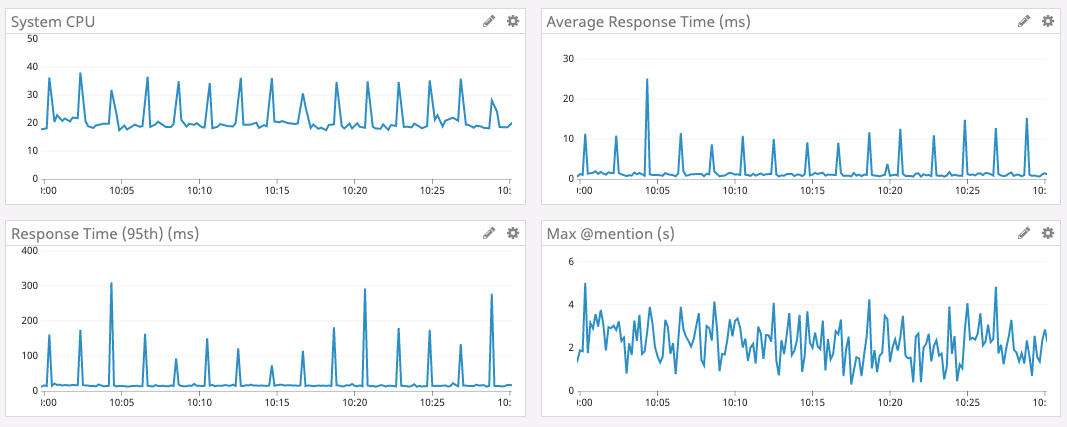
\includegraphics[width=0.8\textwidth]{images/golang-gc.png}
\end{center}

Quick recap: the Go garbage collector does its work and it adds a big latency spike. Rust would not have those spikes, because of ownership: when memory is no longer needed, it is trashed immediately and there's no waiting for the garbage collector to come by and decide if it can be cleaned up. To be fair, C++ also wouldn't have such spikes (because RAII). The article also adds that even with basic optimization, the Rust version performed better than the Go version. Not only in terms of there being no spikes, but in many dimensions: latency, CPU, and memory usage.

See the following graphs that compare Rust (blue) to Go (purple): 
\begin{center}
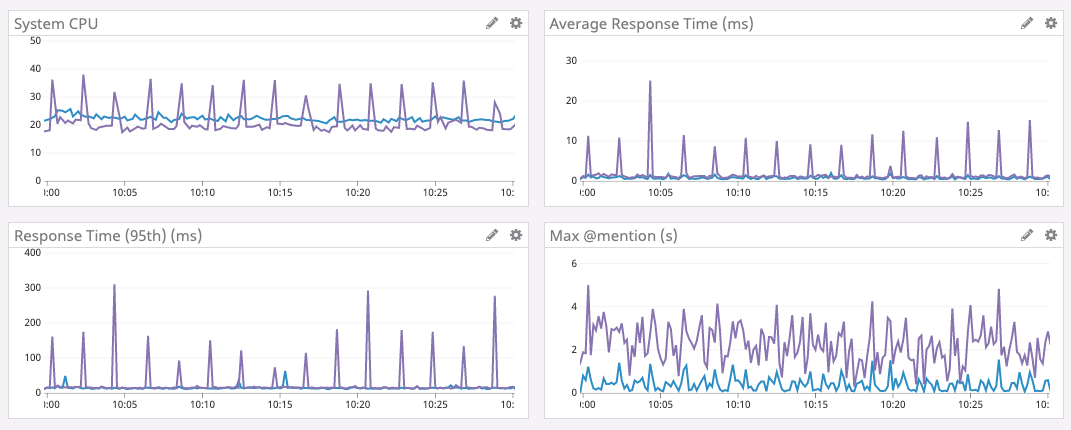
\includegraphics[width=0.8\textwidth]{images/rust-vs-go.png}
\end{center}

I do recommend reading the article because it goes into some more details and may answer some questions that you have. 

\paragraph{The Rules.}
That long introduction to the concept of ownership didn't explain very much about how it actually works; it just went into the \textit{why} and how it relates to the objectives of this course. But the rules are pretty simple---deceptively so---and they are as follows:

\begin{enumerate}
	\item Every value has a variable that is its owner.
	\item There can be only one owner at a time.
	\item When the owner goes out of scope, the value is dropped.
\end{enumerate}

These rules draw a distinction between the value itself and the variable that owns it. So in a statement of \texttt{let x = 42;} there is memory associated with the value "42". That memory is the "value" in rule 1, and its owner is the variable \texttt{x}.

When \texttt{x} goes out of scope, then the memory will be deallocated (``dropped''). (This is very much like the RAII (Resource Acquisition Is Initialization) pattern in languages like \CPP). Variable scope rules look like scope rules in other C-like languages. We won't belabour the point by talking too much about scope rules. But keep in mind that they are rigidly enforced by the compiler. See a brief example:
\begin{lstlisting}[language=Rust]
  fn foo() {
    println!("start");
    { // s does not exist
      let s = "Hello World!";
      println!("{}", s);
    } // s goes out of scope and is dropped
  }
\end{lstlisting}

The same principle applies in terms of heap allocated memory (yes, in Rust you cannot just pretend there's no difference between stack and heap, but ownership helps reduce the amount of mental energy you need to devote to this). Let's learn how to work with those! The example we will use is \texttt{String} which is the heap allocated type and not a string literal. We create it using the 
\begin{lstlisting}[language=Rust]
  fn main() {
    let s1 = String::from("hello");
    println!("s1 = {}", s1);
  }
\end{lstlisting}

A string has a stack part (left) and a heap part (right) that look like~\cite{rustdocs}:
\begin{center}
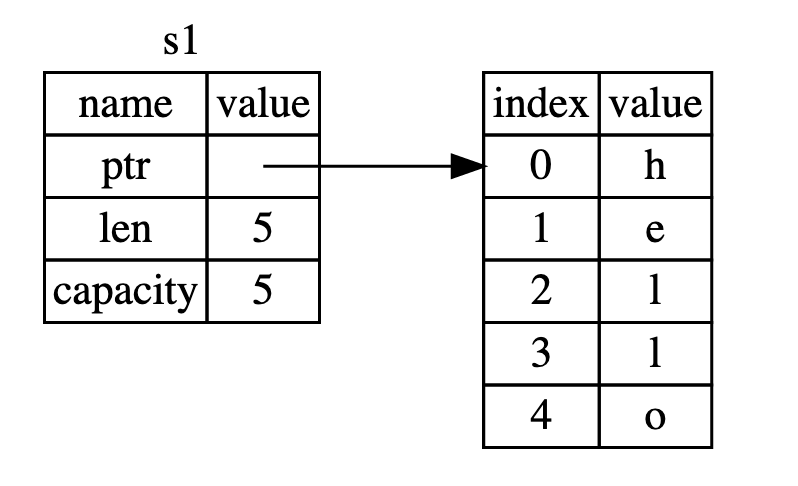
\includegraphics[width=0.33\textwidth]{images/string.png} 
\end{center}

This makes it a bit clearer about what is meant when the rules say that when the owner (the stack part) goes out of scope, the value (the heap part) is deallocated.

That covers rules one and three\ldots But that second rule is interesting, because of the ``at a time'' at the end: it means that there exists the concept of transfer of ownership.

In fact, everything we've said so far could also be true for much \CPP~code using RAII: there is an owner for each value, there is only one owner, and things are freed when they go out of scope. However, ``there is only one owner'' isn't actually enforced by the \CPP~compiler, so you can write code that breaks it, and then that code is prone to segfaults. 

\paragraph{What's yours is mine.}
Move semantics have to do with transferring ownership from one variable to another. But ownership is overkill for simple types\footnote{Specifically, types with the \texttt{Copy} trait have copy semantics by default; this trait is mutually exclusive with the \texttt{Drop} trait. \texttt{Copy} types have known size at compile time and can be stack-allocated.} (see the docs for a list---stuff like integers and booleans and floating point types), and such types don't need to follow move semantics; they follow copy semantics. Copy semantics are great when copies are cheap and moving would be cumbersome. So the following code creates two integers and they both have the same value (5).

\begin{lstlisting}[language=Rust]
  fn main() {
   	let x = 5;
	let y = x;
  }
\end{lstlisting}

But simple types are the exception and not the rule. Let's look at what happens with types with a heap component:

\begin{lstlisting}[language=Rust]
  fn main() {
    let s1 = String::from("hello");
    let s2 = s1;
  }
\end{lstlisting}

Here, no copy is created. For performance reasons, Rust won't automatically create a copy if you don't ask explicitly. (You ask explicitly by calling \texttt{clone()}). Cloning an object can be very expensive since it involves an arbitrary amount of memory allocation and data copying. This point is a thing that students frequently get wrong in ECE~252 in that that when doing a pointer assignment like \texttt{ thing* p = (thing*) ptr;} that no new heap memory was allocated and we have \texttt{p} and \texttt{ptr} pointing to the same thing. But that's not what happens in Rust~\cite{rustdocs}:

\begin{center}
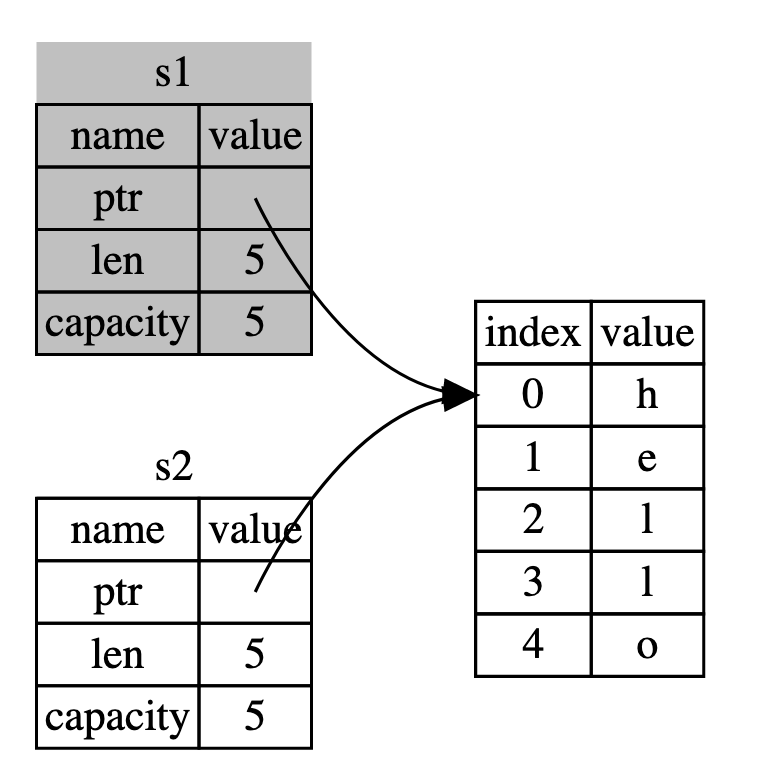
\includegraphics[width=0.3\textwidth]{images/string-rust.png}
\end{center}

If both \texttt{s1} and \texttt{s2} were pointing to the same heap memory, it would violate the second rule of ownership: there can be only one! So when the assignment statement happens of \texttt{let s2 = s1;} that transfers ownership of the heap memory to \texttt{s2} and then \texttt{s1} is no longer valid. There's no error yet, but an attempt to use \texttt{s1} will result in a compile-time error. Let's see what happens.

\begin{lstlisting}[language=Rust]
  fn main() {
    let x = 5;
    let y = x;
    dbg!(x, y); // Works as you would expect!

    let x = Vec<u32>::new(); // similar to the std::vector type in C++
    let y = x;
    dbg!(x, y); // x has been moved, this is a compiler error!
  }
\end{lstlisting}

The compiler is even kind enough to tell you what went wrong and why (and is super helpful in this regard compared to many other compilers)~\cite{rustdocs}:
\begin{verbatim}
plam@amqui ~/c/p/l/l/L02> cargo run
   Compiling move v0.1.0 (/home/plam/courses/p4p/lectures/live-coding/L02)
error[E0382]: use of moved value: `x`
 --> src/main.rs:8:10
  |
6 |     let x = Vec::<u32>::new(); // similar to the std::vector type in C++
  |         - move occurs because `x` has type `std::vec::Vec<u32>`, which does 
              not implement the `Copy` trait
7 |     let y = x;
  |             - value moved here
8 |     dbg!(x, y); // x has been moved, this is a compiler error!
  |          ^ value used here after move

error: aborting due to previous error

For more information about this error, try `rustc --explain E0382`.
error: could not compile `move`.

To learn more, run the command again with --verbose.
\end{verbatim}

Move semantics also make sense when returning a value from a function. In the example below, the heap memory that's allocated in the \texttt{make\_string} function still exists after the reference \texttt{s} has gone out of scope because ownership is transferred by the \texttt{return} statement to the variable \texttt{s1} in \texttt{main}.

\begin{lstlisting}[language=Rust]
  fn make_string() -> String {
    let s = String::from("hello");
    return s;
  }

  fn main() {
    let s1 = make_string();
    println!("{}", s1);
  }
\end{lstlisting}

This works in the other direction, too: passing a variable as an argument to a function results in either a move or a copy (depending on the type). You can have them back when you're done only if the function in question explicitly returns it! 

\begin{lstlisting}[language=Rust]
  fn main() {
    let s1 = String::from("world");
	use_string( s1 ); // Transfers ownership to the function being called
	// Can't use s1 anymore!
  }
  
fn use_string(s: String) {
    println!("{}", s); 
    // String is no longer in scope - dropped
}
\end{lstlisting}

This example is easy to fix because we can just add a return type to the function and then return the value so it goes back to the calling function. Great, but what if the function takes multiple arguments that we want back? We can \texttt{clone()} them all\ldots which kind of sucks. We can put them together in a package (structure/class/tuple) and return that. Or, we can let the function borrow it rather than take it\ldots But that's for next time!

\CPP~does have move semantics, but it uses copy semantics by default.

\paragraph{Do the Rules Work?}
With a stronger understanding of the rules and their practicalities, the obvious question is: do they work\textinterrobang~There's no point in having the rules if they don't accomplish the goal. We'll assume for the moment that there are no bugs in the compiler that violate the expected behaviour. And then let's consider this from the perspective of some things that can go wrong in a C program.

(Okay, alright, before we get there---we'll eventually learn to break rules and to use reference counted objects where if we get it wrong we can leak. We briefly discuss \texttt{Rc} and \texttt{Arc} in Lecture 4.)

\begin{itemize}
	\item Memory leak (fail to deallocate memory)---does not happen in Rust because the memory will always be deallocated when its owner goes out of scope.
	\item Double-free---does not happen in Rust because deallocation happens when the owner goes out of scope and there can only be one owner.
	\item Use-after-free---does not happen in Rust because a reference that is no longer valid results in a compile time error.
	\item Accessing uninitialized memory---caught by the compiler.
	\item Stack values going out of scope when a function ends---the compiler will require this be moved or copied before it goes out of scope if it is still needed.
\end{itemize}

\subsection*{A free lunch?}
To provide a somewhat balanced view, Rust of course doesn't solve every problem
in the world. It does solve memory management well, and I wouldn't even say that
it requires more of the programmer: it requires more of the programmer at compile-time,
not at debug-time.

Let's revisit garbage collection. If you want
to implement graphs and doubly-linked lists\footnote{\url{https://rust-unofficial.github.io/too-many-lists/}}, GC is really handy. (Many
Rust people will argue that you shouldn't use linked lists if you want
performance anyway. If you think back to your architecture course, you
can deduce why.) Or you can use pointers and unsafe Rust and hope to
get it right.


Here are some downsides to consider:
\begin{itemize}
\item Static typing: To expand on the point above: there is a New Zealand saying ``she'll be right''. It's a bit hard to explain, but Wikipedia suggests: ``a situation or object which is not perfect but is good enough to fulfil its purpose''. Static typing, and Rust, discourage this point of view. The code really does have to satisfy type safety and memory safety properties before it will run.
\item Ecosystem: Rust does come with a package registry (crates), which is better than \CPP, but some libraries are not going to exist in Rust. We'll talk more about calling foreign functions in Lecture 5.
\item Compiler: Rust's compiler can be slow on large codebases.
\end{itemize}










\chapter*{3 --- Rust: Borrowing, Slices, Threads, Traits}

\addcontentsline{toc}{chapter}{3 --- Rust: Borrowing, Slices, Threads, Traits}

\section*{Borrowing and References}
We've already seen that ownership is a concept in Rust that can come with a couple of unintended consequences, e.g. from accidentally giving an argument to a function that we still need later. Rust supports ``borrowing''---you need to use the data for something but you also promise you'll give it back (and the compiler forces you to live up to your promises). Borrowing allows data to be shared, but the sharing has to be done in a controlled and safe way to prevent leaks and race conditions.

Rust's compiler analyzes all the borrowing that takes place in the program using the \textit{borrow checker}. If the borrow checker is not certain that your code is perfectly safe, it will say no (and produce a compile time error). This can be a little bit frustrating, because the analysis is not perfect and errs on the side of caution. Eventually we will introduce some ways that you can tell the borrow checker that you guarantee the code is safe, but you have to be sure, otherwise all the usual bad things can happen!

The feature that we need for the concept of borrowing is the \textit{reference}. To indicate that you want to use a reference, use the \texttt{\&} operator. The reference operator appears both on the function definition and the invocation, to make sure there's no possibility of confusion as to whether a reference is being expected/provided or ownership is to be transferred.  Consider this example from the official docs~\cite{rustdocs}:

\begin{lstlisting}[language=Rust]
fn main() {
    let s1 = String::from("hello");
    let len = calculate_length(&s1);
    println!("The length of '{}' is {}.", s1, len);
}

fn calculate_length(s: &String) -> usize {
    s.len()
}
\end{lstlisting}

When we invoke the \texttt{calculate\_length} function, ownership of the string is not transferred, but instead a reference to it is provided. The reference goes out of scope at the end of the function where it was used, removing it from consideration. A reference is not the same as ownership and the reference cannot exist without the original owner continuing to exist. That is represented in the official docs by this diagram:

\begin{center}
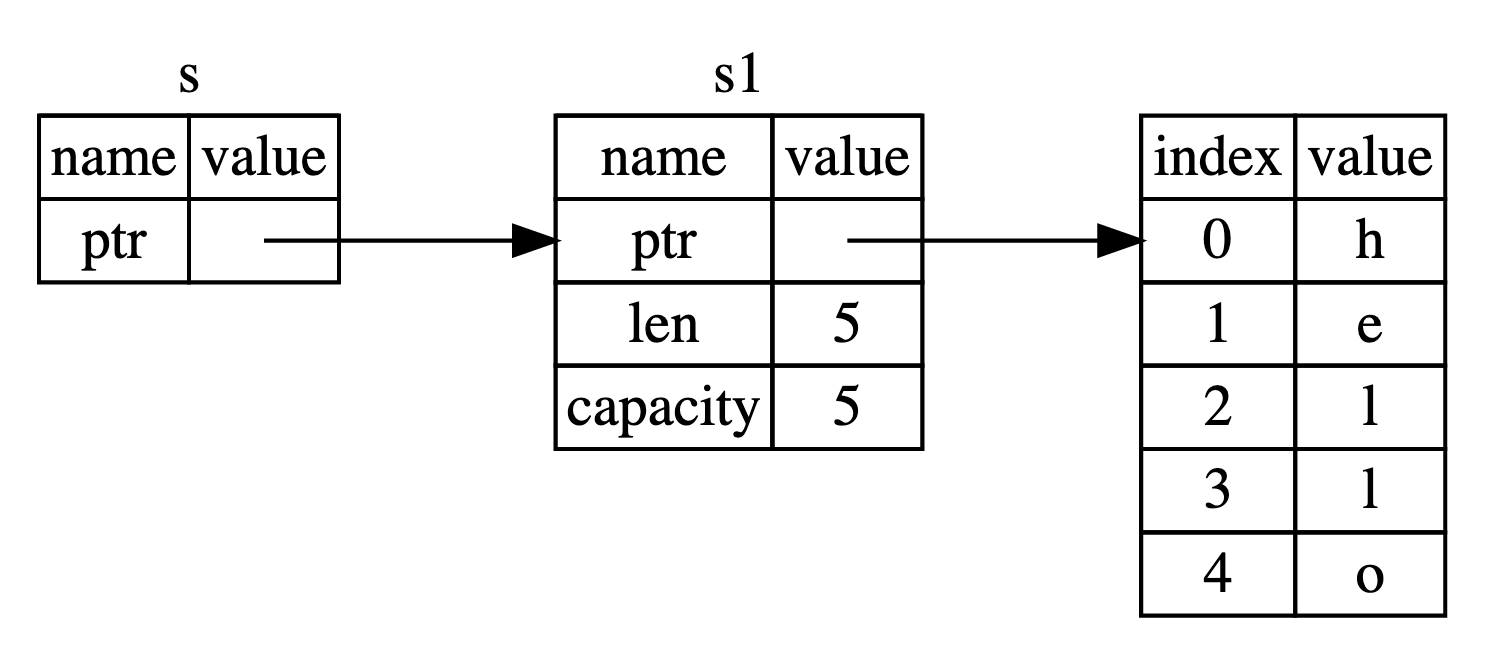
\includegraphics[width=0.5\textwidth]{images/string-with-ref.png}
\end{center}

And if you borrow something, it's not yours to do with as you wish---you cannot assign ownership of it (move it), which makes sense because you can't give someone ownership of something you do not own.

By default, references are immutable: if you borrow something, you cannot change it, even if the underlying data is mutable. Attempting to do so will result in---you guessed it---a compile time error, where the compiler tells you that you are trying to change something that's immutable. 

Of course, in real life, you would be much more agreeable to letting people borrow your things if there were strong guarantees that it would (1) always be returned and (2) would be returned in the same condition. That would be nice! But until such time as that magical technology is invented, no, you can't borrow my car. Sorry.

Mutable references do exist, but they have to be declared explicitly as such by tagging them as \texttt{\&mut}:

\begin{lstlisting}[language=Rust]
fn main() {
    let s1 = String::from("hello");
    let len = calculate_length(&mut s1);
    println!("The length of '{}' is {}.", s1, len);
}

fn calculate_length(s: &mut String) -> usize {
    s.len()
}
\end{lstlisting}

Mutable references come with  some big restrictions: (1) while a mutable reference exists, the owner can't change the data, and (2) there can be only one mutable reference at a time, and while there is, there can be no immutable references. This is, once again, to prevent the possibility of a race condition. These two restrictions ensure that there aren't concurrent accesses to the data when writes are possible. There's also a potential performance increase where values can be cached (including in CPU registers; we'll come to that later) without worry that they will get out of date.

As long as there are no mutable references, there can be arbitrarily many immutable references at the same time, because reads don't interfere with reads and a race condition does not occur if there are only reads. 

References cannot outlive their underlying objects. Below is an example from the official docs that will be rejected by the borrow checker, because the reference returned by \texttt{dangle} refers to memory whose owner \texttt{s} goes out of scope at the end of the function:

\begin{lstlisting}[language=Rust]
fn main() {
    let reference_to_nothing = dangle();
}

fn dangle() -> &String {
    let s = String::from("hello");
    &s
}
\end{lstlisting} 

In C this would be a ``dangling pointer'' (a pointer that's pointing to a location that is no longer valid). I see this kind of error a lot in C programs where someone has stack allocated a structure and then wants to pass it to another thread and does so with the address-of operator. It compiles and might even work sometimes at runtime, but is still wrong and can eventually be exposed as a bug that bites you.

If we actually try to compile the previous code example, the compiler says something about giving the value a lifetime. We'll come back to the idea of lifetimes soon.

\paragraph{Non-Lexical Lifetimes.} A more recent improvement to Rust's borrow checking is called non-lexical lifetimes. Consider the small block of code below:
\begin{lstlisting}[language=Rust]
fn main() {
    let mut x = 5;

    let y = &x;
    println!("{}", y);

    let z = &mut x;
}
\end{lstlisting}

Under the old rules, the compiler would not allow creation of the mutable reference \texttt{z} because \texttt{y} has not gone out of scope. It would consider \texttt{y} to be valid until the end of the function. The improvement of NLL is that the compiler can see that \texttt{y} is no longer used after the \texttt{println!} macro and hence the \texttt{z} reference is okay to create. \texttt{y} can be dropped as soon as it's no longer needed; the \texttt{z} reference will not exist at the same time; and all is fine.

\subsection*{Slices}
The \textit{slice} concept exists in a few other programming languages, and if you have experience with them this will certainly help. A slice is a reference (yes, a reference in the sense of the previous section) to a contiguous subset of the elements of a collection. This is what you do if you need a part of an array (the typical example for that being a substring of an existing string). If our code looks like this:

\begin{lstlisting}[language=Rust]
fn main() {
    let s = String::from("hello world");
    let hello = &s[0..5];
    let world = &s[6..11];
}
\end{lstlisting}

The representation of the slice looks like~\cite{rustdocs}:
\begin{center}
	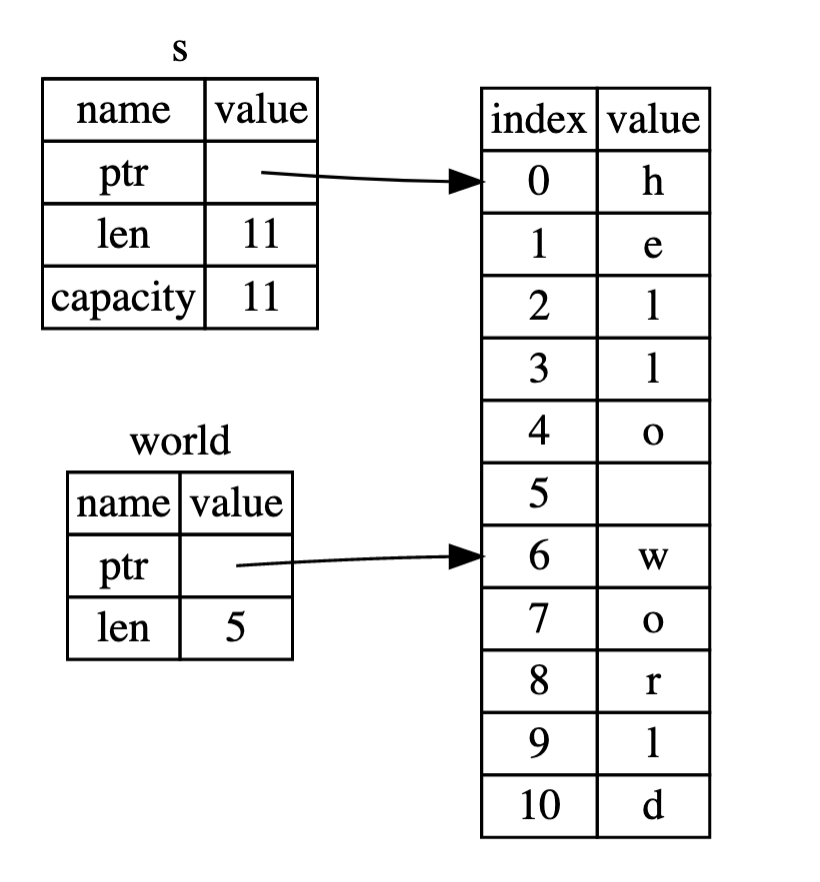
\includegraphics[width=0.3\textwidth]{images/string-slice.png}
\end{center}

Slices can also apply to vectors and other collections, not just strings. As with the other kinds of references we've learned about, the existence of a slice prevents modification of the underlying data. Just as with references, slices prevent race conditions on collections but also avoid (as much as possible) the need to copy data (slow).

\subsection*{Unwrap the Panic}
A quick digression: a lot of functions we use return \texttt{Result} types. These return either \texttt{Ok} with the type we expected, or \texttt{Err} with an error description. To get the type you want, you need to unpack the result.

If we try to open a file but the file doesn't exist, that's an error but one that's foreseeable and we can handle it. There's three ways to handle it: a \texttt{match} expression (this is like the \texttt{switch} statement), \texttt{unwrap()}, and \texttt{expect()}. 

You may be tempted to just always use \texttt{unwrap()} because it gives you the result and calls the \texttt{panic!} macro if there's an error. This, however, just shows you the lower level error that is the problem and you are denying yourself the opportunity to add information that will help you debug. For that reason, it's better to use \texttt{expect()}, which lets you add your own error message that will make it easier to find out where exactly things went wrong.

It's recommended to use \texttt{Result} types for functions you write too. Make your future self happy by giving yourself the information you need to debug what's gone wrong!

This does come at a small performance hit. CS~343 included a performance comparison of exceptions versus error codes (\`a la \texttt{Result}). Exceptions that don't happen (the happy path) are, indeed, faster than explicitly handling error codes / \texttt{Result} types. As an engineering trade-off, both exceptions and \texttt{Result} types force the programmer to explicitly deal with errors (at the very least, explicitly ignoring them rather than silently ignoring them). Rust doesn't have exceptions, so you always have to pay the performance hit. (Simulating exceptions with \texttt{panic!} is not a best practice.)

\section*{Fearless Concurrency}
More than just trying to prevent memory problems by making them compiler errors, Rust is also intended to make concurrency errors compile-time problems too! That's actually difficult, of course, but the good news is that the key ideas of ownership and borrowing and such will help you avoid concurrency problems.

The drawback to concurrency is that it brings new problems with it: race conditions, deadlock, that sort of thing. Making your program faster is great, but not if it's at the cost of the answers being incorrect (or your program failing to produce an answer some of the time).

If the compiler can help with making sure your concurrent program is correct, it doesn't make your program faster directly, but it helps indirectly. If you can be (more) sure of the correctness of your code, you don't have to spend as much time testing it before you can deploy it and move on to the next thing. Also, if the bug is prevented from being introduced in the first place, you don't have to spend time debugging it and fixing it, which lets you spend more time on speeding up other things. And honestly, if you are looking at a piece of code that is super business critical, anything that adds to your confidence that no issue has been introduced makes it that much easier to make that change you want to make.

\paragraph{Threads.} Rust uses threads for concurrency, with a model that resembles the create/join semantics of the POSIX pthread. If you are unfamiliar with pthreads, the course repository has a PDF refresher of the topic (\texttt{pthreads.pdf}). We will talk about the Rust way, but the background material will provide context.

So you want to create a thread! The mechanism for doing so is referred to as spawning a thread. Here's a quick example from the official docs~\cite{rustdocs}:

\begin{lstlisting}[language=Rust]
use std::thread;
use std::time::Duration;

fn main() {
    let handle = thread::spawn(|| {
        for i in 1..10 {
            println!("hi number {} from the spawned thread!", i);
            thread::sleep(Duration::from_millis(1));
        }
    });

    for i in 1..5 {
        println!("hi number {} from the main thread!", i);
        thread::sleep(Duration::from_millis(1));
    }

    handle.join().unwrap();
}
\end{lstlisting}

A few things make this significantly different from the pthread model that we are used to. First of all, the thread being created takes as its argument a \textit{closure}---an anonymous function that can capture some bits of its environment. The spawn call creates a \texttt{JoinHandle} type and that's what we use to call \texttt{join}, which is to say, wait for that thread to be finished. As we expect from pthreads, if calling join on a thread that is not finished, the caller waits until the thread is finished.

This is a simple example that works, but fails to capture the complexity of actually working with threads, because there's no data moved between threads. Most interesting uses of threads need some data communication. There are three ways that we can get data from one thread to another: capturing, message passing, and shared state.

\paragraph{Capturing.} 
The notion of ``capturing'' calls back to the earlier mention that a closure captures some of its environment. That is, the body of the function can reference variables that were declared outside of that function and in the context where \texttt{thread::spawn} was called. The compiler will analyze the request and try to figure out what needs to happen to make it work, such as borrowing the value, as in this example (also from the docs):

\begin{lstlisting}[language=Rust]
use std::thread;

fn main() {
    let v = vec![1, 2, 3];

    let handle = thread::spawn(|| {
        println!("Here's a vector: {:?}", v);
    });

    handle.join().unwrap();
}
\end{lstlisting}

The only problem is: this example does not work. The compiler is not sure how long the thread is going to live and therefore there's a risk that a reference to \texttt{v} held by the thread outlives the actual vector \texttt{v} in the main function. How do we fix that?

Well, I had the idea that if I put something after the \texttt{join()} call that uses \texttt{v}, then the compiler should know that \texttt{v} has to remain in existence until after the thread in question. Yet, it still reports the error E0373 that says the thread might outlive the borrowed value. This actually got me thinking about why this didn't work and I decided to ask some of the compiler devs. It has to do with the fact that a thread isn't really a first-class construct in Rust, and the ``lifetime'' of arguments that you pass has to be sufficiently long. We'll learn about lifetimes soon.

Anyway, the error message suggests what you actually want in this scenario: to move the variables into the thread. To do so, specify \texttt{move} before the closure: \texttt{let handle = thread::spawn(move || \{}\ldots~ This addition results in the transfer of ownership to the thread being created. You can also copy if you need. 

One thing you don't want to do is try to make the lifetime of your vector or other construct \texttt{static}, even though the compiler might suggest this. We can revisit that when we talk about lifetimes as well.

\paragraph{Message Passing.} Sometimes threads want to communicate in a way that isn't one-way communication at the time that the thread is being created. For that, a possibility is message-passing. This mechanism of communication may seem familiar from previous experience with various UNIX mechanisms like pipes and message queues. This strategy is very structured and generally safer than shared memory, i.e. it is harder to race or to access inappropriate locations.

The ownership mechanic of message passing is like that of postal mail. When you write a physical letter and mail it to someone, you relinquish your ownership of the letter when it goes in the mailbox, and when it is delivered to the recipient, the recipient takes ownership of that letter and can then do with it as they wish.

So you want to have two threads communicate. The Rust metaphor for this is called a \textit{channel}. It has a transmit end (where messages are submitted) and a receive end (where messages arrive). The standard model is multiple-producer, single-consumer: that is, lots of threads can send data via the sending end, but in the end it all gets delivered to one place. Think of that like postal mail as well: I can drop a letter to you in any postbox or post office, but they will all be delivered to your mailbox where you collect them in the end.

Okay, enough talk, let's make one~\cite{rustdocs}:
\begin{lstlisting}[language=Rust]
use std::sync::mpsc;
use std::thread;

fn main() {
    let (tx, rx) = mpsc::channel();

    thread::spawn(move || {
        let val = String::from("hi");
        tx.send(val).unwrap();
    });

    let received = rx.recv().unwrap();
    println!("Got: {}", received);
}
\end{lstlisting}

The channel constructor returns a tuple with the transmitting end \texttt{tx} and receiving end \texttt{rx}. We'll then send the transmitting end into the thread and have it send a message to the main thread. The main thread will wait until the message is there and then get it. This does mean that \texttt{recv()} is blocking and there is a corresponding \texttt{try\_recv()} which is nonblocking. You may have already covered nonblocking I/O in a previous course; if not, we will return to that subject soon.

If you want to have multiple transmitting ends, you need only use \texttt{clone} on the transmitter and hand those out as needed. 

As a small technical note, the type you want to send via a channel has to implement the \texttt{Send} trait (think of traits being like interfaces). Almost all basic types in Rust have this trait, and any programmer-defined type that is composed entirely of types that have it will also have that trait.  


\subsection*{Traits}
Okay, we have to take a detour here onto the subject of Traits. As the previous paragraph said, traits are a lot like interfaces. You specify a trait as a set of function signatures that you expect that the type in question to implement. A very simple trait and its usage are shown below:

\begin{lstlisting}[language=Rust]
pub trait FinalGrade {
	fun final_grade(&self) -> f32;
}

impl FinalGrade for Enrolled_Student {
    fn final_grade(&self) -> f32 {
        // Calculation of average according to syllabus rules goes here
    }	
}  
\end{lstlisting}

A couple of other notes about traits are worth mentioning. One, you can only define traits on your own types, not on external (from other packages/crates) types, so that you don't break someone else's code. Two, you can add a default implementation to the trait if you want (something Java lacked for a long time). Third, as in other languages with interfaces, a trait can be used as a return type or method parameter, so it is a kind of generic. Finally, you can use \texttt{+} to combine multiple traits (which is nice when you need a parameter to be two things)

With the preamble out of the way, there are three traits that are really important to us right now. They are \texttt{Iterator}, \texttt{Send}, and \texttt{Sync}. 

Iterator is the easiest one to explain. You put it on a collection and it allows you to iterate over the collection. Moreover, this is often more efficient than a typical for loop construction, because it lets the compiler skip over bounds checking and other such issues. Nice.

Send was already introduced. It's necessary to transfer ownership between threads. There are some Rust built-in or standard-library types that very specifically choose not to implement this interface to give you a hint that they are not intended for this purpose. If the compiler tells you no, it's a hint that you want to use a different type. As previously mentioned, if your programmer-defined type is made entirely of types that have the Send trait, then it too has the trait. If you really must use something that is inherently not safe to send, though, you can implement this trait on your type manually and guarantee the thread-safe transfer of ownership yourself, but it's not a good idea if you can avoid it.

Sync is the last one, and it means that a particular type is thread-safe. That means it can be referenced from multiple threads without issue. The primitive types have this trait, as do any programmer-defined types that are composed entirely of Sync types. It's important to just mention here that this does not mean all operations on a Sync type are safe and that no race conditions are possible; it just means that \textit{references} to the type can be in different threads concurrently, and we can't have multiple mutable references. No, if we want more than one thread to be able to modify the value, we need mutual exclusion...

\subsection*{Back to the Mutex...}
If you don't want to use message passing for some reason (and performance is a reason, if it's borne out by your testing/data) then there is fortunately the ability to use a mutex for mutual exclusion. We know how these work, so let's skip the part where I make some analogy about them. 

What's different about the mutex in Rust is that the Mutex wraps a particular type. So it is defined as \texttt{Mutex<T>} and if you want an integer counter, you create it as \texttt{Mutex::new(0);}. This way, the mutex goes with the value it is protecting, making it much more obvious what mutex goes with what data, and making it so you have to have the mutex to access the data. And sample from the docs~\cite{rustdocs}:

\begin{lstlisting}[language=Rust]
use std::sync::Mutex;

fn main() {
    let m = Mutex::new(5);

    {
        let mut num = m.lock().unwrap();
        *num = 6;
    }

    println!("m = {:?}", m);
}
\end{lstlisting}

In addition to forcing you to acquire the mutex before you can make any use of the internal value, the lock is automatically released when the \texttt{num} variable goes out of scope; the type of \texttt{num} is a \texttt{MutexGuard} which is our ``possession'' of the lock; when that possession ends, the mutex is automatically unlocked. This means you want, generally, to use the manual-scoping \texttt{ \{ } and \texttt{ \} } braces to ensure that the lock is released when you're done with it and not just at the end of the function or loop.

The use of the mutex in the above program is obviously unnecessary, since there's only the one thread. If we want to use it in multiple threads, we need multiple threads to access it. But we can't, unfortunately, just say that references will do! The mutex type has to outlive the other threads and such and the compiler will suggest moving it... But we can't move it into more than one thread, because that violates our rule about having only one owner. What now?

It looks like we have to break a rule: we need the ability to share ownership of some memory. We don't know how to do that, but when we start with breaking rules, we might find that we like it and might break more than one\ldots










\chapter*{4 --- Rust: Breaking the Rules for Fun and Performance}

\addcontentsline{toc}{chapter}{4 --- Rust: Breaking the Rules for Fun and Performance}

\section*{Mutual Exclusion and Multiple Ownership}

\paragraph{Mutex and Reference Counting}

Where we left off previously, we've identified that a mutex is not super amenable to our model of single ownership because we need multiple threads to have access to this mutex. There is a way to do it, but we have to break the single ownership rule, and that requires a little more background on smart pointers and reference counting.

We know what pointers are from C and \CPP, and if you have sufficient experience with \CPP{ }you will know that smart pointers exist in that language too! We'll talk about two kinds of smart pointer right now, the Box and the Reference-Counting type.

The \texttt{Box<T>} is an easy way to put some data on the heap rather than the stack. This is good for a situation where you, for example, take input from a user and you don't know in advance how big it's going to be, or when you have some data that you want to transfer ownership of rather than copy (for performance reasons, obviously). You create a Box with \texttt{Box::new(...)} as expected, and it's heap allocated with all the usual things that come with it in Rust, like ownership and that it gets dropped if the owner goes out of scope.

The reference counted smart pointer, however, is the thing that allows for shared ownership. There are some reasons why we might want this, even in a single-threaded program, such as a graph data structure. But the main idea is that you can share ownership as much as you like, and the value only goes away when the last reference to it is dropped (reference count goes to zero). 

To make a reference-counted object, use type \texttt{Rc<T>}. Instantiate that type to get an object; if you want to make another reference to the same object, use \texttt{clone()}, which increases the reference count. When references are dropped, the count decreases.

It is important to note that reference types can leak memory! If you've chosen this route for managing data in your program, there is a possibility of forming a cycle in the reference types. If such a cycle is formed, the memory will never be dropped. This is undesirable, of course.

What you can't do, unlike \CPP's analogous \texttt{shared\_ptr}, is keep a reference to the value after the \texttt{Rc} or \texttt{Arc} goes out of scope. That's because the value is still owned by the pointer and is definitely freed when the pointer goes away.

Right, so we have everything we need now to pass the mutex around, right? Well, almost. \texttt{Rc<T>} won't work when we try to pass it between threads, because the compiler says it cannot be sent between threads safely. This is because the management of its internal counter is not done in a thread-safe way. If we want that, we need the \textit{atomic} reference counted type, which is \texttt{Arc<T>}. It is perhaps slightly slower than the regular reference counted type, so you won't want to choose it in every scenario, but it's exactly what we need here.

Here's an example of using an atomic reference counted type for setting up a handler for the Ctrl-C (SIGINT); this is modified from a program I wrote that listens for connections and spawns threads if a client connects: 

\begin{lstlisting}[language=Rust]
use std::sync::Arc;
use std::sync::atomic::{AtomicBool, Ordering};

fn main() {
   let quit = Arc::new(Mutex::new(false));
    let handler_quit = Arc::clone(&quit);
    ctrlc::set_handler(move || {
        let mut b = handler_quit.lock().unwrap();
        *b = true;
    }).expect("Error setting Ctrl-C handler");
 
    while !(*quit.lock().unwrap()) {
    	// Do things
    }
}
\end{lstlisting}

In this example, I use a mutex to protect a boolean that's used concurrently (even if it's not in two threads): once in main and once in the handler. 

We should also still remember that there exists the possibility of a deadlock in Rust, even if the mutex is automatically unlocked for us. Nothing prevents thread 1 from acquiring mutex A then B and thread 2 from concurrently acquiring B then A. This language cannot solve all concurrency problems, unfortunately.

\section*{Lifetimes}
We've covered the idea that in Rust, the compiler can make a determination about how long a particular piece of data will live. How long it lives is sometimes referred to as the reference's lifetime. The good news is that the compiler is usually able to make a determination about how long things should live. This system is not perfect, and sometimes we have to help it a bit.

Here's a simple program in the official docs that won't compile because the type system can't figure out what's correct~\cite{rustdocs}:

\begin{lstlisting}[language=Rust]
fn main() {
    let string1 = String::from("abcd");
    let string2 = "xyz";

    let result = longest(string1.as_str(), string2);
    println!("The longest string is {}", result);
}

fn longest(x: &str, y: &str) -> &str {
    if x.len() > y.len() {
        x
    } else {
        y
    }
}
\end{lstlisting}

The compiler says it can't figure out whether the return value is the borrowing of \texttt{x} or \texttt{y} and therefore it's not sure how long those strings live. It might look like it's obvious at this point, because the two strings are known at compile time. The compiler, however, makes decisions based on local information only (that is, what it finds in the current function it is evaluating). For that reason, it treats \texttt{longest} as if it could take any two string references. Alright, that's fine for now, because it was an example to show what happens when we can't know the answer at compile time anyway.

To get this to compile, we have to specify lifetimes using annotations. Annotations don't change how long references live, really. They just describe the relationships between the lifetimes of references. This is used on functions to specify what they can accept and what they can return.

If you'd like an analogy, think of it as saying something like ``I will only buy eggs that have an expiration date that is at least two weeks in the future.''. This rule does not change the eggs that are in the store. It does not mean that eggs that have an expiration date of next week are poison and nobody should eat them. I'll happily buy eggs that expire in a month. So we are just being clear about what we want here.

Lifetime annotations are written with an apostrophe \texttt{'} followed by a name, and names are usually short like \texttt{'a} or \texttt{'b}. Let's correct the \texttt{longest} function:

\begin{lstlisting}[language=Rust]
fn longest<'a>(x: &'a str, y: &'a str) -> &'a str {
    if x.len() > y.len() {
        x
    } else {
        y
    }
}
\end{lstlisting}

This does what we need! The first appearance, after the name of the function, of our lifetime annotation says that all parameters and return value must have the same lifetime. Then we say we will accept strings that live at least as long as our designated \texttt{'a} lifetime. That is, it's got to live at least as long as the smallest of \texttt{x} and \texttt{y}. The actual lifetime isn't as important, all that matters is that it follows the rule of being at least that long.

In early versions of Rust, lifetime annotations had to be specified everywhere. That was somewhat annoying, but fortunately the compiler can identify a lot of common scenarios, so the borrow checker can read them in where they're needed most of the time.


But we're not breaking rules here, we're applying more rules. What gives? The rule-breaking thing is the ability to grant a particular piece of memory immortality. If you specify as a lifetime the special one \texttt{'static}, you grant the ability for this memory to live the entire duration of the program. Just because it can doesn't mean it necessarily will live forever---only that it could. 

This can be used correctly to tell the compiler that a particular reference will always be valid, such as string literals that are always going to hang around. It's also used in the interface for spawning a thread, incidentally, which happens because you can pass \textit{anything} to a thread, and the compiler wants to be sure that whatever you are providing is definitely going to live long enough for the thread which can live an arbitrarily-long life (threads are estimated to be immortal). 

For the record, the kind of immortality we are talking about here is the Tolkien-Elf kind, where they won't die of old age, but can die in violence or grief. Threads can exit and be cancelled and such in Rust, and static variables can get dropped if the compiler is sure it's safe to do. But they \textit{could} hang around indefinitely.

You can use the static lifetime to bandaid a couple of compiler errors, and the compiler might even suggest it. You shouldn't, though, you should really apply the correct lifetime annotations or fix the would-be dangling reference. The compiler can lead you down the wrong path if it says that it wants a vector being passed to a thread to be annotated as static. What you might think is that it means you should annotate the function parameter with this lifetime, but that just moves the pain to where the function is called. So you modify those and it goes up the chain until you're at creation of the vector and you're left wondering how to make it have a static lifetime. Really, what the compiler means is that a reference isn't appropriate and you need to either move the data, copy the data, or use some other construct like the \texttt{Arc} (atomic reference counter) that is appropriate to the situation. 

Memory that's kept around forever that is no longer useful is fundamentally very much like a memory leak, even if it is still possible to deallocate it in a hypothetical sense.

\section*{Holodeck Safeties are Offline}
There's one last thing that we need, and it is dark and terrible magic. It is \textit{unsafe}. Unsafe exists because it has to. The compiler would rather err on the side of caution and say no to a program that is correct, than say yes to one that isn't. You might also need to interact with some other library or do some very low-level stuff. For this reason, we can override this and tell the compiler that you promise you know this is okay. You do so at your own risk, though, because you can get it wrong and if you do you get all the same problems Rust tries to avoid, like segmentation faults and memory leaks.

To do anything that qualifies as unsafe, you can go one of two ways. Either you declare a block as \texttt{unsafe}, or you specify that a given function is \texttt{unsafe} by putting that in the function signature. Inside an unsafe block or function, you can do the following things that you are not normally allowed to do~\cite{rustdocs}:

\begin{enumerate}
	\item Call an unsafe function/method
	\item Access or modify a mutable static variable
	\item Implement an unsafe trait
	\item Access the fields of a \texttt{union}
	\item Dereference a raw pointer
\end{enumerate}

That list is probably less extensive than you were expecting. Declaring a block as unsafe does not grant you unlimited power, sadly. The borrow checker still does its thing and there are still rules. 

The design intentions for unsafe blocks are that they are supposed to be small (this reduces the chance of an error and makes it easier to find) and ideally are abstracted away a bit behind some interface\ldots

\paragraph{Danger Zone.} The easiest example to show is what happens when you want to call a function that is unsafe. Suppose we have a function \texttt{do\_unsafe\_thing()}; its function signature will be something like \texttt{unsafe fn do\_unsafe\_thing()} and to call it, we must wrap it in an unsafe block:

\begin{lstlisting}[language=Rust]
unsafe {
  do_unsafe_thing();
}
\end{lstlisting}

Unsafe things are clearly designated in both ways: when you write a function that is unsafe, you declare to the world that this function is unsafe. Then, anyone who wants to use it also has to acknowledge that they know the function in question is unsafe. (Readbacks are a safety convention used in aviation, among other places.)

If you try to use an unsafe function without it being in an unsafe block, the compiler will, naturally, forbid such a thing. Just smashing the unsafe block around it is enough to make the compiler quiet, but not a thorough code reviewer. They would ask about whether you've read carefully the documentation of the function in question and whether you are sure you're calling it with the right arguments\ldots You did read the documentation, right? Right?

\paragraph{Mutable static variables.} Rust tries pretty hard to discourage you from using global variables, and they are right to do so. It's a quick shortcut and we do it a lot in course assignments, exercises, labs, and even exam questions. On an exam question, the thing I want to test is something like how you use the mutex and queue constructs to solve the problem, not how well you pass the mutex and queue pointers from the main thread to the newly created threads. In production code, though, global variables are really not recommended because of how harmful it is to good software engineering principles. 

But anyway, you can make global variables mutable in Rust, if you must, and do so you have to mark this as unsafe. But if you find yourself doing such a thing, please stop and think very carefully about why.

\paragraph{Implement an unsafe trait.} Appropriately, if the trait (interface) you want to implement has unsafe in the function signature, the compiler forces you to admit that your code is unsafe. If you do, it mostly means that you have to guarantee that what you're doing does in fact meet the requirements the interface specifies (like \texttt{Send}).

\paragraph{Unions.}
In C, there exists the concept of the \texttt{union}\footnote{\url{https://en.wikipedia.org/wiki/Union_type}}. You might not have heard of it because a lot of people don't like it (and I'm one of them). You might have to contend with it in a particular API.  It's like a \texttt{struct}, except where a \texttt{struct} is all of the contents (e.g., an integer and a floating point number and a pointer), a \texttt{union} is only one of those at a time (an integer or a floating point number or a pointer). Because there's no way to be totally sure that the \texttt{union} you're looking at is in fact the type you expect it to contain, you can only access the members in an unsafe block. 


\paragraph{Raw pointers.}
You can create raw pointers anywhere you like, but to dereference them, that has to be in an unsafe block. Creating the raw pointers can't cause a program crash; only using them does that. Of course, creating them incorrectly guarantees that when you try to use them they blow up in your face. I guess blame is a tricky subject.

Here's an example from the official docs~\cite{rustdocs}:
\begin{lstlisting}[language=Rust]
let mut num = 5;

let r1 = &num as *const i32;
let r2 = &mut num as *mut i32;

unsafe {
    println!("r1 is: {}", *r1);
    println!("r2 is: {}", *r2);
}
\end{lstlisting}

You can also use raw pointers when you need to write to a particular memory address, which sometimes happens for memory-mapped I/O. You just assign your value to an integer (i.e., \texttt{let add = 0xDEADBEEF}) and then cast it to a raw pointer (which is of type \texttt{*const}). When you want to write some data to that address, use the unsafe block and write it.

You might need this if you are calling into a C library or function. The Rust universe of packages (``crates'') is getting larger all the time, but sometimes you'll have to interact with a library in C\ldots or write a part of your application in Rust that is called from C. There is a crate for cURL, but it might be interesting to learn what one would have to do to use the C library for it\ldots

\paragraph{Rust vs \CPP.} Now that you know all about Rust, you can see a discussion of the \CPP~equivalents here: \url{https://reberhardt.com/cs110l/spring-2020/slides/lecture-18.pdf#page=27}. Basically everything in Rust also exists in \CPP, but \CPP~doesn't make you use these things in a safe way.









\chapter*{5 --- Asynchronous I/O}

\addcontentsline{toc}{chapter}{5 --- Asynchronous I/O}

\section*{Asynchronous/non-blocking I/O}

\begin{center}
  \fbox{
\includegraphics[width=.7\textwidth]{images/L05-tokio.png}}
\end{center}

To motivate the need for non-blocking I/O, consider some standard I/O code:

\begin{lstlisting}[language=Rust]
fn main() -> io::Result<()> {
  let mut file = File::open("hello.txt")?;
  let mut s = String::new();
  file.read_to_string(&mut s)?;
  Ok(()) 
}
\end{lstlisting}
(The ? operator ``for easier error handling'' is an alternative to
\texttt{try!} and \texttt{unwrap}.)

This isn't very performant. The problem is that the {\tt read} call will
{\em block}. So, your program doesn't get to use the zillions of CPU cycles that
are happening while the I/O operation is occurring.

\paragraph{As seen previously: threads.} Threads can be fine if
you have some other code running to do work---for instance, other threads
do a good job mitigating the I/O latency, perhaps doing I/O themselves.
But maybe you would rather not use threads. Why not?
\begin{itemize}[noitemsep,topsep=-1em]
\item potential race conditions;
\item overhead due to per-thread stacks; or
\item limitations due to maximum numbers of threads.
\end{itemize}

\subsection*{Doing non-blocking I/O}
We're going to focus on low-level I/O from sockets in this part of the lecture,
using the \texttt{mio}\footnote{\url{https://tokio-rs.github.io/mio/doc/mio/}} library from \texttt{tokio}. Async file I/O is
also possible via \texttt{tokio::fs} and the ideas will carry over.
One might often want to wrap the low-level I/O using higher-level
abstractions, and the larger project \texttt{tokio.rs} is one way of
doing that.

Fundamentally,
there are two ways to find out whether I/O is ready to be queried:
polling (under UNIX, implemented via {\tt select}, {\tt poll}, and
{\tt epoll}) and interrupts (under UNIX, signals). \texttt{mio}
supports polling-based approaches and abstracts across Linux (via
epoll), Windows (via IOCP), and BSDs including MacOS (via kqueue).

The key idea is to give {\tt mio} a bunch of event sources and
wait for events to happen. In particular:
     \begin{itemize}[noitemsep,topsep=-1em]
       \item create a \texttt{Poll} instance;
       \item populate it with event sources e.g. \texttt{TCPListener}s; and,
       \item wait for events in an event loop ({\tt Poll::poll()}).
     \end{itemize}
Let's run through these steps in order, following \url{https://docs.rs/mio/0.7.0/mio/guide/index.html}:

\paragraph{Creating a {\tt Poll} instance.} Just use the API:
    \begin{lstlisting}[language=Rust]
let poll = Poll::new()?;
let events = Events::with_capacity(128);
    \end{lstlisting}
We're going to proactively create \texttt{events}; this data structure is used by
\texttt{Poll::poll} to stash the relevant \texttt{Event} objects.

The \texttt{poll} object keeps track of event sources and,
on request, pulls the events from the sources and puts them
into the argument to \texttt{Poll::poll()}.

\paragraph{Populating the {\tt Poll} instance.} The docs refer
to this as ``registering event source''. On all platforms this can be
a socket (or lower-level networking source); on UNIX it can be also be
a file descriptor.

\begin{lstlisting}[language=Rust]
let mut listener = TcpListener::bind(address)?;
const SERVER: Token = Token(0);
poll.registry().register(&mut listener, SERVER, Interest::READABLE)?;
\end{lstlisting}

The payload is the \texttt{register} call. Parameters, going right-to-left:
\begin{itemize}[noitemsep]
\item You're telling it to check for 
when the \texttt{listener} indicates that something is available to read
(``\texttt{READABLE}'').
\item The \texttt{SERVER} parameter
is a note-to-self saying that events indicated with this particular
\texttt{listener} should be flagged with the \texttt{SERVER} token.
(Otherwise, if you register multiple listeners, you will have a bunch
of events and not know which listener they came from.)
\item Finally, the provided
\texttt{listener} watches for connections on \texttt{address} (not provided here,
but can be a \texttt{host:port} string).
\end{itemize}

\paragraph{Waiting on an {\tt Poll} instance.} Having completed
the setup, we're ready to wait for events on any registered listener.
    \begin{lstlisting}[language=Rust]
loop {
    poll.poll(&mut events, Some(Duration::from_millis(100)))?;

    for event in events.iter() {
        match event.token() {
            SERVER => loop {
                match listener.accept() {
                    Ok((connection, address)) => {
                        println!("Got a connection from: {}", address);
                    },
                    Err(ref err) if would_block(err) => break,
                    Err(err) => return Err(err),
                }
            }
        }
    }
}

fn would_block(err: &io::Error) -> bool {
    err.kind() == io::ErrorKind::WouldBlock
}    \end{lstlisting}
As foreshadowed, \texttt{poll.poll} will populate \texttt{events}, and
waits for at most 100 milliseconds. A timeout of \texttt{None} will block
until an event occurs.

Note the use of the \texttt{SERVER} token when processing the event.
If there were multiple listeners, you would give them each a different
token. Each event may correspond to one or more connections.

You can find the complete example here:
\begin{center}
\url{https://docs.rs/mio/0.7.0/mio/struct.Poll.html}
\end{center}

\section*{Network Programming}
If all you want to do is request a web page in Rust, use
the \texttt{reqwest} library (\url{https://docs.rs/reqwest/0.10.8/reqwest/}),
which has both blocking and non-blocking interfaces. Here's the
non-blocking interface:
    \begin{lstlisting}[language=Rust]
let body = reqwest::get("https://www.rust-lang.org")
    .await?
    .text()
    .await?;

println!("body = {:?}", body);
\end{lstlisting}
(If you are doing multiple requests,
you should create your own \texttt{Client} and \texttt{get} from it instead of
\texttt{reqwest::get}).

\paragraph{Back to the Futures.}
The use of \texttt{await} is a bit tricky. If you took CS~343
(for instance, because you are an SE student), then you will have seen
the concept. Otherwise I'll briefly explain futures from first principles.
You can find Rust documentation on them here:
\begin{center}
\url{https://rust-lang.github.io/async-book/01_getting_started/04_async_await_primer.html}
\end{center}

The \texttt{get} function returns a \emph{future}. What's that?  It's
an object that will, at some point in the future, return a second
object.

Here's an analogy. I go to Ziggy's Cycles and try to purchase a
bicycle. Since there's currently a pandemic going on in Canada as I
write this in September 2020, and bicycles are more popular than
usual, it's reasonable to expect that they might actually be out of
bicycles at the moment, and so they can't
give me a bicycle right away.  But they'll take my money and
specifications for a desired bicycle and give me a ticket (the
future). Some time later, I can trade in that ticket (await) for an
actual bicycle.

\paragraph{Plug-in Executors.}
There are many possible definitions of \texttt{async/await}, and the appropriate
one depends on your context. Rust allows you to specify a runtime
which defines the meaning of \texttt{async/await} for your program.

The simplest \texttt{await} just blocks and waits on the current
thread for the result to be ready. A Rust library
provides \texttt{futures::executor::block\_on} with that
simplest functionality.

\begin{lstlisting}[language=Rust]
use futures::executor::block_on;

async fn hello_world() {
  println!("hello");
}

fn main() {
  let future = hello_world();
  block_on(future);
}
\end{lstlisting}
Even that executor requires you to declare dependency \texttt{futures = "0.3"}
in Cargo.toml; Build with \texttt{cargo build} and run with \texttt{cargo run}. The full code is in the course repo under \texttt{live-coding/L05/block-on}.

\texttt{tokio} includes a more sophisticated executor as well; e.g. when
there are multiple active \texttt{await}s, \texttt{tokio} can multiplex them onto
different threads. You can specify the \texttt{tokio} executor (or others) with a
tag above {\tt main()} and by declaring \texttt{main()} to be \texttt{async},
instead of what we did above with explicitly calling \texttt{block\_on}.
There are other tags to choose other executors (e.g. \texttt{async\_std}).
\begin{lstlisting}[language=Rust]
#[tokio::main]
async fn main() {
    // do async stuff
}
\end{lstlisting}
You can read more about tokio here:
\begin{center}
\url{https://medium.com/@alistairisrael/demystifying-closures-futures-and-async-await-in-rust-part-3-async-await-9ed20eede7a4}
\end{center}

\subsection*{Using libcurl: easy}
libcurl is a C library for transferring files. It has Rust bindings and we'll
explain how to use those.

First we'll start with the easy interface. This is a synchronous interface
that uses callbacks. Here's some code from the Rust bindings documentation
(\url{https://docs.rs/curl/0.4.33/curl/}):

\begin{lstlisting}[language=Rust]
use std::io::{stdout, Write};

use curl::easy::Easy;

// Write the contents of rust-lang.org to stdout
let mut easy = Easy::new();
easy.url("https://www.rust-lang.org/").unwrap();
easy.write_function(|data| {
    stdout().write_all(data).unwrap();
    Ok(data.len())
}).unwrap();
easy.perform().unwrap();
\end{lstlisting}
Note that we provide a lambda as a callback function. This lambda is to be invoked
when the library receives data from the network (i.e. \texttt{write\_function()}).

In the body of the lambda, we simply write the received data to \texttt{stdout}
and return the number of bytes we processed (all of them, in this case).
Looking at the original libcurl documentation (\url{https://curl.haxx.se/libcurl/c/CURLOPT_WRITEFUNCTION.html}), you'll see how the Rust bindings
are a fairly straightforward translation.

We call \texttt{easy.perform()} to, well, perform the request, blocking until
it finishes, and using the callback to process the received data.

\subsection*{Using libcurl: multi}
The real reason we're talking about libcurl is the asynchronous multi interface;
network communication is a great example of asynchronous  I/O.
You can start a network request and move on to creating more without waiting for the results of the first one. For requests to different recipients, it certainly makes sense to do this.

The main tool here is the ``multi handle''---this is a structure that lets us have more than one curl easy handle. And rather than waiting, we can start them and then check on their progress. 

The structure for the new multi-handle type is \texttt{curl::multi::Multi} (instead of \texttt{curl::easy::Easy}) and it is initialized with the \texttt{new()} function. The multi functions may return a \texttt{MultiError} rather than the easy \texttt{Error}, and I don't know how to unify the error handling with ? here.

Once we have a multi handle, we can add easy objects---however many we need---to the multi handle. Creation of the easy object is the same as it is when being used alone---use \texttt{Easy::new()} to create it and set options on that handle. The documentation suggests that an \texttt{Easy2} might be better for use with multi handles. Then, we add the easy (or easy2) object to the multi handle with \texttt{add()} (or \texttt{add2()}). The \texttt{add()} or \texttt{add2()} functions return an actual easy handle.

Once we have finished putting all the easy handles into the multi handle, we can dispatch them all at once with \texttt{perform()}. This function returns, on success, the number of easy handles in that multi handle that are still running. If it's down to 0, then we know that they are all done. If it's nonzero it means that some of them are still in progress.

This does mean that we're going to call \texttt{perform()} more than once. Doing so doesn't restart or interfere with anything that was already in progress---it just gives us an update on the status of what's going on. We can check as often as we'd like, but the intention is of course to do something useful while the asynchronous I/O request(s) are going on. Otherwise, why not make it synchronous? 

Suppose we've run out of things to do though. What then? Well, we can wait, if we want, using \texttt{wait()}. This function will block the current thread until something happens (some event occurs).

The first parameter to \texttt{wait()} is an array of extra file descriptors you can wait on (but we will always want this to be \texttt{\&mut []} in this course). The second parameter is a maximum time to wait. The return value is the actual number of ``interesting'' events that occurred (interesting is the word used in the specifications, and what it means is mysterious). For a simple use case you can ignore most of the parameters and just wait for something to happen and go from there.

In the meantime though, the perform operations are happening, and so are whatever callbacks we have set up (if any). And as the I/O operation moves through its life cycle, the state of the easy handle is updated appropriately. Each easy handle has an associated status message as well as a return code.

Why both? Well---one is about what the status of the request is. The message could be, for example, ``done'', but does that mean finished with success or finished with an error? The second one tells us about that. We can allegedly ask about the status of the request using \texttt{messages()}, and we're really supposed to do that if we use \texttt{action()} (which we don't talk about) rather than \texttt{perform()} (which we do).

We pass \texttt{messages()} a callback which finds out what happened and makes sure all is well. This callback is an \texttt{FnMut} and hence allowed to mutate state. What we are looking for is that the callback's parameter \texttt{msg} has \texttt{result\_for} including \texttt{Some}---request completed. If not, this request is still in progress and we aren't ready to evaluate whether it was successful or not. If there are more handles to look at, we should go on to the next. If it is done, we should look at the result. If it is \texttt{Error} then there is an error. Else, everything succeeded.

When a handle has finished, you need to remove it from the multi handle. Remove the handle you got back from \texttt{add/2} with \texttt{remove/2}. You don't have to cleanup the easy handle because Rust.

Let's consider the following code example by Clemens Gruber~\cite{curlmulti}, which I've translated to Rust (mostly). This example puts together all the things we talked about in one compact code segment. Here, the callback prints the data to \texttt{stdout}.

\begin{lstlisting}[language=Rust]
const URLS:[&str; 4] = [
  "https://www.microsoft.com",
  "https://www.yahoo.com",
  "https://www.wikipedia.org",
  "https://slashdot.org" ];

use curl::Error;
use curl::easy::{Easy2, Handler, WriteError};
use curl::multi::{Easy2Handle, Multi};
use std::time::Duration;
use std::io::{stdout, Write};

struct Collector(Vec<u8>);
impl Handler for Collector {
    fn write(&mut self, data: &[u8]) -> Result<usize, WriteError> {
        self.0.extend_from_slice(data);
	stdout().write_all(data).unwrap();
        Ok(data.len())
    }
}

fn init(multi:&Multi, url:&str) -> Result<Easy2Handle<Collector>, Error> {
    let mut easy = Easy2::new(Collector(Vec::new()));
    easy.url(url)?;
    easy.verbose(false)?;
    Ok(multi.add2(easy).unwrap())
}

fn main() {
    let mut easys : Vec<Easy2Handle<Collector>> = Vec::new();
    let mut multi = Multi::new();
    
    multi.pipelining(true, true).unwrap();
    for u in URLS.iter() {
	easys.push(init(&multi, u).unwrap());
    }
    while multi.perform().unwrap() > 0 {
	// .messages() may have info for us here...
        multi.wait(&mut [], Duration::from_secs(30)).unwrap();
    }

    for eh in easys.drain(..) {
    	let mut handler_after:Easy2<Collector> = multi.remove2(eh).unwrap();
        println!("got response code {}", handler_after.response_code().unwrap());
    }
}
\end{lstlisting}

You may wonder about re-using an easy handle rather than removing and destroying it and making a new one. The official docs say that you can re-use one, but you have to remove it from the multi handle and then re-add it, presumably after having changed anything that you want to change about that handle. 

Because a handle could be replaced with another one (or the same one), you could have a situation where there are constantly handles in progress and you might never be at a situation where there are no messages left. And that is okay.

In this example all requests had the same callback, but of course you could have different callbacks for different easy handles if you wanted them to do different things.

How well does this scale? The developer claims that you can have multiple thousands of connections in a single multi handle\footnote{See this post from the mailing list: \url{https://curl.haxx.se/mail/lib-2011-11/0078.html}}. And 60k ought to be enough for anyone!

\paragraph{I enjoy pain!} You can use cURL with \texttt{select()} if you wish, although it comes with an anti-recommendation: I think you shouldn't do it. But you can if you want. In some ways, cURL does make things less painful because it does some of the grunt work for you. Don't do it. Please no.

\section*{Building Servers: Concurrent Socket I/O}

\paragraph{Your Choices.} The first two both use blocking I/O, while the second two use
non-blocking I/O~~\cite{gplus:concurrent}:
    \begin{itemize}
      \item Blocking I/O; 1 process per request.
      \item Blocking I/O; 1 thread per request.
      \item Asynchronous I/O, pool of threads, callbacks, each thread handles multiple connections.
      \item Nonblocking I/O, pool of threads, multiplexed with select/poll,
        event-driven, each thread handles multiple connections.
    \end{itemize}

\paragraph{Blocking I/O; 1 process per request.}
This is the old Apache model.
  \begin{itemize}
    \item The main thread waits for connections.
    \item Upon connect, the main thread forks off a new process, which completely
      handles the connection.
    \item Each I/O request is blocking, e.g., reads wait until more data arrives.
  \end{itemize}

Advantage: 
  \begin{itemize}
    \item ``Simple to undertand and easy to program.''
  \end{itemize}

Disadvantage:
  \begin{itemize}
    \item High overhead from starting 1000s of processes.
      (We can somewhat mitigate this using process pools).
  \end{itemize}
This method can handle $\sim$10 000 processes, but doesn't generally scale beyond that, and
uses many more resources than the alternatives.

\paragraph{Blocking I/O; 1 thread per request.}
    We know that threads are more lightweight than processes. So let's use threads instead
of processes. Otherwise, this is the same as 1 process per request, but with less overhead.
I/O is the same---it is still blocking.

    Advantage:
    \begin{itemize}
      \item Still simple to understand and easy to program.
    \end{itemize}

    Disadvantages:
    \begin{itemize}
      \item Overhead still piles up, although less than processes.
      \item New complication: race conditions on shared data.
    \end{itemize}

\paragraph{Asynchronous I/O.} The other two choices don't assign one thread or process per connection,
but instead multiplex the threads to connections. We'll first talk
about using asynchronous I/O with select or poll.  

Here are (from 2006) some performance benefits of using asynchronous
I/O on lighttpd~\cite{lttpd}.

    \begin{tabular}{llrrr}
    version & & fetches/sec & bytes/sec & CPU idle \\
    1.4.13 & sendfile & 36.45 & 3.73e+06 & 16.43\% \\
    1.5.0 & sendfile & 40.51 & 4.14e+06 & 12.77\% \\
    1.5.0 & linux-aio-sendfile & 72.70 & 7.44e+06 & 46.11\% \\
    \end{tabular}

(Workload: $2\times 7200$ RPM in RAID1, 1GB RAM, transferring 10GBytes on a 100MBit network).

The basic workflow is as follows: 
   \begin{enumerate}
     \item enqueue a request;
     \item \ldots ~do something else;
     \item (if needed) periodically check whether request is done; and
     \item read the return value.
   \end{enumerate}
   
   See the ECE~252 notes if you want to learn about select/poll!









\chapter*{6 --- Modern Processors}

\addcontentsline{toc}{chapter}{6 --- Modern Processors}

You know how \url{http://computers-are-fast.github.io/} featured in Lecture 1? It may also feature on your exams. You might want to print out you results and bring them.

\section*{Modern Processors}

It's critical to understand what's going on with the hardware if we want to write good programs. This lecture is based off the talk by Cliff Click~\cite{modern-hardware}.

Remember the classic von Neumann machine architecture. A program is comprised of both instructions and data, both of which are stored in the same memory. A program executes sequentially, one statement at a time, one after another. That is not really how computers work, at least not anymore, but it is an abstraction we still maybe find useful when it comes to algorithm analysis.

Consider this graph of CPU clock speed (frequency) over time from~\cite{cpudb}:

\begin{center}
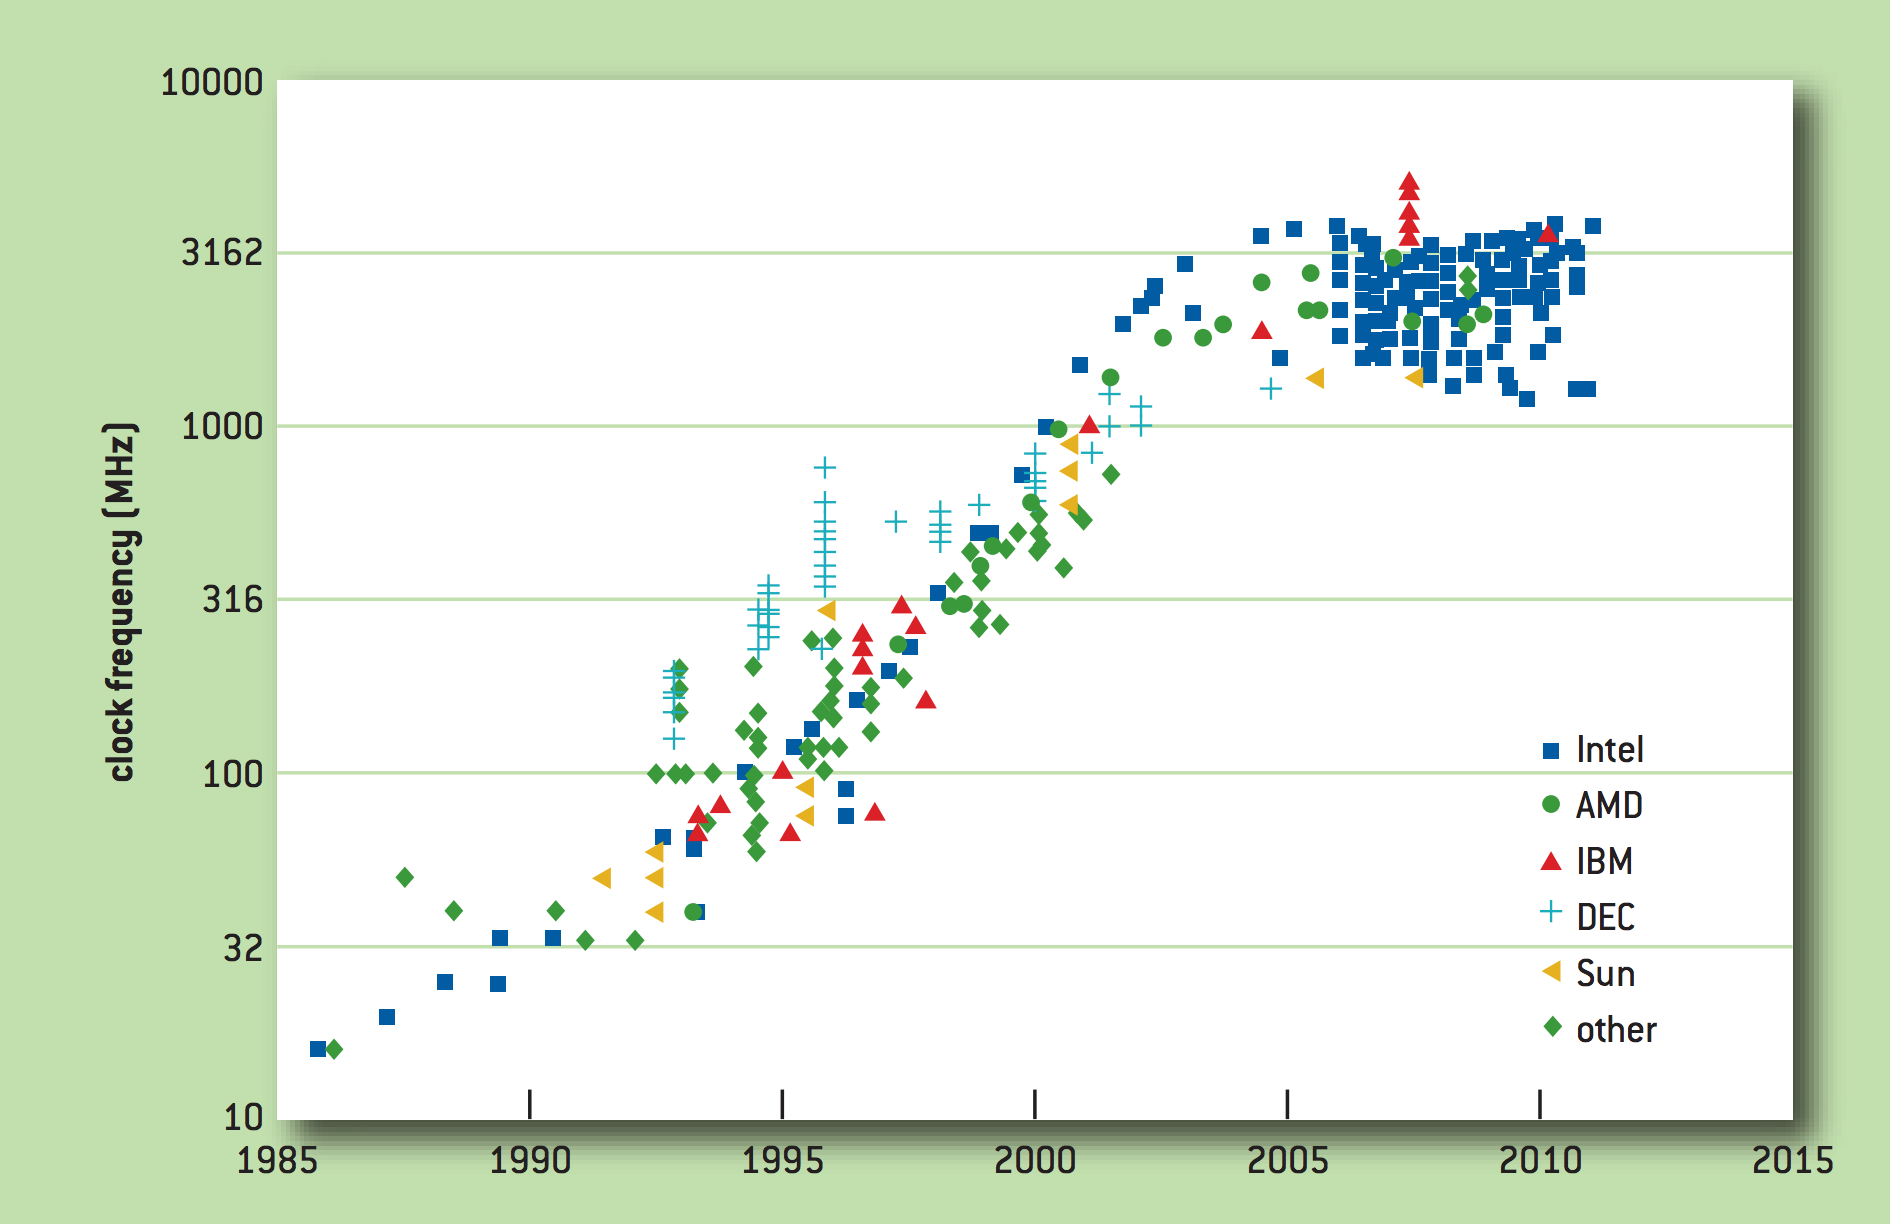
\includegraphics[width=0.7\textwidth]{images/cpu-frequency}
\end{center}

Clearly there is an area in which frequency scaling was effective. Next year's CPU would have a higher clock speed, and higher clock speed means more cycles per second, and more cycles per second means more work is done in a given second, and that means better performance. Except, we hit the wall: clock speeds stop getting faster around 2005, stopping at around 3 GHz. Speeding them up beyond this would take, well, more voltage which means more power and more heat, and more heat means higher failure/error rates, and more cooling, and the cooling takes power too, and all that waste heat, well, it will eventually, at the end of this chain, make polar bears sad.

Digression: if we look at the x86 processor, one with which everyone is probably at least \textit{passingly} familiar, it is a Complex Instruction Set Computing (CISC) processor. In other words, there are a lot of assembly instructions. But why? This was intended for your convenience as a programmer: if you were going to write assembly, wouldn't it be nice to have a sine function that takes one argument instead of having to grind out (or copy-paste) the calculation of a sine routine every single time you needed it? So the hardware people thought they were doing everyone a favour. These are easy to program in, from the way the assembly programmer thinks, but hard to implement and hard to pipeline. 

For a lot of CISC machines, the Cycles Per Instruction (CPI) varied, something like 4-10 cycles to complete any instruction, but at least it was predictable. Every time, no matter what, it takes the same number of cycles. Program performance was basically the number of page faults (disk accesses) times the amount of time it takes to read from disk, plus the instruction execution time (which is generally small compared to page fault service times)\footnote{For further discussion about this, see the ECE~254 notes about page faults and caching and disk read times.}. Thus the optimization goal is: minimize page faults. Page fault count is relatively easy to measure and there are some things we can do to reduce the number of page faults; optimize our data access patterns, change how we pack the data, et cetera. If you were working with an embedded system with no disk (or at least no page faults) then the optimization goal is minimize instruction count.

Between 1990 and 2005 we got some really impressive scaling on CPU frequency. This was caused by a few factors. The first is the advent of the Reduced Instruction Set Computing (RISC) CPU: simpler processors are easier to scale than complex ones, and simpler instructions mean fewer cycles per instruction. That also means we can have more pipelining. The tradeoff is that RISC CPUs are much harder to program in assembly directly, so compilers had to do the work. The example in~\cite{modern-hardware} is delay slots: an instruction after a branch is always executed or worse, the result of a computation is not available to the next instruction. In these cases the ``simple'' solution is to put a \texttt{NOP} (do-nothing) instruction in, good compilers (and programmers) can rearrange instructions, hopefully, to make this work without wasting time. And another thing: memory got cheaper, so we have more of it, so page faults occurred less and less frequently and that's really something.

But then, as we have seen, we hit the (power) wall. And you might think, well, if I run into a wall, I can just go around it. There must be other ways to advance! And there are, except, we hit three other walls too, and now we are surrounded\footnote{``He is intelligent, but not experienced. His pattern indicates two dimensional thinking.'' - Spock, \textit{Star Trek II: The Wrath of Khan}}. What are these other three seemingly-insurmountable barriers?

The first is instruction level parallelism (ILP) is getting close to the limit of what we can do. We can predict branches with a certain accuracy but if we have already got 95\% efficiency, no matter how much time and effort and money is invested into improving the branch prediction routine we get maximally a 5\% increase in branch prediction accuracy which translates into a very small speedup to the execution when we consider just how often a misprediction is the cause of the problem (5\% of 5\% is very small\ldots just making up numbers).

The speed of memory advances has not at all kept up with the advances in CPU technology, so now we have moved from the era of runtime being dominated by page faults to the era of runtime being dominated by cache misses. Adding more cache isn't a perfect solution though, and doubling, say, level one cache (at great expense) does not double the speed of the program; it may speed it up by a small amount at most. 

The final wall is the universal speed limit: the speed of light (curse you Einstein!). The more complex the CPU is, the longer the path any signal may have to travel to get from A to B. This is limited, most practically, by the speed of light, and thus far, nobody has invented a way to get around this universal speed limit (but we are working on it, and according to Star Trek, should have this sorted out by 2063 or so).

But let's go back to the subject of ILP. Branch prediction and pipelining have been touched upon but there is so much more to it. The idea with ILP is not having more cycles to work with, but instead, doing more in each clock cycle. And there's a lot of clever ideas. 

Pipelining: you may have heard a bit about this already, especially so if you have taken a CPU architecture course. To complete an instruction there are five basic steps: (1) fetch the instruction from memory, (2) decode the instruction, (3) fetch needed operands, (4) perform the operation, and (5) write the result. So to do an instruction like \texttt{ADD R1, R2}, we need to fetch the instruction, decode it and figure out what is to be done, read the values from \texttt{R1} and \texttt{R2}, do the addition, and then write the result to \texttt{R1}. Thus even a simple instruction takes more than one clock cycle, but the good news is that the stages can overlap:

\begin{center}
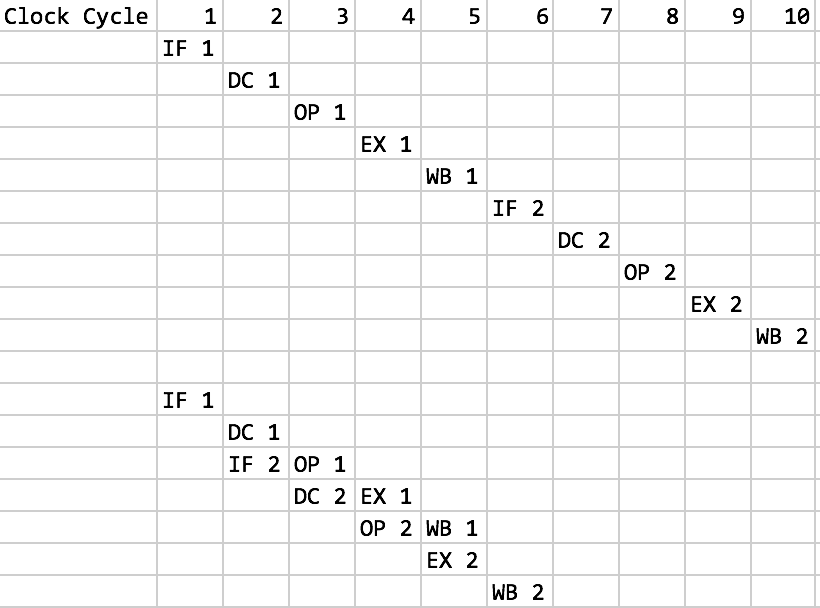
\includegraphics[width=0.4\textwidth]{images/pipelining}
\end{center}

In the above image, two instructions are shown. The top part shows no pipelining; the bottom shows what happens when pipelining is used. Each part of the instruction must be done sequentially---the instruction cannot be decoded until it is fetched---but at least the next instruction can be done. So it allows each of these to appear as if it is 1 clock cycle. If all goes well, then you complete one instruction per clock cycle. 

But there are pipeline hazards: sometimes you need the result of a previous step before you can go on. These prevent us from reaching the theoretical maximum of one instruction completed per clock cycle. Needing a previous result is not the only kind of hazard, though; we may have conflicts over certain CPU resources (how many floating point units are there, after all\ldots?) or fetch may be unable to identify the next instruction because of a branch. In the worst case, if we have mispredicted a branch, we have to flush the pipeline: throw away the instructions fetched, decoded, operands prepared, et cetera, because we guessed wrong and started doing the wrong actions. In that case, some extra work was done that was not necessary\ldots

The next idea relates to getting items from memory. If we do a load from memory, and we are lucky, it is found in the fastest cache and is available in perhaps 2-3 clock cycles. If we must go to memory, it may be 200-300 cycles. If it is in level 2 or level 3 cache it will be somewhere in between. The key idea, though, is if we are trying to put something in register \texttt{R7}, it will take time until that value is actually present in that register. The simplest approach is to just wait around until that value has arrived, and then go on to the next instruction. That works, but we can do better.

That better idea is: continue executing until \texttt{R7} is used somewhere. This allows us to get some useful work done in the meantime. Hardware keeps track of the fact that the register is not quite ready yet, but the work can get done in what is called the ``miss shadow''. It's possible to have more than one load in flight at a time. Two or more can be done in various CPU architectures, but it is of course hardware dependant. 

Branch prediction has come up already, but if we have a load followed by a compare used as a branch, we can then, well, guess. If we are wrong, there is the need to cleanup. But the good news is that branch prediction is usually right most of the time, perhaps 95\% or more (we'll definitely return to this later).

Another nice thing that the hardware can do for us is ``dual issue'' instructions. If we have two consecutive instructions that both take the same amount of time, use unrelated registers, and don't consume two of the same resource, we can start both instructions at once. If the instructions are \texttt{ADD R1, 16} and \texttt{CMP R2, 0} they do different things with different registers so there is no reason these cannot be done in parallel (if there are enough fetch/decode/etc units). In an embedded system, you may be interested in ensuring that this happens during a computationally intensive loop, such as encoding/decoding of media. If programmed correctly, you can be sure you get dual issue on every cycle.

Then a group of things that somewhat go together: register renaming, branch prediction, speculation, and Out-of-Order (O-O-O) Execution. These all work synergistically: each adds to the benefits the other brings. Register renaming works on a fairly simple principle: an assembly instruction says to read from register \texttt{R4}, but behind the scenes inside the processor, it is mapped to a physical register (let's say \texttt{RA} for the purpose of the example). Consider the following assembly instructions:

\begin{verbatim}
MOV R2, R7 + 32
ADD R1, R2
MOV R2, R9 + 64
ADD R3, R2
\end{verbatim}

Under normal circumstances, we cannot do instruction 3 until instruction 2 has been completed because we need the value of \texttt{R2} that was put in there (taken from memory somewhere) to be added to \texttt{R1}. Except, with register renaming, behind the scenes the first two instructions may replace \texttt{R2} with \texttt{RX} and the second pair of instructions have \texttt{R2} replaced with \texttt{RY} and these things can take place in parallel, or without a stall, at the very least.

This has a certain synergy with branch prediction. If we predict a branch, we can do speculative changes into one set of registers while we keep the ``old'' register values around too. When we figure out whether the branch prediction is correct, we can then get rid of the ones we don't need: the originals if predicted correctly, and the new values otherwise. So we get better recovery if there is a misprediction. Actually, I bet students wish they could do this: write down both answers to a question and let the TA pick the correct one at the end\ldots

Most importantly, it allows us to get past a cache miss and keep going; the goal here is to run until we can start the next cache miss, because the sooner that starts the sooner it's over, and the faster the program executes, ultimately. A quick example from the presentation demonstrates this, in x86 assembly~\cite{modern-hardware}:

\begin{verbatim}
ld rax, rbx+16   ; assume cache miss
add rbx, 16      ; carry on anyway, ADD doesn't need rax value from LD
                 ; register renaming => LD (write)/ADD (read) don't interfere
cmp rax, 0       ; needs rax value, queue till available
jeq null_chk     ; oops! need cmp result
                 ; speculate: assume branch not taken
st rbx-16, rcx   ; speculatively store to store buf (not L1)
ld rcx, rdx      ; unrelated cache miss: 2 misses now active, 1 speculative
ld rax, rax+8    ; now must wait for result of first LD
\end{verbatim}

%Let's assume \texttt{rax} (register A) is not available and the first instruction is a cache miss and it will take 300 cycles to get it. So we carry on. Then the instruction next is unrelated so we can go on. It doesn't matter that \texttt{rbx} is read in the first two instructions, because we can do register renaming so that internally it's reading from register 4 and writing to register 12. The compare cannot proceed because the first load's value is not available, but it will be queued up to be done later. Then we have a branch, but we don't know what the flags are, because we can't compare, because the load isn't done. The branch predictor will say in this example that we will not take the branch and go on to the store instruction (\texttt{st}). The store is speculative because the branch may have been taken (so it goes in a store buffer temporarily and not to L1 cache, until we are sure it's okay to let it go to memory). We have now made it to the second last line and we have another unrelated cache miss, and we have two cache misses running in parallel (the second of which is speculative). Finally, the last instruction has to wait for the first instruction to fill the register \texttt{rax} and we can no longer speculate.

To summarize: there are seven operations we were trying to do here with two cache misses. The cache misses complete in cycles 300 and 304 (maybe 302 if we have dual issue), so in total we complete 7 operations in about 305 cycles. All the trickery and cleverness got us to that second miss which means we complete in 305. If we did not manage that, it would take about 600 cycles to complete it all. So we did double performance, even though in this example our overall performance was terrible.
 
For years Intel was trying to push its Itanium processors (which were so unsuccessful they got the nickname ``Itanic''. Ouch). The goal of these was to find static (compile-time) parallelism: if a machine has infinite registers, can speculate infinitely, etc, the program gets sped up. Run all possibilities in parallel and at the end figure out which is right (wasn't this a Nicolas Cage movie?). Unfortunately it didn't work out very well because this requires the right kind of program and an super smart compiler. Oh yes, and infinite registers requires infinite space as well as infinite money. So instead the quest has turned to how we can get better performance out of x86\ldots

The x86 approach tries to maximize dynamic (run-time) parallelism. This has been done incrementally, with more pipelining, re-order buffers, adding more functional units, and so on. But the walls are still there: cache miss rates and branch mispredicts continue to dominate performance, even though the rates are very low, because a miss costs so much. 

How are we doing so far? Well, here's a short video that goes over where we were in the beginning of 2017: \url{https://www.youtube.com/watch?v=4A0Iks4ENIs} with the launch of Intel's latest (at the time) processor. But since then, AMD launched Ryzen---Never turn your back on Threadripper!---and it's forced Intel to compete again\ldots In 2020 the situation is more like \url{https://www.youtube.com/watch?v=a8apEJ5Zt2s}.

According to~\cite{modern-hardware} something like 90-99\% of the transistors on a modern x86 chip are spent in cache. In spite of the extreme complexity of the decode logic that allows multiple parallel decodes of all the weird and wacky instructions of the x86, pushing cache to the biggest size it can be is so important because it prevents the performance hit of going to memory.

The image below (from Sun World Wide Analyst Conference in 2003) is obviously a bit dated but this is very instructive as to the trend:
\begin{center}
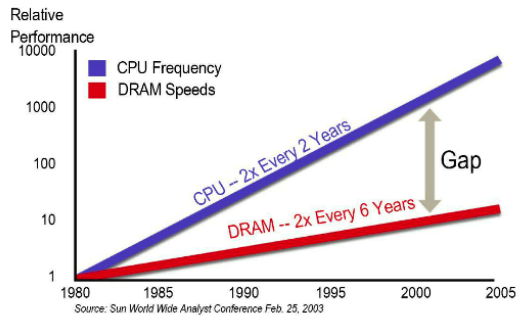
\includegraphics[width=0.6\textwidth]{images/ram-vs-cpu.png}
\end{center}

DRAM is, however, not the only kind of memory. There is SRAM (Static RAM) which is fast but expensive, the kind of stuff that goes on the CPU die, and it is six transistors per bit. Compare against DRAM which is much cheaper, but slow: one transistor and one capacitor per bit. Improvements in DRAM have not really improved latency but have improved bandwidth; DDR (Dual Data Rate\ldots not Dance Dance Revolution) means there are two transfers per cycle, but it still takes significant time to get any data out. And DRAM needs occasional refreshes (capacitors\ldots) so sometimes we have to wait for that.

In the Operating Systems course you probably learned that disk is the slowest thing and the limiting factor. That's true, as Obi-Wan Kenobi would say, from a certain point of view. Now that we live in the world of Solid State Drives (SSDs), ``disk'' reads are about as fast as memory reads and memory reads are the rate-limiting step in the system. Nonvolatile memory looks to be even faster. More is the new more, orange is the new black, and memory is the new disk.

To get memory access speed up there are things we can do, like relax coherency constraints, more synchronization through locks\ldots all of which we will come back to in some upcoming lectures. 

If we want to get better performance, we need to figure out where time is going. For that we will have the subject of profiling, which comes up in some later lectures. If we can track down where our cache misses are occurring, maybe, just maybe, we can do something about it. 

\section*{A Deeper Look at Cache Misses}

As discussed, the CPU generates a memory address for a read or write operation. The address will be mapped to a page. Ideally, the page is found in the cache, because that would be faster. If the requested page is, in fact,  in the cache, we call that a cache \textit{hit}. If the page is not found in the cache, it is considered a cache \textit{miss}. In case of a miss, we must load the page from memory, a comparatively slow operation. The percentage of the time that a page is found in the cache is called the \textit{hit ratio}, because it is how often we have a cache hit. We can calculate the effective access time if we have a good estimate of the hit ratio (which is not overly difficult to obtain) and some measurements of how long it takes to load data from the cache and how long from memory. The effective access time is therefore computed as:

\begin{center}
Effective Access Time = $h \times t_{c} + (1-h) \times t_{m}$
\end{center}

Where $h$ is the hit ratio, $t_{c}$ is the time required to load a page from cache, and $t_{m}$ is the time to load a page from memory. Of course, we would like the hit ratio to be as high as possible. 

Caches have limited size, because faster caches are more expensive. With infinite money we might put everything in registers, but that is rather unrealistic. Caches for memory are very often multileveled; Intel 64-bit CPUs tend to have L1, L2, and L3 caches. L1 is the smallest and L3 is the largest. Obviously, the effective access time formula needs to be updated and expanded when we have multiple levels of cache with different access times and hit rates. See the diagram below:

\begin{center}
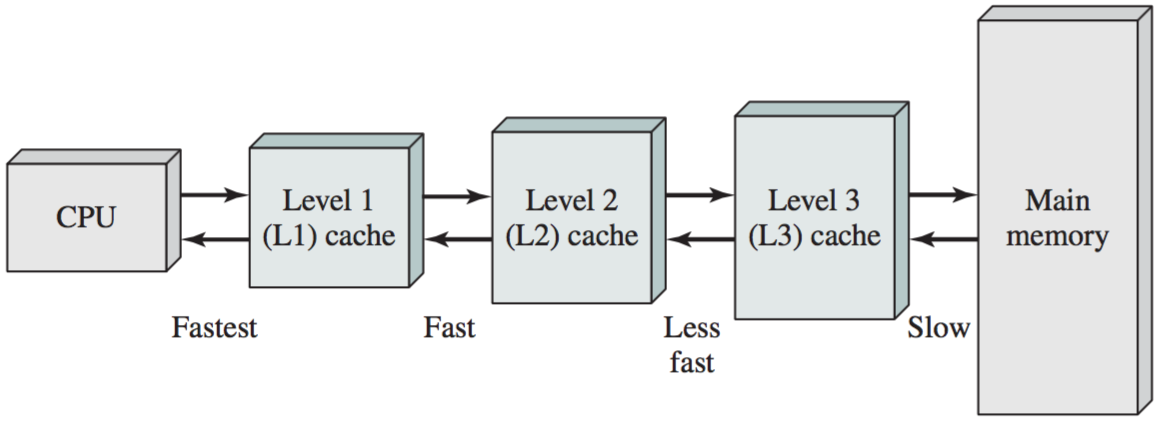
\includegraphics[width=0.6\textwidth]{images/caches.png}\\
Three levels of cache between the CPU and main memory~\cite{osi}.
\end{center}

If we have a miss in the L1 cache, the L2 cache is checked. If the L2 cache contains the desired page, it will be copied to the L1 cache and sent to the CPU. If it is not in L2, then L3 is checked. If it is not there either, it is in main memory and will be retrieved from there and copied to the in-between levels on its way to the CPU. 

Cliff Click said that 5\% miss rates dominate performance. Let's look at why.
I looked up a characterization of the SPEC CPU2000 and CPU2006 
benchmarks~\cite{cpu2006}.

Here are the reported cache miss rates\footnote{\permil~is ``permil'', or per-1000.} for SPEC CPU2006.

\begin{center}
\begin{tabular}{ll}
L1D & 40\permil \\
L2 & 4 \permil
\end{tabular}
\end{center}

Let's assume that the L1D cache miss penalty is 5 cycles and the L2 miss penalty is
300 cycles, as in the video. Then, for every instruction, you would expect a running
time of, on average:
\[ 1 + 0.04 \times 5 + 0.004 \times 300 = 2.4. \]
Misses are expensive!


If we replace the terms $t_{c}$ and $t_{m}$ with $t_{m}$ and $t_{d}$ (time to retrieve it from disk) respectively, and redefine $h$ as $p$, the chance that a page is in memory, we can get an idea of the effective access time in virtual memory: 

\begin{center}
	Effective Access Time = $ p \times t_{m} + (1 - p) \times t_{d}$
\end{center}

And just while we're at it, we can combine the caching and disk read formulae to get the true effective access time for a system where there is only one level of cache:

\begin{center}
	Effective Access Time = $ h \times t_{c} + (1 - h) ( p \times t_{m} + (1 - p) \times t_{d})$
\end{center}

This is good, but what is $t_{d}$? This is a measurable quantity so it is possible, of course, to just measure it\footnote{One of my favourite engineering sayings is ``Don't guess; measure.'' You may be sick of hearing me say that one by now.}.

The slow step in all of this, is obviously, the amount of time it takes to load the page from disk. According to~\cite{osc}, restarting the process and managing memory and such take something like 1 to 100~$\mu$s. A typical hard drive in their example has a latency of 3~ms, seek time (moving the read head of the disk to the location of the page) is around 5~ms, and a transfer time of 0.05~ms. So the latency plus seek time is the limiting component, and it's several orders of magnitude larger than any of the other costs in the system. And this is for servicing a request; don't forget that several requests may be queued, making the time even longer.

Thus the disk read term $t_{d}$ dominates the effective access time equation. If memory access takes 200~ns and a disk read 8~ms, we can roughly estimate the access time in nanoseconds as $(1-p) \times 8~000~000$. 

If the page fault rate is high, performance is awful. If performance of the computer is to be reasonable, the page fault rate has to be very, very low.

Summary: misses are not just expensive, they hurt performance more than anything else.










\chapter*{7 --- CPU Hardware, Branch Prediction}

\addcontentsline{toc}{chapter}{7 --- CPU Hardware, Branch Prediction}

\section*{Multicore Processors}
As I've alluded to earlier, multicore processors came about because
clock speeds just aren't going up anymore. We'll discuss technical
details today. Each processor \emph{core} executes instructions; a processor with more than one core can therefore simultaneously execute multiple
(unrelated) instructions. 

\paragraph{Chips and cores.} Multiprocessor (usually SMP, or symmetric
multiprocessor) systems have been around for a while. Such systems
contain more than one CPU. We can count the number of CPUs by
physically looking at the board; each CPU is a discrete physical thing.

Cores, on the other hand, are harder to count. In fact, they look just
like distinct CPUs to the operating system:

{\scriptsize \begin{verbatim}
plam@plym:~/courses/p4p/lectures$ cat /proc/cpuinfo
processor	: 0
vendor_id	: GenuineIntel
cpu family	: 6
model		: 23
model name	: Pentium(R) Dual-Core  CPU      E6300  @ 2.80GHz
...
processor	: 1
vendor_id	: GenuineIntel
cpu family	: 6
model		: 23
model name	: Pentium(R) Dual-Core  CPU      E6300  @ 2.80GHz
\end{verbatim}
}
\vspace*{-1em}
%$ 
If you actually opened my computer, though, you'd only find one chip.
The chip is pretending to have two \emph{virtual CPUs}, and the
operating system can schedule work on each of these CPUs. In general,
you can't look at the chip and figure out how many cores it contains.

\vspace*{-1em}
\paragraph{Hardware Designs for Multicores.}
In terms of the hardware design, cores might share a cache, as in this picture:

\vspace*{-1em}
\begin{center}
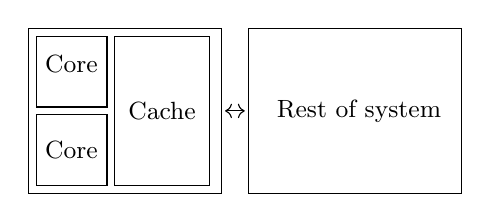
\begin{tikzpicture}
\draw (-0.5, -0.5) rectangle ++(0.9, 0.9);
\draw (-0.05, 0.05) node {\small Core};

\draw (-0.5, -1.5) rectangle ++(0.9, 0.9);
\draw (-0.05, -1.05) node {\small Core};

\draw (0.5, -1.5) rectangle ++(1.2, 1.9);
\draw (1.1, -.55) node {\small Cache};

\draw (-0.6, -1.6) rectangle ++(2.45, 2.1);

\draw (2.2, -1.6) rectangle ++(2.7, 2.1);
\draw (3.6, -0.55) node {\small Rest of system};

\draw[<->] (1.9, -0.55) -- (2.15, -0.55);
\end{tikzpicture}
\end{center}
\vspace*{-1em}
\hfill (credit: \emph{Multicore Application Programming}, p. 5)

This above Symmetric Multithreading (SMP) design is especially good for the 1:1 threading model. In
this case, the design of the cores don't need to change much, but they
still need to communicate with each other and the rest of the system.

Or, we can have a design that works well for the N:1 model:
\begin{center}
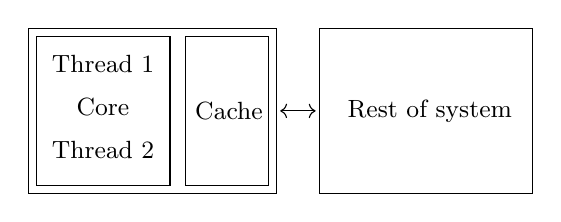
\begin{tikzpicture}
\draw (-1.4, -1.5) rectangle ++(1.7, 1.9);
\draw (-0.55, 0.05) node {\small Thread 1};
\draw (-0.55, -1.05) node {\small Thread 2};
\draw (-0.55, -0.5) node {\small Core};

\draw (0.5, -1.5) rectangle ++(1.05, 1.9);
\draw (1.05, -.55) node {\small Cache};

\draw (-1.5, -1.6) rectangle ++(3.15, 2.1);

\draw (2.2, -1.6) rectangle ++(2.7, 2.1);
\draw (3.6, -0.55) node {\small Rest of system};

\draw[<->] (1.7, -0.55) -- (2.15, -0.55);
\end{tikzpicture}
\end{center}

One would expect that executing two threads on one core might
mean that each thread would run more slowly. It depends on the instruction
mix. If the threads are trying to access the same resource, then each
thread would run more slowly. If they're doing different things, there's 
potential for speedup.

Finally, it's possible to both use multiple cores and put multiple threads
onto one core, as in the M:N model:

\begin{center}
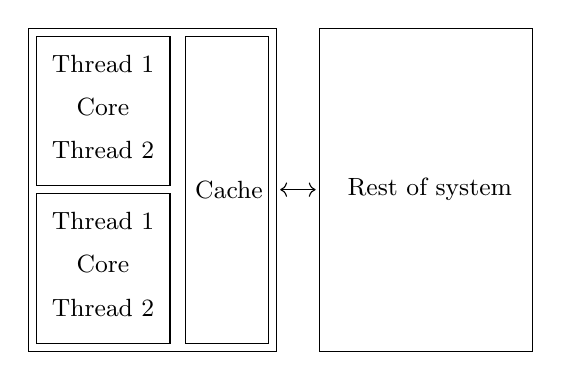
\begin{tikzpicture}

 \draw (-1.4, -1.5) rectangle +(1.7, 1.9);
 \draw (-1.4, -3.5) rectangle +(1.7, 1.9);

\foreach \y in {-2, 0}
{
 \draw (-0.55, 0.05) + (0, \y) node {\small Thread 1};
 \draw (-0.55, -1.05) + (0, \y) node {\small Thread 2};
 \draw (-0.55, -0.5) + (0, \y) node {\small Core};
}

\draw (0.5, -3.5) rectangle ++(1.05, 3.9);
\draw (1.05, -1.55) node {\small Cache};

\draw (-1.5, -3.6) rectangle ++(3.15, 4.1);

\draw (2.2, -3.6) rectangle ++(2.7, 4.1);
\draw (3.6, -1.55) node {\small Rest of system};

\draw[<->] (1.7, -1.55) -- (2.15, -1.55);
\end{tikzpicture}
\end{center}
Here we have four hardware threads; pairs of threads share hardware
resources. One example of a processor which supports chip multi-threading
(CMT) is the UltraSPARC T2, which has 8 cores, each of which supports 8 
threads. All of the cores share a common level 2 cache.

\paragraph{Non-SMP systems.} The designs we've seen above have been
more or less SMP designs; all of the cores are mostly alike.
A very non-SMP system is the Cell, which contains a PowerPC main core
(the PPE) and 7 Synergistic Processing Elements (SPEs), which are
small vector computers.


\paragraph{Non-Uniform Memory Access.}
In SMP systems, all CPUs have approximately the same access time for resources
(subject to cache misses). There are also NUMA, or Non-Uniform Memory Access,
systems out there. In that case, CPUs can access different resources at different
speeds. (Resources goes beyond just memory).

In this case, the operating system should schedule tasks on CPUs which
can access resources faster.  Since memory is commonly the bottleneck,
each CPU has its own memory bank.

\paragraph{Using CMT effectively.} Typically, a CPU will expose its
hardware threads using virtual CPUs.
In current hardware designs, each of the hardware threads has the same
performance. 

However, performance varies depending on context. In the above
example, two threads running on the same core will most probably run
more slowly than two threads running on separate cores, since they'd
contend for the same core's resources. Task switches between cores (or
CPUs!) are also slow, as they may involve reloading caches.

Solaris ``processor sets''
enable the operating system to assign processes to specific virtual CPUs,
while Linux's ``affinity'' keeps a process running on the same virtual CPU.
Both of these features reduce the number of task switches, and processor
sets can help reduce resource contention, along with Solaris's locality
groups.\footnote{Gove suggests that locality groups help reduce contention
for core resources, but they seem to help more with memory.}



\section*{Branch Prediction and Misprediction}

The compiler (and the CPU) take a look at code that results in branch instructions  such as loops, conditionals, or the dreaded \texttt{goto}\footnote{Which I still maintain is a swear word in C.}, and it will take an assessment of what it thinks is likely to happen. By default I think it's assumed that backward branches are taken and forward branches are not taken (but that may be wrong).  Well, how did we get here anyway?

In the beginning the CPUs and compilers didn't really think about this sort of thing, they would just come across instructions one at a time and do them and that was that. If one of them required a branch, it was no real issue. Then we had pipelining: the CPU would fetch the next instruction while decoding the previous one, and while executing the instruction before. That means if evaluation of an instruction results in a branch, we might go somewhere else and therefore throw away the contents of the pipeline. Thus we'd have wasted some time and effort. If the pipeline is short, this is not very expensive. But pipelines keep getting longer\ldots

So then we got to the subject of branch prediction. The compiler and CPU look at instructions on their way to be executed and analyze whether it thinks it's likely the branch is taken. This can be based on several things, including the recent execution history. If we guess correctly, this is great, because it minimizes the cost of the branch. If we guess wrong, we have to flush the pipeline and take the performance penalty.

The compiler and CPU's branch prediction routines are pretty smart. Trying to outsmart them isn't necessarily a good idea. It's possible to give \texttt{gcc} some hints: we say either something is likely or unlikely. 

 These hints tell the compiler some information about how it should predict. It will then arrange the instructions in such a way that, if the prediction is right, the instructions in the pipeline will be executed. But if we're wrong, then the instructions will have to be flushed.

From what I can tell, the core Rust team isn't super comfortable with the idea of exposing these kinds of internal-compiler things, but there is an implementation of the likely/unlikely concept. You can sort of use it, but it could break in the future, as an experimental feature. If you want the experimental features enabled, you have to be using nightly build of Rust and to specify the feature at the top of your source file (e.g., \texttt{\#![feature(core\_intrinsics)]})

Do they work? Here's a sample program to find out. I'll first test it with no hint, then putting \texttt{likely()} around the if condition, and then \texttt{unlikely()}, and show you the results.

\begin{lstlisting}[language=Rust]
fn f(a: i32) -> i32 {
    a
}

fn main() {
    let size = 100000;
    let large_vector = vec![0; size];
    let mut m1 = 0;
    let mut m2 = 0;

    for _j in 0..1000 {
        for k in 0..size {
            if *large_vector.get(k).unwrap() == 0 {
                m1 = f(m1 + 1)
            } else {
                m2 = f(m2 + 1)
            }
        }
    }
    println!("m1 = {}; m2 = {}", m1, m2);
}
\end{lstlisting}

And the results:
\begin{verbatim}
No hint at all:
  Time (mean +/- ?):      6.657 s +/-  0.144 s    [User: 6.614 s, System: 0.029 s]
  Range (min ... max):    6.413 s ...  6.905 s    10 runs
  
Likely:
  Time (mean +/- ?):      6.762 s +/-  0.175 s    [User: 6.729 s, System: 0.028 s]
  Range (min ... max):    6.590 s ...  7.200 s    10 runs

Unlikely:
  Time (mean +/- ?):      6.943 s +/-  0.200 s    [User: 6.893 s, System: 0.033 s]
  Range (min ... max):    6.732 s ...  7.309 s    10 runs
\end{verbatim}

Looks like hints don't help very much in this program at all. They made it marginally worse, not better. And getting it wrong comes with a penalty, too. This program might not be the ideal test case for hints, in that there might be a different scenario where the hints have a positive impact. However, we have at least established that hints aren't always a benefit, even if we know we're right. Under a lot of circumstances then, it's probably best just to leave it alone, unless we're really, really, really sure. 

Conclusion: it's hard to outsmart the compiler. Maybe it's better not to try.

\subsection*{How does branch prediction work, anyway?}
We can write software. The hardware will make it fast. If we understand the hardware, we can understand when it has trouble making our software fast.

You've seen how branch prediction works in ECE 222. However, we'll talk about it today in the context of performance. Notes based on a transcript of a talk by Dan Luu~\cite{branchprediction}.

I want you to pick up two points from this discussion:
\vspace*{-1em}
\begin{itemize}[noitemsep]
\item how branch predictors work---this helps you understand some of the apparent randomness in your
execution times, and possibly helps you make your code more predictable; and,
\item applying a (straightforward) expected value computation to predict performance.
\end{itemize}

Let's consider the following assembly code:

\hspace*{2em} \begin{minipage}{.4\textwidth} \begin{lstlisting}
branch_if_not_equal x, 0, else_label
// Do stuff
goto end_label
else_label:
// Do things
end_label:
// whatever happens later
\end{lstlisting}
\end{minipage}

The {\tt branch} instruction may be followed by either ``stuff'' or ``things''.
The pipeline needs to know what the next instruction is, for instance to fetch it.
But it can't know the next instruction until it almost finishes executing the branch.
Let's look at some pictures, assuming a 2-stage pipeline.

With no prediction, we need to serialize:

\begin{center}
\begin{tabular}{c|c|c|c}
bne.1 & bne.2 \\ \hline
& & things.1 & things.2
\end{tabular}
\end{center}

\begin{minipage}{.49\textwidth}
Let's predict that ``things'' gets taken.
If our prediction is correct, we save time.

\begin{center}
\begin{tabular}{c|c|c}
bne.1 & bne.2 \\ \hline
& things.1 & things.2 \\
\\
\end{tabular}
\end{center}
\end{minipage} \hspace*{.02\textwidth} \begin{minipage}{.49\textwidth}
But we might be wrong and need to throw out the bad prediction.

\begin{center}
\begin{tabular}{c|c|c|c}
bne.1 & bne.2 \\ \cline{1-2}
& \sout{things.1} \\ \hline
& & stuff.1 & stuff.2
\end{tabular}
\end{center}
\end{minipage}

\paragraph{Cartoon model.} We need to quantify the performance.
For the purpose of this lecture, let's pretend that our pipelined
CPU executes, on average, one instruction per clock;
mispredicted branches cost 20 cycles, while correctly-predicted
branches cost 1 cycle. We'll also assume that the instruction
mix contains 80\% non-branches and 20\% branches. So we can predict
average cycles per instruction.

With no prediction (or always-wrong prediction):
\[
\mathrm{non\_branch\_\%} \times 1 \mathrm{~cycle} + \mathrm{branch\_\%} \times 20 \mathrm{~cycles} = 4.8 \mathrm{~cycles}.
\]
With perfect branch prediction:
\[
\mathrm{non\_branch\_\%} \times 1 \mathrm{~cycle} + \mathrm{branch\_\%} \times 1 \mathrm{~cycle} = 1 \mathrm{~cycle}.
\]
So we can make our code run 4.8$\times$ faster with branch prediction!

\paragraph{Predict taken.} What's the simplest possible thing? We can
predict that a branch is always taken. (Loop branches, for instance,
account for many of the branches in an execution, and are often taken.)
If we got 70\% accuracy, then our cycles per instruction would be:
\[
(0.8 + 0.7 \times 0.2) \times 1 \mathrm{~cycle} + (0.3 \times 0.2) \times 20 \mathrm{~cycles} = 2.14 \mathrm{~cycles}.
\]
The simplest possible thing already greatly improves the CPU's average throughput.

\paragraph{Backwards taken, forwards not taken (BTFNT).}
Let's leverage that observation about loop branches to do better.
Loop branches are, by definition, backwards (go back to previous
code). So we can design a branch predictor which predicts ``taken''
for backwards and ``not taken'' for forwards. The compiler can then
use this information to encode what it thinks about forwards branches
(that is, making the not-taken branch the one it thinks is more likely).
Let's say that this might get us to 80\% accuracy. \[
(0.8 + 0.8 \times 0.2) \times 1 \mathrm{~cycle} + (0.2 \times 0.2) \times 20 \mathrm{~cycles} = 1.76 \mathrm{~cycles}.
\]
The PPC 601 (1993) and 603 used this scheme.

\paragraph{Going dynamic: using history for branch prediction.}
So far, we will always make the same prediction at each branch---known as a
\emph{static} scheme. But we can do better by using what recently happened to
improve our predictions. This is particularly important when program execution
contains distinct phases, with distinct behaviours.
We therefore move to \emph{dynamic} schemes.

Once again, let's start with the simplest possible thing. For every branch,
we record whether it was taken or not last time it executed (a 1-bit scheme).
Of course, we can't store all branches. So let's use the low 6 bits of the address
to identify branches. Doing so raises the prospect of \emph{aliasing}:
different branches (with different behaviour) map to the same spot in the table.

We might get 85\% accuracy with such a scheme.
\[
(0.8 + 0.85 \times 0.2) \times 1 \mathrm{~cycle} + (0.15 \times 0.2) \times 20 \mathrm{~cycles} = 1.57 \mathrm{~cycles}.
\]

At the cost of more hardware, we get noticeable performance improvements. The DEC EV4 (1992) and
MIPS R8000 (1994) used this one-bit scheme.

\paragraph{Two-bit schemes.}
What if a branch is almost always taken but occasionally not taken (e.g. TTTTTTNTTTT)?
We get penalized twice
for that misprediction: once when we mispredict the not taken, and once when we mispredict the
next taken. So, let's store whether a branch is ``usually'' taken, using a so-called
2-bit saturating counter.

Every time we see a taken branch, we increment the counter for that
branch; every time we see a not-taken branch, we decrement. Saturating
means that we don't overflow or underflow. We instead stay at 11 or
00, respectively.

If the counter is 00 or 01, we predict ``not taken''; if it is 10 or
11, we predict ``taken''.

With a two-bit counter, we can have fewer entries at the same size, but they'll do better.
It would be reasonable to expect 90\% accuracy.
\[
(0.8 + 0.9 \times 0.2) \times 1 \mathrm{~cycle} + (0.1 \times 0.2) \times 20 \mathrm{~cycles} = 1.38 \mathrm{~cycles}.
\]

This was used in a number of chips, from the LLNL S-1 (1977) through the Intel Pentium (1993).

\paragraph{Two-level adaptive, global.}
We're still not taking patterns into account. Consider the following {\tt for} loop.
\begin{lstlisting}[language=C]
for (int i = 0; i < 3; ++i) {
  // code
}
\end{lstlisting}
The last three executions of the branch determine the next direction:
\begin{verbatim}
 TTT => N
 TTN => T
 TNT => T
 NTT => T
\end{verbatim}
Let's store what happened the last few times we were at a particular address---the
\emph{branch history}. From a branch address and history, we derive an index, which
points to a table of 2-bit saturating counters. What's changed from the two-bit scheme
is that the history helps determine the index and hence the prediction.

After we take a branch, we add its direction to the history, so that the next lookup
maps to a different table entry.

This scheme might give something like 93\% accuracy.
\[
(0.8 + 0.93 \times 0.2) \times 1 \mathrm{~cycle} + (0.07 \times 0.2) \times 20 \mathrm{~cycles} = 1.27 \mathrm{~cycles}.
\]

The Pentium MMX (1996) used a 4-bit global branch history.

\paragraph{Two-level adaptive, local.}
The change here is that the CPU keeps a separate history for each branch.
So the branch address determines which branch history gets used.
We concatenate the address and history to get the index, which then points to a
2-bit counter again. We are starting to encounter diminishing returns, but we might
get 94\% accuracy:
\[
(0.8 + 0.94 \times 0.2) \times 1 \mathrm{~cycle} + (0.06 \times 0.2) \times 20 \mathrm{~cycles} = 1.23 \mathrm{~cycles}.
\]

The Pentium Pro (1996), Pentium II (1997) and Pentium III (1999) use this.

\paragraph{gshare.}
Instead of concatenating the address and history, we can xor them. This allows
us to use more bits for both the history and address. This keeps the accuracy the same,
but simplifies the design.

\paragraph{Other predictors.} We can build (and people have built) more sophisticated predictors.
These predictors could, for instance, better handle aliasing, where
different branches/histories map to the same index in the table. But we'll stop here.

\paragraph{Summary of branch prediction.} We can summarize as follows.
Branch prediction enables pipelining and hence increased performance.
We can create a model to estimate just how critical branch prediction
is for modern processors. Fortunately, most branches are predictable
now. Aliasing (multiple branches mapping to the same entry in a
prediction table) can be a problem, but processors are pretty good at
dealing with that too.

\section*{Side-channel attacks}
There's been a lot happening lately in terms of exploiting the hardware of CPU architectures to get access to privileged data, and unfortunately these things have performance implications!

\subsection*{Cache Attacks}
In early 2018, the Spectre~\cite{Kocher2018spectre} and Meltdown~\cite{Lipp2018meltdown} attacks were disclosed. These attacks leverage performance features of modern CPUs to break process isolation guarantees---in principle, a process shouldn't be able to read memory that belongs to the kernel or to other processes.

The concept of cache side-channel attacks has been known for a while. If an attacker can get some memory loaded into the cache, then it can extract that memory using a cache side-channel attack.

Spectre and Meltdown can cause privileged memory to be loaded into the cache, and then extracted using a cache side-channel attack. We'll talk about Spectre (variant 2), since it attacks branch prediction in particular. My explanation follows~\cite{masters18:_what_meltd_spect} by Jon Masters of RedHat. However, you should now have enough background to follow the Google Project Zero description at~\cite{horn18:_readin}.

We know that at a branch, the CPU will start speculatively executing code at the inferred target of the branch. To exploit this vulnerability, the attack code convinces the CPU to speculatively execute code of its choice. The speculatively-executed attack code reads secret data (e.g. from the hypervisor kernel) and puts it in the cache. Once the data is in the cache, the attack proceeds by extracting the data from the cache.

Unfortunately, the only mitigation thus far involved additional security measures (in hardware and software) that unfortunately result in lower performance in program execution.

\subsection*{Hyperthreading attacks}
Multiprocessor (multicore) processors have some hardware that tries to keep the data consistent between different pipelines and caches (as we saw in the video). More processors, more threads means more work is necessary to keep these things in order. We will discuss cache coherence soon, but about hyperthreading... it turns out this is vulnerable too.

Remember that in hyperthreading, two threads are sharing the same execution core. That means they have hardware in common. Because of this, a thread can figure out what the other thread is doing by noticing its cache accesses and by timing how long it takes to complete operations. This is like sitting next to someone who's taking a multiple choice exam and noticing what answers they are choosing by how long it takes them to move their pencil down the page to fill in the correct circle. Yes, you have to be running on the same CPU as the victim, but still... Yikes! 

Researchers discovered and published a paper~\cite{portsmash} detailing the attack and showing a practical implementation of it. In the practical example, a 384-bit secret key is (over time) completely stolen by another process. It seems likely that this will lead in the long term to slowdowns of existing hardware as Operating System patches will need to prevent threads from different processes from using the same core... And possibly the only long term solution is to not use hyperthreading at all... the performance implications of which are both obvious and significant.









\chapter*{8 --- Cache Coherency}

\addcontentsline{toc}{chapter}{8 --- Cache Coherency}

\section*{Cache Coherency}

\begin{center}
    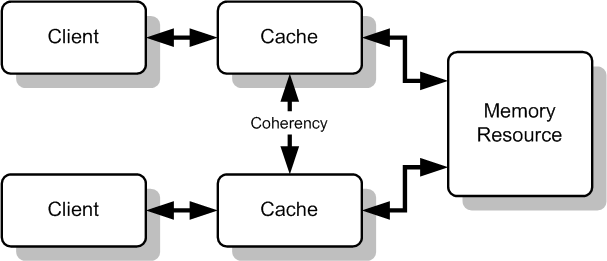
\includegraphics[width=0.5\textwidth]{images/coherency}

\hfill ---Wikipedia
\end{center}

Today we'll look at what support the architecture provides for memory ordering, in
particular in the form of cache coherence. Since this isn't an
architecture course, we'll look at this material more from the point
of view of a user, not an implementer.

The problem is, of course, that each CPU likely has its own cache. If it does, then the data in these may be out of sync---the value that CPU 1 has for a particular piece of data might be different from the value that CPU 4 has. The simplest method, and a horrible solution, would be the ability to declare some read/write variables as being non-cacheable (is that a word? Uncacheable?\ldots). The compiler and OS and such will require the data to be read from main memory, always. This will obviously result in lower cache hit ratios, increased bus traffic, and terrible, terrible performance. Let's avoid that. What we want instead is \textit{coherency}.

Cache coherency means that:
  \begin{itemize}
    \item the values in all caches are consistent; and
    \item to some extent, the system behaves as if all CPUs are using shared memory.
  \end{itemize}
  
In modern CPUs with three or four levels of cache, we frequently find that the level 3 cache isn't much faster than going to main memory. But this level is where the cache coherency communication can take place. This can be by making the cache shared between the different CPUs. And the L4 cache is frequently used for sharing data with the integrated graphics hardware on CPUs that have this feature. But for the most part we will imagine that caches are not shared, and we have to figure out how to get coherency between them. This is the case with a L1/L2 cache in a typical modern CPU as they are unique to the given core (i.e., not shared).
  
\paragraph{Cache Coherence Example.} We will use this example to illustrate
different cache coherence algorithms and how they handle the same situation.

Initially in main memory: {\tt x = 7}.

  \begin{enumerate}
    \item {\tt CPU1} reads x, puts the value in its cache.
    \item {\tt CPU3} reads x, puts the value in its cache.
    \item {\tt CPU3} modifies {\tt x := 42}
    \item {\tt CPU1} reads x \ldots ~from its cache?
    \item {\tt CPU2} reads x. Which value does it get?
  \end{enumerate}

Unless we do something, {\tt CPU1} is going to read invalid data.
  
Outside of a computing context, imagine you and several co-workers have some shared information, such as a meeting (in a specific room) in a shared online calendar (the one for the room). You (or anyone else) could make changes to this event. As mind-reading does not work, there are two ways that another invitee can know that something has changed: (1) they can check to see if anything has changed, or (2) they can be notified that a change has occurred. 

The notification may contain the updated information in its entirety, such as ``Event title changed to `Discuss User Permissions and Roles''', or it may just tell you ``something has changed; please check''. In transportation, you can experience both\ldots in the same day. I [JZ] was flying to Frankfurt and going to catch a train. Air Canada sent me an e-mail that said ``Departure time revised to 22:00'' (20 minute delay); when I landed the Deutsche Bahn (German railways) sent me an e-mail that said ``Something on your trip has changed; please check and see what it is in the app''\ldots it was my train being cancelled. I don't know why they couldn't have e-mailed me that in the first place! It's not like I was any less annoyed by finding out after taking a second step of opening an app.

Regardless of which method is chosen, we have to pick one. We can't pick none of those and expect to get the right answers.


\paragraph{Snoopy Caches.} The simplest way to ``do something''
is to use Snoopy caches~\cite{snoopycache}. No, not this kind of Snoopy (sadly):

\begin{center}
	
\includegraphics[width=0.3\textwidth]{images/peanuts-snoopy1.jpg}
\end{center}

It's called Snoopy because the caches are, in a way, spying on each other: they are observing what the other ones are doing. This way, they are kept up to date on what's happening and they know whether they need to do anything. They do not rely on being notified explicitly. This is a bit different from the transportation analogy, of course, but workable in a computer with a shared bus.

This is a distributed approach; no centralized state is maintained. Each cache with a copy of data from a block of main memory knows whether it is shared or not. All the CPUs are connected to a shared bus, and each CPU has its own cache controller. Whenever a CPU issues a memory write, the other CPUs are watching (colloquially, ``snooping around'') to observe if that memory location is in their cache. If so, the CPU will need to take action.

What does action mean? In the flight plus train example, both kinds of action occurred. The Air Canada action was \textit{update}---the information about the flight departure time was changed from 21:40 to 22:00 and at the time of becoming aware of the change, I got the new value immediately. The Deutsche Bahn action was \textit{invalidate}---the information about the train was changed, but I didn't know what had changed. All that I really knew is that the old information I had was out of date. When I needed that information again, I had to go get it myself from the source (their app). Either action (noting down the new, or knowing that what I have is out of date) is adequate for ensuring that I have the most up to date information. You may have a preference on which one you think is better, but unfortunately this is not your decision, neither as a user of the hardware of the computer nor as  a person who wants to travel by plane or train.

\subsection*{Write-Through Caches}
Let's put that into practice using write-through caches, the simplest type of
cache coherence.
  \begin{itemize}
    \item All cache writes are done to main memory.
    \item All cache writes also appear on the bus.
    \item If another CPU snoops and sees it has the same location in
      its cache, it will either invalidate or update the
      data.
  \end{itemize}
  
Invalidation is the most common protocol. It means the data in the cache of other CPUs is not updated, it's just noted as being out of date (invalid).  Normally, when you write to an invalidated location, you bypass the cache and go directly to memory (aka {\bf write no-allocate}). This kind of thing happens if you're just doing \texttt{x = 42;}---it doesn't matter what value of \texttt{x} was there before; you're just overwriting it.

If we want to do a read and there's a miss, we can ask around the other caches to see who has the most recent cached version. This is a bit like going into a room and yelling ``Does anybody have block\ldots?'', in some sort of multicast version of the card game ``Go Fish''. Regardless, the most recent value appears in memory, always, so if nobody else has it in cache (or they don't feel like sharing) you can get it from there.

There are also write broadcast protocols, in which case all versions in all caches get updated when there is a write to a shared block. But it uses lots of bandwidth and is not necessarily a good idea. It does, however prevent the costly cache miss that follows an invalidate. Sadly, as we are mere users and not hardware architects, we don't get to decide which is better; we just have to live with whichever one is on the hardware we get to use. Bummer.

\paragraph{Write-Through Protocol.}
The protocol for implementing such caches looks like this.
There are two possible states, {\bf valid} and {\bf invalid}, for each cached memory location.
Events are either from a processor ({\bf Pr}) or the {\bf Bus}. Actions will be either a \textbf{Rd} (read) or \textbf{Wr} (write).
We then implement the following state machine.

  \begin{center}
    \begin{tabular}{l|l|l|l}
      {\bf State} & {\bf Observed} & {\bf Generated} & {\bf Next State}\\ \hline
      Valid   & PrRd  &       & Valid\\
      Valid   & PrWr  & BusWr & Valid\\
      Valid   & BusWr &       & Invalid\\
      Invalid & PrWr  & BusWr & Valid\\
      Invalid & PrRd  & BusRd & Valid\\
    \end{tabular}
  \end{center}

\paragraph{Example.} For simplicity (this isn't an architecture course), assume all cache
      reads/writes are atomic. \footnote{If you're a hardware person, this line probably makes you cry. There's a whole lot that goes into making this work. There are potential write races, which have to be dealt with by contending for the bus and then completing the transaction, possibly restarting a command if necessary. If we have a split transaction bus it's really ugly, because we can have multiple interleaved misses. And down the rabbit hole we go.} Using the same example as before:

Initially in main memory: {\tt x = 7}.

  \begin{enumerate}
    \item {\tt CPU1} reads x, puts the value in its cache. {(valid)}
    \item {\tt CPU3} reads x, puts the value in its cache. {(valid)}
    \item {\tt CPU3} modifies {\tt x := 42}. {(write to memory)}
      \begin{itemize}
        \item {{\tt CPU1} snoops and marks data as invalid.}
      \end{itemize}
    \item {\tt CPU1} reads x, {from main memory. (valid)}
    \item {\tt CPU2} reads x, {from main memory. (valid)}
  \end{enumerate}

\subsection*{Write-Back Caches}
Let's try to improve performance. What if, in our example, {\tt CPU3} writes to {\tt x} 3 times in rapid succession? It's unpleasant to have to flush that to memory three times when we could do it only once. Let's try to delay the write to memory as long as possible. At minimum, we need support in hardware for a ``dirty'' bit, which indicates the our data has been changed but not yet been written to memory.

\paragraph{Write-Back Implementation.}
     The simplest type of write-back protocol (MSI) uses 3 states instead of 2:
      \begin{itemize}
        \item {\bf Modified}---only this cache has a valid copy; 
          main memory is {\bf out-of-date}.
        \item {\bf Shared}---location is unmodified, 
           up-to-date with main
          memory; 
          \quad may be present in other caches (also up-to-date).
        \item {\bf Invalid}---same as before.
      \end{itemize}
      
The initial state for a memory location, upon its first read, is ``shared''.
The implementation will only write the data to memory if another
processor requests it.
During write-back, a processor may read the data from the bus.

\paragraph{MSI Protocol.} Here, bus write-back (or flush) is {\bf BusWB}.
Exclusive read on the bus is {\bf BusRdX}.

\begin{center}
    \begin{tabular}{l|l|l|l}
      {\bf State} & {\bf Observed} & {\bf Generated} & {\bf Next State}\\ \hline
      Modified   & PrRd   &        & Modified\\
      Modified   & PrWr   &        & Modified\\
      Modified   & BusRd  & BusWB  & Shared\\
      Modified   & BusRdX & BusWB  & Invalid\\
      Shared     & PrRd   &        & Shared\\
      Shared     & BusRd  &        & Shared\\
      Shared     & BusRdX &        & Invalid\\
      Shared     & PrWr   & BusRdX & Modified\\
      Invalid    & PrRd   & BusRd  & Shared\\
      Invalid    & PrWr   & BusRdX & Modified\\
    \end{tabular}
\end{center}

\paragraph{MSI Example.} Using the same example as before:

Initially in main memory: {\tt x = 7}.

  \begin{enumerate}
    \item {\tt CPU1} reads x from memory. {(BusRd, shared)}
    \item {\tt CPU3} reads x from memory. {(BusRd, shared)}
    \item {\tt CPU3} modifies {\tt x = 42}:
      \begin{itemize}
        \item {Generates a BusRdX.}
        \item {{\tt CPU1} snoops and invalidates x.}
      \end{itemize}
    \item {\tt CPU1} reads x:
      \begin{itemize}
        \item {Generates a BusRd.}
        \item {{\tt CPU3} writes back the data and sets x to shared.}
        \item {{\tt CPU1} reads the new value from the bus as shared.}
      \end{itemize}
    \item {\tt CPU2} reads x from memory. {(BusRd, shared)}
  \end{enumerate}

\subsection*{An Extension to MSI: MESI}
    The most common protocol for cache coherence is MESI.
    This protocol adds yet another state:
      \begin{itemize}
        \item {\bf Modified}---only this cache has a valid copy; 
 main memory is {\bf out-of-date}.
        \item {\bf Exclusive}---only this cache has a valid copy; 
 main memory is {\bf up-to-date}.
        \item {\bf Shared}---same as before.
        \item {\bf Invalid}---same as before.
      \end{itemize}

    MESI allows a processor to modify data exclusive to it, without
    having to communicate with the bus.  MESI is safe. The key is that
    if memory is in the E state, no other processor has the data. The transition from E to M does not have to be reported over the bus, which potentially saves some work and reduces bus usage. 

\subsection*{MESIF: Even More States!}

    MESIF (used in latest i7 processors):
      \begin{itemize}
        \item {\bf Forward}---basically a shared state; but, current
          cache is the only one that will respond to a request to
          transfer the data.
      \end{itemize}

    Hence: a processor requesting data that is already shared or exclusive will
      only get one response transferring the data. Under a more simple MESI scheme you could get multiple caches trying to answer, with leads to bus arbitration or contention. The existence of a F state permits more efficient usage of the bus.
      
      
\subsection*{False Sharing}
False sharing is something that happens when our program has two unrelated data elements that are mapped to the same cache line/location. Let's consider an example from~\cite{falsesharing}:

\begin{lstlisting}[language=C]
char a[10];
char b[10];
\end{lstlisting}
These don't overlap but are almost certainly allocated next to each other in memory. If a thread is writing to \texttt{a} and they share a cache line, then \texttt{b} will be invalidated and the CPU working on \texttt{b} will be forced to fetch the newest value from memory. This can be avoided by seeing to it that there is some separation between these two arrays.

One way would be to heap allocate both arrays. You can find where things are located, if you are curious, by printing the pointer (or the address of a regular variable). Usually if you do this you will find that they are not both located at the same location. But you are provided no guarantee of that. So the other alternative is to make both arrays bigger than they need to be such that we're sure they don't overlap.

Consider the graph below that shows what happens in a sample program reading and writing these two arrays, as you increase the size of arrays \texttt{a} and \texttt{b} (noting that byte separation of 11 means they are adjacent; anything less than that and they overlap). This does waste space, but is it worth it?

\begin{center}
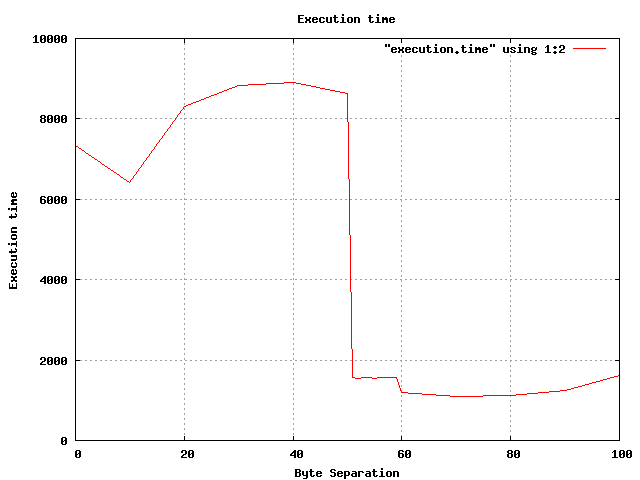
\includegraphics[width=0.6\textwidth]{images/falsesharing.png}\\
Execution time graph showing 5x speedup by ``wasting'' some space~\cite{falsesharing}.
\end{center}

At separation size 51 there is a huge drop in execution time because now we are certainly putting the two arrays in two locations that do not have the false sharing problem. Is wasting a little space worth it? Yes!

P.S. putting these arrays in a struct and padding the struct can also help with enabling future updates to the struct.









\chapter*{9 --- Concurrency and Parallelism}

\addcontentsline{toc}{chapter}{9 --- Concurrency and Parallelism}

\section*{Concurrency and Parallelism}
Concurrency and parallelism both give up the
total ordering between instructions in a sequential program, for
different purposes. We're going to focus on threads, but if you need a review of the details and differences of processes vs threads, you might like to read   \url{https://www.purplealienplanet.com/node/50}. 

\paragraph{Concurrency.} We'll refer to the use of threads for
structuring programs as concurrency. Here, we're not aiming
for increased performance. Instead, we're trying to write the program
in a natural way. Concurrency makes sense as a model for distributed
systems, or systems where multiple components interact, with no ordering
between these components, like graphical user interfaces.

\paragraph{Parallelism.} We're studying parallelism in this class, where
we try to do multiple things at the same time in an attempt to increase
throughput. Concurrent programs may be easier to parallelize.

\subsection*{Limits to parallelization}
I mentioned briefly in Lecture 1 that programs often have a sequential
part and a parallel part. We'll quantify this observation today
and discuss its consequences.

\paragraph{Scalable Algorithms.} 
Remember from ECE~250/CS~138 that we often care about the worst case run-time performance of the algorithm. A bad algorithm has terrible runtime characteristics for a large data set. Trying to do an insertion sort on a small array is fine (actually... recommended); doing it on a huge array is madness. Choosing a good algorithm is very important if we want it to scale.  But you know that already; you're not in a 4\textsuperscript{th} year engineering course to have me tell you that you can use quicksort rather than bubble sort.

\begin{center}
	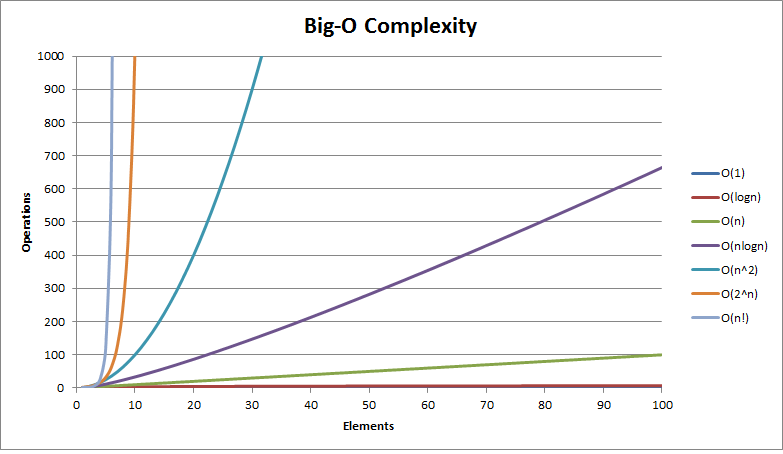
\includegraphics[width=0.75\textwidth]{images/big-o-complexity}\\
	Big-O Complexity comparison from ~\cite{bigocheatsheet}
\end{center}


\paragraph{Amdahl's Law.} One classic model of parallel execution
is Amdahl's Law. In 1967, Gene Amdahl argued that improvements in
processor design for single processors would be more effective than
designing multi-processor systems. Here's the argument. Let's say that
you are trying to run a task which has a serial part, taking fraction 
$S$, and a parallelizable part, taking fraction $P = 1-S$. Define $T_s$
to be the total 
amount of time needed on a single-processor system.
Now, moving to a parallel system with $N$ processors, the parallel
time $T_p$ is instead:
\[ T_p = T_s \cdot (S + \frac{P}{N}). \]
{\bf As $N$ increases, $T_p$ is dominated by $S$, limiting potential
speedup.}

We can restate this law in terms of speedup, which is the 
original time $T_s$ divided by the sped-up time $T_p$:
\[ \mbox{speedup} = \frac{T_s}{T_p} = \frac{1}{S+P/N}. \]
Replacing $S$ with $(1-P)$, we get:
\[ \mbox{speedup} = \frac{1}{(1-P)+P/N}, \]
and
\[ \mbox{max speedup} = \frac{1}{(1-P)}, \]
since $\frac{P}{N} \rightarrow 0$.

\paragraph{Plugging in numbers.} If $P = 1$, then we can indeed get good
scaling; running on an $N$-processor machine will give you a speedup
of $N$. Unfortunately, usually $P < 1$.  Let's see what happens.

\begin{center}
\begin{tabular}{r|r}
$P$ & speedup ($N=18$) \\ \hline
1 & 18 \\
0.99 & $\sim$ 15 \\
0.95 & $\sim$ 10 \\
0.5 & $\sim$ 2
\end{tabular}
\end{center}
Graphically, we have something like this:
\begin{center}
  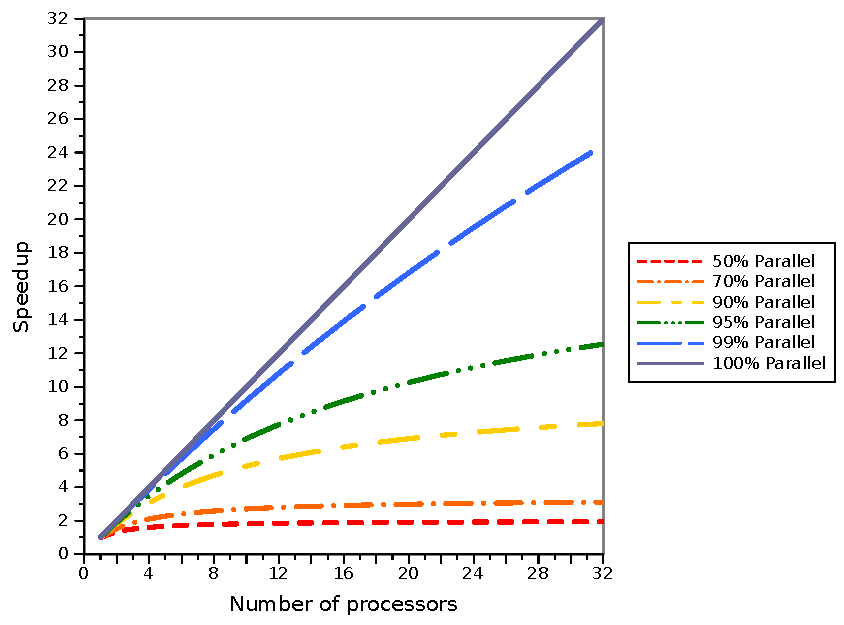
\includegraphics[width=0.5\textwidth]{images/parallel-scaling}
\end{center}


Amdahl's Law tells you how many cores you can hope to leverage in an
execution given a fixed problem size, if you can estimate $P$.

Let us consider an example from~\cite{mte241}: Suppose we have a task that can be executed in 5~s and this task contains a loop that can be parallelized. Let us also say initialization and recombination code in this routine requires 400~ms. So with one processor executing, it would take about 4.6~s to execute the loop. If we split it up and execute on two processors it will take about 2.3~s to execute the loop. Add to that the setup and cleanup time of 0.4~s and we get a total time of 2.7~s. Completing the task in 2.7~s rather than 5~s represents a speedup of about~46\%. Applying the formula, we get the following run times:

\begin{center}
	\begin{tabular}{l|l}
	\textbf{Processors} & \textbf{Run Time (s)} \\ \hline
	1 & 5\\
	2 & 2.7\\
	4 & 1.55\\
	8 & 0.975\\
	16 & 0.6875 \\
	32 & 0.54375 \\
	64 & 0.471875 \\
	128 & 0.4359375\\
	\end{tabular}
\end{center}

   \paragraph{Empirically estimating parallel speedup $P$.}
Assuming that you know things that are actually really hard to know, here's a formula for estimating speedup. You don't have to commit it to memory:
  \[P_{\mbox{\scriptsize estimated}} = \frac{\frac{1}{\mbox{\em speedup}}-1}{\frac{1}{N}-1}.\]

It's just an estimation, but you can use it to guess the fraction of parallel code, given $N$ and the speedup. You can then use $P_{\mbox{\scriptsize estimated}}$ to predict speedup for a different number of processors.

\paragraph{Consequences of Amdahl's Law.}
For over 30 years, most performance gains did indeed come from
increasing single-processor performance. The main reason that we're
here today is that, as we saw last time,
single-processor performance gains have hit the wall.

By the way, note that we didn't talk about the cost of synchronization
between threads here. That can drag the performance down even more.

\paragraph{Amdahl's Assumptions.}
Despite Amdahl's pessimism, we still all have multicore computers today.
Why is that? Amdahl's Law assumes that:
\begin{itemize}[noitemsep]
    \item problem size is fixed (read on);
    \item the program, or the underlying implementation, behaves the same on 1 processor as on $N$ processors; and
    \item that we can accurately measure runtimes---i.e. that overheads don't matter.
\end{itemize}

% replace Amdahl's law with how branch predictors work
\paragraph{Generalizing Amdahl's Law.} We made a simplification,
which was that programs only have one parallel part and one serial part.
Of course, this is not true. The program may have many parts,
 each of which we can tune to a different degree.

Let's generalize Amdahl's Law:

\begin{itemize}
\item  $f_1, f_2, \ldots, f_n$: fraction of time in part $n$
\item  $S_{f_1}, S_{f_n}, \ldots, S_{f_n}$: speedup for part $n$
\end{itemize}

Then,
\[\mbox{\em speedup} = \frac{1}{\frac{f_1}{S_{f_1}} + \frac{f_2}{S_{f_2}} + \ldots +
     \frac{f_n}{S_{f_n}}}.\]

\paragraph{Example.} Consider a program with 4 parts in the following scenario:

\begin{center}
     \begin{tabular}{r|r|r|r}
     \multicolumn{2}{l}{} & \multicolumn{2}{|c}{Speedup} \\
     Part & Fraction of Runtime & Option 1 & Option 2\\
     \hline
     1 & 0.55 & 1  & 2\\
     2 & 0.25 & 5  & 1\\
     3 & 0.15 & 3  & 1\\
     4 & 0.05  & 10 & 1\\
     \end{tabular}
 \end{center}

     (Note: these speedups don't have to be speedups from parallelization.)
    
   We can implement either Option 1 or Option 2. 
   Which option is better?

   ``Plug and chug'' the numbers:
 \begin{itemize}
 \item  {\bf Option 1.}

   \[ \mbox{\em speedup} = \frac{1}{0.55 + \frac{0.25}{5} + \frac{0.15}{3} + \frac{0.05}{5}}
     = 1.53  \]

 \item  {\bf Option 2.}

   \[\mbox{\em speedup} = \frac{1}{\frac{0.55}{2} + 0.45} = 1.38 \hspace*{5.5em}\]
\end{itemize}

\subsection*{A more optimistic point of view}
In 1988, John Gustafson pointed
out\footnote{\url{http://www.scl.ameslab.gov/Publications/Gus/AmdahlsLaw/Amdahls.html}}
that Amdahl's Law only applies to fixed-size problems, but that the
point of computers is to deal with bigger and bigger problems.

In particular, you might vary the input size, or the grid resolution,
number of timesteps, etc. When running the software, then, you might
need to hold the running time constant, not the problem size: you're
willing to wait, say, 10 hours for your task to finish, but not 500
hours. So you can change the question to: how big a problem can you
run in 10 hours?

According to Gustafson, scaling up the problem tends to increase the
amount of work in the parallel part of the code, while leaving the
serial part alone. As long as the algorithm is linear, it is possible
to handle linearly larger problems with a linearly larger number of
processors.

Of course, Gustafson's Law works when there is some ``problem-size''
knob you can crank up.  As a practical example, observe Google, which
deals with huge datasets.


\section*{Software Design Issues: Will it Parallelize?}


\paragraph{Locking and Synchronization Points.}
Think back to a concurrency course and the discussion of locking. We'll be coming back to this subject before too long. But for now, suffice it to say, that the more locks and locking we need, the less scalable the code is going to be. You may think of the lock as a resource and the more threads or processes that are looking to acquire that lock, the more ``resource contention'' we have, and the more waiting and coordination are going to be necessary. We're going to revisit the subject of wise use locks in more detail soon.

The previous paragraph applies as well to other concurrency constructs like semaphores, condition variables, etc. Any time a thread is forced to wait is going to be a limitation on the ability to parallelize the problem.

\paragraph{Memory Allocators.}
Assuming we're not working with an embedded system where all memory is statically allocated in advance, there will be dynamic memory allocation. The memory allocator is often centralized and may support only one thread allocating or deallocating at a time. This means it does not necessarily scale very well. There are, however, some techniques for dynamic memory allocation that allow these things to work in parallel.

\paragraph{Overhead.}
A first implementation might involve starting a thread for a task, then destroying it when it is complete. If there are many tasks and tasks are short-lived, then the fraction of time creating and destroying the threads may be significant.

 But that's not the only way. We can have a pool of workers. The workers are created once and only once. Then the application just submits units of work, and then on the other side these units of work are allocated to workers. The number of workers will scale based on the available hardware. This is neat as a programming practice: as the application developer we don't care quite so much about the underlying hardware. Let the operating system decide how many workers there should be, to figure out the optimal way to process the units of work.
 
Suppose you have to decide, though, how many threads should you create.
This depends
on which resources your threads use; if you are writing
computationally-intensive threads, then you probably want to have
fewer threads than the number of virtual CPUs. You can also use
Amdahl's Law to estimate the maximum useful number of threads, as
discussed previously.

Here's a longer discussion of thread pools:

\begin{center}
\url{http://www.ibm.com/developerworks/library/j-jtp0730.html}
\end{center}

Modern languages provide thread pools; Java's
\url{java.util.concurrent.ThreadPoolExecutor}~\cite{java:threadpoolexecutor}, C\#'s
\url{System.Threading.ThreadPool}~\cite{csharp:threadpool}, and GLib's {\tt GThreadPool}~\cite{gnome:threadpool} all implement thread pools. There's a Rust crate called \texttt{thread pool}. You can obviously write your own.

Here's a quick Rust program in which we use the threadpool crate to take away some of the complexity.
\begin{lstlisting}[language=Rust]
use std::collections::VecDeque;
use std::sync::{Arc, Mutex};
use threadpool::ThreadPool;
use std::thread;

fn main() {
    let pool = ThreadPool::new(8);
    let queue = Arc::new(Mutex::new(VecDeque::new()));
    println!("main thread has id {}", thread_id::get());

    for j in 0 .. 4000 {
        queue.lock().unwrap().push_back(j);
    }
    queue.lock().unwrap().push_back(-1);

    for i in 0 .. 4 {
        let queue_in_thread = queue.clone();
        pool.execute(move || {
            loop {
                let mut q = queue_in_thread.lock().unwrap();
                if !q.is_empty() {
                    let val = q.pop_front().unwrap();
                    if val == -1 {
                        q.push_back(-1);
                        println!("Thread {} got the signal to exit.", thread_id::get());
                        return;
                    }
                    println!("Thread {} got: {}!", thread_id::get(), val);
                }
            }
        });
    }
    pool.join();
}
\end{lstlisting}

It's important to note that when we call the \texttt{execute} function, that is a job to be run, so if our thread pool has four workers we want to push the consume ``job'' on it four times. They will then run and each will try to consume numbers until they get to the -1 answer which is the termination signal.

If we wrote our own implementation where we spawned the threads using the spawn mechanism, joining each thread individually might be a bit of a pain. 

This produces output that looks like:

\begin{verbatim}
main thread has id 4455538112
Thread 123145474433024 got: 0!
Thread 123145474433024 got: 1!
Thread 123145474433024 got: 2!

...

Thread 123145478651904 got: 3997!
Thread 123145478651904 got: 3998!
Thread 123145478651904 got: 3999!
Thread 123145476542464 got the signal to exit.
Thread 123145484980224 got the signal to exit.
Thread 123145474433024 got the signal to exit.
Thread 123145478651904 got the signal to exit.
\end{verbatim}

\paragraph{Threads and CPUs.} In your operating systems class,
you've seen implementations of threads (``lightweight processes'').
We'll call these threads \emph{software threads}, and we'll program
with them throughout the class. Each software thread corresponds to a
stream of instructions that the processor executes. On a old-school
single-core, single-processor machine, the operating system
multiplexes the CPU resources to execute multiple threads
concurrently; however, only one thread runs at a time on the single
CPU.

On the other hand, a modern chip contains a number of \emph{hardware
threads}, which correspond to the virtual CPUs. These are sometimes
known as \emph{strands}. The operating system still needs to 
multiplex the software threads onto the hardware threads, but now has
more than one hardware thread to schedule work onto.





\section*{Choose Your Pain}
The first design decision that you need to solve when parallelizing programs
is whether you should use threads or processes. Threads are basically light-weight processes which piggy-back on
          processes' address space.

\paragraph{When processes are better.} Processes are safer and more secure than threads.

  \begin{enumerate}
    \item Each process has its own virtual address space:
      \begin{itemize}
        \item Memory pages are not copied, they are copy-on-write (usually in UNIX, anyway). Therefore, processes use less memory than you would expect.
      \end{itemize}
    \item Buffer overruns or other security holes do not expose other~processes.
    \item If a process crashes, the others can continue.
  \end{enumerate}

{\bf Example:} In the Chrome browser, each tab is a separate
process. Scott McCloud explained this:
\url{http://www.scottmccloud.com/googlechrome/}.

\paragraph{When threads are better.} Threads are easier and faster.

  \begin{enumerate}
    \item Interprocess communication (IPC) is more complicated and slower than interthread
          communication; must use operating system utilities (pipes, semaphores, shared
              memory, etc) which have system call overhead, instead of Rust communication's mechanisms (shared memory or message passing)
	\item Processes have much higher startup, shutdown, and synchronization costs than threads.
  \end{enumerate}

\paragraph{How to choose?}
  If your application is like this:
  \begin{itemize}
    \item mostly independent tasks, with little or no communication;
    \item task startup and shutdown costs are negligible compared to overall runtime; and
    \item want to be safer against bugs and security holes,
  \end{itemize}
then processes are the way to go. If it's the opposite of this, then use threads.

For performance reasons, along with ease and consistency across systems, we'll use threads.

\paragraph{Overhead.} The common wisdom is that processes are
expensive, threads are cheap. Let's try it.

\begin{multicols}{2}

\begin{lstlisting}[language=Rust]
use std::process::Command;

fn main() {
    for j in 0 .. 50000 {
       Command::new("/bin/false").spawn();
    }
}
\end{lstlisting}
\begin{verbatim}
1.530 s +/-  0.134 s
\end{verbatim}
\columnbreak
\begin{lstlisting}[language=Rust]
use std::thread;

fn main() {
    for j in 0 .. 50000 {
        thread::spawn(|| {
            false
        });
    }
}
\end{lstlisting}
\begin{verbatim}
630.5 ms +/-  21.5 ms 
\end{verbatim}

\end{multicols}

\subsection*{Parallelization using Threads or Processes}
We'll be looking at thread-based or process-based parallelization for the
next bit. We don't care about the distinction between threads and processes
for the moment. In fact, we could even distribute work over multiple systems. But the idea is, if you are looking to parallelize your program, you should think about which of the following patterns makes the most sense.

\paragraph{Pattern 1: Multiple Independent Tasks.} If you're just trying to maximize
system utilization, you can use one system to run a number of independent
tasks; for instance, you can put both a web server and database on
one machine. If the web server happens to be memory-bound while the
database is I/O-bound, then both can use system resources. If the web
server isn't talking to the database (rare these days!), then the tasks
would not get in each others' way.

Most services probably ought to be run under virtualization these
days, unless they're trivial or not mission-critical.

A more relevant example of multiple independent tasks occurs in
cluster/grid/cloud computing: the cloud might run a number of
independent tasks, and each node would run some of the tasks. The
cloud can retry a task (on a different node, perhaps) if it fails on
some node. Note that the performance ought to increase linearly with
the number of threads, since there shouldn't be communication between
the tasks.

\paragraph{Pattern 2: Multiple Loosely-Coupled Tasks.} Some applications contain
tasks which aren't quite independent (so there is some inter-task
communication), but not much.  In this case, the tasks may be
different from each other. The communication might be from the tasks
to a controller or status monitor; it would usually be asynchronous or
be limited to exceptional situations.

Refactoring an application this way can help with latency: if you 
split off the CPU-intensive computations into a sub-thread, then
the main thread can respond to user input more quickly.

Here's an example. Assume that an application needs to receive and
forward network packets, and also must log packet activity to disk.
Then the two tasks are clear: receive/forward, and log. Since logging
to disk is a high-latency event, a single-threaded application might
incur latency while writing to disk. Splitting into subtasks allows
the receive/forward to run without waiting for previous packets to be
logged, thus increasing the throughput of the system.

\paragraph{Pattern 3: Multiple Copies of the Same Task.} A common variant of
multiple independent tasks is multiple copies of the same task
(presumably on different data). In this case, we'd require there to be
no communication between the different copies, which would enable
linear speedup. An example is a rendering application running on
multiple distinct animations. We gain throughput, but need to wait
just as long for each task to complete.

\paragraph{Pattern 4: Single Task, Multiple Threads.} This is the classic
vision of ``parallelization'': for instance, distribute array
processing over multiple threads, and let each thread compute the
results for a subset of the array.

This pattern, unlike many of the others before it, can actually
decrease the time needed to complete a unit of work, since it gets
multiple threads involved in doing the single unit simultaneously.
The result is improved latency and therefore increased throughput.
Communication can be a problem, if the data is not nicely
array-structured, or has dependencies between different array parts.

Other names and variations for this pattern include ``fork-join'',
where the main process forks its execution and gives work to all of
the threads, with the join synchronizing threads and combining the
results; and ``divide-and-conquer'', where a thread spawns subthreads
to compute smaller and smaller parts of the solution.

\paragraph{Pattern 5: Pipeline of Tasks.} We've seen pipelining in the context of
computer architecture. It can also work for software. For instance,
you can use pipelining for packet-handling software, where multiple
threads, as above, might confound the order. If you use a three-stage
pipeline, then you can have three packets in-flight at the same time,
and you can improve throughput by a factor of 3 (given appropriate
hardware).  Latency would tend to remain the same or be worse (due to
communication overhead).

Some notes and variations on the pipeline: 1) if a stage is
particularly slow, then it can limit the performance of the entire
pipeline, if all of the work has to go through that stage; and 2) you
can duplicate pipeline stages, if you know that a particular stage is
going to be the bottleneck.

\paragraph{Pattern 6: Client-Server.} Botnets work this way (as does \verb+SETI@Home+,
etc). To execute some large computation, a server is ready to tell
clients what to do.  Clients ask the server for some work, and the
server gives work to the clients, who report back the results. Note
that the server doesn't need to know the identity of the clients for
this to work.

A single-machine example is a GUI application where the server part
does the backend, while the client part contains the user interface.
One could imagine symbolic algebra software being designed that way.
Window redraws are an obvious candidate for tasks to run on clients.

Note that the single server can arbitrate access to shared resources.
For instance, the clients might all need to perform network access.
The server can store all of the requests and send them out in an
orderly fashion.

The client-server pattern enables different threads to share work
which can somehow be parcelled up, potentially improving
throughput. Typically, the parallelism is somewhere between single
task, multiple threads and multiple loosely-coupled tasks. It's also a
design pattern that's easy to reason about.

\paragraph{Pattern 7: Producer-Consumer.} The producer-consumer is 
a variant on the pipeline and client-server models. In this case, the
producer generates work, and the consumer performs work. An example is
a producer which generates rendered frames, and a consumer which
orders these frames and writes them to disk. There can be any number
of producers and consumers. This approach can improve throughput
and also reduces design complexity.

\paragraph{Combining Strategies.} If one of the patterns suffices,
then you're done. Otherwise, you may need to combine strategies.
For instance, you might often start with a pipeline, and then 
use multiple threads in a particular pipeline stage to handle one
piece of data. Or, as I alluded to earlier, you can replicate
pipeline stages to handle different data items simultaneously.

Note also that you can get synergies between different patterns.
For instance, consider a task which takes 100 seconds. First, you
take 80 seconds and parallelize it 4 ways (so, 20 seconds). This
reduces the runtime to 40 seconds. Then, you can take the serial 
20 seconds and split it into two threads. This further reduces 
runtime to 30 seconds. You get a $2.5\times$ speedup from the
first transformation and $1.3\times$ from the second, if you do it
after the first. But, if you only did the second parallelization,
you'd only get a $1.1\times$ speedup.










\chapter*{10 --- Use of Locks, Reentrancy}

\addcontentsline{toc}{chapter}{10 --- Use of Locks, Reentrancy}

\section*{Appropriate Use of Locking}

In previous courses you learned about locking and how it all works, then we did a quick recap of what you need to know about it. And perhaps you were given some guidance in the use of locks, but probably in earlier scenarios it was sufficient to just avoid all the bad stuff (data races, deadlock, starvation). That's important, but is no longer enough. Now we need to use locking and other synchronization techniques in a way that reduces their impact on performance.

I like to say that critical sections should be as large as they need to be but no larger. That is to say, if we have some shared data that needs to be protected by some mutual exclusion constructs, we need to consider carefully where to place the statements. They should be placed such that the critical section contains all of the shared accesses, both reads \textit{and} writes, but also does not contain any extraneous statements. The ones that don't need to be there are those that don't operate on shared data.

If you are rewriting code from sequential to parallel, this can mean that a block of code or contents of a function need to be re-arranged to move some statements up or down so they are no longer in the critical section. Sometimes control flow or other very short statements might get swept into the critical section being created to make sure all goes as planned, so the rule is not absolute. However, such statements should be there rarely and only if the alternatives are worse.

Let's consider a short code example from the producer-consumer problem. In the course repository's code directory, the full code is available the original and modified forms. It makes sense to look over the original before we discuss how to improve it. We'll look at the consumer code:

\begin{lstlisting}[language=Rust]
    for _j in 0 .. NUM_THREADS {
        // create consumers
        let spaces = spaces.clone();
        let items = items.clone();
        let buffer = buffer.clone();
        threads.push(
            thread::spawn(move || {
                for _k in 0 .. ITEMS_PER_THREAD {
                    let permit = block_on(items.acquire());
                    let mut buf = buffer.lock().unwrap();
                    let current_consume_space = buf.consumer_count;
                    let next_consume_space = (current_consume_space + 1) % buf.buffer.len();
                    let to_consume = *buf.buffer.get(current_consume_space).unwrap();
                    buf.consumer_count = next_consume_space;
                    spaces.add_permits(1);
                    permit.forget();
                    consume_item(to_consume);
                }
            })
        );
    }

\end{lstlisting}

When we used locks in C (or similar), it was easier to identify what's in the critical section, because we had explicit lock and unlock statements. The explicit unlock statement, especially, made it much clearer where it ends. Now, we don't consider the critical section over until the \texttt{MutexGuard} (returned by \texttt{lock()}) goes out of scope. And that happens here at the end of the iteration of the loop.

What I always say is to analyze this closure one statement at a time and look into which of these access shared variables. We're not worried about statements like locking or manipulating the semaphore, but let's look at the rest and decide if they really belong. Can any statements be removed from the critical section?

In a practical sense, the critical section needs to enclose anything that references \texttt{buf} and that's most of the statements, save those three at the end: adding permits to spaces, forgetting our current permit, and consuming the item. Rust is good about not letting you access shared data in an uncontrolled way, so we can feel more certain that there's nothing left out of the critical section that should be in there.

How do we end the critical section? We need to make our acquisition of the mutex go out of scope. The easiest way to do that is to use manual scoping:

\begin{lstlisting}[language=Rust]
    for _j in 0 .. NUM_THREADS {
        // create consumers
        let spaces = spaces.clone();
        let items = items.clone();
        let buffer = buffer.clone();
        threads.push(
            thread::spawn(move || {
                for _k in 0 .. ITEMS_PER_THREAD {
                    let permit = block_on(items.acquire());
                    let to_consume = {
                        let mut buf = buffer.lock().unwrap();
                        let current_consume_space = buf.consumer_count;
                        let next_consume_space = (current_consume_space + 1) % buf.buffer.len();
                        let to_consume = *buf.buffer.get(current_consume_space).unwrap();
                        buf.consumer_count = next_consume_space;
                        to_consume
                    };
                    spaces.add_permits(1);
                    permit.forget();
                    consume_item(to_consume);
                }
            })
        );
    }
\end{lstlisting}

You'll notice that we return the value \texttt{to\_consume} out of the block, because it's needed outside the block and would otherwise not be in scope when passed to the function that consumes it. The whole purpose of this is to get the value outside of the block. Because it's a simple type, we'll copy it, but a more complex type would just have ownership transferred, so there isn't a large performance penalty here.

The other approach to making the \texttt{MutexGuard} go out of scope is to actually call \texttt{drop()} on it, which is effective in telling the compiler that it is time for this value to die. Calling \texttt{drop()} moves ownership of the MutexGuard to the \texttt{drop} function where it will go out of scope and be removed. Convenient! But manual scoping is nice too.

Let's see if it works! I applied a similar change the producer code as we just discussed about the consumer. And for the purposes of the test, I added some thread sleeps to the original and modified program so it appears that consuming or producing an item actually takes meaningful work. As usual, benchmarks are created with \texttt{hyperfine --warmup 1 -m 5 "cargo run --release"}. The un-optimized program takes about 2.8 seconds to run and the optimized program takes about 1.1 seconds. Certainly worth doing.

Remember, though, that keeping the critical section as small as possible is important because it speeds up performance (reduces the serial portion of your program). But that's not the only reason. The lock is a resource, and contention for that resource is itself expensive.

\subsection*{Locking Granularity}

The producer-consumer example was a very specific instance of \textit{lock granularity}: how much data is locked by a given lock. We have choices about the granularity of locking, and it is a trade-off (like always).

\textit{Coarse-grained} locking is easier to write and harder to mess up, but it can significantly reduce opportunities for parallelism. \textit{
Fine-grained locking} requires more careful design,
increases locking overhead and is more prone to bugs (deadlock etc).
Locks' extents constitute their {\it granularity}. In coarse-grained locking, you
lock large sections of your program with a big lock; in fine-grained
locking, you divide the locks and protect smaller sections with multiple smaller locks.

We'll discuss three major concerns when using locks:
  \begin{itemize}
    \item overhead;
    \item contention; and
    \item deadlocks.
  \end{itemize}
We aren't even talking about under-locking (i.e., remaining race conditions). We'll assume there are adequate locks and that data accesses are protected.

\paragraph{Lock Overhead.}
  Using a lock isn't free. You pay:
  \begin{itemize}
    \item allocated memory for the locks;
    \item initialization and destruction time; and
    \item acquisition and release time.
  \end{itemize}
  These costs scale with the number of locks that you have.

\paragraph{Lock Contention.}
 Most locking time is wasted waiting for the lock to become available.
We can fix this by:
      \begin{itemize}
        \item making the locking regions smaller (more granular); or
        \item making more locks for independent sections.
      \end{itemize}

\paragraph{Deadlocks.} Finally, the more locks you have, the more you have to worry about deadlocks.

As you know, the key condition for a deadlock is waiting for a lock held by process $X$ while holding a lock held by process $X'$. ($X = X'$ is allowed).

Okay, in a formal sense, the four conditions for deadlock are:

\begin{enumerate}
	\item \textbf{Mutual Exclusion}: A resource belongs to, at most, one process at a time.
	\item \textbf{Hold-and-Wait}: A process that is currently holding some resources may request additional resources and may be forced to wait for them.
	\item \textbf{No Preemption}: A resource cannot be ``taken'' from the process that holds it; only the process currently holding that resource may release it.
	\item \textbf{Circular-Wait}: A cycle in the resource allocation graph.
\end{enumerate}


Consider, for instance, two processors trying to get two locks.

\begin{center}
  \begin{tabular}{ll}
\begin{minipage}{.4\textwidth}
      {\bf Thread 1}

      \verb+Get Lock 1+

      \verb+Get Lock 2+

      \verb+Release Lock 2+

      \verb+Release Lock 1+
\end{minipage} &
\begin{minipage}{.4\textwidth}
      {\bf Thread 2}

      \verb+Get Lock 2+

      \verb+Get Lock 1+

      \verb+Release Lock 1+

      \verb+Release Lock 2+
\end{minipage}
\end{tabular}
\end{center}

 Processor 1 gets Lock 1, then Processor 2 gets Lock 2. Oops! They
 both wait for each other. (Deadlock!).

To avoid deadlocks, always be careful if your code {\bf acquires a
  lock while holding one}.  You have two choices: (1) ensure
consistent ordering in acquiring locks; or (2) use trylock.

As an example of consistent ordering:
\begin{center}
\begin{tabular}{ll}
\begin{minipage}{.4\textwidth}
  \begin{lstlisting}[language=Rust]
let mut thing1 = l1.lock().unwrap()
let mut thing2 = l2.lock().unwrap()
// protected code
// locks dropped when going out of scope
\end{lstlisting}
\end{minipage}&
\begin{minipage}{.4\textwidth}
\begin{lstlisting}[language=Rust]
let mut thing1 = l1.lock().unwrap()
let mut thing2 = l2.lock().unwrap()
// protected code
// locks dropped when going out of scope
  \end{lstlisting}
\end{minipage}
\end{tabular}
\end{center}
This code will not deadlock: you can only get {\bf l2} if you have
{\bf l1}. Of course, it's harder to ensure a consistent deadlock when lock
identity is not statically visible. That is, if they don't always have the same names everywhere.

If we give a standard example from a textbook, we call the threads $P$ and $Q$ and they are attempting to acquire \texttt{a} and \texttt{b}. Thread $Q$ requests \texttt{b} first and then \texttt{a}, while $P$ does the reverse. The deadlock would not take place if both threads requested these two resources in the same order, whether \texttt{a} then \texttt{b} or \texttt{b} then \texttt{a}. Of course, when they have names like this, a natural ordering (alphabetical, or perhaps reverse alphabetical) is obvious.

We can certainly prove that consistent ordering does work and it's a proof by contradiction. If the set of all resources in the system is $R = \{R_{0}, R_{1}, R_{2}, ... R_{m}\}$, we assign to each resource $R_{k}$ a unique integer value. Let us define this function as $f(R_{i})$, that maps a resource to an integer value. This integer value is used to compare two resources: if a process has been assigned resource $R_{i}$, that process may request $R_{j}$ only if $f(R_{j}) > f(R_{i})$. Note that this is a strictly greater-than relationship; if the process needs more than one of $R_{i}$ then the request for all of these must be made at once (in a single request). To get $R_{i}$ when already in possession of a resource $R_{j}$ where $f(R_{j}) > f(R_{i})$, the process must release any resources $R_{k}$ where $f(R_{k}) \geq f(R_{i})$. If these two protocols are followed, then a circular-wait condition cannot hold~\cite{osc}.

But I mentioned they might not have the same names everywhere. When locks travel with the data, this problem can arise. Consider the idea of a bank account and you want to transfer money from one to another. This will involve locking the sender account and locking the receiver account. And regardless of whether you say receiver first or sender first, there is the possibility of two concurrent transfers that mean we end up with a deadlock.

One thing that might work is making your structure somewhat different. Something like the account number is something that never changes, so you could leave that outside of the mutex and use that to determine an ordering, such as alphabetical ordering. That just means your struct is composed of the account number and the mutex surrounding another struct with the account data. Maybe a little weird, but it works.

Alternately, you can use trylock. Recall that Pthreads' {\tt trylock}
returns 0 if it gets the lock. But if it doesn't, your thread doesn't get blocked. Checking the return value is important, but at the very least, this code also won't deadlock: it will give up {\bf l1} if it can't get {\bf l2}.
  \begin{lstlisting}[language=Rust]
    loop {
        let mut m1 = l1.lock().unwrap();
        let m2 = l2.try_lock();
        if m2.is_ok() {
            *m1 += amount;
            *m2.unwrap() -= amount;
            break;
        } else {
            println!("try_lock failed");
            // Go around the loop again and try again
        }
    }
  \end{lstlisting}
  (Incidentaly, using trylocks can also help you measure lock contention.)

This prevents the hold and wait condition, which was one of the four conditions. A process attempts to lock a group of resources at once, and if it does not get everything it needs, it releases the locks it received and tries again. Thus a process does not wait while holding resources.

\subsection*{Coarse-Grained Locking}
One way of avoiding problems due to locking is to use few locks
(perhaps just one!). This is \emph{coarse-grained locking}.
It does have a couple of advantages:
  \begin{itemize}
    \item it is easier to implement;
    \item with one lock, there is no chance of deadlocking; and
    \item it has the lowest memory usage and setup time possible.
  \end{itemize}

It also, however, has one big disadvantage in terms of programming for performance: your parallel program will quickly become sequential.

\paragraph{Example: Python (and other interpreters).}
Python puts a lock around the whole interpreter (known as the
\emph{global interpreter lock}).  This is the main reason (most)
scripting languages have poor parallel performance; Python's just an
example.

Two major implications:
\begin{itemize}
\item The only performance benefit you'll see from threading is if one of the threads is
      waiting for I/O.
\item But: any non-I/O-bound threaded program will be {\bf slower} than the sequential
      version (plus, the interpreter will slow down your system).
\end{itemize}

You might think ``this is stupid, who would ever do this?'' Yet a lot of OS kernels do in fact have (or at least had) a ``big kernel lock'', including Linux and the Mach Microkernel. This lasted in Linux for quite a while, from the advent of SMP support up until sometime in 2011. As much as this ruins performance, correctness is more important. We don't have a class ``programming for correctness'' (software testing? Hah!) because correctness is kind of assumed. What we want to do here is speed up our program as much as we can while maintaining correctness...

\subsection*{Fine-Grained Locking}
On the other end of the spectrum is \emph{fine-grained locking}. The big
advantage: it maximizes parallelization in your program.

However, it also comes with a number of disadvantages:
  \begin{itemize}
    \item if your program isn't very parallel, it'll be mostly wasted memory and setup time;
    \item plus, you're now prone to deadlocks; and
    \item fine-grained locking is generally more error-prone (be sure you grab the right lock!)
  \end{itemize}

\paragraph{Examples.}

    Databases may lock fields / records / tables. (fine-grained $\rightarrow$ coarse-grained).

    You can also lock individual objects (but beware: sometimes you need transactional guarantees.)

\section*{Reentrancy}

Recall from a bit earlier the idea of a side effect of a function call.

The trivial example of a non-reentrant C function:
\begin{lstlisting}[language=C]
int tmp;

void swap( int x, int y ) {
    tmp = y;
    y = x;
    x = tmp;
}
\end{lstlisting}

Why is this non-reentrant? Because there is a global variable \texttt{tmp} and it is changed on every invocation of the function. We can make the code reentrant by moving the declaration of \texttt{tmp} inside the function, which would mean that every invocation is independent of every other. And thus it would be thread safe, too.

Doing it wrong is highly discouraged by Rust as a language, because it doesn't want you to use global state (if it can help it) and it makes potential side effects pretty clear by requiring references to be annotated as mutable.

Remember that in things like interrupt subroutines (ISRs) having the code be reentrant is very important. Interrupts can get interrupted by higher priority interrupts and when that happens the ISR may simply be restarted (or we're going to break off handling what we're doing and call the same ISR in the middle of the current one). Either way, if the code is not reentrant we will run into problems. Rust's ownership capabilities make it difficult for you to modify something that you should not modify with signal handlers, like calling some function that is not reentrant.

Side effects are sort of undesirable, but not necessarily bad. Printing to console is unavoidably making use of a side effect, but it's what we want. We don't want to call print reentrantly; interleaved print calls would result in jumbled output. Or alternatively, restarting the print routine might result in some doubled characters on the screen.

The notion of purity is related to side effects. A function is pure if it has no side effects and if its outputs depend solely on its inputs. (The use of the word pure shouldn't imply any sort of moral judgement on the code). Pure functions should also be implemented to be thread-safe and reentrant.


\subsection*{Functional Programming and Parallelization}
Interestingly, functional programming languages (by which I do NOT mean procedural programming languages like C) such as Haskell and Scala and so on, lend themselves very nicely to being parallelized. Why? Because a purely functional program has no side effects and they are very easy to parallelize. If a function is impure, its functions signature will indicate so. Thus spake Joel\footnote{``Thus Spake Zarathustra'' is a book by Nietzsche, and this was not a spelling error.}:

\begin{quote}
\textit{Without understanding functional programming, you can't invent MapReduce, the algorithm that makes Google so massively scalable. The terms Map and Reduce come from Lisp and functional programming. MapReduce is, in retrospect, obvious to anyone who remembers from their 6.001-equivalent programming class that purely functional programs have no side effects and are thus trivially parallelizable.}~\cite{joel:functional}
\end{quote}

This assumes of course that there is no data dependency between functions. Obviously, if we need a computation result, then we have to wait.  But the key is to write your code like mathematical functions: $f(x, y, z) \rightarrow (a, b, c)$

Object oriented programming kind of gives us some bad habits in this regard: we tend to make a lot of \texttt{void} methods or those with no return type. In functional programming these don't really make sense, because if it's purely functional, then there are some inputs and some outputs. If a function returns nothing, what does it do? For the most part it can only have side effects which we would generally prefer to avoid if we can, if the goal is to parallelize things.

Rust does encourage the some things that help point you towards functional-style programming. For one thing, it discourages mutability of data, which points you more towards making the arguments to functions be either immutable references (and therefore not changed by the function they are passed to) or ownership transfer (meaning no concurrency). Internal mutability is a thing, but is somewhat discouraged.









\chapter*{11 --- Lock Convoys, Atomics, Lock-Freedom}

\addcontentsline{toc}{chapter}{11 --- Lock Convoys, Atomics, Lock-Freedom}

\section*{Lock Convoys}

We'd like to avoid, if at all possible, a situation called a \textit{lock convoy}. This happens when we have at least two threads that are contending for a lock of some sort. And it's sort of like a lock traffic jam. A more full and complex description from~\cite{lockconvoys}:

\begin{quote}
A lock convoy is a situation which occurs when two or more threads at the same priority frequently (several times per quantum) acquire a synchronization object, even if they only hold that object for a very short amount of time.  It happens most often with critical sections, but can occur with mutexes, etc as well.  For a while the threads may go along happily without contending over the object.  But eventually some thread's quantum will expire while it holds the object, and then the problem begins.  The expired thread (let's call it Thread A) stops running, and the next thread at that priority level begins.  Soon that thread (let's call it Thread B) gets to a point where it needs to acquire the object.  It blocks on the object.  The kernel chooses the next thread in the priority-queue.  If there are more threads at that priority which end up trying to acquire the object, they block on the object too.  This continues until the kernel returns to Thread A which owns the object.  That thread begins running again, and soon releases the object.  Here are the two important points.  First, once Thread A releases the object, the kernel chooses a thread that's blocked waiting for the object (probably Thread B), makes that thread the next owner of the object, and marks it as ``runnable.''  Second, Thread A hasn't expired its quantum yet, so it continues running rather than switching to Thread B.  Since the threads in this scenario acquire the synchronization object frequently, Thread A soon comes back to a point where it needs to acquire the object again.  This time, however, Thread B owns it.  So Thread A blocks on the object, and the kernel again chooses the next thread in the priority-queue to run.  It eventually gets to Thread B, who does its work while owning the object, then releases the object.  The next thread blocked on the object receives ownership, and this cycle continues endlessly until eventually the threads stop acquiring so often.
\end{quote}

Why is it called a convoy? A convoy is when a grouping of vehicles, usually trucks or ships, travels all closely together. A freighter convoy, for example, might carry freight from one sea port to another. In this case, it means that the threads are all moving in a tight group. This is also sometimes called the ``boxcar'' problem: imagine that you have a train that is moving a bunch of boxcars along some railroad tracks. When the engine starts to pull, it moves the first car forward a tiny bit before it stops suddenly because of the car behind. Then the second car moves a bit, removing the slack between it and the next car. And so on and so on. The problem resembles this motion because each thread takes a small step forward before it stops and some other car then gets a turn during which it also moves forward a tiny bit before stopping. The same thing is happening to the threads and we spend all the CPU time on context switches rather than executing the actual code~\cite{boxcar}.

This has a couple of side effects. Threads acquire the lock frequently and they are running for very short periods of time before blocking. But more than that, other, unrelated threads of the same priority get to run for an unusually large percentage of the (wall-clock) time. This can lead you to thinking that some other process is the real offender, taking up a large percentage of the CPU time. In reality, though, that's not the culprit. So it would not solve the problem if you terminate (or rewrite) what looks like offending process. 

\paragraph{Unfair Locks.} With that in mind, in Windows Vista and later versions, the problem is solved because locks are unfair. Unfair sounds bad but it is actually better to be unfair. Why? The Windows XP and earlier implementation of locks, which is fair, is a good explanation of why can go wrong. In XP, if $A$ unlocks a lock $\ell$, and there is a thread $B$ waiting, then $B$ gets the lock, it is no longer blocked, and when it wakes up, $B$ already owns the lock. This is fair in the sense that there was no period during which the lock was available; therefore it could not be ``stolen'' by some other thread that happened to come along at the right (or perhaps wrong) time~\cite{anticonvoy}. (Specifically, if the OS chooses who gets the lock among all the waiting threads randomly, then that's fair.)

Fairness is good, right? But this means there is a period of time where the lock is held by $B$, but $B$ is not running. In the best-case scenario, after $A$ releases the lock, then there is a thread switch (the scheduler runs) and the context switch time is (in Windows, anyway, according to~\cite{anticonvoy}) on the order of 4~000-10~000 cycles. That is a fairly long time but probably somewhat unavoidable. If, however, the system is busy and $B$ has to go to the back of the line it means that it might be a long time before $B$ gets to run. That whole time, it is holding onto the lock. No one else can acquire $\ell$. Worse yet, a thread $C$ might start processing, request $\ell$, and then we have to context switch again. That is a lock convoy.

Unfair locks help with lock convoys by not giving the lock to $B$ when $A$ releases the lock. Instead, the lock is simply unowned. The scheduler chooses another thread to switch to after $A$. If it's $B$, then it gets the lock and continues. If it's instead some thread $C$ which didn't want the lock initially, then $C$ gets to run. If it doesn't request $\ell$, then it just computes as normal. If $C$ does request $\ell$, it gets it. Maybe it'll release it before $B$ gets its turn, thus enabling more throughput than the fair lock.

One of the ways in which one can then diagnose a lock convoy is to see a lock that has some nonzero number of waiting threads but nobody appears to own it. It just so happens that we're in the middle of a handover; some thread has signalled but the other thread has not yet woken up to run yet.

Changing the locks to be unfair does risk starvation, although one can imagine that it is fairly unlikely given that a particular thread would have to be very low priority and very unlucky. Windows does give a thread priority boost, temporarily, after it gets unblocked, to see to it that the unblocked thread does actually get a chance to run.

\paragraph{Mitigating Lock Convoys Ourselves.} Although it can be nice to be able to give away such a problem to the OS developers and say ``please solve this, thanks'', that might not be realistic and we might have to find a way to work around it. We'll consider four solutions from~\cite{lockconvoys}: Sleep, Share, Cache, and Trylock.

We could make the threads that are NOT in the lock convoy call a sleep() system call fairly regularly to give other threads a chance to run. This solution is lame, though, because we're changing the threads that are not the offenders and it just band-aids the situation so the convoy does not totally trash performance. Still, we are doing a lot of thread switches, which themselves are expensive as outlined above.

The next idea is sharing: can we use a reader-writer lock to allow much more concurrency than we would get if everything used exclusive locking? If there will be a lot of writes then there's limited benefit to this speedup, but if reads are the majority of operations then it is worth doing. We can also try to find a way to break a critical section into two or more smaller ones, if that can be done without any undesirable side effects or race conditions.

The next idea has to do with changing when (and how) you need the data. If you shrink the critical section to just pull a copy of the shared data and operate on the shared data, then it reduces the amount of time that the lock is held and therefore speeds up operations. But you saw the earlier discussion about critical section sizes, right? So you did that already...?

The last solution suggested is to use try-lock primitives: try to acquire the lock, and if you fail, yield the CPU to some other thread and try again. It requires a concept of yielding, of course, and it is fairly straightforward. The \texttt{yield\_now} function just tells the OS scheduler that we are not able to do anything useful right now and we'd prefer to let another thread run instead. The Rust documentation points out that channels do this in the implementation of sending and receiving to and from channels. But, see the code below for a quick example.

\begin{lstlisting}[language=Rust]
    let mut retries = 0;
    let retries_limit = 10;
    let counter = Mutex::new(0);

    loop {
        if retries < retries_limit {
            let mut l = counter.try_lock();
            if l.is_ok() {
                *l.unwrap() = 1;
                break;
            } else {
                retries = retries + 1;
                thread::yield_now();
            }
        } else {
            *counter.lock().unwrap() = 1;
            break;
        }
    }
}
\end{lstlisting}

In short, we try to lock the mutex some number of times (up to a maximum of \texttt{retries\_limit}), releasing the CPU each time if we don't get it, and if we do get it then we can continue. If we reach the limit then we just give up and enter the queue (regular lock statement) so we will wait at that point. You can perhaps think of this as being like waiting for the coffee machine at the office in the early morning. If you go to the coffee machine and find there is a line, you will maybe decide to do something else, and try again in a couple minutes. If you've already tried the come-back-later approach and there is still a line for the coffee machine you might as well get in line.

Why does this work? It looks like polling for the critical section. The limit on the number of tries helps in case the critical section belongs to a low priority thread and we need the current thread to be blocked so the low priority thread can run. Under this scheme, if $A$ is going to release the critical section, $B$ does not immediately become the owner and $A$ may keep running and $A$ might even get the critical section again before $B$ tries again to acquire the lock (and may succeed). Even if the spin limit is as low as 2, this means two threads can recover from contention without creating a convoy~\cite{lockconvoys}. 

\paragraph{The Thundering Herd Problem.} The lock convoy has some similarities with a different problem called the \textit{thundering herd problem}. In the thundering herd problem, some condition is fulfilled (e.g., broadcast on a condition variable) and it triggers a large number of threads to wake up and try to take some action. It is likely they can't all proceed, so some will get blocked and then awoken again all at once in the future. In this case it would be better to wake up one thread at a time instead of all of them.

You may have learned about condition variables earlier. Rust has them as well, the \texttt{std::sync::Condvar} type.

\paragraph{The Lost Wakeup Problem.} However! Waking up only one thread at a time has its own problems~\footnote{\url{https://stackoverflow.com/questions/37026/java-notify-vs-notifyall-all-over-again}}. For instance, on a condition variable you can choose to wake up one waiting thread with either \texttt{notify\_one()} or all waiting threads with \texttt{notify\_all()}. If you use \texttt{notify\_one()}, then you can encounter the \textit{lost wakeup} problem.

The general recommendation of the internet is to use \texttt{notify\_all} in all situations. Counting on each thread to aways unconditionally wake up the next when it runs is sightly dangerous...

\section*{Atomics}
What if we could find a way to get rid of locks and waiting altogether? That would avoid the lock convoy problem as well as any potential for deadlock, starvation, et cetera. In previous courses, you have learned about test-and-set operations and possibly compare-and-swap and those are atomic operations supported through hardware. They are uninterruptible and therefore will either completely succeed or not run at all. Is there a way that we could use those sorts of indivisible operations? Yes!

Atomics are a lower-overhead alternative to
locks as long as you're doing suitable operations. Remember that what we wanted sometimes with locks and mutexes and all that is that operations are indivisible: an update to a variable doesn't get interfered with by another update. Remember the key idea is: an \textit{atomic operation} is indivisible. Other threads see state before or after the operation; nothing in between.

We are only going to talk about atomics with sequential consistency. That means when you are asked about ordering in a method on an atomic type, it means \texttt{Ordering::SeqCst}. Later in the course we will revisit the idea of memory consistency and the different possible reorderings, but for now, just use sequential consistency and you won't get surprises.

So there are atomic types for integer types (signed and unsigned), boolean, size (signed and unsigned), and pointers. It's important to note that when interacting with the type, you cannot just assign or read the value; you're forced to use the \texttt{load} and \texttt{store} methods to be sure there's no confusion. Such types are safe to be passed between threads as well as being shared between them. 

\begin{lstlisting}[language=Rust]
use std::sync::atomic::{AtomicBool, Ordering};

fn main() {
   let b = AtomicBool::new(false);
    b.store(true, Ordering::SeqCst);
    println!("{}", b.load(Ordering::SeqCst));
}
\end{lstlisting}

In addition, there are a few other methods to allow you to atomically complete the operations you normally need. For example, \texttt{fetch\_add} is what you would use to atomically increase the variable's value. In C, \texttt{count++} is not atomic; in Rust we would use \texttt{count.fetch\_add(1, Ordering::SeqCst)}.

The other atomic operations that we can breeze past are \texttt{fetch\_sub} (fetch and subtract), \texttt{fetch\_max} (fetch and return the max of the stored value and the provided argument), \texttt{fetch\_min} (same as max but minimum), and the bitwise operations \texttt{and, nand, or, xor}.


\paragraph{Compare and Swap.} This operation is also called {\bf compare and exchange} (implemented by the {\tt cmpxchg} instruction on x86). This is one of the more important atomic operations, because it combines the read, comparison, and write into a single operation. You'll see {\bf cmpxchg} quite frequently in the Linux kernel code.

Here's a description of how a compare-and-swap operation works using C. This is obviously not how it is implemented, but explaining it using program code is more precise (and compact) than a lengthy English-language explanation. It is really implemented as an atomic hardware instruction and this all takes place uninterruptibly. 

  \begin{lstlisting}[language=C]
int compare_and_swap (int* reg, int oldval, int newval) {
  int old_reg_val = *reg;
  if (old_reg_val == oldval) 
     *reg = newval;
  return old_reg_val;
}
  \end{lstlisting}

Afterwards, you can check if the CAS returned {\tt oldval}. If it did, you know you changed it. If not, you should try again (maybe with some delay). If multiple threads are trying to do the compare-and-swap operation at the same time, only one will succeed. 

The Rust equivalent for this is called \texttt{compare\_and\_swap} and it takes as parameters the expected old value, the desired new value, and the ordering. We'll see an example in just a moment. Rust does offer a simple \texttt{swap} on atomic types that doesn't do the comparison and just returns the old value, as well as two more advanced versions called \texttt{compare\_exchange} and \texttt{compare\_exchange\_weak} that we won't talk about today.

\paragraph{Implementing a Spinlock.}
You can use compare-and-swap to implement a spinlock. Remember that a spinlock is constantly trying to acquire the lock (here, represented by an atomic boolean) and only makes sense if the expected waiting time to acquire the lock is less than the time it would take for two thread switches.

\begin{lstlisting}[language=Rust]
use std::sync::atomic::{AtomicBool, Ordering, spin_loop_hint};

fn main() {
    let my_lock = AtomicBool::new(false);
    // ... Other stuff happens

    while my_lock.compare_and_swap(false, true, Ordering::SeqCst) == true {
        // The lock was `true`, someone else has the lock, so try again
        spin_loop_hint();
    }
    // Inside critical section
    my_lock.store(false, Ordering::SeqCst);
}
  \end{lstlisting}

The call inside the loop to \texttt{spin\_loop\_hint} is just a nicety we can use to tell the CPU that it's okay to either switch to another thread in hyperthreading or to run in a lower-power mode if we are spinning\footnote{\url{https://doc.rust-lang.org/std/sync/atomic/fn.spin_loop_hint.html}}. Full CPU effort isn't needed for this, and it's nice if we can let the CPU know that. 

\paragraph{ABA Problem}
Sometimes you'll read a location twice. If the value is the same both times, nothing has changed, right? \emph{No.} This is an {\bf ABA problem}.

The ABA problem is not any sort of acronym nor a reference to this~\cite{abba}. It's a value that is A, then changed to B, then changed back to A. The ABA problem is a big mess for the designer of lock-free Compare-And-Swap routines. This sequence will give some example of how this might happen~\cite{abaproblem}:

\begin{enumerate}
	\item $P_{1}$ reads $A_{i}$ from location $L_{i}$.
	\item $P_{k}$ interrupts $P_{1}$; $P_{k}$ stores the value $B$ into $L_{i}$.
	\item $P_{j}$ stores the value $A_{i}$ into $L_{i}$.
	\item $P_{1}$ resumes; it executes a false positive CAS.
\end{enumerate} 

It's a ``false positive'' because $P_{1}$'s compare-and-swap operation succeeds even though the value at $L_{i}$ has been modified in the meantime. If this doesn't seem like a bad thing, consider this. If you have a data structure that will be accessed by multiple threads, you might be controlling access to it by the compare-and-swap routine. What should happen is the algorithm should keep trying until the data structure in question has not been modified by any other thread in the meantime. But with a false positive we get the impression that things didn't change, even though they really did.

You can combat this by ``tagging'': modify value with a nonce upon each
write.  You can also keep the value separately from the nonce; double
compare and swap atomically swaps both value and nonce. Java collections do something resembling this. A collection has a modification count and every time the collection is modified in some way (element added, for example) the counter is increased. When an iterator is created to iterate over this collection, the iterator notes down the current value of the modification count. As it iterates over the collection, if the iterator sees that the collection's modification count is no longer the same as the value it has remembered, it will throw a \texttt{ConcurrentModificationException}. 


\paragraph{Caveats.}
Obviously, the use of atomic types just ensures that a write or read (or read-modify-write operation) happens atomically; race conditions can still happen if threads are not properly coordinated.


Unfortunately, not every atomic operation is portable. Rust will try its best to give you the atomic types that you ask for. Sometimes emulation is required to make it happen, and an atomic type might be implemented with a larger type (e.g.,, \texttt{AtomicI8} will be implemented using a 4-byte type). Some platforms don't have it at all. So code that is focused on portability might have to be a bit careful.

\section*{Lock-Freedom}

Let's suppose that we want to take this sort of thing up a level: we'd like to operate in a world in which there are no locks. Research has gone into the idea of lock-free data structures. If you have a map, like a HashMap, and it will be shared between threads, the normal thing would be to protect access to the map with a mutex (lock). But what if the data structure was written in such a way that we didn't have to do that? That would be a lock-free data structure.

It's unlikely that you want to use these sorts of things everywhere in your program. For a great many situations, the normal locking and unlocking behaviour is sufficient, provided one avoids the possibility of deadlock by, for example, enforcing lock ordering. We likely want to use it when we need to guarantee that progress is made, or when we really can't use locks (e.g., signal handler), or where a thread dying while holding a lock results in the whole system hanging.

Before we get too much farther though we should take a moment to review some definitions. I assume you know what blocking functions are (locking a mutex is one) and that you also have a pretty good idea by now of what is not (spinlock or trylock behaviour). 

The definition of a non-blocking data structure is one where none of the operations can result in being blocked. In a language like Java there might be some concurrency-controlled data structures in which locking and unlocking is handled for you, but those can still be blocking. Lock-free data structures are always inherently non-blocking, but that does not go the other way: a spin lock or busy-waiting approach is not lock free, because if the thread holding the lock is suspended then everyone else is stuck~\cite{nblfwf}.

A lock-free data structure doesn't use any locks (duh) but there's also some implication that this is also thread-safe; concurrent access must still result in the correct behaviour, so you can't make all your data structures lock-free ones by just deleting all the mutex code. Lock free also doesn't mean it's a free-for-all; there can be restrictions, like, for example, a queue that allows one thread to append to the end while another removes from the front, although two removals at the same time might cause a problem~\cite{nblfwf}.

The actual definition of lock-free is that if any thread performing an operation gets suspended during the operation, then other threads accessing the data structure are still able to complete their tasks~\cite{nblfwf}. This is distinct from the idea of waiting, though; an operation might still have to wait its turn or might get restarted if it was suspended and when it resumes things have somehow changed. Since we just talked about compare-and-swap, you might have some idea about this already: you try to do the compare-and-swap operation and if you find that someone changed it out from under you, you have to go back and try again. Unfortunately, going back to try again might mean that threads are frequently interrupting each other...

For this you might need wait-free data structures. This does not mean that nothing ever has to wait, but it does mean that each thread trying to perform some operation will complete it within a bounded number of steps regardless of what any other threads do~\cite{nblfwf}. This means that a compare-and-swap routine as above with infinite retries is not wait free, because a very unlucky thread could potentially take infinite tries before it completes its operations. The wait free data structures tend to be very complicated...

Let's consider some example from~\cite{lockfreedom}, with some modifications. We'll start with a lock-free stack.
\begin{lstlisting}[language=Rust]
use std::ptr::{self, null_mut};
use std::sync::atomic::{AtomicPtr, Ordering};

pub struct Stack<T> {
    head: AtomicPtr<Node<T>>,
}

struct Node<T> {
    data: T,
    next: *mut Node<T>,
}

impl<T> Stack<T> {
    pub fn new() -> Stack<T> {
        Stack {
            head: AtomicPtr::new(null_mut()),
        }
    }
}

impl<T> Stack<T> {
    pub fn push(&self, t: T) {
        // allocate the node, and immediately turn it into a *mut pointer
        let n = Box::into_raw(Box::new(Node {
            data: t,
            next: null_mut(),
        }));
        loop {
            // snapshot current head
            let head = self.head.load(Ordering::SeqCst);

            // update `next` pointer with snapshot
            unsafe { (*n).next = head; }

            // if snapshot is still good, link in new node
            if self.head.compare_and_swap(head, n, Ordering::SeqCst) == head {
                break
            }
        }
    }
}
\end{lstlisting}

A particularly unlucky thread might spend literally forever spinning around the loop as above, but that's okay because that thread's bad luck is someone else's good luck. At least some thread, somewhere, has succeeded in pushing to the stack, so the system is making progress (stuff is happening). 

And here is a small wait-free algorithm:

\begin{lstlisting}[language=Rust]
fn increment_counter(ctr: &AtomicI32) {
    ctr.fetch_add(1, Ordering::SeqCst);
}

fn decrement_counter(ctr: &AtomicI32) {
    let old = ctr.fetch_sub(1, Ordering::SeqCst);
    if old == 1 { // We just decremented from 1 to 0
        println!{ "All done." }
    }
}
\end{lstlisting}

Obviously, the print statement in the decrement counter is just a placeholder for something more useful. Both operations will complete in a bounded number of steps and therefore there is no possibility that anything gets stuck or is forced to repeat itself forever. 

The big question is: are lock-free programming techniques somehow better for performance? Well, they can be but they might not be either. Lock free algorithms are about ensuring there is forward progress in the system and not really specifically about speed. A particular algorithm implementation might be faster under lock-free algorithms. For example, if the compare and swap operation to replace a list head is faster than the mutex lock and unlock, you prefer the lock free algorithm. But often they are not. In fact, the lock free algorithms could be slower, in which case you use them because you must, not because it is particularly speedy.









\chapter*{12 --- Dependencies and Speculation}

\addcontentsline{toc}{chapter}{12 --- Dependencies and Speculation}

\section*{Dependencies}
Some computations appear to be ``inherently sequential''. There are plenty of real-life analogies:

\begin{itemize}
\item must extract bicycle from garage before closing garage door
 
\item must close washing machine door before starting the cycle
 
\item must be called on before answering questions? (sort of, some people shout out...)
 
\item students must submit assignment before course staff can mark the assignment (also sort of... I can assign you a grade of zero if you didn't submit an assignment!)
\end{itemize}

There are some prerequisite steps that need to be taken before a given step can take place. The problem is that we need some result or state from an earlier step before we can go on to the next step. Interestingly, in many of the analogies, sometimes if you fail to respect the dependency, nothing physically stops the next step from taking place, but the outcome might not be what you want (\ldots you don't want zero on your assignment, right?).

The same with dependencies in computation. If you need the result of the last step you will have to wait for it to be available before you can go on to the next. And if you jump the gun and try to do it early, you will get the wrong result (if any at all). 

Note that, in this lecture, we are going to assume that we don't have data races. This reasoning is not guaranteed to work in the presence of undefined behaviour, which exists when you have data races.

\paragraph{Main Idea.} A \emph{dependency} prevents parallelization
when the computation $XY$ produces a different result from the
computation $YX$. That is to say, there is a correct order for doing these two steps and getting the order wrong means we get the wrong outcome. If you want to bake a cake, you have to mix all the ingredients before you bake them; if you bake all ingredients and then mix them, whatever you get isn't a cake.

Remember, of course, that there are lots of things that don't have dependencies and can be done in arbitrary order (or even concurrently). If your household chores are to vacuum the floor and do the laundry, you get a valid outcome no matter what order you do them in, as long as you do both correctly. The outcome is the same!

There are two kinds of dependency that we'll cover and they are \emph{loop-carried} and \emph{memory-carried} dependencies.

\paragraph{Loop-Carried Dependencies.} Let's start with the loop-carried version. In this kind of dependency, executing an iteration of the loop depends on the result of the previous iteration. Initially, {\tt vec[0]} and {\tt vec[1]} are 1. Can we run these lines in parallel?

\begin{lstlisting}[language=Rust]
let mut vec = vec![1; 32];
    /* */
vec[4] = vec[0] + 1;
vec[5] = vec[0] + 2;
\end{lstlisting}


It turns out that there are no dependencies between the two lines. But this is
an atypical use of arrays. Let's look at more typical uses.

What about this? (Again, all elements initially 1.)

\begin{lstlisting}[language=Rust]
for i in 1 .. vec.len() {
    vec[i] = vec[i-1] + 1;
}
\end{lstlisting}

Nope! We can unroll the first two iterations:
\begin{lstlisting}[language=Rust]
vec[1] = vec[0] + 1;
vec[2] = vec[1] + 1;
\end{lstlisting}

Depending on the execution order, either {\tt vec[2] = 3} or {\tt vec[2] =
  2}.  In fact, no out-of-order execution here is safe---statements depend
on previous loop iterations, which exemplifies the notion of a
\emph{loop-carried dependency}. 

Okay, that's perhaps a silly example. 
Let's try a real problem. Consider this code to compute whether a complex number $x_0 + iy_0$ belongs to the Mandelbrot set.

\begin{lstlisting}[language=Rust]
// Repeatedly square input, return number of iterations before
// absolute value exceeds 4, or 1000, whichever is smaller.
fn mandelbrot(x0: f64, y0: f64) -> i32 {
    let mut iterations = 0;
    let mut x = x0;
    let mut y = y0;
    let mut x_squared = x * x;
    let mut y_squared = y * y;
    while (x_squared + y_squared < 4f64) && (iterations < 1000) {
        y = 2f64 * x * y + y0;
        x = x_squared - y_squared + x0;
        x_squared = x * x;
        y_squared = y * y;
        iterations += 1;
    }
    return iterations;
}
\end{lstlisting}
In this case, it's impossible to parallelize loop iterations, because
each iteration \emph{depends} on the $(x, y)$ values calculated in the
previous iteration. For any particular $x_0 + iy_0$, you have to run the
loop iterations sequentially.

That doesn't mean that the problem cannot be parallelized at all, however.
You can parallelize the Mandelbrot set calculation
by computing the result simultaneously over many points at
once, even if each point's calculation needs to be done sequentially.
Indeed, that is a classic ``embarassingly parallel'' problem,
because the you can compute the result for all of the points
simultaneously, with no need to communicate.

 Now consider this example---is it parallelizable? (Again, all elements initially 1.)

\begin{lstlisting}[language=C]
for i in 4 .. vec.len() {
    vec[i] = vec[i-4] + 1;
}
\end{lstlisting}

Yes, to a degree. We can execute 4 statements in parallel at a time:
\begin{itemize}
  \item \texttt{vec[4] = vec[0] + 1, vec[8] = vec[4] + 1}
  \item \texttt{vec[5] = vec[1] + 1, vec[9] = vec[5] + 1}
  \item \texttt{vec[6] = vec[2] + 1, vec[10] = vec[6] + 1}
  \item \texttt{vec[7] = vec[3] + 1, vec[11] = vec[7] + 1}
\end{itemize}  
We can say that the array accesses have stride 4 --- there are no
dependencies between adjacent array elements. In general, consider
dependencies between iterations.


\paragraph{Memory-Carried Dependencies.} On the other hand, a memory-carried dependency is one where the result
of a computation \emph{depends} on the order in which two memory accesses
occur. For instance:

{\small \begin{lstlisting}[language=Rust]
let mut acct: Account = Account {
    balance: 0.0f32
};
f(&mut acct);
g(&mut acct);

/* */

fn f (a: &mut Account) {
    a.balance += 50.0f32;
}
fn g (a: &mut Account) {
    a.balance *= 1.01f32;
}
\end{lstlisting} }

{\sf What are the possible outcomes after executing {\tt g()} and {\tt f()}
in parallel threads? Obviously, assuming they are properly wrapped in Atomic reference counted types to allow the code to compile.} \\[1em]


\section*{Critical Paths}
You should be familiar with the concept of a critical path from other courses (e.g., capstone design project) or just from project management you've experienced on coop terms. 
It is the minimum amount of time to complete the task, taking dependencies into account.
Consider the following diagram, which illustrates dependencies between
tasks (shown on the arrows). 
Note that B depends on A, and D depends on B and C, but C does
not depend on anything, so it could be done in parallel with
everything else. You can also compute expected execution times
for different strategies.
\begin{center}
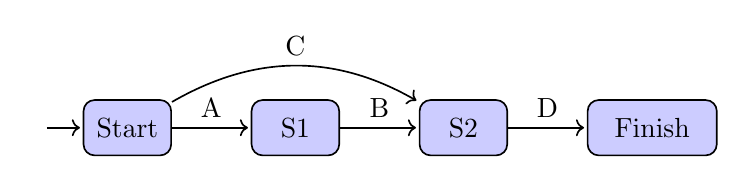
\begin{tikzpicture}[->,shorten >=1pt,auto,column sep=2.2cm,
                    semithick,initial text=]
  \node[initial,block] (s0) {Start};
  \node[block] (s1) [right=of s0] {S1};
  \node[block] (s2) [right=of s1] {S2};
  \node[bw] (s3) [right=of s2] {Finish};

  \path (s0) edge node {A} (s1)
        (s1) edge node {B} (s2)
        (s2) edge node {D} (s3)
        (s0) edge[bend left=30] node {C} (s2);
\end{tikzpicture}
\end{center}

 Having a diagram like this makes it easy to see what can run in parallel and what steps need to happen in what order.  You might not need such a thing, but they are super useful for explaining to nontechnical coworkers or senior management what is happening and how it's going.


\section*{Breaking Dependencies with Speculation}
Let's go back to a real life analogy of speculation. Under normal circumstances, the coffee shop staff waits for you to place your order (``medium double double'') before they start making your order. Sensible. If you go to a certain coffee shop enough, then the staff start to know you and know your typical order and they might speculate about your order and start preparing it in advance, even before you get up to the counter. If they're right, time is saved: your order is ready sooner. If they're wrong, the staff did some unnecessary work and they'll throw away that result and start again with what you did order. If they can predict with high accuracy what you will order, then this is a net savings of time on average.

You can even put some numbers on it! If successfully predicting your order saves 30 seconds per day, and if they're wrong, remaking it takes 3 minutes longer than normal, then if your order is unpredictable one out of every 10 days, how much time is saved? 9 days are correct for a savings of 4.5 minutes, from which we subtract the 3 minute penalty for being wrong, and we've saved 1.5 minutes in the 10 day period (or about 15 seconds per day on average). Not huge, but imagine if the coffee shop can do that for every regular customer. If there are 100 regular customers that's 25 minutes of waiting saved per day! It all adds up.

Mind you, the idea of speculation isn't new in this course.
Recall that computer architects often use speculation to predict branch
targets: the direction of the branch depends on the condition codes
when executing the branch code. To get around having to wait, the processor
speculatively executes one of the branch targets, and cleans up if it
has to.

We can also use speculation at a coarser-grained level and
speculatively parallelize code. We discuss two ways of doing so: one
which we'll call speculative execution, the other value speculation.

\paragraph{Speculative Execution for Threads.} The idea here is to
start up a thread to compute a result that you may or may not need.
Consider the following code:

\begin{lstlisting}[language=Rust]
fn do_work(x: i32, y: i32, threshold: i32) -> i32 {
    let val = long_calculation(x, y);
    if val > threshold {
        return val + second_long_calculation(x, y);
    }
    return val;
}
\end{lstlisting}
Without more information, you don't know whether you'll have to execute
{\tt second\_long\_calculation()} or not; it depends on the return value of
{\tt long\_calculation()}.  Fortunately, the arguments to {\tt second\_long\_calculation()} do not
depend on {\tt long\_calculation()}, so we can call it at any point. 
Here's one way to speculatively thread the work:

\begin{lstlisting}[language=Rust]
fn do_work(x: i32, y: i32, threshold: i32) -> i32 {
    let t1 = thread::spawn(move || {
        return long_calculation(x, y);
    });
    let t2 = thread::spawn(move || {
        return second_long_calculation(x, y);
    });
    let val = t1.join().unwrap();
    let v2 = t2.join().unwrap();
    if val > threshold {
        return val + v2;
    }
    return val;
}
\end{lstlisting}
We now execute both of the calculations in parallel and return the same
result as before. Is this the only way to do it? No. The current thread is a valid thread for doing work and we don't have to create two threads and join two threads: we can create one and maybe have less overhead.

\begin{lstlisting}[language=Rust]
fn do_work(x: i32, y: i32, threshold: i32) -> i32 {
    let t1 = thread::spawn(move || {
        return second_long_calculation(x, y);
    });
    let val = long_calculation(x, y);
    let v2 = t1.join().unwrap();
    if val > threshold {
        return val + v2;
    }
    return val;
}
\end{lstlisting}

{\sf Intuitively: when is this code faster? When is it slower? How
  could you improve the use of threads?}\\[4em]

We can model the above code by estimating the probability $p$ that
the second calculation needs to run, the time $T_1$ that it takes
to run {\tt long\_calculation}, the time $T_2$ that it takes to run
{\tt second\_long\_calculation}, and synchronization overhead $S$.
Then the original code takes time
\[ T = T_1 + p T_2, \]
while the speculative code takes time
\[ T_s = \max(T_1, T_2) + S.\]

\paragraph{Exercise.} Symbolically compute when it's profitable to do the
speculation as shown above. There are two cases: $T_1 > T_2$ and $T_1
< T_2$. (You can ignore $T_1 = T_2$.)


\paragraph{Value Speculation.}
The other kind of speculation is value speculation. In this case,
there is a (true) dependency between the result of a computation 
and its successor:
% note: v1 is meant to be the result you get from longCalculation this time, while last_value is what you got last time. (The code doesn't show that). If you get the same result from longCalculation this time as you did last time, then secondLongCalculation is correct and you don't need to redo it.

\begin{lstlisting}[language=Rust]
fn do_other_work(x: i32, y: i32) -> i32 {
    let val = long_calculation(x, y);
    return second_long_calculation(val);
}
\end{lstlisting}

If the result of {\tt value} is predictable, then we can speculatively
execute {\tt second\_long\_calculation} based on the predicted value.
(Most values in programs are indeed predictable). If 90\% of customers are using the standard billing plan, you might assume that that's correct in your calculations, and then change that later if it turns out you are wrong. Or you might have a software cache where you keep the latest state so you don't have to go to the database to check a value that changes rarely. 

\begin{lstlisting}[language=Rust]
fn do_other_work(x: i32, y: i32, last_value: i32) -> i32 {
    let t = thread::spawn(move || {
        return second_long_calculation(last_value);
    });
    let val = long_calculation(x, y);
    let v2 = t.join().unwrap();
    if val == last_value {
        return v2;
    }
    return second_long_calculation(val);
}
\end{lstlisting}

Note that this is somewhat similar to memoization, except with 
parallelization thrown in. In this case, the original running time is
\[ T = T_1 + T_2, \]
while the speculatively parallelized code takes time
\[ T_s = \max(T_1, T_2) + S + pT_2,\]
where $S$ is still the synchronization overhead, and $p$ is the probability that
\verb+val != last_value+.

\paragraph{Exercise.} Do the same computation as for speculative execution.

\subsection*{When can we speculate?}
Speculation isn't always safe. We need the following conditions:
  \begin{itemize}
    \item {\tt long\_calculation} and {\tt second\_long\_calculation} must not call
      each other.
    \item {\tt second\_long\_calculation} must not depend on
      any values set or modified by {\tt long\_calculation}.
    \item The return value of {\tt long\_calculation} must be deterministic.
  \end{itemize}

As a general warning: Consider the \emph{side effects} of function calls. Oh, let's talk about side effects. Why not. They have a big impact on parallelism. Side effects are problematic, but why? For one thing they're kind of unpredictable (why does calling this function result in unexpected changes elsewhere?!). Side effects are changes in state that do not depend on the function input. Calling a function or expression has a side effect if it has some visible effect on the outside world. Some things necessarily have side effects, like printing to the console. Others are side effects which may be avoidable if we can help it, like modifying a global variable. As we've seen, Rust discourages those kinds of problems but doesn't forbid them: we can still have atomic types shared that would represent some sort of global state.


\section*{Software Transactional Memory}
Somewhat related to the idea of speculation is the idea of software transactional memory. In this case, a group of changes are carried out on a speculative basis, assuming that they will succeed, and we'll check afterwards if everything is okay and retry if necessary~\cite{stm}. 

There is a library for this in Rust\footnote{\url{https://github.com/Marthog/rust-stm}} although we can't vouch for its quality or usefulness. Developers use software transactions by writing {\tt atomic} blocks:
\begin{lstlisting}[language=Rust]
let x = atomically(|trans| {
    var.write(trans, 42)?; // Pass failure to parent.
    var.read(trans) // Return the value saved in var.
});
\end{lstlisting}
The idea resembles database transactions, which most likely you know about
The {\tt atomic} construct means that either the code in
the atomic block executes completely, or aborts/rolls back in the
event of a conflict with another transaction (which triggers a retry
later on, and repeated retries if necessary to get it applied).

\paragraph{Benefit.} The big win from transactional memory is the simple
programming model. It is far easier to program with transactions than with
locks. Just stick everything in an atomic block and hope the compiler does the
right thing with respect to optimizing the code.

\paragraph{Motivating Example.} We'll illustrate STM with the usual bank account example\footnote{It turns out that bank account transactions aren't actually atomic, but they still make a good example.}.
\begin{lstlisting}[language=Rust]
struct Account {
    balance: TVar<f32>,
}

fn transfer_funds(sender: &mut Account, receiver: &mut Account, amount: f32) {
    atomically(|tx| {
        let sender_balance = sender.balance.read(tx)?;
        let receiver_balance = receiver.balance.read(tx)?;
        sender.balance.write(tx, sender_balance - amount)?;
        receiver.balance.write(tx, receiver_balance + amount)?;
        Ok(0)
    });
}
\end{lstlisting}

Using locks, we have two main options:
      \begin{itemize}
        \item Big Global Lock: Lock everything to do with modifying accounts. This is slow and serializes your program.
        \item Use a different lock for every account. Prone to deadlocks; high overhead.
      \end{itemize}
With STM, we do not have to worry about remembering to acquire locks,
or about deadlocks.

\paragraph{Drawbacks.} As I understand it, three of the problems with 
transactions are as follows:

\begin{itemize}
\item I/O: Rollback is key. The problem with transactions and I/O is
  not really possible to rollback. (How do you rollback a write to the
  screen, or to the network?)

\item Nested transactions: The concept of nesting transactions is easy
  to understand. The problem is: what do you do when you commit the
  inner transaction but abort the nested transaction? The clean
  transactional fa\c{c}ade doesn't work anymore in the presence of
  nested transactions. (The Rust library will panic at runtime if you try to nest transactions)

\item Transaction size: Some transaction implementations (like
  all-hardware implementations) have size limits for their
  transactions.
\end{itemize}

\paragraph{Implementations.} Transaction implementations are typically 
optimistic; they assume that the transaction is going to succeed,
buffering the changes that they are carrying out, and rolling back the
changes if necessary.

One way of implementing transactions is by using hardware support,
especially the cache hardware. Briefly, you use the caches to store
changes that haven't yet been committed. Hardware-only transaction
implementations often have maximum-transaction-size limits, which are
bad for programmability, and combining hardware and software approaches
can help avoid that.

\paragraph{Implementation issues.} Since atomic sections don't protect
against data races, but just rollback to recover, a datarace may still
trigger problems in your program.

\begin{tabular}{r|l}
\begin{minipage}{.46\textwidth}
\begin{lstlisting}[language=Rust]
fn what_could_go_wrong(x: TVar<i32>, y: TVar<i32>) {
    atomically(|t| {
        let old_x = x.read(t)?;
        let old_y = y.read(t)?;
        x.write(t, old_x + 1);
        y.write(t, old_y + 1);
        Ok(0)
    });
}
\end{lstlisting}
\end{minipage}
&
\begin{minipage}{.52\textwidth}
\begin{lstlisting}[language=Rust]
fn oh_no(x: TVar<i32>, y: TVar<i32>) {
    atomically(|transaction| {
        if x.read(transaction)? != y.read(transaction)? {
            loop { /* Cursed Thread */}
        }
        Ok(0)
    });
}
\end{lstlisting}
\end{minipage}
\end{tabular}

In this silly example, assume initially {\tt x = y}. You may think the
code will not go into an infinite loop, but it can. That's because intermediate states can still become visible! Although the block is atomic, that just means the changes succeed or are rolled back as a group; it does not mean that another thread cannot read \texttt{x} and \texttt{y} and see them at some partial-completion state of the transaction. (Maybe this doesn't happen in the Rust implementation, but it certainly can in C/\CPP~versions of STM.)










\chapter*{13--- Early Termination, Reduced-Resource Computation}

\addcontentsline{toc}{chapter}{13--- Early Termination, Reduced-Resource Computation}

\section*{Trading Accuracy for Time}

Knowing when to quit is wise. In some cases, we can speed up our program by not waiting for the slowest steps to be done. This is somewhat related to speculation, but the big distinction is that in speculation we do extra work ``just in case'' and with early phase termination, we skip doing some work even though we're supposed to do on the basis of ``close enough is good enough''.  There are two basic ideas: the first way is to skip some parts of work and the second is to intentionally reduce accuracy to speed things up. 

You may implement these strategies when you're writing an exam: time is limited and you might choose not to do a certain question because the benefit is small and you can use your time better doing a different question. In which case you might leave question 3.2 blank in favour of working on question 4.1. That's where you skip some work. Alternatively, you could choose to skip error handling in question 4.1, knowing that you will lose some marks in that question but freeing up some more time to do question 3.2. Exams are nice (or nasty) in that we can do both things, but your program might support only one.

\subsection*{Early Phase Termination}

The formal name for the first idea, quitting early, is is early phase
termination~\cite{Rinard:2007:EarlyPhaseTermination}. So, to apply it to a concrete idea: we've talked about barriers quite a bit. Recall that the idea is that
no thread may proceed past a barrier until all of the threads
reach the barrier. Waiting for other threads causes delays. 
Killing slow threads obviously speeds up the program. Well, that's easy.

\begin{center}
``Oh no, that's going to change the meaning of the program!''
\end{center}

Let's consider some arguments about when it may be acceptable to just
kill (discard) tasks. Since we're not completely crazy, we can develop
a statistical model of the program behaviour, and make sure that the
tasks we kill don't introduce unacceptable distortions. Then when we
run the program, we get an output and a confidence interval.

If you wanted a game-relevant example, pretend you're really bad at Mario Kart. If you're in last place when the second-last player (or AI) drives across the finish line, the race is over at that point because we already know you finished last (``Oh nooo!''). There's no benefit to waiting while you have to drive the rest of the lap to the finish. In that case, ending the race while one driver has not yet finished is perfectly safe because the outcome is already known: I'm really bad at Mario Kart.

\paragraph{Should Have Made A Left Turn At Albuquerque.} 
Many problems are mathematically hard in nature: to find the optimal solution you have to consider every possibility. Well, what this strategy presupposes is: don't. Imagine the travelling salesperson problem, just for the sake of an example. There are $n$ points to visit and you want to minimize the amount of travel time. The only way to know if a solution is best is to consider every possible route.

One way we can know if we're wasting time is to remember previous outcomes. The solution we're evaluating will have some travel cost in units (maybe kms). If the currently-accumulated cost in kms is larger than the total of the thus-far best solution, give up. To be specific, if we have a route that has 400 km of driving and we are partway through building a solution and we have already got 412 km of driving, we can give up on this option (and not evaluate the rest of it) because we already know it won't be the best.

Another approach is to stop as soon as you have a solution that's reasonable. If our target is to get total travel under 500 km then we can stop searching as soon as we find one that satisfies this constraint. Yes, we might stop at 499 km and the optimal solution might be 400 (25\% more driving for the poor peon) -- but it does not have to be perfect; it just has to be acceptable. And if traffic in the hypothetical region is anything like that of the GTA, the route that is shortest in kilometres may not be the shortest in terms of time anyway.

You can also choose to reduce the amount of effort by trying, say, five or ten different possibilities and seeing which of those is the best. There's no guarantee you'll get an optimal solution: you might have randomly chosen the ten worst options you could choose. 

Interesting to think about: what does Google Maps do? For some problems there are relatively few solutions; if you plan to drive in the Yukon territory there are a finite set of roads to travel. But suppose you're driving around Toronto; the grid system means there are lots and lots of options, right? Maybe some heuristic is used to generate some possibilities and the best ones of those are chosen.


\paragraph{This Point is Too Hard.} Monte Carlo simulations
are a good candidate; you're already picking points randomly.
Raytracers can work as well. Both of these examples could spawn a lot
of threads and wait for all threads to complete. For mathematical functions that are ``not nice'', different points might take longer to evaluate than others. 
In either case, you
can compensate for missing data points, assuming that they look similar to
the ones that you did compute. If you have a function where some graph is being
computed, you can probably guess that a missing point is somewhere in between the two (or $n$) nearest points. So just average them.

The same is true for graphics, of course: if rendering a particular pixel did
not go well for some reason, you can just average the adjacent ones and probably
people would not notice the difference. Not bad!

In other cases, some threads simply take too long, but we don't need all of them to produce a result. If we are evaluating some protocol where the majority wins, we can stop as soon as sufficient results have been returned; either an outright majority for an option or that the remaining votes couldn't change the outcome. This happens to some extent with election projections: even if not all polling stations are reporting a result, news channels will declare a winner if the remaining votes would not be enough to change the outcome. Actually, news channels probably take it a bit too far in that they will declare a winner even if the outstanding votes exceed the margin, on a theory that it probably won't be the case that they are 100\% for the candidate who is in second place. But they can be wrong.

\paragraph{Slow Road...}
For some categories of problem, we know not only that a solution will exist, but also how many steps it takes to solve (optimally). Consider the Rubik's Cube -- it's much easier to explain if you have seen one. It'll appear in the slides, but if you're just reading the note(book/s) then I suggest you google it\footnote{If you've waited for the exam to read this and you can't google... whoops!}.

This is a problem with a huge number of possible permutations and brute force isn't going to work. However, research has proven that no matter what the state of the cube is, it can be transitioned to a solved state in 20 moves or fewer. This number is called God's Number, presumably because it is the maximum number of moves it would take an all-knowing deity to solve the puzzle. So if you have a solver for a Rubik's cube, and if you don't find a solution in (fewer than) 20 moves, you should cancel this solution attempt and try another one.

Okay, that's fun to talk about, but it's always better if we see it in action? Let's play around with \url{https://rubiks-cube-solver.com/}, which implements this very behaviour. It says in their description of how it works that it runs an open source algorithm; it looks for a solution in 20 steps or fewer. This implementation does both kinds of tradeoff: if the solution being evaluated takes too long it's killed. And if no under-20-move solution has been found within a certain time limit, it will return a solution that takes 24 steps and give you a less optimal solution. That's actually an example of reducing accuracy (quality of solution) for speed, which leads us into our next approach.

\subsection*{Reduced-Resource Computation}

The formal name for the second idea is ``reduced resource computation'' -- that is to say, we do more with less! Austerity programs for our computer programs. Well, you can use \texttt{float} instead of \texttt{double}. But you can also work with integers to represent floating point numbers (e.g., representing money in an integer number of cents). But let's really  think about when this is appropriate.

\paragraph{Circuit... Analysis!} Recall that, in scientific computations, you're entering points that were measured (with some error) and that you're computing using machine numbers (also with some error). Computers are only providing simulations, not the ground truth; the question is whether the simulation is good enough.

Imagine that the simulation is deciding on what resistors are going to be put in your circuit board: is there any point in calculating it down to five decimal places when the resistors you buy have a tolerance of $\pm$5\%? No, and if you took a circuits course with Prof. Barby he would be very disappointed if you said yes.


\paragraph{iddqd.} Perhaps my favourite example of trading accuracy for time is a function in Quake III, contributed by John Carmack known as ``fast inverse square root''. For graphics processing, sometimes you want to calculate $1/\sqrt{x}$. This is important because you use it in calculating lighting and reflections (because you normalize vectors). Normalizing is mostly a straightforward exercise: square some numbers, add them up, and then... oh no, you have to use square root... That one isn't so simple.

Square root (or similar) is usually calculated by some interpolation or root-finding method (if you took a numerical methods course, you know several techniques for calculating this). But instead there's this~\cite{fisqrt}. 

\begin{lstlisting}[language=C]
float FastInvSqrt(float x) {
  float xhalf = 0.5f * x;
  int i = *(int*)&x;         // evil floating point bit level hacking
  i = 0x5f3759df - (i >> 1);  // what the fuck?
  x = *(float*)&i;
  x = x*(1.5f-(xhalf*x*x));
  return x;
}
\end{lstlisting}

The first line of the function is straightforward - take half the value of \texttt{x}. The second one says to interpret the value of \texttt{x} as an \texttt{int}. Now this probably seems like dark magic, and it is. Pretend this floating point number is an integer. I mean, you can, but why does this make sense? 

There's a lot of explanation and a lot of math in the source material but it comes down to how the float is stored. The float starts with a sign bit, then the exponent, and then the mantissa (math reminder: in $1.95 \times 10^{3}$, the exponent is 3 and the mantissa is 1.95).

The clever hack is somewhat obsoleted now by the fact that CPU instructions now exist to give you fast inverse square root. This was obviously not something you could rely on in 1999, but we're going to revisit the idea of using clever CPU instructions to speed things along in the next lecture. So if we say pretend this float is an integer we end up with this~\cite{fisqrt2}:

\begin{center}
	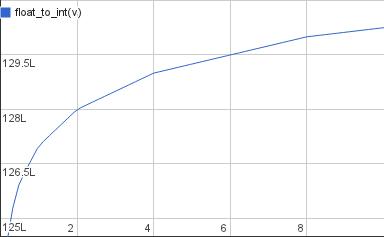
\includegraphics[width=0.4\textwidth]{images/float-to-int.png}
\end{center}

If it's not obvious, this plot rather resembles the plot of $-1/\sqrt{x}$. So we are pretty close to getting where we need to go. All we need is to invert it and then do a little bit of an offset. The seemingly magic number of \texttt{0x5f3759df} is not a bit pattern, but just a calculated offset to make the approximation a little bit better. Then we turn it back into a float.

The last step is then to do one quick iteration of Newton's method to refine the calculation a little bit and we have a great solution: it is a fast, constant-time calculation for something that normally would be difficult, and it's very accurate, something like 0.175\% error at the most. And in a 3D game a tiny inaccuracy is not a big deal! Especially in one from 1999. It wasn't exactly photorealistic to begin with, now was it...?

This is the best case scenario: the accuracy that we trade for speed is both very small and its application is one in which a small difference is not noticeable. This is beyond ``close enough is good enough'', this is hardly any tradeoff at all.


\paragraph{N-Body Problem}
A common physics problem that programmers are asked to simulate is the N-Body problem: you have some number of bodies (N, obviously) and they interact via gravitational forces. The program needs to compute the movements of the bodies over time. This is a typical example of a program that is well suited to parallelization: you can compute the forces on each body $n$ from all other bodies in parallel. This was even at one time an OpenCL assignment in this course, although now there are too many good solutions on the internet so it was replaced. Bummer.

What can you do here if you want to speed it up even more? You could look for optimizations that trade off accuracy for performance. As you might imagine, using \texttt{float} instead of \texttt{double} can save half the space which should make things quite a bit faster. But you want more...

Then we need some domain knowledge. That is, we need to think about what we know about the problem and we can make a decision about what is important and what is not. If we thought about what's important for determining the forces, what would we consider to be the most important? 

Hint: consider the formula: $F = \dfrac{Gm_{1}m_{2}}{r^{2}}$. 

Force is a function of how close the objects are. Thus, points that are far away contribute only small forces. So you can estimate them (crudely). A first approximation might say that forces that are far enough away are zero. In principle, Jupiter has a gravitational influence on the rate of descent if I drop a whiteboard marker (whether positive, negative, or zero depends on its relative position at the time of my clumsiness), but the effect is so incredibly small as to be worth ignoring. But what about objects that are not exactly close by, but also not so far away as to be irrelevant?

The idea is to divide the points into a number of ``bins'' which are cubes representing a locale of some sort. Then, compute the centre of mass for each bin. When calculating the forces on a given point, add the force exerted by the centre of mass for faraway bins to the force exerted by individual particles for nearby particles.

A more concrete explanation with an example: suppose the space  is divided into $[0, 1000]^3$, so we can take bins which are cubes of length 100. This gives 1000 bins. If you want to increase the accuracy, increase the number of bins. If you want to increase the speed, decrease the number of bins: either make bins larger, or change your definition of what is too far away to care about.

The program should have a 3-dimensional array {\tt cm} of a point structure to store centres-of-mass. The {\tt x}, {\tt y} and {\tt z}
components contain the average position of the centres of mass of a
bin, while the {\tt mass} component stores the total mass. Compute all of
the masses in parallel: create one thread per bin, and add a point's
position if it belongs to the bin, e.g.

\begin{lstlisting}[language=Rust]
struct Point {
    x: f32,
    y: f32,
    z: f32,
    mass: f32,
}
\end{lstlisting}

Let's start there. We are going to improve this by adding a \texttt{bin} property to each point, so that we know what bin it is in. Later, we can use the bin to know if another point is considered close by. In my example, I calculate the bin at the same time as the point is randomly generated, because why iterate over the collection a second time?

Once all points are generated, we can calculate the centre of mass for each bin. This is, of course, just a weighted average of all the points in that bin and is straightforward to calculate.

The payoff from all these calculations is to save time while
calculating forces. In this example, we'll compute exact
forces for the points in the same bin and the directly-adjacent bins
in each direction (think of a Rubik's Cube; that makes 27 bins in all,
with 6 bins sharing a square, 12 bins sharing an edge, and 8 bins
sharing a vertex with the centre bin). If there is no adjacent bin 
(i.e., this is an edge), just act as if there are no points 
in the place where the nonexistent bin would be. 

This does mean there is overhead for each step, meaning the total amount of overhead goes up. We had to (1) calculate what bin this is, (2) calculate the centre of mass for each bin, and (3) decide when we should use the centre-of-mass calculation or the exact calculation.

Here's some data calculated with 100~000 points (using \texttt{hyperfine -m 5 "cargo run --release"}). The unmodified version takes about 162 seconds; the modified version takes about 147. With smaller numbers of points, the difference is not as noticeable, but still consistent. With 50~000 the original \texttt{nbody} program takes about 39 seconds on average and the optimized about 37, so a slight speedup! The amount of benefit increases with more points, but doesn't keep up with the computational complexity of the increase in the number of points.

Also, this is before any parallelization (no threads are spawned). We can calculate forces on each point pretty effectively in parallel; we can also parallelize the calculations of the centre of mass quite easily. Both would speed up the program quite a lot! 

If I just parallelize version without approximations (using the rayon parallel iterator), it takes about 25 seconds to run, and parallelizing the version with bins (using the same in a very naive parallelization) gets the execution time for 100~000 points down to about the same 25 seconds. It is clear that parallelizing the problem has a much greater effect than the tradeoff of accuracy for time (at least in this implementation), but on a sufficiently large problem, everything counts.


\subsection*{Loop perforation} 
You can also apply the same idea to sequential programs. Instead
of discarding tasks, the idea here is to discard loop iterations~\cite{hoffmann09:_using_code_perfor_improv_perfor}.
Here's a simple example: instead of the loop,
\begin{center}
\verb|for i in 0 .. n { sum += numbers.get(i).unwrap(); }|
\end{center} \vspace*{-1em}
simply write,
\vspace*{-1em}\begin{center}
\verb|for i in (0 .. n).step_by(2) { sum += numbers.get(i).unwrap(); }|
\end{center}
and multiply the end result by a factor of 2. This only works 
if the inputs are appropriately distributed, but it does give a
factor 2 speedup.

\paragraph{Example domains.} In~\cite{Rinard:2010:PSA:1932682.1869525},
we can read that loop perforation works for evaluating forces on water
molecules (in particular, summing numbers); Monte-Carlo simulation for
swaption pricing; and video encoding. In that example, changing loop
increments from 4 to 8 gives a speedup of 1.67, a signal to noise ratio
decrease of $0.87\%$, and a bitrate increase of $18.47\%$, producing
visually indistinguishable results. 










\chapter*{14 --- Memory Consistency}

\addcontentsline{toc}{chapter}{14 --- Memory Consistency}

\section*{Memory Consistency, Memory Barriers, and Reordering}
Previously, when atomics were introduced, we said to use sequential consistency without much detail and without discussing the other options. Now it's time to learn about it. We'll cover both instruction reordering by
the CPU and reordering initiated by the compiler.  

\paragraph{Compiler Reordering.} When asked to compile code, the compiler does not take every statement that you provide and translate it into a (set of) machine language instruction(s). The compiler can change the order of certain events. The compiler will be aware of things like load-delay slots and can swap the order of instructions to make use of those slots more effectively. In the (silly) example on the left there might be a stall while we wait for \texttt{x} to be available before we can send it in to the \texttt{println!} macro; on the right we moved two unrelated instructions into the delay slots. So that feels like free performance! 

\begin{multicols}{2}
\begin{lstlisting}[language=Rust]
let x = thing.y;
println!("x = {}", x);
z = z + 1;
a = b + c;
\end{lstlisting}
\columnbreak
\begin{lstlisting}[language=Rust]
let x = thing.y;
z = z + 1;
a = b + c;
println!("x = {}", x);
\end{lstlisting}
\end{multicols}

We'll talk about other compiler optimizations soon, but we don't want to get away from the topic of reordering. 

\paragraph{Hardware Reordering.} In addition to the compiler reordering, the hardware can do some reordering of its own. A sequence of instructions is provided to the CPU, and it can decide it would rather do them in an order it finds more convenient. That is fairly straightforward.

There is another possibility we have to consider, and it is updates from other threads. When a thread is doing a check on a variable, such as a quit condition (exit the loop if \texttt{quit} is now true), how do we know if we have the most up-to-date value for \texttt{quit}? We know from the discussion of cache coherence that the cache will be updated via snooping, but we need a bit more reassurance that the value we're seeing is the latest one. How could we get the wrong order? If the read by thread $A$ is reordered by the hardware so that it's after the write by thread $B$, then we'll see the ``wrong'' answer. 

Different hardware provides different guarantees about what reorderings it won't do. Old 386 CPUs didn't do any; x86 usually won't (except where there are some specific violations of that; but ARM has weak ordering except where there are data dependencies~\cite{weakvsstrong}. ARM is getting pretty popular, so we do have to care about hardware reorderings, unfortunately.

\paragraph{I have a plan, but it's a bad one.}

There are some reorderings where we are easily able to conclude that it is okay and safe to do, but not every reordering is. In an obvious case, if the lines of code are \texttt{ z *= 2 } and \texttt {z += 1} then neither the compiler nor hardware will reorder those because it knows that it would change the outcome and produce the wrong answer. There's a clear data dependency there, so the reordering won't happen. There are a couple of hardware architectures where that isn't respected, but we'll ignore them for now.

But what if there's no such clear dependency? Consider something like this pseudocode:

\begin{multicols}{2}
\begin{verbatim}
lock mutex for point
point.x = 42;
point.y = -42;
point.z = 0;
unlock mutex for point
\end{verbatim}
\columnbreak
\begin{verbatim}
lock mutex for point
point.x = 42;
point.y = -42;
unlock mutex for point
point.z = 0;
\end{verbatim}
\end{multicols}

Wait a minute --- that's not an okay reordering, because now an element of the point is being accessed outside of the critical section and we don't want that. It's a reordering, alright, in that the store of \texttt{point.z} has been moved to after the store of state of the mutex (unlock does, after all, change its state). What we need is a way to tell the compiler (and hardware) that this is not okay.


\paragraph{Sequential Consistency.} In a sequential program, you expect
things to happen in the order that you wrote them. So, consider this code,
where variables are initialized to 0:

\begin{center}
\begin{lstlisting}
    T1: x = 1; r1 = y;
    T2: y = 1; r2 = x;
\end{lstlisting}
\end{center}
We would expect that we would always query the memory and get a state
where some subset of these partially-ordered statements would have executed.
This is the \emph{sequentially consistent} memory model. A simple description: (1) each thread induces an \emph{execution trace}; and (2) always, the program has executed some prefix of each thread's trace. Or, alternatively:

\begin{quote}
``... the result of any execution is the same as if the operations of all the processors were executed in some sequential order, and the operations of each individual processor appear in this sequence in the order specified by its program.'' --- Leslie Lamport
\end{quote}


It turns out that sequential consistency is expensive to implement.
Think how much coordination is needed to get a few people to agree on where to go for lunch; now try to get a group of people to agree on what order things happened in. Right. Now imagine it's a disagreement between threads so they don't have the ability to negotiate. So most systems actually implement weaker memory models, such that both {\tt r1} and {\tt r2} might end up unchanged.

Allowing some reorderings could potentially significantly speed up the program! If left to its own devices, the compiler could reorder anything, but we need to tell it what is allowed and what is disallowed. 

\subsection*{Memory Consistency Models}

Rust uses the same memory consistency models as \CPP. The Rustonomicon (book of names of Rust\footnote{Not to be confused with the Necronomicon...}) says pretty directly that this is not because the model is easy to understand, but because it's the best attempt we have at modelling atomics because it is a very difficult subject. The idea behind the memory model is to have a good way of talking about the \textit{causality} of the program. While causality definitely sounds like something Commander La Forge would talk about on the \textit{Enterprise}, in this case it means establishing relationships between events such as ``event A happens before event B''. 

You will recall from the introduction to the subject of concurrency that we frequently sought the same thing in our program at a higher level, when we'd say that we can use a semaphore to ensure that one thing happens before another. The idea is the same, but our toolkit is a little bit different: it's the \emph{memory barrier} or
\emph{fence}. 

This type of barrier prevents reordering, or,
equivalently, ensures that memory operations become visible in the
right order. A memory barrier ensures that no access occurring after
the barrier becomes visible to the system, or takes effect, until
after all accesses before the barrier become visible.


The x86 architecture defines the following types of memory 
barriers:

\begin{itemize}
\item {\tt mfence.} All loads and stores before the barrier become
visible before any loads and stores after the barrier become visible.
\item {\tt sfence.} All stores before the barrier become visible before
all stores after the barrier become visible.
\item {\tt lfence.} All loads before the barrier become visible before
all loads after the barrier become visible.
\end{itemize}

Note, however, that while an {\tt sfence} makes the stores visible,
another CPU will have to execute an {\tt lfence} or {\tt mfence} to
read the stores in the right order.

Consider the example again:
  \begin{lstlisting}[language=C]
                         f = 0

/* thread 1 */                     /* thread 2 */
while (f == 0) /* spin */;         x = 42;
// memory fence                    // memory fence
printf("%d", x);                   f = 1;
  \end{lstlisting}
This now prevents reordering, and we get the expected result.

Memory fences are costly in performance. It makes sense when we think about it, since it (1) prevents re-orderings that would otherwise speed up the program; and (2) can force a thread to wait for another one. Sequential consistency will necessarily result in memory fences being generated to produce the correct results. 

\subsection*{Other Orderings}
The \CPP~standard includes a few other orderings that don't appear in this section because they aren't in Rust. But we'll cover Acquire-Release and Relaxed briefly. Neither comes with a recommendation to use it, but if you can prove that your use of it is correct, then you can do it. It may give a slight performance edge.

Acquire means that accesses (reads or writes) after the acquire operation can't move to be before the acquire. Release means accesses before the release operation can't move to be after the release. They make a good team: by placing acquire at the start of a section and release after, anything in there is ``trapped'' and can't get out.

That makes them the perfect combination for a critical section: acquire prevents things from moving from inside the critical section to before the critical section; release prevents things from inside from moving to after the critical section. Nice! 

Here's an example of acquire and release, as taken from the Rustonomicon's page about atomics ( \url{https://doc.rust-lang.org/nomicon/atomics.html}. It's implementing a spinlock: 

\begin{lstlisting}[language=Rust]
use std::sync::Arc;
use std::sync::atomic::{AtomicBool, Ordering};
use std::thread;

fn main() {
    let lock = Arc::new(AtomicBool::new(false)); // value answers "am I locked?"

    // ... distribute lock to threads somehow ...

    // Try to acquire the lock by setting it to true
    while lock.compare_and_swap(false, true, Ordering::Acquire) { }
    // broke out of the loop, so we successfully acquired the lock!

    // ... scary data accesses ...

    // ok we're done, release the lock
    lock.store(false, Ordering::Release);
}
\end{lstlisting}

The acquire and release semantics keep all the things that should be in the critical section inside it.

And then there is relaxed. Relaxed really does mean the compiler will take it easy, and all reorderings are possible. Even ones that you might not want! The Rustonomicon suggests one possible valid use for that scenario is a counter that simply adds and you aren't using the counter to synchronize any action. Something like atomically counting the requests to each resource might be suitable. You can report the counters as metrics and it's not super important that request 9591's increment of the counter occurs before that of request 9598. It's all the same in the end...

\subsection*{Matters, Order Does}
There have been a few reminders to use sequential consistency because atomics are hard to reason about and it's easy to get it wrong. But does this happen in reality? Yes, and here's an example of it in Rust~\cite{weakbug}.

The observed behaviour was an inconsistent state being reported by an assertion; when looking at the registers the registers contained garbage even though it was just after a read that should have loaded it in. That's hard to notice and difficult to debug as well, because running in debug mode might prevent the reordering in the first place.

You can actually look at the fix applied to the lock-free queue at \url{https://github.com/crossbeam-rs/crossbeam/pull/98/files}. But the short summary is that the load of the \texttt{ready} property needs to have at least Acquire semantics and the store of it should have release.  If we don't do that, we might attempt to park the thread early. 









\chapter*{15 --- Crossbeam and Rayon}

\addcontentsline{toc}{chapter}{15 --- Crossbeam and Rayon}

\section*{Use Libs Wisely!}
In previous courses, such as a concurrency course, there was a lot of expectation to do most things the hard way: write your own implementation and don't use libraries. In this course, such restrictions don't apply. In industry, you'll use libraries that have appropriate functionality, assuming the license for them is acceptable to your project. The two we'll talk about today, Crossbeam and Rayon are, for the record, Apache licensed, so it should pose no issue. In the previous version of the course where we used C and \CPP, we taught the OpenMP functionality, which is used to direct the compiler to parallelize things in a pretty concise way. The same idea applies here, except it's using the Crossbeam and Rayon crates rather than compiler directives.


\subsection*{Concurrency with Crossbeam} 

You'll recall from earlier when we introduced threads, that this doesn't work:
\begin{lstlisting}[language=Rust]
use std::thread;

fn main() {
    let v = vec![1, 2, 3];

    let handle = thread::spawn(|| {
        println!("Here's a vector: {:?}", v);
    });

    handle.join().unwrap();
}
\end{lstlisting}

The problem was that the compiler can't tell for sure how long the data is going to live, and we said that we can get around this by moving the vector into the thread and returning it if needed again. Then later, when we wanted to share a Mutex between threads, we used the \texttt{Arc} type. We could have used the \texttt{Arc} type here too, but that's a bit of a pain if the thread is going to be short-lived. Crossbeam gives us the ability to create ``scoped'' threads. Scope is like a little container we are going to put our threads in. It allows the compiler to be convinced that a thread will be joined before leaving the scope (container). Alright, how about this?

\begin{lstlisting}[language=Rust]
fn main() {
    let v = vec![1, 2, 3];

    crossbeam::scope(|scope| {
        println!("Here's a vector: {:?}", v);
    }).unwrap();

    println!("Vector v is back: {:?}", v);
}
\end{lstlisting}

Wait a minute. That's not quite right, because if I add statements where we print the thread ID, I get this output:

{\scriptsize 
\begin{verbatim}
main thread has id 4583173568
Here's a vector: [1, 2, 3]
Now in thread with id 4583173568
Vector v is back: [1, 2, 3]
\end{verbatim}
}

All we did was make the container, but we didn't spawn any threads. Here's a better version:
\begin{lstlisting}[language=Rust]
fn main() {
    let v = vec![1, 2, 3];
    println!("main thread has id {}", thread_id::get());

    crossbeam::scope(|scope| {
        scope.spawn(|inner_scope| {
            println!("Here's a vector: {:?}", v);
            println!("Now in thread with id {}", thread_id::get());
        });
    }).unwrap();

    println!("Vector v is back: {:?}", v);
}
\end{lstlisting}
With output:

{\scriptsize 
\begin{verbatim}
main thread has id 4439997888
Here's a vector: [1, 2, 3]
Now in thread with id 123145430474752
Vector v is back: [1, 2, 3]
\end{verbatim}
}

There are still rules, of course, and you cannot borrow the vector mutably into two threads in the same scope. This does, however, reduce the amount of ceremony required for passing the data back and forth. Wrapping everything in \texttt{Arc} is tedious, to be sure. 


\paragraph{Producer-Consumer with channels.} One of the guidelines that Rust gives is that it's preferable to do message passing as compared to shared memory. Unfortunately, for something like the producer-consumer scenario, the standard multiple-producer-single-consumer channel we are provided won't do; we need a multiple-producer-multiple-consumer channel. And sure enough, Crossbeam gives us one. 

Recall the multi-producer multi-consumer example from earlier. We had to define a shared buffer structure and use semaphores and a mutex to coordinate access, and we saw it's possible to get it wrong in when we drop the mutex. Here's the excerpts from the Crossbeam version. First, a little setup to create a bounded channel with capacity the same as the bounded buffer (100): 

\begin{lstlisting}[language=Rust]
let (send_end, receive_end) = bounded(CHANNEL_CAPACITY);
let send_end = Arc::new(send_end);
let receive_end = Arc::new(receive_end);
\end{lstlisting}

This uses the bounded channel, which has a maximum capacity as specified. If it's full, the sender is blocked until space becomes available. You can also choose an unbounded channel, which allows an arbitrary number at a time (but of course, they have to go somewhere so uncollected messages still take up space in memory and memory is not infinite, but close...).
And look how much simpler the consumer is:
\begin{lstlisting}[language=Rust]
    for _j in 0 .. NUM_THREADS {
        // create consumers
        let receive_end = receive_end.clone();
        threads.push(
            thread::spawn(move || {
                for _k in 0 .. ITEMS_PER_THREAD {
                    let to_consume = receive_end.recv().unwrap();
                    consume_item(to_consume);
                }
            })
        );
    }
\end{lstlisting}

Certainly that's a lot simpler and cleaner, but is it faster? Testing says yes! Hyperfine says the original producer-consumer-opt version takes 372 ms to run for 10000 items consumed per thread, and the version with the channel takes 232. 

\paragraph{Try Again Later.}
Another small thing that Crossbeam enables is an exponential backoff. When attempting to access some resource, we acknowledge that it might not be available right now. If that's the case, an error is not necessarily fatal and the client might want to retry. However, it's very unhelpful to have a tight loop that simply retries as fast as possible. What you should do instead is an exponential backoff: wait a little bit and try again, and if the error occurs, next time wait a little longer.

The idea is that if the resource is not available, repeatedly retrying doesn't help. If it's down for maintenance, it could be quite a while before it's back and calling the endpoint 5 or 10 times every second doesn't make it come back faster and just wastes effort. Or, if the resource is overloaded right now, the reaction of requesting it more will make it even more overloaded and makes the problem worse! And the more failures have occurred, the longer the wait, which gives the service a chance to recover.

Eventually, though, you may have to conclude that there's no point in further retries. At that point you can block the thread or return an error, but setting a cap on the maximum retry attempts is reasonable.

The \texttt{Backoff} util from Crossbeam gives you this functionality. Each step of the backoff takes about double the amount of time of the previous, up to a certain maximum.

Here's an example from the Crossbeam docs of using the backoff in a lock-free loop. Here, the \texttt{spin()} function is used because we can try again immediately. We can do so because if the compare-and-swap operation failed, it's because another did the compare-and-swap and got a chance to run.
\begin{lstlisting}[language=Rust]
use crossbeam_utils::Backoff;
use std::sync::atomic::AtomicUsize;
use std::sync::atomic::Ordering::SeqCst;

fn fetch_mul(a: &AtomicUsize, b: usize) -> usize {
    let backoff = Backoff::new();
    loop {
        let val = a.load(SeqCst);
        if a.compare_and_swap(val, val.wrapping_mul(b), SeqCst) == val {
            return val;
        }
        backoff.spin();
    }
}
\end{lstlisting}

If what we actually need is to wait for another thread to take its turn before we go, we don't want to spin, we want to ``snooze''. This means we'll be waiting longer for the thread to awaken.

\begin{lstlisting}[language=Rust]
fn spin_wait(ready: &AtomicBool) {
    let backoff = Backoff::new();
    while !ready.load(SeqCst) {
        backoff.snooze();
    }
}
\end{lstlisting}

In both cases, the \texttt{backoff} type has a function \texttt{is\_completed} which returns true if the maximum backoff time has been reached and it's advised to give up. And an existing \texttt{backoff} can be re-used if it's reset with the unsurprisingly-named \texttt{reset} function.

Having read a little bit of the source code of the Crossbeam backoff, I'm not sure they implement a little randomness (called jitter). This is an improvement on the algorithm that prevents all threads or callers from retrying at the exact same time. Let me explain with an example: I once wrote a little program that tried synchronizing its threads via the database and had an exponential backoff if the thread in question did not successfully lock the item it wanted. I got a lot of warnings in the log about failing to lock, until I added a little randomness to the delay. It makes sense; if two threads fail at time $X$ and they will both retry at time $X+5$ then they will just fight over the same row. If one thread retries at $X+9$ and another $X+7$, they won't conflict.

The exponential backoff with jitter strategy is good for a scenario where you have lots of independent clients accessing the same resource. If you have one client accessing the resource lots of times, you might want something else; something resembling TCP congestion control. See~\cite{expbackoff} for details. 

\subsection*{Data Parallelism with Rayon}

Looking back at the nbody-bins-parallel code that we discussed earlier, you may have noticed that it contains some includes of a library called Rayon. It's a data parallelism library that's intended to make your sequential computation into a parallel one. In an ideal world, perhaps you've designed your application from the ground up to be easily parallelizable, or use multiple threads from the beginning. That might not be the situation you encounter in practice; you may instead be faced with a program that starts out as serial and you want to parallelize some sections that are slow (or lend themselves well to being done in parallel, at least) without a full or major rewrite.

That's what I wanted to do with the nbody problem. I was able to identify the critical loop (it is, unsurprisingly, in \texttt{calculate\_forces}). We have a vector of points, and if there are $N$ points we can calculate the force on each one independently. 

My initial approach looked at spawning threads and moving stuff into the thread. This eventually ran up against the problem of trying to borrow the \texttt{accelerations} vector as mutable more than once. I have all these points in a collection and I'm never operating on one of them from more than one thread, but a compile time analysis of the borrowing semantics is that the vector is going to more than one thread. The compiler can't prove to itself that my slices will never overlap so they can't all be mutable.

 This is a super common operation, and I know the operation I want to do is correct and won't have race conditions because each element in the vector is being modified only by the one thread. I eventually learned that you can split slices but it was going to be a slightly painful process. You can use \texttt{split\_at\_mut()} and it divides the slice into two pieces... it's a start, but would require doing this multiple times and probably use recursion or similar. Further research eventually told me to stop reinventing the wheel and use a library for this. Thus, Rayon.

\paragraph{Parallelizing loops.} Back on track. A quick glance over this program tells us it is likely that the slow step is computing the interactions. It's reasonably common that computationally-intensive parts of the program happen in a loop, so parallelizing loops is likely to be quite profitable in terms of speeding things up. This is something that Rayon specializes in: it's easy to apply some parallelization directives to the loop to get a large speedup at a small cost (here, cost is programmer time in writing the change and reviewing it).

The line in question where we apply the Rayon library is:
\begin{lstlisting}[language=Rust]
accelerations.par_iter_mut().enumerate().for_each(|(i, current_accel)| {
\end{lstlisting}

A lot happens in this one line, so we need to take a look at it. Normally, we iterate over a collection (here, the accelerations) using an iterator (and it's preferable to the \texttt{for} construction). That's normally a sequential iterator, and the convenient thing about Rayon is that we can drop it in pretty easily. We need to include the ``prelude''. The prelude brings into scope a bunch of traits that are needed for the parallel iterators. Then instead of iterating over the collection sequentially, we use a parallel iterator that produces mutable reference. We effectively ask to have the slices cut up into slices of size 1. I also ask for the enumerate option because I'm going to use the index \texttt{i}, and then I provide the operation that I want to perform: a for-each (where I specify the index name and the name of the variable I want to use for each element in the collection. 

\paragraph{Doing the work.} The description we just saw of dividing up the work is how work units are specified, but doesn't cover what actually happens on execution. After all, if we just divide up the work without having more workers to do it, we're not getting anywhere.

The Rayon FAQ fills in some details about how work gets done. By default, the same number of threads are spawned as available (logical) CPUs (that means hypthereading cores count). These are your workers and the work is balanced using a work-stealing technique. If threads run out of work to do, they steal work from other queues. The technique is based off some foundational work in the area, called Cilk (see~\cite{cilk} for details). 

\paragraph{Maybe too easy?}
We discussed already the effectiveness of this change. And here's how easy it was:

{\scriptsize 
\begin{verbatim}
diff live-coding/L14/nbody-bins/src/main.rs live-coding/L14/nbody-bins-parallel/src/main.rs
2a3
> use rayon::prelude::*;
64c65
<     for i in 0..NUM_POINTS {
---
>     accelerations.par_iter_mut().enumerate().for_each(|(i, current_accel)| {
66d66
<         let current_accel: &mut Acceleration = accelerations.get_mut(i).unwrap();
79,80c79
<     }
< 
---
>     });
\end{verbatim}
}

Why does the ease of doing this matter? Every change we introduce has the possibility of introducing a nonzero number of bugs. If I were to rewrite a lot of code, there would be more opportunities for bugs to appear. This change is minimal and easier for a reviewer to verify that it's correct than a big rearchitecting. And it's faster in terms of dev time -- I can easily drop this in here and then move on to optimizing the next thing. Bugs slow you down.

It is important to note that the iterators do things in parallel, meaning the behaviour of the program can change a bit. If you are printing to the console or writing to a file or something, they can happen out of order when the loop is parallelized, just as they would if you wrote it so that different threads execute.

By that same token, the automatic parallelization doesn't mean there can be no race conditions; thus you still have to satisfy the compiler that your code is correct. If you are trying to find the largest item in an array, we still have to use atomic types or a mutex or similar to ensure that the correct answer is returned. See a quick example below:

\begin{lstlisting}[language=Rust]
use rayon::prelude::*;
use rand::Rng;
use std::i64::MIN;
use std::i64::MAX;
use std::sync::atomic::{AtomicI64, Ordering};

const VEC_SIZE: usize = 10000000;

fn main() {
    let vec = init_vector();
    let max = AtomicI64::new(MIN);
    vec.par_iter().for_each(|n| {
        loop {
            let old = max.load(Ordering::SeqCst);
            if *n <= old {
                break;
            }
            let returned = max.compare_and_swap(old, *n, Ordering::SeqCst);
            if returned == old {
                println!("Swapped {} for {}.", n, old);
                break;
            }
        }
    });
    println!("Max value in the array is {}", max.load(Ordering::SeqCst));
    if max.load(Ordering::SeqCst) == MAX {
        println!("This is the max value for an i64.")
    }
}

fn init_vector() -> Vec<i64> {
    let mut rng = rand::thread_rng();
    let mut vec = Vec::new();
    for _i in 0 ..VEC_SIZE {
        vec.push(rng.gen::<i64>())
    }
    vec
}
\end{lstlisting}

Here, the vector is iterated over in parallel and it's not using the mutable parallel iterator. This code example uses an atomic type, but if I change this to use a \texttt{Mutex} instead of an atomic type (see code below) it increases the runtime from about 121.6~ms to about 871.7~ms (tested with hyperfine as per usual).

\begin{lstlisting}[language=Rust]
fn main() {
    let vec = init_vector();
    let max = Mutex::new(MIN);
    vec.par_iter().for_each(|n| {
        let mut m = max.lock().unwrap();
        if *n > *m {
            *m = *n;
        }
    });
    let m = max.lock().unwrap();
    println!("Max value in the array is {}", m);
    if *m == MAX {
        println!("This is the max value for an i64.")
    }
}
\end{lstlisting}

 The non-parallel code takes about 136.2~ms. This problem doesn't have enough work to parallelize effectively. While the lock-free version speeds it up a small amount, the mutex version was easier to write (and is therefore what you would probably do) but made it much slower. So it's important to consider carefully when to apply the library, because a speedup is not guaranteed just by parallelizing a given loop.









\chapter*{16 --- Mostly Data Parallelism}

\addcontentsline{toc}{chapter}{16 --- Mostly Data Parallelism}


\section*{Data and Task Parallelism}
There are two broad categories of paralellism: data parallelism and
task parallelism. An analogy to data parallelism is hiring a call
center to (incompetently) handle large volumes of support calls,
\emph{all in the same way}. Assembly lines are an analogy to task
parallelism: each worker does a \emph{different} thing.

More precisely, in data parallelism, multiple threads perform the
\emph{same} operation on separate data items. For instance, you have a
big array and want to double all of the elements. Assign part of the
array to each thread. Each thread does the same thing: double array
elements.

In task parallelism, multiple threads perform \emph{different}
operations on separate data items. So you might have a thread that
renders frames and a thread that compresses frames and combines them
into a single movie file.

%We'll continue by looking at a number of parallelization patterns,
%examples of how to apply them, and situations where they might apply.

\subsection*{You're not using those bytes, are you?}
So as a first idea we might think of saving some space by considering the range of, for example, an integer. An \texttt{i32} is 4 bytes. (In C, \texttt{int} is usually 4, though only guaranteed to be at least 2). If we have an integer array of capacity $N$ that uses $N \times 4$ bytes and if we want to do something like increment each element, we iterate over the array and increment it, which is a read of 4 and write of 4. Now, if we could live with limiting our maximum value from 2,147,483,647 (signed, or 4,294,967,295 unsigned) to 32,767  (signed, or 65,535 unsigned), we could reduce in half the amount of space needed for this array and make operations like incrementing take half as much time!

Aside from the obvious tradeoff of limiting the maximum value, the other hidden cost is that of course things that were simple like \texttt{array[i] += 1} is more complicated. What do we do now?

Instead of \texttt{+=1} we need to calculate the new number to add. The interesting part is about how to represent the upper portion of the number. For just adding 1 it might be simple, and we can manually break out our calculators or draw a bit vector or think in hexadecimal about how to convert a number if it's more difficult. But you wouldn't---you would probably just use bit shift to calculate it. But one must be careful with that as well: the bit shift does sign extension which sometimes you don't want (or does unexpected things), and if we have to bit shift on every iteration of the loop, it's not clear that this is better than two assignment statements\ldots

Maybe you think this example is silly because of Rust's \texttt{i8}/C's \texttt{short} types. Which you could certainly use to reduce the size of the array. But then modifying each \texttt{short} in a different instruction defeats the purpose.

Aha! We can also take it a step farther: if it's a 64-bit processor there's no reason why you couldn't modify 8 bytes in a single instruction. The principle is the same, even if the math is a little more complex.

What we've got here is a poor person's version of Single Instruction Multiple Data (SIMD) (in NZ-speak, using No. 8 wire to implement SIMD), because we have to do our own math in advance and/or do a lot of bit shifting every time we want to use a value\ldots This is a pain. Fortunately, we don't have to\ldots

\subsection*{Data Parallelism with SIMD}
The ``typical'' boring standard uniprocessor is Single Instruction Single Data (SISD) but since the mid-1980s we've had more options than that. We'll talk about single-instruction multiple-data (SIMD) later on in
this course, but here's a quick look. Each SIMD
instruction operates on an entire vector of data. These instructions
originated with supercomputers in the 70s. More recently, GPUs; the
x86 SSE instructions; the SPARC VIS instructions; and the
Power/PowerPC AltiVec instructions all implement SIMD.

% #updateAfterCOVID
SIMD provides an advantage by using a single control unit to command multiple processing units and therefore the amount of overhead in the instruction stream. This is something that we do quite frequently in the everyday: if I asked someone to erase the board\footnote{Classrooms. How 2019.}, it's more efficient if I say ``erase these segments of the board'' (and clearly indicate which segments) than if I say ``erase this one'' and when that's done, then say ``erase that one''\ldots and so on. So we can probably get some performance benefit out of this!

There is the downside, though, that because there's only the one control unit, all the processing units are told to do the same thing. That might not be what you want, so SIMD is not something we can use in every situation. There are also diminishing returns: the more processing units you have, the less likely it is that you can use all of that power effectively (because it will be less likely to have enough identical operations)~\cite{sse}.

\paragraph{Compilation.} Let's look at an example of SIMD instructions when they are compiled.

By default your compiler will assume a particular target architecture; which one exactly is dependent on what the Rust team decided some time in the past. Choosing a too-new architecture will cause your code to fail on older machines. The choice of architecture can be overridden in your compile-time options with the \texttt{target} parameter. Let's look at some SSE code to add two slices and put the result in a third slice:

\begin{lstlisting}[language=Rust]
pub fn foo(a: &[f64], b: &[f64], c: &mut [f64]) {
    for ((a, b), c) in a.iter().zip(b).zip(c) {
        *c = *a + *b;
    }
}\end{lstlisting}

%% Compiling this without SIMD on a 32-bit x86 ({\tt --target=i586-unknown-linux-gnu}, decidedly not the default) might give this core loop contents:
%% \begin{verbatim}
%%   fld     qword ptr [ecx]
%%   fld     qword ptr [edx]
%%   faddp   st(1), st
%%   fstp    qword ptr [eax]
%% \end{verbatim}

We can compile with \texttt{rustc} defaults
and get something like this as core loop contents:
\begin{verbatim}
  movsd   xmm0, qword ptr [rcx]
  addsd   xmm0, qword ptr [rdx]
  movsd   qword ptr [rax], xmm0
\end{verbatim}
This uses the SSE\footnote{You can also compile without SIMD using \texttt{--target=i586-unknown-linux-gnu} and see the stack-based x87 instructions.} register \texttt{xmm0} and SSE2 instructions \texttt{movsd} and
\texttt{addsd}; the \texttt{sd} suffix denotes scalar double instructions, applying
only to the first 64 bits of the 128-bit \texttt{xmm0} register---this is a literal
translation of the code. If you additionally specify \texttt{-O}, the compiler generates a number of variants, including this middle one:
\begin{verbatim}
  movupd  xmm0, xmmword ptr [rdi + 8*rcx]
  movupd  xmm1, xmmword ptr [rdi + 8*rcx + 16]
  movupd  xmm2, xmmword ptr [rdx + 8*rcx]
  addpd   xmm2, xmm0
  movupd  xmm0, xmmword ptr [rdx + 8*rcx + 16]
  addpd   xmm0, xmm1
  movupd  xmmword ptr [r8 + 8*rcx], xmm2
  movupd  xmmword ptr [r8 + 8*rcx + 16], xmm0
\end{verbatim}
The \emph{packed} operations ({\tt p}) operate on multiple data
elements at a time (what kind of parallelism is this?)  The
implication is that the loop only needs to loop half as many times.
The compiler includes more variants, not shown, to handle cases where
there are odd numbers of elements in the slices.

So this is a piece of good news, for once: there's automatic use of the SSE instructions if your compiler knows the target machine architecture supports them. However, we can also explicitly invoke these instructions, or use libraries\footnote{A discussion of libraries available as of May 2020: \url{https://www.mdeditor.tw/pl/pdnr}; your choices are \texttt{packed\_simd} (nightly Rust only), \texttt{faster} (unmaintained), or \texttt{simdeez} (must use unsafe Rust).}, although we won't do that much. Instead, we'll learn more about how they work and then do some measures as to whether they really do.

SIMD is different from the other types of parallelization we're
looking at, since there aren't multiple threads working at once.
It is complementary to using threads, and good for cases
where loops operate over vectors of data. These loops could also be
parallelized; multicore chips can do both, achieving high throughput.
SIMD instructions also work well on small data sets, where thread startup
cost is too high, while registers are just there.

In~\cite{lemire18:_multic_simd}, Daniel Lemire argues that vector
instructions are, in general, a more efficient way to parallelize code
than threads. That is, when applicable, they use less overall CPU
resources (cores and power) and run faster.

Data alignment, however, can be an issue with SIMD. According to~\cite{sse}: ``Data must be 16-byte aligned when loading to and storing from the 128-bit XMM registers used by SSE/SSE2/SSE3/SSSE3. This must be done to avoid severe performance penalties.''. That's a pretty harsh restriction. SSE4.2 lifts it, if your machine is new enough.

But in any case, Rust will generally align primitives to their sizes. Under the default representation, Rust promises nothing else about alignment. You can use the \texttt{repr(packed(N)} or \texttt{repr(align(N)} directives to express constraints on alignment, and you can specify the C representation, which allows you more control over data layout.

%% This is not all quite true for Rust.
%% If you've heard me talk about the dangers of unaligned data before, I usually give you something that looks like this as an example.
%% \begin{lstlisting}[language=Rust]
%% #[repr(C)]
%% struct Position {
%%   marked: bool,
%%   w: i32,
%%   x: i32,
%%   y: i32,
%%   z: i32
%% }
%% \end{lstlisting}
%% First of all, if you use the default representation (i.e. omit \texttt{repr}), then Rust makes no guarantees about the representation except for meeting any \texttt{align} or \texttt{packed} modifiers.

%% Now, if you use the \texttt{C} representation, Rust publishes an algorithm for determining the layout, again respecting modifiers. This algorithm potentially results in the integer values being unaligned if the boolean type is of size 1. You might be in trouble even if you deleted that boolean type out of the structure because your \texttt{w} parameter might not be 16-byte aligned even if it's 4-byte aligned.
%% %% Rust aligns primitives to their sizes, except for \texttt{u64} and \texttt{f64} on x86, which are only aligned to 4 bytes. However, you can also specify a \texttt{repr} of \texttt{C, packed(N)} or \texttt{C, align(N)} to align to N bytes.

%% Alignment headaches can be reduced by using the SSE specific types (and there are some) as the compiler will automatically see to it that the memory is allocated in accordance with this requirement. But then we're sort of back to packing our larger types ourselves, or at least writing them as a smaller type array and telling the compiler to pretend it's now a 128-bit type.

\paragraph{Worked Example.} So let's say that you actually wanted to try it out. Let's consider a \texttt{simdeez} example, which I've put in the repo's live coding subdir under \texttt{lectures/live-coding/L18}.

\begin{lstlisting}[language=Rust]
use simdeez::*;
use simdeez::scalar::*;
use simdeez::sse2::*;
use simdeez::sse41::*;
use simdeez::avx2::*;

simd_runtime_generate!(
// assumes that the input sizes are evenly divisible by VF32_WIDTH
pub fn add(a:&[f32], b: &[f32]) -> Vec<f32> {
  let len = a.len();
  let mut result: Vec<f32> = Vec::with_capacity(len);
  result.set_len(len);
  for i in (0..len).step_by(S::VF32_WIDTH) {
    let a0 = S::loadu_ps(&a[i]);
    let b0 = S::loadu_ps(&b[i]);
    S::storeu_ps(&mut result[0], S::add_ps(a0, b0));
  }
  result
});

fn main() {
  let a : [f32; 4] = [1.0, 2.0, 3.0, 4.0];
  let b : [f32; 4] = [5.0, 6.0, 7.0, 8.0];

  unsafe {
    println!("{:?}", add_sse2(&a, &b))
  }
}
\end{lstlisting}
What this does is generate an \texttt{add\_*} function for each of \texttt{scalar},
\texttt{sse2}, \texttt{sse41}, and \texttt{avx}. Then \texttt{main}
unsafely calls \texttt{add\_sse2} with two length-4 arrays of \texttt{f32}s and
gets a \texttt{Vec<f32>} back.

\texttt{simdeez} is a fairly lightweight wrapper around SIMD instructions and just
calls the \texttt{loadu\_ps} and \texttt{storeu\_ps} calls to load and store
packed single-precision numbers, and \texttt{add\_ps} to add them. Operator overloading
works too.

\section*{Case Study on SIMD: Stream VByte }

\hfill ``Can you run faster just by trying harder?''

The performance improvements we've seen to date have been leveraging parallelism
to improve throughput. Decreasing latency is trickier---it often requires domain-specific
tweaks.

Sometimes it's classic computer science: Quantum Flow found a place
where they could cache the last element of a list to reduce time
complexity for insertion from $O(n^2)$ to $O(n \log n)$.

\begin{center}
\url{https://bugzilla.mozilla.org/show_bug.cgi?id=1350770}
\end{center}

We'll also look at a more involved example of decreasing latency today, Stream VByte~\cite{LEMIRE20181}, and briefly at parts of its \CPP~implementation.
Even this example leverages parallelism---it uses vector instructions. But there
are some sequential improvements, e.g. Stream VByte takes care to be predictable
for the branch predictor.

\paragraph{Context.} We can abstract the problem to that of storing a sequence of small integers.
Such sequences are important, for instance, in the context of inverted indexes, which allow
fast lookups by term, and support boolean queries which combine terms.

Here is a list of documents and some terms that they contain:
\begin{center}
\begin{tabular}{r|l}
docid & terms \\ \hline
1 & dog, cat, cow\\
2 & cat\\
3 & dog, goat\\
4 & cow, cat, goat\\
\end{tabular}
\end{center}

The inverted index looks like this:
\begin{center}
\begin{tabular}{r|l}
term & docs \\ \hline
dog & 1, 3 \\
cat & 1, 2, 4 \\
cow & 1, 4 \\
goat & 3, 4
\end{tabular}
\end{center}

Inverted indexes contain many small integers in their lists: it is
sufficient to store the delta between a doc id and its successor, and
the deltas are typically small if the list of doc ids is sorted.
(Going from deltas to original integers takes time logarithmic
in the number of integers).

VByte is one of a number of schemes that use a variable number of
bytes to store integers.  This makes sense when most integers are
small, and especially on today's 64-bit processors.

VByte works like this:
\vspace*{-1em}
\begin{itemize}[noitemsep]
\item $x$ between 0 and $2^7-1$, e.g. $17 = 0b10001$: $0xxx xxxx$, e.g. $0001 0001$;
\item $x$ between $2^7$ and $2^{14}-1$, e.g. $1729 = 0b110 11000001$:
                   $1xxx xxxx/0xxx xxxx$, e.g. $1100 0001/0000 1101$;
\item $x$ between $2^{14}$ and $2^{21}-1$: $1xxx xxxx/1xxx xxxx/0xxx xxxx$;
\item etc.
\end{itemize}
That is, the control bit, or high-order bit, is 0 if you have finished representing the integer,
and 1 if more bits remain. (UTF-8 encodes the length, from 1 to 4, in high-order bits of the first byte.)

It might seem that dealing with variable-byte integers might be
harder than dealing fixed-byte integers, and it is. But there are performance benefits: because we are
using fewer bits, we can fit more information into our limited RAM and
cache, and even get higher throughput. Storing and reading 0s isn't an effective
use of resources. However, a naive algorithm to decode VByte also gives
lots of branch mispredictions.

Stream VByte is a variant of VByte which works using SIMD instructions.
Science is incremental, and Stream VByte builds on earlier work---masked VByte
as well as {\sc varint}-GB and {\sc varint}-G8IU. The innovation in
Stream VByte is to store the control and data streams separately.

Stream VByte's control stream uses two bits per integer to represent the size of the integer:
\begin{center}
\vspace*{-1em}
\begin{tabular}{ll@{~~~~~~~~}ll}
00 & 1 byte & 10 & 3 bytes\\
01 & 2 bytes & 11 & 4 bytes
\end{tabular}
\end{center}

Each decode iteration reads a byte from the control stream and 16 bytes of data from memory.
It uses a lookup table over the possible values of the control stream to decide how many
bytes it needs out of the 16 bytes it has read, and then uses SIMD instructions to shuffle
the bits each into their own integers. Note that, unlike VByte, Stream VByte uses all 8 bits
of each data byte as data.

For instance, if the control stream contains $0b1000~1100$, then the data stream
contains the following sequence of integer sizes: $3, 1, 4, 1$. Out of the 16 bytes read,
this iteration will use 9 bytes; it advances the data pointer by 9. It then uses the SIMD
``shuffle'' instruction to put the decoded integers from the data stream at known positions in the
128-bit SIMD register; in this case, it pads the first 3-byte integer with 1 byte, then
the next 1-byte integer with 3 bytes, etc. Let's say that the input is
{\tt 0xf823~e127~2524~9748~1b..~....~....~....}. The 128-bit output is
{\tt 0x00f8~23e1/0000~0027/2524 9748/0000~001b}, with the /s denoting separation
between outputs. The shuffle mask is precomputed and, at
execution time, read from an array.

The core of the (\CPP) implementation uses three SIMD instructions (also available in \texttt{simdeez}):
\begin{lstlisting}[language=C]
  uint8_t C = lengthTable[control];
  __m128i Data = _mm_loadu_si128 ((__m128i *) databytes);
  __m128i Shuf = _mm_loadu_si128(shuffleTable[control]);
  Data = _mm_shuffle_epi8(Data, Shuf);
  databytes += C; control++;
\end{lstlisting}

\paragraph{Discussion.} The paper~\cite{LEMIRE20181} includes a number of benchmark results
showing how Stream VByte performs better than previous techniques on a realistic input.
Let's discuss how it achieves this performance.

\begin{itemize}[noitemsep]
\item control bytes are sequential: the processor can always prefetch the next control byte, because
its location is predictable;
\item data bytes are sequential and loaded at high throughput;
\item shuffling exploits the instruction set so that it takes 1 cycle;
\item control-flow is regular (executing only the tight loop which retrieves/decodes control
and data; there are no conditional jumps).
\end{itemize}
We're exploiting SIMD, so this isn't quite strictly single-threaded performance.
Considering branch prediction and caching issues, though,
certainly improves single-threaded performance.

\section*{SIMD and Planetary Motion}

At the moment, I'm not planning to cover this, but you can read more about SIMD
in Rust here:
\begin{center}
\url{https://medium.com/@Razican/learning-simd-with-rust-by-finding-planets-b85ccfb724c3}
\end{center}









\chapter*{17 --- Compiler Optimizations}

\addcontentsline{toc}{chapter}{17 --- Compiler Optimizations}

\section*{Compiler Optimizations}

\hfill ``Is there any such thing as a free lunch?''

Compiler optimizations really do feel like a free lunch.
But what do {\tt -O} or
{\tt -C~opt-level=3} really mean?
We'll see some representative compiler optimizations and discuss how
they can improve program performance. Because we're talking about
Programming for Performance, I'll point out cases that stop compilers
from being able to optimize your code. In general, it's better if the
compiler automatically does a performance-improving transformation
rather than you doing it manually; it's probably a waste of time for
you and it also makes your code less readable. Rust lets you force the compiler to do certain optimizations (inlining) even if it might otherwise think it's a bad idea, which is a good compromise when it works.

\paragraph{Enabling compiler optimization.} When you want fast binaries, you want to disable debug information and enable compiler optimization. Specify \texttt{cargo~-{}-release}. You also want link-time optimization (described below) by adding to your \texttt{Cargo.toml}:
\begin{verbatim}
    [profile.release]
    lto = true
\end{verbatim}

\paragraph{About Compiler Optimizations.} First of all, ``optimization'' is
a bit of a misnomer, since compilers generally do not generate ``optimal'' code.
They just generate \emph{better} code.

Often, what happens is that the program you literally wrote is too slow. The
contract of the compiler (working with the architecture) is to actually execute
a program with the same behaviour as yours, but which runs faster.

I looked at \texttt{rustc} to confirm that apart from some vectorization, most of Rust's optimization takes place at the backend LLVM level; the \texttt{-C opt-level} option mostly sets inline limits and passes the requested optimization level to the backend. Here's what the optimization levels mean:

\begin{itemize}[noitemsep]
\item    0: no optimizations, also turns on cfg(debug\_assertions).
\item    1: basic optimizations
\item    2: some optimizations
\item     3: all optimizations
\item    "s": optimize for binary size
\item    "z": optimize for binary size, but also turn off loop vectorization.
\end{itemize}

\paragraph{Reference material.} Since Rust leverages LLVM optimizations, it's good to understand those. Many pages on the Internet describe
optimizations. Here's one that contains good examples for C/\CPP; I've translated appropriate cases to Rust in this lecture.

$\qquad \qquad$ \url{http://www.digitalmars.com/ctg/ctgOptimizer.html}

If you happen to be working with C/\CPP~in the future, you can find a full list of {\tt gcc} options here:

$\qquad \qquad$ \url{http://gcc.gnu.org/onlinedocs/gcc/Optimize-Options.html}

\subsection*{Scalar Optimizations}
General note: we can use \url{https://godbolt.org/} to investigate what the compiler does. It will be easier to understand if you specify \texttt{-C overflow-checks=n}.

By scalar optimizations, I mean optimizations
which affect scalar (non-array) operations. Here are some examples.

\paragraph{Constant folding.} Probably the simplest optimization one can think of.
Tag line: ``Why do later something you can do now?'' We simply translate:

\begin{center}
\vspace*{-1em}
\begin{tabular}{lll}
i = 1024 * 1024 &
$\Longrightarrow$ &
i = 1048576
\end{tabular}
\end{center}

\noindent \emph{Enabled always.} The compiler will not emit
code that does the multiplication at runtime. It will simply use the
computed value.

\paragraph{Common subexpression elimination.} We can do common subexpression elimination
when the same expression {\tt x op y} is computed more than once, and
neither {\tt x} nor {\tt y} change between the two computations. In the
below example, we need to compute {\tt c + d} only once.


\begin{lstlisting}[language=Rust]
    pub fn add(c:i32, d: i32, y:i32, z:i32) -> (i32, i32, i32) {
        let a = (c + d) * y;
        let b = (c + d) * z;
        let w = 3; let x = f(); let y = x;
        let z = w + y;
        return (a, b, z);
    }

    pub fn f() -> i32 { return 5; }
\end{lstlisting}

\noindent \emph{Enabled at level 1.}

\paragraph{Constant propagation.} Moves constant values from definition to
use. The transformation is valid if there are no redefinitions of the
variable between the definition and its use. In the above example,
we can propagate the constant value 3 to its use in {\tt z = w + y},
yielding {\tt z = 3 + y}.

\paragraph{Copy propagation.} A bit more sophisticated than constant
propagation---telescopes copies of variables from their definition to
their use. This usually runs after CSE. Using it, we can replace the
last statement with {\tt z = w + x}. If we run both constant and copy
propagation together, we get {\tt z = 3 + x}.

In C, these scalar optimizations are more complicated in the presence
of pointers, e.g. {\tt z = *w + y}. Fortunately, we're not talking about C here.

%\paragraph{Scalar Replacement of Aggregates.} Censored. Too many people misunderstood it last year.

\paragraph{Redundant Code Optimizations.} In some sense, most optimizations
remove redundant code, but one particular optimization is \emph{dead code
elimination}, which removes code that is guaranteed to not execute.
For instance:

{\scriptsize
\begin{center}
\vspace*{-2em}
\begin{minipage}{.3\textwidth}
\begin{lstlisting}[language=Rust]
  pub fn f(x:i32) -> i32 {
    return x * 2;
  }
  \end{lstlisting}
  \end{minipage} \begin{minipage}{.3\textwidth}
\begin{lstlisting}[language=Rust]
  pub fn g() {
    if f(5) % 2 == 0 {
      // do stuff...
    } else {
      // do other stuff
    }
  }
\end{lstlisting}
\end{minipage}
\end{center}
}
We see that the then-branch in {\tt g()} is always going to execute, and the
else-branch is never going to execute.
The general problem, as with many other compiler problems, is undecidable. Let's not get too caught up in the semantics of the \textit{Entscheidungsproblem}, even if you do speak German and like to show it off by pronouncing that word correctly.

\subsection*{Loop Optimizations}
Loop optimizations are often a win, because programs spend a lot of time looping. They are particularly profitable for loops with high iteration counts.
The trick is to find which loops those are.
Profiling is helpful.

A loop induction variable is a variable that varies on each iteration
of the loop; a \texttt{for} loop variable is definitely a loop induction variable,
but there may be others, which may be functions computable from a primary induction variable. \emph{Induction variable elimination} finds and eliminates (of course!) extra induction variables.

\emph{Scalar replacement} replaces an array read {\tt a[i]}
occuring multiple times with a single read {\tt temp = a[i]} and references
to {\tt temp} otherwise. It needs to know that {\tt a[i]} won't change
between reads.

Sane languages include array bounds checks, and loop optimizations
can eliminate array bounds checks if they can prove that the loop
never iterates past the array bounds. This doesn't come up in
idiomatic Rust because you would usually iterate on an
\texttt{IntoIterator}. Language design for the win.

\paragraph{Loop unrolling.} This optimization
lets the processor run more code without having to branch
as often. \emph{Software pipelining} is a synergistic optimization,
which allows multiple iterations of a loop to proceed in parallel.
This optimization is also useful for SIMD. Rust does this. Here's an example.
\begin{center}
\vspace*{-1em}
\begin{minipage}{.3\textwidth}
  \begin{lstlisting}[language=Rust]
    for i in &[1,2,3,4] {
      f(*i);
    }
  \end{lstlisting}
  \end{minipage} $\Longrightarrow \hspace*{2em}$ \begin{minipage}{.4\textwidth}
  \begin{lstlisting}[language=Rust]
f(0); f(1); f(2); f(3);
  \end{lstlisting}
  \end{minipage}
  \end{center}

\paragraph{Loop interchange.} This optimization can give big wins
for caches (which are key); it changes the nesting of loops to
coincide with the ordering of array elements in memory. Although Rust
supports 2-dimensional arrays, it looks like it can be idiomatic Rust to index
manually (i.e. \texttt{[i*N+j]}) or to use a crate to do it for you, e.g.
\texttt{ndarray}.
For instance:
\begin{center}
\vspace*{-1em}
\begin{minipage}{.39\textwidth}
  \begin{lstlisting}[language=Rust]
pub fn mul(mut a: [[i32; 8]; 4], c: i32) {
    for i in 0..7 {
        for j in 0..3 {
            a[j][i] = a[j][i] * c;
        }
    }
}
  \end{lstlisting}
  \end{minipage} $\hspace*{2em} \Longrightarrow \hspace*{2em}$ \begin{minipage}{.4\textwidth}
  \begin{lstlisting}[language=Rust]
pub fn mul(mut a: [[i32; 8]; 4], c: i32) {
    for j in 0..3 {
        for i in 0..7 {
            a[j][i] = a[j][i] * c;
        }
    }
}
  \end{lstlisting}
  \end{minipage}
  \end{center}
  A stackoverflow answer suggests that Rust is row-major
  (a[1][1] is beside a[1][2]) but that this is not
  guaranteed: {\scriptsize \url{https://stackoverflow.com/questions/37316336/is-rust-multi-dimensional-array-row-major-and-tightly-packed}}. OpenGL, on the other hand, is supposedly column-major.

Strangely enough, sometimes you want to do things the column-major way even though it's ``wrong''. If your two dimensional array is of an appropriate size then by intentionally hitting things in the ``wrong'' order, you'll trigger all your page faults up front and load all your pages into cache and then you can go wild. This was suggested as a way to make matrix multiplication faster for a sufficiently large matrix\ldots

\paragraph{Loop fusion.} Here, we transform
\begin{center}
\vspace*{-1em}
\begin{minipage}{.3\textwidth}
  \begin{lstlisting}[language=Rust]
    for i in 0..100 {
       a[i] = 4;
    }

    for i in 0..100 {
       b[i] = 7;
    }
  \end{lstlisting}
  \end{minipage} $\Longrightarrow \hspace*{2em}$ \begin{minipage}{.4\textwidth}
  \begin{lstlisting}[language=Rust]
    for i in 0..100 {
       a[i] = 4;
       b[i] = 7;
    }
  \end{lstlisting}
  \end{minipage}
  \end{center}
There's a trade-off between data locality and loop overhead; hence,
sometimes the inverse transformation, \emph{loop fission}, will
improve performance.

\paragraph{Loop-invariant code motion.} Also known as \emph{loop hoisting},
this optimization moves calculations out of a loop. 
\begin{center}
\vspace*{-1em}
\begin{minipage}{.3\textwidth}
  \begin{lstlisting}[language=Rust]
for i in 0..100 {
    s = x * y;
    a[i] = s * i;
}
  \end{lstlisting}
  \end{minipage} $\Longrightarrow \hspace*{2em}$ \begin{minipage}{.4\textwidth}
  \begin{lstlisting}[language=Rust]
s = x * y;
for i in 0..100 {
    a[i] = s * i;
}
  \end{lstlisting}
  \end{minipage}
  \end{center}

This reduces the amount of work we have to do for each iteration of the loop.


\subsection*{Miscellaneous Low-Level Optimizations}
Some optimizations affect low level code generation; here are the ones that
{\tt rustc} can do.

\paragraph{Cold.} I used to talk about likely/unlikely branch prediction hints,
but Rust seems not keen to expose this. Rust does expose the \verb+#[cold]+
attribute, which you can use to mark a method as unlikely to be called (e.g. \texttt{panic}).

\paragraph{Architecture-Specific.} LLVM can generate code tuned to particular
processors and processor variants (by using instructions available for certain processors,
and by modifying the cost model). You can specify this using {\tt
  -C target-cpu} and {\tt -C target-feature}.
This will enable specific instructions that not all CPUs support (e.g. SSE4.2).
{\tt native} is a good target CPU if you're running where you compile.
See~\cite{wilcox20:_target_featur_target_cpu_rust}
for a more detailed discussion. 

\noindent
Good to use on your local machine or your cloud servers, not ideal for code you ship to others.


\section*{Interprocedural Analysis and Link-Time Optimizations}
\hfill ``Are economies of scale real?''

In this context, does a
whole-program optimization really improve your program?
We'll start by first talking about some information that is critical for
whole-program optimizations. They are much less of an issue for Rust but
you may well be programming in C or \CPP~someday soon.

\subsection*{Alias and Pointer Analysis}
I made passing references above to the fact that compiler optimizations often need
to know about what parts of memory each statement accesses---things like ``neither
{\tt x} nor {\tt y} change''. This is
easy to establish when talking about scalar variables which are stored on the
stack. This is much harder in conventional languages when talking about pointers or arrays, which can alias. The whole borrowing thing primarily controls aliasing.

\emph{Alias analysis} helps by declaring that a
given variable {\tt p} does not alias another variable {\tt q}; that
is, they point to different heap locations. \emph{Pointer analysis}
abstractly tracks what regions of the heap each variable points to.
A region of the heap may be the memory allocated at a particular
program point.

When we know that two pointers don't alias, then we know that their
effects are independent, so it's correct to move things around.
This also helps in reasoning about side effects and enabling reordering.

We've talked about automatic parallelization previously in this course.
In Rust, controlled aliasing makes automatic parallelization much more tractable.
Shape analysis
builds on pointer analysis to determine that data structures are indeed
trees rather than lists.

For a Rust-centric discussion: \url{https://doc.rust-lang.org/nomicon/aliasing.html}.

\paragraph{Call Graphs.} Many interprocedural analyses require accurate
call graphs. A call graph is a directed graph showing relationships between
functions. It's easy to compute a call graph when you have C-style
function calls. It's much harder when you have virtual methods, as in
\CPP~or Java, or even C function pointers. In particular, you need pointer
analysis information to construct the call graph. For Rust, indirect function
calls (function pointers) and dynamic dispatch through traits are challenges
to call graph construction\footnote{\url{https://blog.japaric.io/stack-analysis-2/}}.

\paragraph{Devirtualization.} This optimization attempts to convert
virtual function calls to direct calls.  Virtual method calls have the
potential to be slow, because there is effectively a branch to
predict. If the branch prediction goes well, then it doesn't impose
more runtime cost. However, the branch prediction might go poorly.  (In
general for both Rust and \CPP, the program must read the object's vtable.) Plus, virtual
calls impede other optimizations. Compilers can help by doing
sophisticated analyses to compute the call graph and by replacing
virtual method calls with nonvirtual method calls.  Consider the
following code\footnote{Inspired by code in previous footnote.}:
  \begin{lstlisting}[language=Rust]
     fn flag() -> bool { true }

     fn main() {
         let mut to: &dyn Foo = &Bar;
         if flag() { to = &Baz; }
         to.foo();
     }

     trait Foo { fn foo(&self) -> i32; }

     struct Bar;
     impl Foo for Bar {
         fn foo(&self) -> i32 { println!("bar"); 0 }
     }

     struct Baz;
     impl Foo for Baz {
         fn foo(&self) -> i32 { println!("baz"); 1 }
     }
  \end{lstlisting}
Devirtualization could eliminate vtable access; instead, we could just call {\tt Baz.foo()} 
directly. By the way, ``Rapid Type Analysis'' (applied to \CPP, not sure if it's used in Rust)
analyzes the entire program, could hypothetically observe that
only {\tt Baz} objects are ever instantiated (not true here), and would in that case
enable devirtualization
of the {\tt to.foo()} call.

\paragraph{Inlining.} We have seen the notion of inlining:
  \begin{itemize}[noitemsep]
    \item Instructs the compiler to just insert the function code in-place,
      instead of calling the function.
    \item Hence, no function call overhead!
    \item Compilers can also do better---context-sensitive---operations they couldn't
      have done before.
  \end{itemize}

In Rust, you can tell the compiler to inline a function using an annotation:
\begin{itemize}[noitemsep]
 \item \#[inline] hints the compiler to perform an inline expansion.
 \item \#[inline(always)] asks the compiler to always perform an inline expansion.
 \item \#[inline(never)] asks the compiler to never perform an inline expansion.
\end{itemize}

OK, so inlining removes overhead. Sounds like better performance! Let's inline everything!


\paragraph{The Other Side of Inlining.}
Inlining has one big downside:
  \begin{itemize}
    \item Your program size is going to increase.
  \end{itemize}
   This is worse than you think:
      \begin{itemize}[noitemsep]
        \item Fewer cache hits.
        \item More trips to memory.
      \end{itemize}
   Some inlines can grow very rapidly.
  Just from this your performance may go down easily.

  Note also that inlining is merely a suggestion to compilers~\cite{gcc:inlining}.
  They may ignore you.
  For C/\CPP:
  \begin{itemize}[noitemsep]
    \item taking the address of an ``inline'' function and using it; or
    \item virtual functions (in \CPP),
  \end{itemize}
  will get you ignored quite fast.

\paragraph{Implications of inlining.} Inlining can make your life worse in two ways.
First, debugging is more difficult (e.g. you can't set a breakpoint in a function that
  doesn't actually exist).
 Most compilers simply won't inline code with debugging symbols on.
 Some do, but typically it's more of a pain.

Second, it can be a problem for library design:
  \begin{itemize}[noitemsep]
    \item If you change any inline function in your library, any users
      of that library have to {\bf recompile} their program if the
      library updates. (Congratulations, you made a non-binary-compatible change!)
  \end{itemize}
This would not be a problem for non-inlined functions---programs execute the new function
dynamically at runtime.

Obviously, inlining and devirtualization require call graphs. But so
does any analysis that needs to know about the heap effects of
functions that get called; for instance, consider this obviously terrible Rust code:

{\small
\begin{lstlisting}[language=Rust]
    static mut N:i32 = 5;

    fn f() { }

    fn main() {
      unsafe { 
        N = 2;
        f();
        println!("{}", N);  
      }
    }
    \end{lstlisting}
}
We could propagate the constant value 2 to the print statement,
as long as we know that {\tt
f()} does not write to {\tt N}. But idiomatic Rust helps us
here. If \texttt{N} was instead some memory location $o$ with a unique
pointer to it, then we would know whether or not \texttt{f()} has
access to that unique pointer (and, in particular, there wouldn't exist some other
pointer also pointing to $o$). For a shared object, we check whether the callee
requests write permission to any object. In any case, we're less likely to have random
state hanging around that may or may not be accessed by a function.

\paragraph{Tail Recursion Elimination.} This optimization is mandatory
in some functional languages; we replace a call by a {\tt goto} at the
compiler level. It is not mandatory in C/\CPP/Rust.
Consider this example\footnote{\url{https://stackoverflow.com/questions/59257543/when-is-tail-recursion-guaranteed-in-rust}}:

{\small
\begin{lstlisting}[language=Rust]
pub fn fibonacci(n: u64) -> u64 {
    fn fibonacci_lr(n: u64, a: u64, b: u64) -> u64 {
        match n {
            0 => a,
            _ => fibonacci_lr(n - 1, a + b, a),
        }
    }
    fibonacci_lr(n, 1, 0)
}
\end{lstlisting}
}

Here, \texttt{fibonacci\_lr} doesn't need to return control to its caller
(because the recursive call is in tail position, i.e. the last thing that happens
in the function). This avoids
function call overhead and reduces call stack use.

\section*{Link-Time Optimizations}
Next up: mechanics of interprocedural optimizations in modern open-source
compilers. Conceptually, interprocedural optimizations have been well-understood
for a while. But practical implementations in open-source compilers are still
relatively new; Hubi\v{c}ka~\cite{hubicka14:_linkt_gcc} summarizes recent history.
In 2004, the only real interprocedural optimization in gcc was inlining, and it was
quite ad-hoc.

The biggest challenge for interprocedural optimizations is scalability, so 
it fits right in as a topic of discussion for this course.
Here's an outline of how it works:
\begin{itemize}[noitemsep]
\item local generation (parallelizable): compile to Intermediate Representation. Must generate compact
IR for whole-program analysis phase.
\item whole-program analysis (hard to parallelize!): create call graph, make transformation decisions. Possibly partition
the program.
\item local transformations (parallelizable): carry out transformations to local IRs, generate object code.
Perhaps use call graph partitions to decide optimizations. 
\end{itemize}
There were a number of conceptually-uninteresting implementation
challenges to be overcome before gcc could have its intermediate code available for
interprocedural analysis (i.e. there was no stable on-disk IR format). The transformations look like this:
\begin{itemize}[noitemsep]
\item global decisions, local transformations:
\begin{itemize}[noitemsep]
\item devirtualization
\item dead variable elimination/dead function elimination
\item field reordering, struct splitting/reorganization
\end{itemize}
\item global decisions, global transformations:
\begin{itemize}[noitemsep]
\item cross-module inlining
\item virtual function inlining
\item interprocedural constant propagation
\end{itemize}
\end{itemize}
The interesting issues arise from making the whole-program analysis scalable. Firefox, the Linux kernel,
and Chromium contain tens of millions of lines of code. Whole-program analysis requires that all of 
this code (in IR) be available to the analysis and that at least some summary of the code be in memory, 
along with the call graph.
(Since it's a whole-program analysis, any part of the program may affect other parts). The first problem
is getting it into memory; loading the IR for tens of millions of lines of code is a non-starter.
Clearly, anything that is more expensive than linear time can cause problems. Partitioning the program
can help.

How did gcc get better?
Hubi\v{c}ka~\cite{hubicka15:_link_gcc} explains how. In line with what I've said earlier, it's
avoiding unnecessary work.
\begin{itemize}[noitemsep]
\item gcc 4.5: initial version of LTO;
\item gcc 4.6: parallelization; partitioning of the call graph (put closely-related functions together, approximate functions in other partitions); the bottleneck: streaming in types and declarations;
\item gcc 4.7--4.9: improve build times, memory usage [``chasing unnecessary data away''.]
\end{itemize}
As far as I can tell, today's gcc, with {\tt -flto}, does work and includes
optimizations including constant propagation and function
specialization. LLVM and Rust's use of it also include various flavours of LTO.
I couldn't find much information about happens specifically for Rust; I'd expect the
LLVM details below to apply. LLVM LTO can, however,
optimize across source languages, i.e. if your program contains both C and Rust,
the compiler and linker can optimize both using the intermediate representation.

\paragraph{Impact.} gcc LTO appears to give 3--5\% improvements in performance, which compiler experts consider good.
Like we discussed last time, this allows developers to shift their attention from 
manual factoring of translation units to letting the compiler do it. (This is kind of like going
from manual transmissions to automatic transmissions for cars\ldots).

The LLVM project provides more details at~\cite{project17:_llvm_link_time_optim}, while gcc details
can be found at~\cite{novillo09:_linkt}.

%\url{https://gcc.gnu.org/wiki/LightweightIpo}









\chapter*{18 --- Optimizing the Compiler}

\addcontentsline{toc}{chapter}{18 --- Optimizing the Compiler}

\section*{Optimizing the \texttt{rustc} Compiler}

Last time, we talked about optimizations that the compiler can do.
This time, we'll switch our focus to optimizing the compiler itself.
Dr. Nicholas Nethercote (author of Valgrind and of its associated PhD thesis)
has written a series of blog posts describing his
work speeding up the Rust
compiler~\cite{nethercote20:_how_rust,nethercote19:_how_rust,nethercote19:_rust,nethercote19b:_how_rust}. These
serve as a good case study for careful optimization work of a large
system. There are also posts from 2016 and 2018 but we'll focus on the later posts.
For some context, from the first 2016 post~\cite{nethercote16:_how_rust}:
\begin{quote}
Rust is a great language, and Mozilla plans to use it extensively in Firefox. However, the Rust compiler (rustc) is quite slow and compile times are a pain point for many Rust users. Recently I've been working on improving that.
\end{quote}

An observation back from 2016:
\begin{quote}
Any time you throw a new profiler at any large codebase that hasn't been heavily optimized there's a good chance you'll be able to make some sizeable improvements.
\end{quote}

\subsection*{Measurement Infrastructure}

Nicholas Nethercote is a self-described non-rustc expert. Good news for you: you, too, can improve the
performance of systems that you didn't design and don't maintain. His approach has been to use a benchmark suite (\texttt{rustc-perf\footnote{\url{https://github.com/rust-lang-nursery/rustc-perf}}})
and profilers (the Rust heap allocation profiler DHAT, or Dynamic Heap Allocation Tool~\footnote{\url{https://blog.mozilla.org/nnethercote/2019/04/17/a-better-dhat/}} as well as
\texttt{perf-record} and \texttt{Cachegrind}) to find and eliminate hotspots.

The benchmark suite is run on the \url{https://perf.rust-lang.org/} machine, which is basically
a continuous integration server that publishes runtimes. That server is essential for tracking performance regressions.

However, the feedback loop through the remote server is too slow. You
will have a better experience if you run your benchmarks locally on a
fast computer (which is acceptable for this use case: the machinery is
representative of typical use). The optimization workflow is to make a
potential change and then benchmark it. Acceptable changes don't blow
up runtimes for any benchmarks and reduce runtimes by a couple of
percents for at least a few benchmarks.

Altogether, between January 2019 and July 2019, the Rust compiler reduced
its running times by from 20\% to 40\% on the tested benchmarks; from November 2017,
the number is from 20\% to 60\%. Note that a 75\% time reduction means that the compiler
is four times as fast.

\paragraph{Benchmark selection.} It's also important to have representative
benchmarks. We can look at the description of the Rust perf benchmarks\footnote{\url{https://github.com/rust-lang/rustc-perf/tree/master/collector/benchmarks}}
as of this writing.
There are three categories:
\begin{itemize}
\item ``Real programs that are important:'' The suite includes 15 programs that the community cares about.
Recall that we are testing compiler performance here.  These
benchmarks include features that are ``used by many Rust programs'',
including the commonly-used futures implementation, regular expression
parser, and command-line argument parser.  So even though the
command-line parser only affects a negligible part of total Rust
programs' runtime, it comes up in compiling many of these programs.
The hello world benchmark is not a real program but it is an
important lower bound. The web renderer is important to an important Rust stakeholder.
\item ``Real programs that stress the compiler:'' Here we have 8 edge cases
that perhaps don't behave like most Rust programs but are important points in its performance
envelope. For instance, \texttt{encoding} contains large tables, \texttt{keccak} contains many local variables
and basic blocks, and \texttt{ucd} contains large statics that test the non-lexical lifetimes implementation.
\item ``Artificial stress tests:'' Many of these 18 small programs are performance regression tests for specific issues that
have occured in the past (and are sometimes named after the specific issue, e.g. \texttt{issue-46499}.)
Quadratic or exponential behaviour are problematic if $n$ can grow, and many of the programs here
reference the problem.
\end{itemize}

You can see the benchmark runtimes for the most recent run at \url{https://perf.rust-lang.org/status.html}.
The machine also has a dashboard, and graphs over time (so one can track which commits are responsible for a regression) and the
ability to compare two runs. The CI machine also various builds starting with different incremental and cache states; to quote:
\begin{quote}
The test harness is very thorough. For each benchmark, it measures Debug, Opt, and Check (no code generation) invocations. Furthermore, within each of those categories, it does five or more runs, including a normal build and various kinds of incremental builds. A full benchmarking run measures over 400 invocations of rustc.
\end{quote}

\paragraph{Data collection.} The main event uses \texttt{perf-stat} to measure compiler runtimes.
As we know, this tool produces various outputs (wall-clock time, CPU
instructions, etc) and the site can display them.

% for the slides: https://perf.rust-lang.org/index.html?start=&end=&absolute=true&stat=wall-time
% https://perf.rust-lang.org/dashboard.html

\texttt{rustc} itself includes some per-pass profiling, enabled with \texttt{-Ztime-passes}. This is
coarse-grained information and not so helpful for finding smaller hotspots. Cachegrind's instruction
counts are most useful, and point at \texttt{malloc} and \texttt{free}, whence DHAT.

Briefly about DHAT~\cite{seward10:_fun_dhat}: it aims to find
pathological memory uses.  Either repeated \texttt{malloc}s of blocks
that live briefly, or \texttt{malloc}s of blocks that live for the
entire program lifetime (and are perhaps never used). Understanding
DHAT is beyond the scope of this lecture.

I'll also point out that custom \texttt{println!} statements can help for all debugging, including
performance debugging, and the blog posts mention that in passing, although not specific examples.
He post-processes the print results, so I assume that this is a lot of counting of events.

\subsection*{Case Studies: Micro-optimizations}
Let's look at a couple of micro-optimizations. Each of these is an example of looking through
the profiler data, finding a hotspot, making a change, and testing it. We'll talk
about what we learn from each specific case as well.
%% https://github.com/rust-lang/rust/issues/59718

\paragraph{memcpy removal.} In the vein of doing less work, there were a number of changes
which reduced the size of hot structures below 128 bytes, at which point the LLVM backend will
emit inline code rather than a call to \texttt{memcpy}. So there are two improvements as a result:
fewer bytes to move, and one less function call.
Nethercote tracked hot calls to \texttt{memcpy}
by modifying DHAT to find \texttt{memcpy}.

\paragraph{Type sizes.} You can read about the general strategy of reducing type sizes at \url{https://nnethercote.github.io/perf-book/type-sizes.html} and some specific examples here:
\begin{itemize}[noitemsep]
\item ``\href{https://github.com/rust-lang/rust/pull/64302}{\#64302}: This PR shrank the ObligationCauseCode type from 56 bytes to 32 bytes by boxing two of its variants, speeding up many benchmarks by up to 2.6\%.''
\item ``\href{https://github.com/rust-lang/rust/pull/64394}{\#64394}: This PR reduced the size of the SubregionOrigin type from 120 bytes to 32 bytes by boxing its largest variant, which sped up many benchmarks slightly (by less than 1\%). If you are wondering why this type caused memcpy calls despite being less than 128 bytes, it's because it is used in a BTreeMap and the tree nodes exceeded 128 bytes.''
\item ``\href{https://github.com/rust-lang/rust/pull/67340}{\#67340}: This PR shrunk the size of the Nonterminal type from 240 bytes to 40 bytes, reducing the number of memcpy calls (because memcpy is used to copy values larger than 128 bytes), giving wins on a few benchmarks of up to 2\%.''
\end{itemize}
You tell me: what is the perf tradeoff involved with boxing, i.e. when does it succeed and when does it fail?

\paragraph{Manual application of compiler techniques.} Manually specifying inlining, specialization, and factoring out common expressions:
\begin{itemize}[noitemsep]
\item ``\href{https://github.com/rust-lang/rust/pull/64420}{\#64420}: This PR inlined a hot function, speeding up a few benchmarks by up to 2.8\%. The function in question is indirectly recursive, and LLVM will normally refuse to inline such functions. But I was able to work around this by using a trick: creating two variants of the function, one marked with \#[inline(always)] (for the hot call sites) and one marked with \#[inline(never)] (for the cold call sites).''
\item ``\href{https://github.com/rust-lang/rust/pull/64500}{\#64500}: This PR did a bunch of code clean-ups, some of which helped performance to the tune of up to 1.7\%. The improvements came from factoring out some repeated expressions, and using iterators and retain instead of while loops in some places.''
\item ``\href{https://github.com/rust-lang/rust/pull/67079}{\#67079}: Last year in \#64545 I introduced a variant of the shallow\_resolved function that was specialized for a hot calling pattern. This PR specialized that function some more, winning up to 2\% on a couple of benchmarks.''
\item ``\href{https://github.com/rust-lang/rust/pull/69256}{\#69256}: This PR marked with \#[inline] some small hot functions relating to metadata reading and writing, for 1-5\% improvements across a number of benchmarks.''
\end{itemize}
Specialization comes up a bunch of other times too.

\paragraph{Removing bad APIs.} \href{https://github.com/rust-lang/rust/pull/60630}{\#60630}: disallows slow symbol-to-string comparisons and forces the use of more consistent symbol-to-symbol comparisons.

\paragraph{Doing less work.} A key optimization technique.
\begin{itemize}[noitemsep]
\item {} \href{https://github.com/rust-lang/rust/pull/58210}{\#58210}: This PR changed a hot assertion to run only in debug builds, for a 20\%(!) win on one workload; \url{https://github.com/rust-lang/rust/pull/61612} removed unnecessary ``is it a keyword'' calls for a 7\% win on programs with large constants.
\item {} ``\href{https://github.com/rust-lang/rust/pull/70837}{\#70837}: There is a function called find\_library\_crate that does exactly what its name suggests. It did a lot of repetitive prefix and suffix matching on file names stored as PathBufs. The matching was slow, involving lots of re-parsing of paths within PathBuf methods, because PathBuf isn't really designed for this kind of thing. This PR pre-emptively extracted the names of the relevant files as strings and stored them alongside the PathBufs, and changed the matching to use those strings instead, giving wins on various benchmarks of up to 3\%.''
\end{itemize}

Another example of doing less work:
\begin{quote}
Then Alex Crichton told me something important: the compiler always produces both object code and bitcode for crates. The object code is used when compiling normally, and the bitcode is used when compiling with link-time optimization (LTO), which is rare. A user is only ever doing one or the other, so producing both kinds of code is typically a waste of time and disk space.
\end{quote}
The solution turned out to be somewhat complicated and I won't summarize it here, but yielded improvements of up to 18\%. Note the comment: ``When faced with messy code that I need to understand, my standard approach is to start refactoring.''

\subsection*{Negative Results}
Sometimes it's more fun to look at things that don't work. Here are a couple of cases.
\begin{itemize}[noitemsep]
\item ``I tried drain\_filter in compress. It was slower.''
\item ``I tried several invasive changes to the data representation, all of which ended up slowing things down.''
\end{itemize}
That last change is a case of making the code more complicated and slower. Obviously not a win. Note also the following report:
\begin{itemize}[noitemsep]
\item ``\href{https://github.com/rust-lang/rust/pull/69332}{\#69332}: This PR reverted the part of \#68914 that changed the u8to64\_le function in a way that made it simpler but slower. This didn't have much impact on performance because it's not a hot function, but I'm glad I caught it in case it gets used more in the future. I also added some explanatory comments so nobody else will make the same mistake I did!''
\end{itemize}
Sometimes making the code simpler is, on second thought, also not a win.

\subsection*{Architecture-level changes}
Most of the changes we've discussed so far have been local changes that get a couple of
percent speedup. Let's talk about a couple of larger-scale changes. One of them works
and the other one doesn't, as of writing.

\paragraph{Pipelined compilation.} In Lecture 10 we talked about the pipeline-of-tasks
design. Compilers, too, can use this design; the reference is~\cite{nethercote19b:_how_rust}.
Here we are talking about compiling multi-crate Rust projects. There is a dependency graph,
and \texttt{cargo} already launches a dependency after all its requisites are met.
What's important here is that there is a certain point before the end at which \texttt{rustc}
finishing emitting
metadata for dependencies. Once that is complete then dependencies can proceed in parallel with the
requisite. That constitutes pipelining. Here's a picture without pipelining:
\begin{verbatim}
                   metadata            metadata
          [-libA----|--------][-libB----|--------][-binary-----------]
          0s        5s       10s       15s       20s                30s
\end{verbatim}
and with:
\begin{verbatim}
          [-libA----|--------]
                    [-libB----|--------]
                                       [-binary-----------]
          0s        5s       10s       15s                25s
\end{verbatim}
The authors of the patch weren't sure whether it was actually helpful on others' code so they crowdsourced the evaluation
of a preliminary version\footnote{\url{https://internals.rust-lang.org/t/evaluating-pipelined-rustc-compilation/10199/47}}.
Here's what they found from the reports (quoting from the crowdsource call):
\begin{itemize}[noitemsep]
\item    ``Across the board there appears to be no regressions. The reductions in build time here I can't reproduce locally and may have been PIPELINING/PIPELINED confusion (sorry!) and may also just be normal variance. In either case there hasn't yet been a reliably reproducible regression!''
\item    ``Build speeds can get up to almost 2x faster in some cases''
\item    ``Across the board there's an average 10\% reduction in build times. The standard deviation though is pretty and it seems to confirm that you're either seeing large-ish reductions or very little.''
\end{itemize}
Specifically, the compiler-side changes required were\footnote{\href{https://github.com/rust-lang/rust/issues/58465}{\#58465}}: (1) ability to produce an rlib (archive with object code, compressed bytecode, and metadata) with only meta files for dependencies
(as opposed to when producing a full linkable artifact); and (2) ability to signal to cargo that meta file is created
(implemented using a JSON message from \texttt{rustc} to \texttt{cargo})\footnote{PS: more detailed design discussion here: \url{https://rust-lang.github.io/compiler-team/working-groups/pipelining/NOTES/}.}

\paragraph{Linking.}
``I found that using LLD as the linker when building rustc itself
reduced the time taken for linking from about 93 seconds to about 41
seconds.''  I'm not sure of the total time here, but it looks like
linking takes 20 minutes, or 1200 seconds, on the CI infrastructure. A
50 second change is about 2.5\%, so a reasonable proportion of the
total; it is a larger proportion for incremental builds, and described
as ``a huge \% of the compile''. But that change is blocked by
not-\texttt{rustc} design
problems\footnote{\url{https://github.com/rust-lang/rust/issues/39915\#issuecomment-618726211}},
especially across platforms (there is no macOS lld linker backend that
works).  And the linker on Linux/Unix has to be invoked through the
system C compiler, and specifying a specific linker is only possible
for some C compilers (if gcc, then at least 9).

What am I saying here? A useful tip for these two optimizations just
above: ``Don't have tunnel vision'', i.e. look at the broader context
and where you can really make a difference.









\chapter*{19 --- Query Optimization}

\addcontentsline{toc}{chapter}{19 --- Query Optimization}

\section*{Optimizing Database Queries}

Imagine you are given an assignment in a course and you are going to do it now. To get the assignment done, you will probably (1) figure out what exactly the assignment is asking you to do; (2) figure out how you are going to do it (e.g., must do part 1 first because part 2 depends on it...); and finally (3) do it! 

The goal of this topic is focused on step two of the process: figuring out how to do the assignment. We use the database and query optimization as an example, even though the topic is applicable in different contexts. This topic will not require you to have taken a databases course, though some familiarity with a SQL database will likely help with understanding. And depending on how the topic was covered in your database course\footnote{Or, you referred to my ECE 356 notes on Github to study for it...}, this might be entirely familiar. Okay, digression over. 

The procedure for the database server to carry out the query are the same~\cite{dsc}:

\begin{enumerate}
	\item Parsing and translation -- interpreting the SQL query in a form the computer can work with.
	\item Optimization -- figuring out how best to carry out the query.
	\item Evaluation -- execution of the query according to the plan just developed.
\end{enumerate}

Usually a query is expressed in SQL, and that must then be translated into an equivalent internal expression using relational algebra. Relational algebra, super briefly, is just the set theory representation of database operations. Complex SQL queries are typically turned into \textit{query blocks}, which are translatable into relation algebra expressions. A query block has a single select-from-where expression, as well as related group-by and having clauses; nested queries are a separate query block~\cite{fds}.

A query like \texttt{SELECT salary FROM employee WHERE salary > 100000;} consists of one query block because it has only one part to it. We have possibilities. We can select all tuples where salary is more than 100~000 and then perform a projection of the salary field of that result (i.e., throw away the fields we do not need). The alternative is to do the projection of salary first and then perform the selection on the cut-down intermediate relation.

Suppose there is a subquery, like \texttt{SELECT name, street, city, province, postalCode FROM address WHERE id IN (SELECT addressID FROM employee WHERE department = 'Development');}. Then there are two query blocks, one for the subquery and one for the outer query. If there are multiple query blocks, then the server does not have to follow the same strategy for both.

What we need instead is a \textit{query execution plan}\footnote{\url{https://www.youtube.com/watch?v=fQk_832EAx4}, or \url{https://www.youtube.com/watch?v=l3FcbZXn4jM}}. To build that up, each step of the plan needs annotations that specify how to evaluate the operation, including information such as what algorithm or what index to use. An algebraic operation with the associated annotations about how to get it done is called an \textit{evaluation primitive}. The sequence of these primitives forms the plan, that is, how exactly to execute the query~\cite{dsc}. 

If there are multiple possible ways to carry out the plan, which there very often are, then the system will need to make some assessment about which plan is the best. It is not expected that users will write optimal queries; instead the database server should choose the best approach via \textit{query optimization}. Optimization is perhaps the wrong name for this because we are not choosing the \textit{optimal} approach; instead we will make some estimates about the query plans and try to choose the one that is most likely to be best. This suggests, as you may have guessed, we're going to use heuristics and consider trading accuracy for time.

\subsection*{Measures of Query Cost}

If you are asked to drive a car from point A to point B and there are multiple routes, you can evaluate your choices. To do so you need to break it down into different sections, such as drive along University Avenue, then get on Highway 85, then merge onto 401... Each segment has a length and a speed, such as knowing that you will drive 4 km along University Avenue and it is signed at 50 km/h (although with red lights and traffic and whatnot the actual average speed may be more like 30 km/h). By combining all of the segments, you get an estimate of how long that particular route will take. If you do this for all routes, you can see which route is the best. 

Of course, it may turn out that real life gets in the way: if there is a crash on the highway, traffic really sucks and your conclusion that taking this particular route would be fastest turns out to be wrong. Short of being able to see into the future, this is more or less inevitable: estimates are just informed opinions, and things may be worse (or better) than expected. 

Where does the time go in executing a query? The biggest component is most likely loading blocks from disk, considering how slow the disk operations are. Although we can improve this via use of SSDs, many large databases still use hard disk drives. CPU speeds are pretty fast, to the point even where memory accesses seem slow from the perspective of the CPU. So, no matter what we do, disk accesses likely account for far more of the time than CPU computation. In reality, CPU time is a nonzero part of query optimization, but we will ignore this (as does~\cite{dsc}) for simplicity's sake and use only the disk accesses to assess cost.

The number of block transfers (data moved in and out of memory) and the number of disk seeks (repositioning where on the disk we are reading from) are the important measures of interest here. SSDs have no seek time and have faster transfer speeds, but the number of block transfers is still relevant. To compute the estimate of how long we think it will take to perform an operation, the formula is $b \times t_{T} + S \times t_{s}$ where $b$ is the number of block transfers, $t_{T}$ is the time to transfer, $S$ is the number of seeks, and $t_{s}$ the time it takes to seek~\cite{dsc}. For a hard drive, transfer times are on the order of 0.1~ms and seek times are about 4~ms.

We will follow the estimating strategy in~\cite{dsc} which comes with a few caveats, explained in this paragraph. Sometimes writes can be twice as expensive as reads. This is because the disk subsystem may read back the written data to check that the write succeeded, but we will assume that does not happen here. Similarly, at this first level we are not including the amount of time it takes to write a final result back (that depends on the query... a select, for example, may not need it, where an update will). That cost would be accounted for separately. And the asterisk here is that the size of memory makes a big difference -- if the buffer is large enough that all of the database fits in it, then disk reads are almost never needed. We will imagine the worst case scenario, that is, only one block per relation can be in memory at a time. If we are ``wrong'' and the data we need is already in memory, the actual cost is less than the estimated cost (which is better than the reverse). 

The estimates calculate only the amount of work that we think it will take to complete the operation. Unfortunately, there are several factors that will potentially affect the actual wall-clock time it takes to carry out the plan:

\begin{itemize}
	\item How busy the system is -- if there are multiple concurrent operations then any particular operation may be queued or blocked or otherwise not able to proceed immediately, leading to a longer time to completion.
	\item What is in the buffer -- if partial data is in the buffer that will speed up completion of the operation since some planned disk operations can be skipped.
	\item Data layout -- if the data is packed well on disk then we need to do fewer seek operations (or shorter ones, perhaps); likewise, if the data is distributed over multiple physical disks we can sometimes do some reads in parallel, but it's hard to know exactly how much parallelization is possible.
\end{itemize}

You can probably think of various other factors that will affect the time it takes to execute the query in reality. The estimate is just an educated guess that we will use to plan how to do the work; it's not a promise of exactly how long it will take.

Note also that the lowest cost approach is not necessarily the fastest. Sometimes we can go faster by using more resources, but the approach the database often takes is the lowest cost (specifically, fewest disk reads). Recalling the earlier driving analogy, you can think of this as perhaps driving a longer route that involves more highway driving and therefore less time, even if it means more fuel consumption due to the increased distance and speed. When driving, we generally prefer to choose the lowest time estimate, but there are also people (``hypermilers'') who are really obsessed with getting maximum fuel economy... and the database is one of those people!

\subsection*{Alternative Routes}
There exist many different rules that allow transformation of a query into an equivalent. We're not focusing, here, on learning the rules as that would take us too far into the details about how the database actually works (or be redundant if you took a databases course that covered this already). But equivalency rules exist and resemble expression transformations that we learned in math class. Some of the equivalents are simple, multiplication commutes (e.g., $3 \times 10 \times 7$ is the same thing as $7 
\times 10 \times 3$) and others seemingly add extra complexity, but might be a useful way to approach the problem (e.g., $14 \times 13$ is equivalent to $14 \times 10 + 14 \times 3$). 

Suppose our query involves a selection and a join: we want to select the employee number, salary, and address for an employee with an ID of 385. Suppose number and salary are in the employee table with 300 entries, and the address information is in another table with 12000 entries. We have a join query, and if we do this badly, we will compute the join of employees and addresses, producing some 300 results, and then we need to do a selection and a projection on that intermediate relation. If done efficiently, we will do the selection and projection first, meaning the join needs to match exactly one tuple of employees rather than all 300. 

The query optimizer should systematically generate equivalent expressions, but since performing all possible transformations and then evaluating each option may itself take non-trivial time, it is likely that the optimizer does not consider every possibility and will take some ``shortcuts'' rather than brute force this. One technique that helps on top of that is to re-use common subexpressions to reduce the amount of space used by representing the expressions during evaluation~\cite{dsc}.

\subsection*{Estimating Statistics}

For all the discussion about how it might make sense to swap this or change that or do this rather than that, we have not yet really talked about how the system may guess about how many results are going to be returned. In the previous example I used exact numbers, 300... 1... 12000... etc., but for the database server to get those it can either look them up, or it can guess about them. As mentioned earlier, sometimes certain numbers, like the number of tuples in a relation, are easily available by looking at metadata. If we want to know, however, how many employees have a salary between \$40~000 and \$50~000, the only way to be sure\footnote{Other than nuking it from orbit...} is to actually do the query, and we most certainly do not want to do the query when estimating the cost, since at that point we might as well not bother optimizing at all.

If we cannot measure, then, well, we need to guess. Estimates are based on assumptions, and those assumptions are very often wrong. That is okay. We do not need to be perfect. All we need is to be better than not optimizing. And even if we pick the second or third or fifth best option, that is acceptable as long as we are close to the best option, more often than not.

There are five major areas where costs for actually performing a query accumulates. Some methods of estimation treat accessing disk storage as much larger than any other costs to the point where it's the only thing that is considered. That is not quite accurate, and modern query optimizers are capable of a more nuanced view. The list from~\cite{fds} below is more complete:

\begin{enumerate}
	\item \textbf{Disk I/O}: the previously-discussed costs of seeking and data transfer to get data from the disk or other secondary storage.
	\item \textbf{Disk Additional Storage}: the costs, if any, of storing intermediate relations on disk during processing of the query.
	\item \textbf{Computation}: The CPU usage that will be required to do the operations including sorting, merging, and arithmetic operations.
	\item \textbf{Memory}: The memory usage for the buffers necessary to do the desired operations.
	\item \textbf{Communication}: The cost of sending the results back to the requester, or in  a distributed database, the cost of transferring data between the different nodes.
\end{enumerate}

We will generally proceed on the basis that disk I/O is the largest cost and outweighs everything else. That may not be true in a particular use case (e.g., the database server has tons of RAM and a lot of data can be kept in memory). The principles of assessing cost and choosing a strategy still apply, even if we are optimizing faster queries or constrained by CPU instead of disk.

\paragraph{Metadata.} As previously mentioned, there is some metadata stored in the database that we could look at to find out some data that we know has some high accuracy. Some items that might be in the metadata, from~\cite{dsc} and ~\cite{fds}:

\begin{itemize}
	\item $n_{r}$: the number of tuples in a relation $r$ 
	\item $b_{r}$: The number of blocks containing a relation $r$ 
	\item $l_{r}$: the size in bytes of relation $r$
	\item $f_{r}$: the number of tuples of $r$ that fit into one block
	\item $V(A, r)$: the number of distinct values in $r$ of attribute $A$
	\item $h_{r, i}$: the height of an index $i$ defined on relation $r$
\end{itemize}

Some of these values can be computed, notably $l_{r}$ is the number of blocks times the size of a block, and $f_{r}$ is the number of tuples divided by the number of blocks. The value of $V(A, r)$ may or may not be maintained for all attributes, or for groups if that is so desired. If it is on a key field, every value is unique, so we know it is the same as the number of tuples for that field. There can also be metadata about index information as well... which might make it metametadata? 

There are obviously tradeoffs when it comes to maintaining metadata. The more often it is updated, the more effort is spent updating it. If every insertion or update or deletion resulted in an update, that may mean a nontrivial amount of time is spent updating this data. If we only do periodic updates, it likely means that the statistic data will be outdated when we go to retrieve it for use in a query optimization context. Perhaps some amount of balance is necessary: updates can be done during times of lower system load with some maximum limit for how long an update can wait before it gets enough priority. This is, in some small way, a callback to scheduling algorithms you have surely learned about in an OS class. 

A database may also be interested in keeping some statistical information in a histogram. The values are divided into ranges and we have some idea of how many tuples are in those ranges. You have almost certainly seen a histogram before in something like a population pyramid diagram. An example from~\cite{dsc}:

\begin{center}
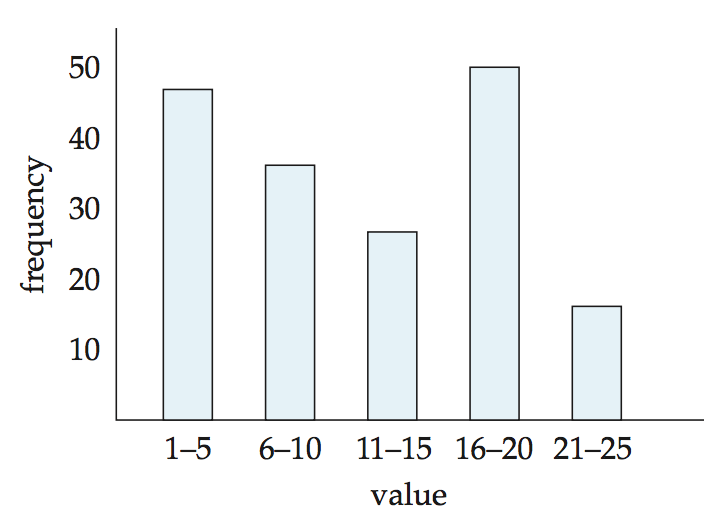
\includegraphics[width=0.4\textwidth]{images/histogram}
\end{center}

That should also tell you that they do not necessarily have an even distribution. A histogram does not take up a lot of space and it can help us to figure out certain problems: if we have a histogram of salaries and the largest bucket is 100~000+ and there are 10 people in this category, and there is a query asking how many employees have a salary greater than or equal to \$100~000 we will know at least that the number of tuples to be returned is 10. Nice.

The above numbers are exact values which we can know and, hopefully, trust although they could be slightly out of date depending on when exactly metadata updates are performed. The more exact values we have, the better our guesses. But things start to get interesting when, in the previous example, we ask something that does not have a category, such as how many people have a salary larger than \$150~000, where there isn't an obvious answer found in the metadata?

\subsection*{Join Elimination}

You may ask, of course, why should the optimizer do this work at all? Why not simply count on the developers who wrote the SQL in the first place to refactor/change it so that it is no longer so inefficient? That would be nice but would you also like a pony?  Developers make mistakes, as you know, or perhaps some legacy code cannot be changed for some reason. Regardless, SQL is a language in which you specify the result that you want, not specifically how to get it. If there is a more efficient route, then it's worth taking from the point of view of the database server. The same logic applies in the compiler, incidentally; if you ask for some operation that the compiler knows it can replace with an equivalent but faster operation, why wouldn't you want that? Compilers don't admonish the user for writing code that it has to transform into a faster equivalent, they just do that transparently. You're welcome!

Our guide in this is~\cite{joinelim}. We will examine some real SQL queries to see how we can get rid of a total unnecessary join. This join can only be removed if the database server can prove that the join is not needed and that therefore the removal of this operation has no impact on the outcome.


Consider a statement that looks like this: \texttt{SELECT c.* FROM customer AS c JOIN address AS a ON c.address\_id = a.address\_id;} This gets customer information and joins with those where there are addresses on file. This is an inner join and as presented, we cannot do any elimination with this information. We need to make sure that the customer data has a matching row.

If, however, a new piece of information is considered, it changes everything entirely. Suppose that we have a foreign key defined from customer's \texttt{address\_id} to the address \texttt{id} field. If nulls are not permitted then we know for sure that every customer has exactly one record in the address table and therefore the join condition is not useful and may be eliminated. This means we could in fact replace that query with \texttt{select * from customer;} with no need for any references to the join table at all. That would be much, much faster since it is a simple select with no conditions.

The foreign key and not null constraints on the address ID field of the customer make it possible for the optimization of the join elimination to occur.

An outer join constraint can be removed as well. Imagine the query said this: \texttt{SELECT c.* FROM customer AS c LEFT OUTER JOIN address AS a ON c.address\_id = a.address\_id;}. All tuples are fetched from customer whether or not there is an associated address. Once again, if the foreign key constraint and not-null properties hold for this field it means that we can perform the equivalent transformation and replace the join query with a simple unqualified select. 

Suppose the foreign key constraint is removed. Does that change anything? No -- a unique constraint on the address would be sufficient for us to conclude that the join means no duplication of rows in customer will take place. Therefore it can once again be replaced with the simple \texttt{select * from customer;}.

If, however, both constraints are removed and we cannot be sure that there is at most one address corresponding to a customer, then we have no choice but to do the join.

Obviously, the more complex the query, the harder it is to determine whether or not a particular join may be eliminated. More than that, the same queries written exactly the same on a database in which the constraints have not been added would not be eligible for the join elimination optimization. In the inner join example, the foreign key and not null constraints, for example, are beneficial. This reveals a second purpose why constraints are valuable in the database. In addition to allowing us to enforce logical rules of the application inside of the database, it allows queries to be completed more efficiently.

Perhaps an analogy helps. You are asked to search through the library to find all copies of the book ``Harry Potter and the pthread House Elves''. That is a plausible task. But, suppose that you know as well there is a rule that this library will keep only one copy of that book ever. If that is the case, as soon as you have found the single copy of that book, you can stop looking (no need to check more ``just in case''). This sort of optimization is very similar in that the rules let us avoid doing unnecessary work and that is a big part of the optimization routine.

\subsection*{Evaluation Plan Selection}

It was perhaps oversimplifying to have said earlier that choosing a plan was just as simple as picking the one with the lowest cost. There is a little bit more to it than that. The point about choosing the one with the lowest cost is correct (generally), but the difficulty is in devising and calculating all possible evaluation plans. Neither devising nor analyzing alternatives is free in terms of CPU usage or time, and it is possible to waste more time on analysis than a better plan would save. 

A simplified approach, then, focuses just on what order in which join operations are done and then how those joins are carried out. The theory is that the join operations are likely to be the slowest and take the longest, so any optimization here is going to have the most potential benefit.

We already know that the order of joins in a statement like $r_{1} \bowtie r_{2} \bowtie r_{3}$ is something the optimizer can choose. In this case there are 3 relations and there are 12 different join orderings. In fact, for $n$ relations there are $\dfrac{(2(n-1))!}{(n-1)!}$ possible orderings~\cite{dsc}. Some of them, are symmetric, which reduces the number that we have to calculate, since $r_{1} \bowtie r_{2}$ is not different from $r_{2} \bowtie r_{1}$ (in relational algebra). In any case, even if we can cut down the symmetrical cases the problem grows out of hand very quickly when $n$ gets larger. 

Once more than three relations are affected by a join query it may be an opportunity to stop and think very hard about what is going on here, because this is quite unusual if the database design is good. The database server may want to ask why do you have a join query that goes across six or eight or twelve relations, but the database server (sadly) does not get to write the developers a nasty resignation letter saying that it can't continue to work this hard due to the negative effects on its health. It will dutifully do the work you asked it to and even try to make the best of this inefficient situation by optimizing it. But clearly it cannot examine all (non-symmetric) approaches and choose the optimal one. It would take too long.

Fortunately, we can create an algorithm that can ``remember'' subsets of the choices. If we have, for example, $r_{1} \bowtie r_{2} \bowtie r_{3} \bowtie r_{4} \bowtie r_{5}$ and the database server does not segmentation fault in disgust, we can break that down a bit. We could compute the best order for a subpart, say $(r_{1} \bowtie r_{2} \bowtie r_{3})$ and then re-use that repeatedly for any further joins with $r_{4}$ and $r_{5}$~\cite{dsc}. This ``saved'' result can be re-used repeatedly turning our problem from five relations into two three-relation problems.

This is a really big improvement, actually, considering how quickly the factorial term scales up. The trade-off for this approach is that the resultant approach may not be globally optimal (but instead just locally optimal). If $r_{1} \bowtie r_{4}$ produces very few tuples, it may be maximally efficient to do that join computation first, a strategy that will never be tried in an algorithm where $r_{1}$, $r_{2}$, and $r_{3}$ are combined to a subexpression for evaluation. 

Remember though, this is as estimating process. The previous statement that said $r_{1} \bowtie r_{4}$ produces very few tuples as if it is a fact. The optimizer does not know that for sure and must rely on estimates where available. So even though the optimizer may, if it had tried all possibilities, determined that $r_{1} \bowtie r_{4}$ produces the fewest tuples and should be joined first, it is possible that estimate was off and the actual cost of a different plan was lower.

The sort order in which tuples are generated is important if the result will be used in another join. A sort order is called \textit{interesting} if it is useful in a later operation. If $r_{1}$ and $r_{2}$ are being computed for a join with $r_{3}$ it is advantageous if the combined result $r_{1} \bowtie r_{2}$ is sorted on attributes that match to $r_{3}$ to make that join more efficient; if it is sorted by some attribute not in $r_{3}$ that means an additional sort will be necessary~\cite{dsc}.

With this in mind it means that the best plan for computing a particular subset of the join query is not necessarily the best plan overall, because that extra sort may cost more than was saved by doing the join itself faster. This increases the complexity, obviously, of deciding what is optimal. Fortunately there are, usually anyway, not too many interesting sort orders~\cite{dsc}. 

\subsubsection*{Generating Alternatives}

Join order optimization is a big piece of the puzzle but it's not the only thing we can do in query evaluation. Let's briefly revisit the subject of how equivalent queries are formed. We already decided it is too expensive to try out all equivalent queries, but perhaps we are determined to try to at least generate lots of alternatives. The textbook~\cite{dsc} summarizes some strategies from the Volcano research project that would make it possible to generate a larger number of plans than we might otherwise be able to. We need four things.

\begin{enumerate}
	\item A way of storing expressions that reduces duplication and therefore keeps down the amount of space needed to store the various queries.
	\item A way of detecting duplicate derivations of the same expression.
	\item A way of storing optimal subexpression evaluation plans so that we don't have to recompute them.
	\item An algorithm that will terminate the evaluation of a particular plan early if it is already worse than the cheapest plan found so far.
\end{enumerate}

The details are obviously a bit complex. Most of this is beyond what we will discuss in this course, but some of those things we have already seen. For example, the algorithm earlier has got a way of storing evaluations of sub expressions so that we can re-use them. It could be modified to terminate earlier if, for example, the individual costs of \texttt{r1} or \texttt{r2} were already larger than the known stored plan.

\subsubsection*{Nested Subqueries}

On the subject of generating alternatives, if possible, nested subqueries will be transformed into an alternative representation: a join query. To summarize the rather long story, if evaluated the ``slow'' way the subquery needs to be run a lot of times. Thus, to make it faster, we would prefer to turn it into a join (which we already know how to handle). If really necessary we can run the subquery once and use that temporary relation in a join (where exists or ``in'' predicates may fall into this category).

Suffice it to say that transformation of nested queries is complicated and it may mean that the optimizer is unable to find some efficient route for executing the desired query if the query is complex. If possible, nested queries should be avoided. Sometimes you don't have much choice however. Amusingly, many years ago, MySQL did not support subqueries and that was one way to force people to come to grips with how to use joins. But somehow I do not think MySQL was intentionally doing anyone a favour, any more than having a terrible optimizer ``forces'' developers to write better queries. 


\subsubsection*{Shortcuts}

Now we will talk about some heuristic rules (guidelines, really) that we have definitely mentioned earlier when we talked about, for example, how to perform a selection. Now we can actually discuss them more formally.

\paragraph{Perform selection early.} No surprises here: the sooner we do a selection, the fewer tuples are going to result and the fewer tuples are input to any subsequent operations. Performing the selection is almost always an improvement. Chances are we get a lot of benefit out of selection: it can cut a relation down from a very large number of tuples to relatively few (or even one). 

There are exceptions, however. One from~\cite{dsc}: suppose the query is $\sigma_{\theta}( r \bowtie s )$ where $\theta$ refers only to attributes in $s$. If we do the selection first and (1) $r$ is small compared to $s$ and (2) there is an index on the join attributes of $s$ but not on those used by $\theta$ then the selection is not so nice. It would throw away some useful information and force a scan on $s$; it may be better to do the join using the index and then remove tuples with the selection.

\paragraph{Perform projection early.} Analogous to the idea of doing selection early, performing projection early is good because it tosses away information we do not need and means less input to the next operations. Just like selection, however, it is possible the projection throws away an attribute that will be useful. If the query does not ask for the join attribute in the output (e.g., does it matter what a person's address ID is?) then that join attribute will need to be removed from the output but if removed too soon it makes it impossible to do the join.

\paragraph{Set limits.} Another strategy for making sure we choose something appropriate within a reasonable amount of time is to set a time limit. Optimization has a certain cost and once this cost is exceeded, the process of trying to find something better stops. But how much time to we decide to allocate? A suggested strategy from~\cite{dsc} says to use some heuristic rules to very quickly guess at how long it will be. If it will be very quick then don't bother doing any further searching, just do it. If it will be moderate in cost, then a moderate optimization budget should be allocated. If it is expensive then a larger optimization budget is warranted.

\paragraph{Plan caching.} In any busy system, common queries may be repeated over and over again with slightly different parameters. For example, \cite{dsc} suggests the following sort of query: a student wishes to query what courses they are enrolled in. If one student does this query with a particular value for student ID number, we can re-use that same evaluation plan in the future when another student does the exact same query with her student ID number instead. 

The results will be different and this query may be more expensive on the second run if, for example, the second student is taking 7 courses this term and the first student is taking 5. That is expected, all we really needed was an estimate. With that in mind, if we have actually carried out the exact query we can use the actual execution time as the updated estimate for how long it takes (or perhaps an average of the last $n$ executions of that same query if it has high variability). 

\subsection*{Applicability}
If we're not planning on implementing or understanding a database, is any of this useful? Yes! The database is just a specific example of an implementation and something that we're familiar with. The real lesson is about how to programmatically generate, evaluate, and choose amongst alternative options for accomplishing a goal. 









\chapter*{20 --- Self-Optimizing Software}

\addcontentsline{toc}{chapter}{20 --- Self-Optimizing Software}

\section*{Self-Optimizing Software}
Our previous discussion about compiler optimizations (and optimizing the compiler) was focused on things that the compiler can do at compile-time. But what about runtime? The compiler can't do much at runtime, but a sufficiently-smart program can change itself at runtime to be better. Better, in this case, meaning faster. But what about change? We'll start with the simple things, and move on to the more complex  and harder to get right. The simple stuff has to do with changing what's in memory, and well advance into changing the configuration, and finally, we'll consider changing the binary itself.

\paragraph{Caching.} Your first thought about how a program might change itself for speed might be something like caching! Suppose that you keep track of the most popular exchange rates in memory, so that they are available faster than by going to the database. The management of the cache will be at runtime; the contents of the cache will be based on the actual usage. And, it will change over time to adapt to the patterns of usage: if today the exchange rate of CAD-EUR is popular, it will appear in the cache, and without any code changes if the exchange rate of CAD-GBP becomes popular, it goes in the cache and becomes faster to access. So, you \textit{do} technically get different behaviour at runtime, but this is not quite what we wanted to talk about in this topic. It's too easy, and your program should probably be doing it already.

\paragraph{Observe and change.}
The next idea relates to having your program's configuration change at runtime to adapt to observed behaviour. If there are multiple routes to the same outcome, we might decide at runtime which is the best. This is effective because our initial guess might not be correct, but also because conditions can change at any time. In Java, linked lists versus array lists are a quick example.

If you've taken a course in databases, you should have been exposed to the idea of query processing: given a certain query (\texttt{SELECT id FROM... JOIN... WHERE...}), the database server comes up with an execution plan for how to carry it out. For a simple query, there might be only one answer. A more complex query will have multiple correct answers and the database server will do what it considers best. However, that is based on an estimated cost only. The server could, at least once, try out a different strategy and notice if it is better than the original plan. A lot of queries happen many times (or are extremely similar to already-observed queries), so remembering what worked is helpful.

Building on that, the database server could change how it organizes the data based on what would be most efficient for the most common usage patterns. You can do the same in your program. For an analogy, I can sort the Excel sheet with student grades by either student ID (20xxxxxx) or user ID, based on whatever I use more. So if it is during the term and I'm entering grades, I probably use student ID as the way the file is sorted so I can get efficiently where I need to go. And I could always change that organization if it makes sense, such as after the end of term when people may e-mail me (including their user ID, but not student ID). The idea of re-structuring data storage can also apply to files on disk.

The observe-and-change strategy can also apply when invoking external services (external as in, over the internet). Suppose there are three different servers where we can send messages and we'll measure and remember how long it took to get a response from that server. The fastest server might be the one that is the closest geographically, but that server might be very busy, so it might be faster to communicate with a server that's less busy but farther away. Maybe you send 8 out of every 10 messages to the server that was most recently determined to be the fastest, and one to each of the other two servers. You might discover that your current guess at the fastest server is wrong and it's better to switch your primary.


\paragraph{Genetic algorithms.}
If you've taken an advanced course on algorithms, you might have covered genetic algorithms in some detail. This isn't going to be a replacement for that, but will just give you an idea of how the idea can be used. First, a quick three-paragraph explainer on genetic algorithms~\cite{genetic}.

A genetic algorithm is inspired by the idea of natural selection. Our program is trying to solve a particular problem. A number of candidate solutions are created (usually, randomly) and they are evaluated for their fitness: how well do they solve the problem? Solutions with a higher fitness have a higher chance of continuing forward into the next group of candidates, called the next generation. At each generation, good solutions from the previous generation are combined (if possible) and/or mutated randomly to see if that makes the solution better. This process repeats until a sufficiently-optimal solution is found, or a fixed number of generations have been evaluated. Thus, solutions with good qualities ``reproduce'' and move forward in the simulation, and those with bad qualities ``die out'' and we do not continue down that path. If we do this well, eventually we end up with a solution that's good, or at least good enough.

This works for the kind of problem where we, first of all, have some parameters to configure. If there is nothing to configure, there's nothing to change or evolve. We also need a fitness function that allows us to evaluate how well the problem is being solved. This function cannot be binary (pass/fail) because that doesn't show whether a given solution A is better or worse than solution B; instead we want a continuous or discrete (in the mathematical sense) definition of fitness so we can say solution A with 84.1 is better than B with 81.0.

Of course, a genetic algorithm does not necessarily guarantee the best possible outcome. It is possible that the fitness function tends towards a local maximum rather than the global one, so we get a good solution but not the best. Similarly, the fitness of a solution might be evaluated rarely or take a long time, making the process of finding a good solution slow.

Right, with that in mind, you might ask how genetic algorithms help in making your program faster. The typical use for a genetic algorithm is something like designing an antenna or an airplane wing where making random changes gives some numbers. We can do the same with a generic program, if it has the right properties and what we're trying to do is optimize our configuration parameters.

Let's return to the subject of Google Maps. In our earlier discussion on early-phase termination, we tried to brainstorm ideas about how potential routes are generated and how we know if we have enough or a good-enough route. In the discussion, we will imagine that the decision of when to terminate the search is based on when we have a ``good enough'' solution. Then there are the various parameters that go into generating a solution, which I'll guess to be something like:

\begin{itemize}
	\item Number of routes to evaluate
	\item Heuristic for generating routes to evaluate
	\item Decay of traffic information reported by other motorists
	\item Time of day and month and if it's a holiday
	\item Search radius for alternate routes
\end{itemize}

It is Google, after all, so they probably consider many more parameters or use a completely different mechanism. It might be very difficult to choose what the correct values for these parameters are (especially if they vary by time of day, day of the week, on holidays, etc). Changing them by hand probably does not work, but letting a genetic algorithm choose the values based on experimenting and trading off the quality of the solution against the time to come up with it. We might consider a solution that only comes up with awful routes to fail, even if it gets them nearly instantly. And we might consider the successful solution one that comes up with a route that is optimal or nearly-optimal in the shortest time.

One reason why genetic algorithms might be a good choice for this kind of problem is that the problem is nonlinear: that is, we cannot treat each parameter as an independent variable and change just one and expect that the change in output is only a result of the change of the one input variable and not also an interaction of one variable with others~\cite{genetic}.

Perhaps this takes away some of the mystery of genetic algorithms. Maybe you're thinking this isn't really self-optimizing software, it's just optimizing configuration parameters. Let's go up (well, really, down) a level, then. Now we'll move into changing the binary itself.

\paragraph{Hotspot.}
The previous discussion of compiler optimizations talked about all the things that compiler can do to make the program more efficient. Some of them are always a clear win. Precomputing something or skipping unnecessary code is always going to be better than the alternative. Other optimizations are not. Let's consider the decision about inlining: sometimes it's good, but sometimes it doesn't help or makes things worse. In those cases, the compiler has to take a decision about whether to do it or not and that's what is in the binary.

In JVM languages like Java, the virtual machine itself can do some optimization because of the just-in-time (JIT) compiler. The original program is turned into the intermediate representation by the Java compiler, and then there's a second chance at runtime! Oracle's documentation tell us that there's actually two different JIT compilers; one for clients and one for servers. The client one produces its output faster, but that code produced will be less efficient. The server one takes more time and more resources to produce slightly better code.

The major advantage that the JIT compiler has is being able to observe the runtime behaviour of the program and then change its decision. If we see that, for example, inlining would be helpful but the original decision was not to do it, we can change that decision. This is very helpful in scenarios like inlining, because we'll have the function call overhead every single time and therefore every call to the function increases the penalty of getting the decision wrong. Being able to change our decision is less helpful when it comes to something like a branch prediction, because the hardware will most likely save us if our prediction isn't very good (see our earlier discussion on this topic).

There are actually a few other things that can be done by the JIT compiler at runtime which are not likely to be doable at compile time. In particular, I want to focus on \textit{escape analysis} \textit{on-stack replacement}, and \textit{intrinsics} as outlined in~\cite{escape}.

Let's start with escape analysis. The purpose of this is to figure out if there are any side effects visible outside of a particular method. This allows some skipping of heap allocation and we can stack allocate them instead. The more interesting thing are possible lock optimizations: lock elision, lock coarsening, and nested locking. Lock elision: if the JIT compiler can determine that a lock serves no purpose---e.g., a method or block is tagged as \texttt{synchronized} but it can only ever get called from one thread at a time---there's no lock at all and therefore no setup or acquisition costs.  Lock coarsening: if there are sequential blocks sharing the same lock, the compiler can combine them to reduce the amount of locking and unlocking that needs to happen. The cuts down the overhead and we'll take it where we can. Nested locks: if the same lock is required repeatedly without releasing (in some recursive code, perhaps) this can also be combined so we don't have as much overhead lost to locking and unlocking.

On-stack replacement is a way that the virtual machine can switch between implementations of a particular method. This is helpful in that if a function is identified as important (sometimes called \textit{hot}) because it runs frequently, then a more optimized version can be swapped in. This does have a slight cost, in that the virtual machine has to pause execution briefly, potentially to recompile, and definitely to swap in the new stack frame (as it may be organized differently), but it will be of some benefit in the long run if this function is truly a frequently-executed piece of code.

If you've done debugging in a JVM language like Java or Kotlin you might have seen something like this in action! While you have the debugger attached, you can make changes, compile it, and the JVM will try to swap in the new code for the old code and continue running. This does not always succeed, but if it does it allows you to try a changed version of the program without having to stop and restart. That's particularly helpful when there's a long workflow to reproduce a particular problem and/or the application in question takes a long time to start up.

Intrinsics are highly-optimized versions of code, precompiled for a specific platform (e.g., x86). If a particular piece of code is truly critical, then using that native implementation might be faster, but it might not always be available, depending on your platform. These were originally developed in \CPP~rather than Java so it's also done without the safety rails of Java. I guess in that sense you could say that \CPP~ is Java's unsafe mode. That might be a controversial statement. Now there's a different approach called Graal, which turns the Java bytecode directly into machine code. Adding an intrinsic is a complicated process.

The hotspot approach is probably closest to what you might have imagined by reading the title of this topic: changing the binary code based on observed runtime behaviour of the program. Rust doesn't have the capability of detecting the parameters at runtime and swapping binary code them, because it has chosen not to have a runtime like the JVM. While that does mean that there's less overhead in general, the tradeoff is that any decisions made at compile time will remain so. Unless...

\paragraph{Rewriting the binary.}
Rewriting the binary in a language like C or Rust can happen, but requires us to do more work ourselves, or depend on a library that implements that functionality for us.

One possibility is to have different versions of a compiled block of code at the ready. That is, we direct the compiler, when the program is being built, to make several variants of the same code with different optimization decisions or other tradeoffs. We'll start with a default, and if we determine based on some observation that we need to change, then overwrite that part of the binary in memory with the new version and we've changed the code path that executes!

There are a couple difficulties that that approach, though. Yes, it increases compile time, but that's usually acceptable as a tradeoff, and is of minor concern. The first big question is how many variants of the code will you compile and have prepared? This is still compile-time work so we're not sure what the real data and behaviour will be like at runtime, so we are still guessing, but we get multiple guesses instead of just one. Then we have to make sure a section of code isn't being executed when we want swap it out, but that's possible to do with some locking mechanism or other software coordination.

That approach is rewriting the binary at run-time, but you might be thinking that if it's all precompiled anyway, can't we decide at runtime with if-statements what function to call to get the same effect? I think so, and thus we haven't really reached the real goal which is doing it truly dynamically. Which is an option.

So, you want to compile your own code. With our understanding of all the things the compiler does, you can reasonably assume that you're not going to write your own and include it in your program. Code generation isn't magic or so incredibly difficult that you can't do it, but if you want to make optimal code you need a lot of the analytics and decision-making that's in the compiler. So the only realistic way of getting the code compiled is to use an existing compiler, that is, the one that's already on the target system.

Requiring a specific compiler on the target system might limit your ability to actually deploy this technique. For one thing, if it's end-user software, they might not have compilers installed at all (Windows?), or if they do it's a different compiler (LLVM vs gcc, perhaps)? And you might also encounter a security policy on your servers that forbids the installation of a compiler to make it harder for any exploit that somehow works its way in to compile and run its payload.

If we can actually use the compiler on the target system, then we are in business. The approach is simple to explain if somewhat complicated in practice. First, take the binary code of the segment that we want to optimize and then have the compiler take a look at it. The compiler will then take the binary, convert it to its internal representation (the intermediate representation), then optimize it, and compile it. The new binary code can get swapped in when it's ready.

On top of the advantage of having runtime information when compiling this time, this kind of approach also makes it possible to inline or rewrite library functions if we want. The amount of benefit will vary a lot based on the library. Some are pretty efficient as-is, but others with lots of functionality might benefit a lot by being optimized for the one use-case you need.

Does this work? Yes; here's some research on the subject from~\cite{binaryrewriting}. They are doing a calculation on a matrix of size 649 $\times$ 649 for 20~000 iterations. Here's their graph of the performance results from the improved code:

\begin{center}
	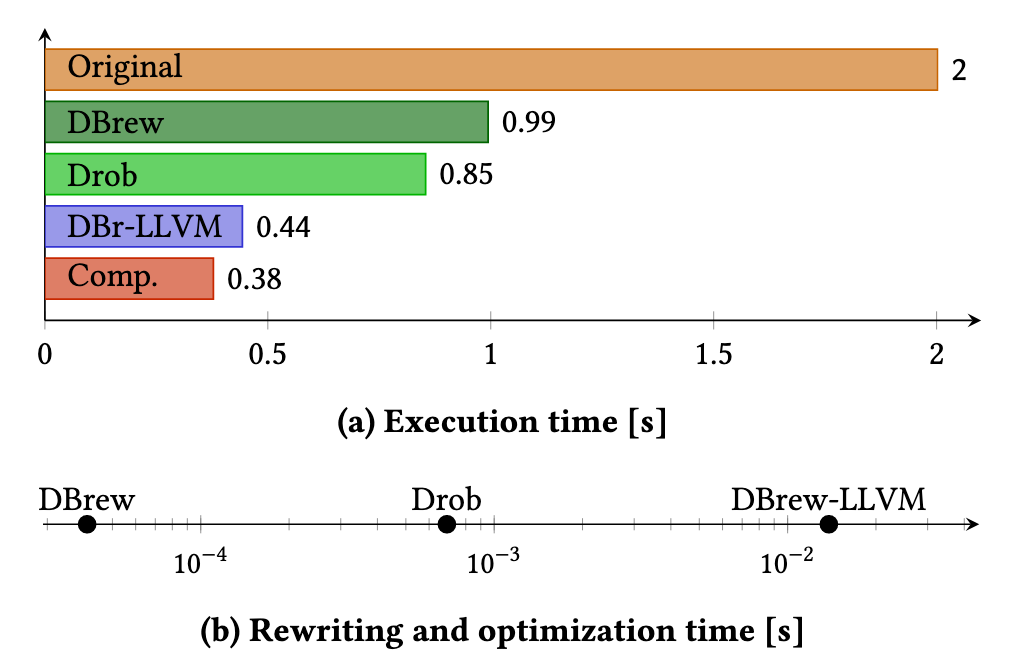
\includegraphics[width=0.6\textwidth]{images/rewriting.png}
\end{center}

As expected, there is a significant cost associated with the process of recompiling a segment of the program. But given the right workload, there is clearly a benefit in the execution time of the updated program. In that case, this is worth doing on code that will run frequently.

\paragraph{Program sus.}
It's worth noting that programs that rewrite themselves are frequently judged as suspicious by anti-virus and anti-malware software. The story behind this is a part of a software arms race. It starts with the first viruses, which are malicious code doing malicious things. So, anti-virus software is developed to detect viruses and the primary mechanism for detecting if something is a virus is comparing the binary code under examination against a database of malicious software.

To combat this binary-matching pattern, some viruses will alter themselves in subtle ways or produce code that's functionally equivalent but looks different in binary than the original. A virus is not usually something that requires excellent performance, so making a transformation that's slower but looks different to the virus scanner is fine (from the villain point of view, anyway).

It's impossible to predict all possible transformations for a particular piece of software, because there's a lot of routes to the same destination. Anti-virus software can try to ignore things like inserted NOPs or pay no attention to variables X and Y being swapped and then swapped back to just add some assembly instructions. Still, an alternative approach that some anti-virus programs choose is heuristic analysis, which is analyzing broadly what the program under examination does and seeing if its behaviour looks... suspicious.

Combining those two facts means that a benign program that changes its own binary code might be considered by anti-virus software to be suspicious and prevented from running or otherwise restricted in some way. If you're determined to rewrite the binary, just keep in mind that anti-malware software end-users have installed may affect the experience (if you are, in fact, shipping to end-users at all).








\chapter*{21 --- Performance Case Study, Performance Culture}

\addcontentsline{toc}{chapter}{21 --- Performance Case Study, Performance Culture}

\section*{Making Firefox Fast}

Let's look at Mike Conley's Firefox Performance Updates,
\begin{center}
{\scriptsize
\vspace*{-1em}
\url{https://mikeconley.ca/blog/2018/02/14/firefox-performance-update-1/}
}
\end{center}
\vspace*{-1em}

\begin{itemize}[noitemsep]
\item don't use CPU animating out-of-view elements
\item move db init off main thread
\item keep better profiling data
\item parallel painting for macOS
\item lazily instantiate Search Service only when first search starts
\item halve size of the blocklist
\item refactor to reduce main-thread IO
\item don't hold all frames of animated GIFs/APNGs in memory
\item eliminate an unnecessary hash table
\item use more modern compiler
\end{itemize}

We can categorize most of these updates into the categories we've seen before:
\begin{itemize}[noitemsep]
\item do less work (or do it sooner/later);
\item use threads (move work off main thread);
\item track performance;
\end{itemize}
Which of the updates fall into which categories?

\subsection*{Tab warming} We continue by examining one particular update, \emph{tab warming}, in detail:
\begin{center}
\scriptsize
\vspace*{-1em}
\url{https://mikeconley.ca/blog/2018/01/11/making-tab-switching-faster-in-firefox-with-tab-warming/}.
\end{center}
\vspace*{-1em}

\hfill ``Maybe this is my Canadian-ness showing, but I like to think of it almost like coming in from shoveling snow off of the driveway, and somebody inside has \emph{already made hot chocolate for you}, because they knew you’d probably be cold.'' --- Mike Conley

Consider switching tabs. Previously, Firefox would request a paint of the newly-selected tab and wait for the rendering to be available before switching the tab.

The idea is to reduce user-visible latency by predicting an imminent tab switch. How do you know that the user is about to switch tabs? When the user has a mouse, then the mouse cursor will hover over the next tab.

\begin{quote}
Assuming a sufficiently long delay between hover and click, the tab switch should be perceived as instantaneous. If the delay was non-zero but still not long enough, we will have nonetheless shaved that time off in eventually presenting the tab to you.

And in the event that we were wrong, and you weren’t interested in seeing the tab, we eventually throw the uploaded layers away.
\end{quote}

The blog post does not report performance numbers (but bug 1430160 discusses how to collect them).

\subsection*{Firefox in general}

Try: ``about:mozilla'' in Firefox. On a Quantum Flow-enabled version, you'll see

\begin{center}
\emph{The Beast adopted new raiment and studied the ways of Time and Space and Light and the Flow of energy through the Universe. From its studies, the Beast fashioned new structures from oxidised metal and proclaimed their glories. And the Beast’s followers rejoiced, finding renewed purpose in these teachings.}

\hfill \emph{from The Book of Mozilla, 11:14}
\end{center}

In 2017, Mozilla released Electrolysis (E10s)~\cite{electrolysis}.
which leverages multicore processors by using multiple OS-level
processes. (Chrome has always done this, but Firefox attempts to also
keep memory usage
down~\cite{goldilocks}.
Beyond internal architecture issues, handling Add-Ons (now
WebExtensions) was perhaps the most challenging part of going
multi-process.

Note the connection to different thread/process models.
Chrome is one-process-per-tab, while Firefox multiplexes tabs across
the 4 content processes (``hardware threads'', by analogy). Limiting
the number of tabs also limits the memory consumption of the browser:
we don't have arbitrary numbers of renderer state.

\begin{center}
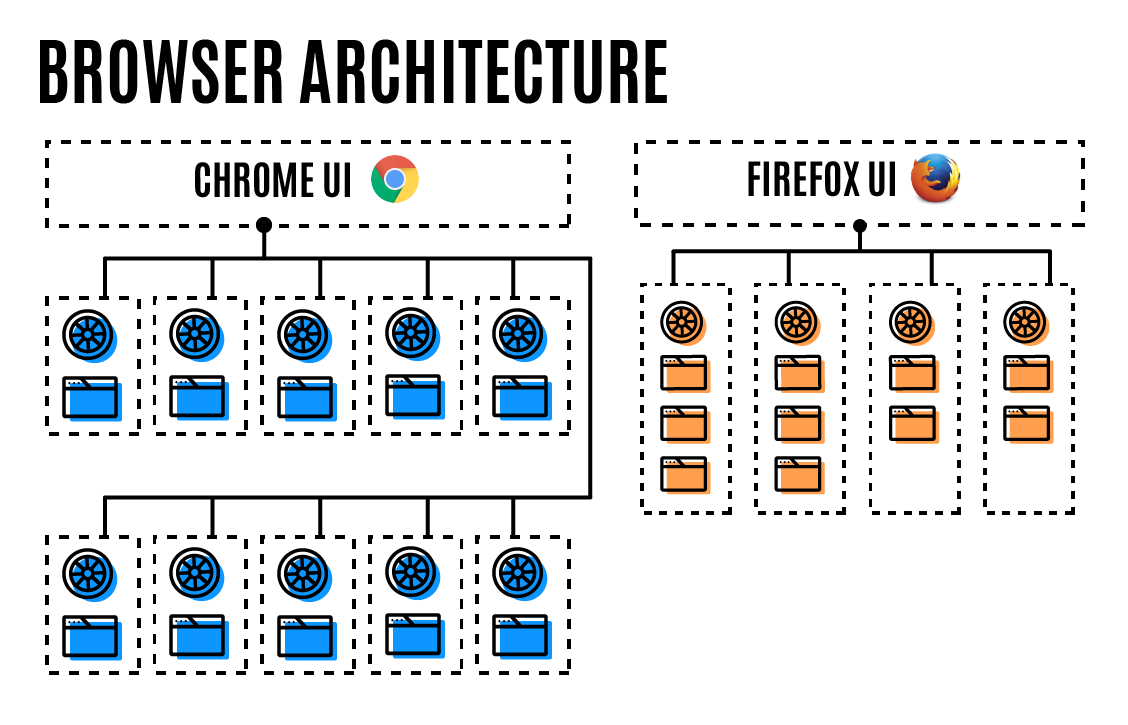
\includegraphics[width=.9\textwidth]{images/L19-chrome-vs-firefox.png}
\end{center}
Source: Ryan Pollock~\cite{goldilocks}

As a crude summary, Electrolysis works on splitting across processes
while the newer Quantum Flow leverages multithreading and other
improvements.  Quantum Flow uses the Rust programming language and its
``fearless concurrency'' (in Rust-speak). We used to say that Rust should probably be part of a future revision of the ECE 459 curriculum. The future is now! But our focus is on Firefox.

\subsection*{Quantum Flow}
Here's a retrospective of the Quantum Flow project:
\begin{center}
\url{https://ehsanakhgari.org/blog/2017-09-21/quantum-flow-engineering-newsletter-25}
\end{center}

To sum up, they formed a small team and did the following.
\begin{enumerate}[noitemsep]
\item Measure slowness: gather information, instrument Firefox, collect profiling data and measurements. Prioritize issues.
\item Gather help: convince other teams to pitch in with perf improvements. Examples: front-end team (reduce flushes, timers); layout team (reflow performance).
\item Fix all the things! (Or at least the most important ones).
\end{enumerate}
Given the short timeline they gave themselves (6 months) and the limited resources, an important part of their work was convincing others to help.
They triaged 895 bugs and fixed 369 of them. The weekly Quantum Flow Engineering Newsletter was a key motivational tool.

After the project wound down, they aimed to distribute responsibility for perf improvements across the entire project.

\section*{Firefox Telemetry}
Firefox's Telemetry feature collects lots of information from Firefox
users.  Idea: collect data before hacking away at things.  Firefox collects hundreds of
gigabytes of anonymous metrics per day while browsing and makes it all available to
the public.  One can view this as an analogy of CPU profiling on a
massively distributed context. This data is collected much less often than
CPU profiling data but at a much broader scope.
\begin{center}
\url{https://telemetry.mozilla.org/}
\end{center}
If you are running Firefox and want to see what it is collecting:
\begin{center}
\url{about:telemetry}
\end{center}

You can view distributions of telemetry probes (in the form of
histograms). You can also make your own dashboard based on Firefox
Telemetry data and Mozilla has infrastructure for their developers to
formulate and evaluate their own queries.

Example questions:
\begin{itemize}[noitemsep]
\item Is Firefox the user's default browser? (69\% yes)
\item Does e10s make startup faster? (no, slower)
\item Which plugins tend to freeze the browser on load? (Silverlight and Flash)
\end{itemize}
Can see evolution of data over time.

Firefox developers can propose new telemetry probes which are reviewed
for data privacy\footnote{Mozilla Data Collection Practices: \url{https://wiki.mozilla.org/Firefox/Data_Collection}} as well as through normal code review channels.

\paragraph{Pings.} Firefox phones the data home using so-called ``pings''.
Firefox sends a ``main ping'' every 24 hours, upon shutdown, environment change,
and crash. There are other types of pings as well. Pings get sent either by Firefox
or by a helper program, Pingsender, when Firefox isn't running. Presumably they
are sent over the network as compressed JSON to a central server.

Here's the common ping structure:

{\scriptsize
\begin{verbatim}
{
  type: <string>, // "main", "activation", "optout", "saved-session", ...
  id: <UUID>, // a UUID that identifies this ping
  creationDate: <ISO date>, // the date the ping was generated
  version: <number>, // the version of the ping format, currently 4

  application: {
    architecture: <string>, // build architecture, e.g. x86
    buildId: <string>, // "20141126041045"
    name: <string>, // "Firefox"
    version: <string>, // "35.0"
    displayVersion: <string>, // "35.0b3"
    vendor: <string>, // "Mozilla"
    platformVersion: <string>, // "35.0"
    xpcomAbi: <string>, // e.g. "x86-msvc"
    channel: <string>, // "beta"
  },

  clientId: <UUID>, // optional
  environment: { ... }, // optional, not all pings contain the environment
  payload: { ... }, // the actual payload data for this ping type
}
\end{verbatim}
}

Pings contain scalars (counts, booleans, strings) and histograms. A histogram collects
bucketed data (think grade distributions). Both scalars and histograms can be keyed, e.g.
how often searches happen for which search engines.

\section*{Laws of Performant Software}

Suppose you want to write fast programs and you like checklists and handy rules. If so, you are in luck, because there is Crista's Five Laws of Performant Software~\cite{lpsw}. 

\paragraph{1. Programming language $<<$ Programmers' awareness of performance.}
There is no programming language that is magic, whether good or evil. All the major programming languages allow you to write programs that perform well or badly. 

There's a lot of C-elitism in the world, and then there's the back-in-my-day-sonny people who claim assembly was best, and they also had to walk to school in the snow, uphill both ways.  High level languages give you lots of options... Do I use an array? A vector? A list? And yes, some of the fancy tools you get are syntactic sugar: they are convenient from the programmer's point of view, but what do they do behind the scenes? If the performance is not what you expect, there is probably be a better way to do it in the high level language.

I'll add my own asterisk on this rule: some languages lend themselves better to parallelization than others. A language may force a certain way of thinking, based on its rules (e.g., functional programming languages). But there is no reason why the way of thinking can't be applied in another language.


\paragraph{2. $d(f^{\tau}(x), f^{\tau}(y)) > e^{\alpha\tau} d(x, y)$ or small details matter.} This complicated formula is from the butterfly effect (chaos theory). If two versions of the code are $x$ and $y$, the difference between the performance outcomes $f(x), f(y)$ is much larger than the difference between the code.

A small code change can have a huge impact. Did you fix a memory leak? The addition of one \texttt{free()} call is a single line code change but can, in the long run, have a dramatic impact on performance. Is caching used properly? Can you use a faster serialization algorithm? 

Basically: don't overlook the small stuff. It's tempting to think that huge major architectural changes are the solution to everything; but there are plenty of gains to be found in the small things.

\paragraph{3. corr(performance degradation, unbounded resource usage) > 0.9.}
There is a very high correlation between performance degradation and unbounded use of resources. Often times we focus on functionality: the software must have the following 847~251 features! But if you want a program that scales you need to think in terms of operation, not functionality.

Resources need to be limited. If there aren't hard limits, eventually a resource will be exhausted. If the program starts threads, use a thread pool and the thread pool should have a fixed size. Is there a cache? It needs a maximum size. If you need to read input, don't use a function that reads an entire line (of arbitrary length). Furthermore your program needs design effort given to what happens when resources are exceeded. So you decide to set a request queue size; once that queue is full, further requests are rejected in some well-understood manner. 

\paragraph{4. Performance improvements = log(controlled experiments)}
If you want your code to be faster you have to know why it is slow. It's okay not to know the answers, but not knowing how to find out is a problem. Don't guess; measure.


\paragraph{5. N*bad != good.}
No amount of nodes, cores, memory, etc, will save you from poorly-written code. Throwing more hardware at the problem is expensive and ineffective in the long term. Bad code is still bad no matter how much hardware it runs on. 

\section*{Performance Tips}

While we're on the soapbox, a few more small things to note from~\cite{preopt} about how one might write code in a performant as well as maintainable way.

\paragraph{Understand the order of magnitude that matters.} If you are writing code where 100 CPU cycles matters, then a function that will acquire a lock through some sort of shared-memory interlocked instruction then this instruction is performance murder. And it might be even worse if lock acquisition fails and you get blocked for 100~000 cycles trying to acquire the lock... On the other hand, if you have a network intensive then the 100 cycle stuff does not matter even the smallest bit because it is lost in the noise of the network.

\paragraph{Plan for the worst case scenario.} I don't mean for the nuclear apocalypse, as much fun as that might be. As~\cite{preopt} wrote:

\begin{quote}
What happens if that lock is held for longer than expected, because the system is under load and the scheduler is overloaded? And what if the owning thread was preempted while holding the lock, and now will not get to run again for quite some time? What happens if the network is saturated because a big news event is underway, or worse, the phone network is intermittently cutting out, the network cable has been unplugged, etc.? What about the case where, because a user has launched far too many applications at once, your memory-intensive operation that usually enjoys nice warmth and locality suddenly begins waiting for the disk on the majority of its memory accesses, due to demand paging? These things happen all the time.

In each of these situations, you can end up paying many more orders of magnitude in cost than you expected under ordinary circumstances. The lock acquisition that usually took 100 CPU cycles now takes several million cycles (as long as a network roundtrip), and the network operation that is usually measured in milliseconds is now measured in tens of seconds, as the software painfully waits for the operation to time out. And your ``non-blocking'' memory-intensive algorithm on the UI thread just caused a hang, because it's paging like crazy.
\end{quote}

No doubt you have seen these sorts of things as well and it is an awful user experience. The spinning beach ball of death and the ``Not Responding'' added to the title bar are all symptoms of this situation. 

\paragraph{Acknowledge and plan for asynchrony.} A quick example from~\cite{preopt}: suppose that Jordan is writing code to return a list of fonts to be used in the UI. The code checks a local font cache, and if that is already initialized, returns the fonts found in the cache in a List object. If the cache is not initialized, however, the data needs to be loaded, perhaps from the printer (which will dutifully tell you what fonts it can print out). Morgan intends to use this list of fonts in the UI of the program but is unaware that in certain circumstances this call will take much longer (that is, when the cache is not initialized).

Supposing that the API just returns a \texttt{List<Font>}, it is not obvious to Morgan where these come from. And in local testing on the dev machine with nothing on it and nothing else doing and the printer is always turned on, and rainbows and unicorns are present. Thus even if the cache is not initialized it is ``fast enough''. But in the real world, of course, the printer will be down and unicorns are nowhere to be found and it runs up against some hard timeout of 20 seconds. 

If, however, Jordan's API now has a return type of \texttt{Task<List>} (generify as desired), then it is obvious to Morgan that there is something asynchronous going on here at least some of the time. With this information in hand, the UI won't wait for this task and we might even convince Jordan to give us partial results (so we can draw the UI elements as backing data arrives) or at the very least, a progress bar. Users love progress bars. They are wildly inaccurate and not super informative even if they are accurate, but at least they give the user the impression that something is happening.

That actually leads us down a side debate about how to make the program appear faster than it is by some UI trickery and psychological ``hacks'', but that is beyond what we want to talk about here...

\section*{Performance Culture}

Now let's take it up a level: how do you make performance an important aspect of the culture of development of a project. The source for this section is~\cite{perfculture}.

The author's recommendations of warning signs that performance culture is off the rails:

\begin{itemize}
\item Answering the question, ``how is the product doing on my key performance metrics,'' is difficult.
\item Performance often regresses and team members either don't know, don't care, or find out too late to act.
\item Blame is one of the most common responses to performance problems (either people, infrastructure, or both).
\item Performance tests swing wildly, cannot be trusted, and are generally ignored by most of the team.
\item Performance is something one, or a few, individuals are meant to keep an eye on, instead of the whole team.
\item Performance issues in production are common, and require ugly scrambles to address (and/or cannot be reproduced).
\end{itemize}

As tempting as it is to say these are all technical issues, they are really human problems. It would obviously be preferable to start with a good performance culture in the first place, but that is not always going to happen. But suppose you are already in a hole. The usual course of action is to stop and say to yourself ``I appear to be in a hole... I know, I'll dig my way out!''. Maybe I am cynical. The right thing to do would be stop digging, of course...

Change has to come from both the top down and the bottom up. Management needs to make performance a priority: ask questions, demand rigour... while at the same time, people doing the development need to understand the performance of what they write, making practice improvements. Both sides need to have zero tolerance for regression.

If only one person is responsible for performance, this will not work. One person could not reasonably keep up with the rest of the team. If the other developers don't have performance in mind when writing, it would mean the key performance person would spend unnecessary time rewriting things when the it could have been right in the first place. If this isn't convincing, think about unit tests. Could you really ``outsource'' the writing of all unit tests to one person? And would code quality be the same if you did?

The author is very adamant that poor performance culture is management's fault. Managers need to budget time, reward the work, and encourage performance work. Managers who don't understand performance culture are likely to be caught by surprise and blame things. 

Consider the following comparison from~\cite{perfculture}:

\begin{quote}
Manager A gives lip service to performance culture. She, however, packs every sprint schedule with a steady stream of features -- ``we've got to crush competitor Z and must reach feature parity!'' -- with no time for breaks in-between. She spends all-hands team meetings praising new features, demos aplenty, and even gives out a reward to an engineer at each one for ``the most groundbreaking feature.'' As a result, her team cranks out features at an impressive clip, delivers fresh demos to the board every single time, and gives the sales team plenty of ammo to pursue new leads. There aren't performance gates and engineers generally don't bother to think much about it.

Manager B takes a more balanced approach. She believes that given the competitive landscape, and the need to impress customers and board members with whizbang demos, new features need to keep coming. But she is also wary of building up too much debt in areas like performance, reliability, and quality for areas she expects to stick. So she intentionally puts her foot on the brake and pushes the team just as hard on these areas as she does features. She demands good engineering systems and live flighting of new features with performance telemetry built-in, for example. This requires that she hold board members and product managers at bay, which is definitely unpopular and difficult. In addition to a reward for ``the most groundbreaking feature'' award at each all-hands, she shows charts of performance progress and delivers a ``performance ninja'' award too, to the engineer who delivered the most impactful performance improvement. Note that engineering systems improvements also qualify!
\end{quote}

But this is a startup, you object, why does it matter, because we need the minimum viable product and we needed it yesterday, and also, VCs like features. Well maybe, but architecture matters. There's time to fix things later, maybe, but you can really cripple your startup by choosing the wrong things early on. 

After a discussion of the why and the what, it is time to think about how to make it systematic. If it is not systematic, it will not get done and it will be dropped when in a time crunch. And development teams are always in a time crunch! This is why best practices have automated unit tests that run on every commit (or at least build). And much the same way, there need to be performance tests; if something has significantly regressed performance, the build failed and the commit is no good. This obviously requires that the tests be meaningful, testing effectively and not overly noisy. 

Performance tests may be a bit too large and difficult to run for every commit or every build. Although it would be nice to know exactly which commit is the cause of the problem, you may want a test that runs overnight to see the long term trends. And thus a 12-hour test is probably unsuitable for this. The solution is, obviously, levels of test. 

One company I [JZ] worked for did something like this, although it was not performance specific. Before committing to the CVS repository (at this point nobody had heard of git) there was a set of tests called ``precheckin''. Nobody forced a developer to run it, but you were definitely supposed to, and it just verified that everything would compile and some basic stuff worked. These tests took a few minutes to run. Then each build on the build server had a larger set of tests (``build''), including the precheckin material and a lot more, taking about 30-40 minutes to execute. Breaking this breaks the build (and gets everyone's attention). Then there were the ``regression'' tests that ran overnight (and ALL night).

\cite{perfculture} advocates zero tolerance rules: anything that significantly regresses performance is reverted and re-worked. No exceptions, no questions, no pleading one's case, etc. If exceptions are allowed, exceptions quickly become the rule, and promises to fix something later are procrastinated endlessly.

Obviously when code does more it should be expected to take longer, but then the test(s) should be adjusted as well. This is the same as when developing new features/changes, after all; unit tests are adjusted when code changes are introduced intentionally.

\paragraph{Metrics} There are, roughly speaking, two categories of metrics:

\begin{itemize}
	\item \textit{Consumption}: measure resources consumed by running a test.
	\item \textit{Observational}: measure the outcomes of running the test, from the view of outside the system.
\end{itemize}

Consumption metrics are the things that we can easily measure about the code run during the test: cache misses, TLB misses, context switches, number of I/Os, memory allocated, number of system calls (traps are interrupts, remember). Observational metrics are more along the lines of time it takes to run a dataset, or number of work items processed per unit time, etc.

It might seem like observational metrics are all that we care about. End users care about the amount of time it takes to complete their work, or management/sales/marketing/C-levels care about the throughput and that's it. This matters, sure, but it's not enough to know the outcome; the consumption metrics are necessary to break down why the total time (or throughput) is what it is.

Suppose a change is committed and the tests run and the total time it takes increases by 10\%. If that's all you know, you know that things got worse but have no data as to why. You can obviously read the source code or the diff and try to look for it, but even that might not tell you enough. If you see that memory allocations are reported and you have now allocated more memory than before,  at least you have a theory to start with on what's slowing down the code. It might not be that, it might be something else entirely, but it's a place to start. Memory allocation changes are relatively easy to spot though: there's a new call to \texttt{malloc} or a structure has been extended in some way. If it is a cache miss issue, finding that without the data is harder...

Does this remind you of \texttt{printf} debugging? It's a little bit like that. But then again, you want to use this sort of thing for long running tests anyway. If the test is going to run for 4h it would be helpful to know where exactly in that four hours it went off the rails (on a crazy train!). 

There's one more consideration and that is the variability between runs. In the ideal situation, there is consistent performance every run. That is probably too much to ask for and there will be some natural variation due to nondeterminism in computers. But a change that causes a wild change in the variance is also no good; a test that sometimes finishes in 0.5$\times$ time and sometimes in 2$\times$ time has a high variance and this will not be acceptable. 

Be ready to dig deep: suppose a developer has introduced a change that is slow under rare circumstances. Those rare circumstances are not triggered until $n$ years later when a second developer introduces another change. The second change will be identified, at least initially, as the ``problem''. There's two ways to go about it; either fix the initial change or work around it. Which one is correct will depend very much on the circumstances, but at the very least both options should be considered. It's not about blame or not about fault; it's about improving the performance of the software.










\chapter*{22 --- GPU Programming (CUDA)}

\addcontentsline{toc}{chapter}{22 --- GPU Programming (CUDA)}

\section*{GPUs: Heterogeneous Programming}

The next part will be about programming for heterogeneous
architectures. In particular, we'll talk about GPU programming, as
seen in CUDA. The general idea is to
leverage vector programming; vendors use the term SIMT (Single
Instruction Multiple Thread) to describe this kind of
programming. We've talked about the existence of SIMD instructions
previously, but now we'll talk about leveraging SIMT more
consciously. We are again in the domain of embarrassingly parallel
problems.

\paragraph{Cell, CUDA, and OpenCL.} 
Other examples of heterogeneous programming include
programming for the PlayStation 3 Cell~\cite{cellprimer} architecture and CUDA. (Note that the PS4 returns to a regular CPU/GPU configuration; however, it uses AMD hardware which combines the CPU and GPU on one chip.) The Cell includes a PowerPC core as well as
8 SIMD coprocessors:

\begin{center}
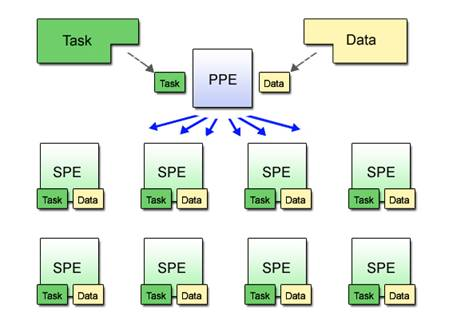
\includegraphics[width=.4\textwidth]{images/cell.jpg}
\end{center}
\hfill (from the Linux Cell documentation)

CUDA (Compute Unified Device Architecture) is NVIDIA's architecture
for processing on GPUs. ``C for CUDA'' predates OpenCL; NVIDIA still
makes CUDA tools available, and they may be faster than OpenCL on NVIDIA
hardware. On recent devices, you can use (most) \CPP~features in CUDA code,
which you can't do in OpenCL code. We used to teach OpenCL, but it seems
to be the case that CUDA has found widespread acceptance out in industry.
Hence, we use CUDA in the course. If you really need cross-platform or 
you have AMD hardware, then you want OpenCL. The principles are similar 
enough that you can take what you learned in one toolchain and apply it 
to the other.

\paragraph{Programming Model.} The programming
model for all of these architectures is similar: you write the code for
the massively parallel computation (kernel) separately from the main
code. Then at run-time, set up the data (input), transfer the data to the GPU, wait while the GPU executes the kernel, then transfer the results back. 

It makes sense to hand it over to the GPU because there are a lot of cores, although they run at a slower speed when compared to the CPU. Looking at the hardware in the ECE servers as of Fall 2020, ecetesla2 has a 4 core 3.6 GHz CPU. It also has 1920 CUDA cores that run at about 1.8 GHz. So, half the speed, but 480 times the workers. Sounds like we could get quite some speedup... if the workload is suitable.

At run-time, there is significant set-up cost for interacting with the GPU and then the data transfers (input to the GPU and collecting the results) mean there is a significant overhead cost for using the GPU. But the GPU can do lots of work in parallel once it gets going. This is a lot like deciding whether to drive or fly. 

If the distance is short, say, 200 km (the distance between Ottawa and Montreal) then flying makes no sense: you have to get to the airport, be there at least an hour or two early to make your way through security checkpoints, then fly, then get from the destination airport to your final destination. Sure, the flying part is fast, but the overhead makes your total average speed not worth it.

On the other hand, if you're going a longer distance, like 4000 km (roughly the distance between Waterloo and San Francisco), then driving is way slower! Sure, the overhead of going the airport remains, but once you're in the air you're moving at 800 km/h or so and in 5.5 hours you are there. Compare that to 40 hours of driving.

CUDA includes both task parallelism and data parallelism, as we've
discussed earlier in this course. \emph{Data parallelism} is the central
feature. You are evaluating a function, or \emph{kernel},
at a set of points. Each point represents a data element, such as one of the
bodies in the n-body simulation. But you could also perform some 
transformation on each pixel of an image or each frame of a video. If you 
imagine a 2-dimensional problem, each little circle in the diagram below is
a work-item:

\begin{center}

\begin{tikzpicture}
\foreach \x in {0,0.25,...,2}
  \foreach \y in {0,0.25,...,2}
    \draw (\x, \y) circle (0.25mm);
\end{tikzpicture}
\end{center}

Another name for the set of points is the \emph{index space}. 
Each of the points corresponds to a \emph{work-item}.

CUDA also supports \emph{task parallelism}: it can run different
kernels in parallel. Such kernels may have a one-point index space. This is
doing a large number of different things in parallel. We're not really going
to focus on that and will instead stick to the part about data parallelism.

\paragraph{More on work-items.} The work-item is the fundamental
unit of work. These work-items live on an $n$-dimensional
grid (ND-Range); we've seen a 2-dimensional grid above. You may choose
to divide the ND-Range into smaller work-groups, or the system can
divide the range for you. CUDA spawns a thread for each work item,
with a unique thread ID; they are grouped into blocks. Blocks can share 
memory locally, but each block has to be able to execute independently.
That is, the system can schedule the blocks to run in any order and possibly
in parallel (we hope so!). 

You get your choice about block size. Usually, we say let the system decide. However, for some computations it's better to specify; if you do, however, you want to make best use of the hardware and use a multiple of the size of the \textit{warp}. A warp is the NVIDIA term for a unit of execution, and there can be multiple units of execution in a given GPU.

\paragraph{Shared memory.} CUDA makes lots of different types of
memory available to you:

\begin{itemize}
\item private memory: available to a single work-item;
\item local memory (aka ``shared memory''): shared between work-items
  belonging to the same work-group; created by the compiler and includes values spilled from registers and small arrays declared inside kernels~\cite{micikevicius11:_local_memor_regis_spill}
\item global memory: shared between all work-items as well as the host;
\item constant memory: resides on the GPU, and cached. Does not change.
\item texture memory: this is global memory too, also cached, and it provides potentially a very slight speedup over using global memory. The GPU has texture memory and caches that it uses for rendering and interpolating textures, and it's available for the GPU's general-purpose operations if your use case is a match. 
\end{itemize}

Choosing which kind of memory to use is an important design decision. A simple kernel might put everything in global memory, but that's likely to be slower than making good use of local memory. It could also be tempting to put all unchanging data in the constant memory, but its space is limited, so giant vectors won't always fit.

There is also host memory (RAM in your computer), which generally contains the application's data. We will be doing explicit transfers of the data from host memory to the GPU memory, in both directions.

\paragraph{My very own Kernel.} Let's start looking at a kernel. This is the code that will be executed by every CUDA thread somewhat in parallel. First, let's see what the code would look like if we just wrote it in \CPP:

\begin{lstlisting}[language=C++]
void vector_add(int n, const float *a, const float *b, float *c) {
  for (int i = 0; i < n; i++) {
    c[i] = a[i] + b[i];
}
\end{lstlisting}


The same code looks like this as a kernel~\cite{cuda}:
\begin{lstlisting}[language=C++]
__global__ void vector_add(float* A, float* B, float* C)
{
    int i = blockIdx.x;
    C[i] = A[i] + B[i];
}
\end{lstlisting}

We can see in this example that there's no more loop. This is because the loop has become implicit. The loop induction variable here is something we retrieve from \texttt{threadIdx.x} --- the thread index. The index is a three-component vector so it has x, y, and z dimensions. For this one-dimensional (linear) problem, we only need the first component (x). We'll come back to multi-dimensional problems later.

You can write kernels in a variant of \CPP, and it looks mostly like the language we (hopefully) know, with a few additions like the \texttt{\_\_global\_\_} designation in the previous example. A large number of features of more recent versions of the language are supported, but how much will vary based on your release of the kernel compiler (\texttt{nvcc}). There's a list of things that are not allowed in device code. It's unlikely that we'll be doing too many things that are exotic enough to be forbidden by the compiler, in this course. However, if you aren't sure why something isn't working or want to know what kind of stuff is not allowed, see \url{https://docs.nvidia.com/cuda/cuda-c-programming-guide/index.html#restrictions}. We might mention some restrictions if we encounter any in thing to write example kernels.

The kernel itself is compiled into a form called PTX -- Parallel Thread eXecution -- instructions. It's possible to write those directly, but we won't; we'll just let the compiler do it. In theory, as with assembly instructions, it might be possible for an expert to produce better PTX instructions than the compiler does, but let's assume we're not. Also, using the \texttt{nvcc} compiler makes it so your kernel will run on whatever hardware you have. Just as you would when compiling in another language, it's advised to recompile if you change machines (e.g., uploading to ECE servers from your laptop, or switching from one ECE server to another).

The \texttt{nvcc} compiler has specific requirements for the underlying compiler it relies. At the time of writing, the default \texttt{gcc} works on \texttt{ecetesla[01234]}, so that you can use the command \texttt{nvcc -ptx nbody.cu}.
%For example, on \texttt{ecetesla2} at the time of writing, \texttt{nvcc} fails without specifying \texttt{gcc} version 6 instead of the default. With the command \texttt{nvcc --compiler-bindir /usr/bin/gcc-6 -ptx nbody.cu}, it will compile. 

Remember that the kernel has none of the safety guarantees that we normally get in Rust! We can easily read off the end of an array, forget to initialize a variable, allocate memory that we forget to deallocate, or have race conditions, amongst other things. All things that Rust normally prevents. So, not only can you encounter runtime errors in your kernel, but also, it's wise to check that your output matches expectations rather than just assume it's fine. It's even more true here that, just because it compiles, there are no guarantees that it will work.

If you want a quick example of what can go wrong with the kernel at runtime, here's something I got in testing:
{\scriptsize
\begin{verbatim}
thread 'main' panicked at 'Failed to deallocate CUDA Device memory.: IllegalAddress', 
/home/jzarnett/.cargo/registry/src/github.com-1ecc6299db9ec823/rustacuda-0.1.2/src/memory/device/device_buffer.rs:259:32
note: run with `RUST_BACKTRACE=1` environment variable to display a backtrace
thread 'main' panicked at 'Failed to deallocate CUDA Device memory.: IllegalAddress', 
/home/jzarnett/.cargo/registry/src/github.com-1ecc6299db9ec823/rustacuda-0.1.2/src/memory/device/device_buffer.rs:259:32
stack backtrace:
\end{verbatim}
}

\paragraph{More complex kernel example.} Here's a kernel we wrote for an N-body problem. It is just a straightforward brute-force approach (we could approximate to make it go faster, and that was a previous Lab 4):

\begin{lstlisting}[language=C++]
__device__ void body_body_interaction(float4 point1, float4 point2, float3 *acceleration) {
    float4 difference;

    difference.x = point2.x - point1.x;
    difference.y = point2.y - point1.y;
    difference.z = point2.z - point1.z;
    difference.w = 1.0f;

    float distSqr = difference.x * difference.x + difference.y * difference.y + difference.z * difference.z + 1e-10;

    float distSixth = distSqr * distSqr * distSqr;
    float invDistCube = 1.0f / sqrtf(distSixth);

    float s = point2.w * invDistCube;

    acceleration->x += difference.x * s;
    acceleration->y += difference.y * s;
    acceleration->z += difference.z * s;
}

extern "C" __global__ void calculate_forces(const float4* positions, float3* accelerations, int num_points) {
    if (blockIdx.x >= num_points) {
        return;
    }
    float4 current = positions[blockIdx.x];
    float3 acc = accelerations[blockIdx.x];

    for (int i = 0; i < num_points; i++) {
        body_body_interaction(current, positions[i], &acc);
    }
    accelerations[blockIdx.x] = acc;
}
\end{lstlisting}

Let's break it down. The calculation of forces between bodies takes some \texttt{float4} and \texttt{float3} arguments. In the Rust example, I made my own \texttt{Point} and \texttt{Acceleration} types. CUDA uses \textit{vector types}, which are a group of $n$ of that primitive type. So a \texttt{float4} is a grouping of four \texttt{float}s where the components are referred to as \texttt{x, y, z, w}. There exist vector types for the standard C primitives (e.g., \texttt{int, uint, float, double, char}, and some more) in sizes of 1 through 4. It's just a nice way to package up related values without needing a custom structure (although you can send structures in to kernels). When we get to the host code you'll see that I've had to modify its representation of the data as well.

The function also is prefixed with \texttt{\_\_device\_\_} which indicates that it will be called from another function when running on the GPU. A \texttt{\_\_global\_\_} function (as the calculation of forces is called from the host, and such global functions can call device functions but not other global functions. Device functions can call only other device functions. So it makes it clear where the entry points are from host code. In some OOP-sense, you could consider the device functions to be ``private'', not that I encourage you to think that way.

The only other thing that really stands out is the \texttt{extern "C"} declaration at the beginning of the global function. This disables what is called \textit{name mangling} or \textit{name decoration}, which is to say a compiler trying to differentiate between multiple functions with the same name. If this is too compiler-magic to worry about, just place this magic spell in front of the function call and it prevents the compiler from telling you it can't find the function by the name you specified. More modern versions of \texttt{nvcc} may not have this problem, mind you.

We'll also be using the N-body kernel soon as an example for when we examine how to launch a CUDA program. Also, if you're curious, the compiled version of the kernel resembles assembly language. The output is a little too large to show in the notes/slides, but the compiled version is in the course repository.

\subsection*{Writing a Kernel Well}

To start with, of course, we need to decide what sort of work belongs in the kernel to begin with. Anything that would benefit from the very large number of execution units is a good candidate, so that's typically things that are the iterations of a loop. If the loops need to be sequential, though, this is not a good use of the parallelism. If you need a little bit of coordination, we can achieve that, though, with barriers (similar to the concept as seen in concurrency). 

Comparing the first kernel that we saw against its CPU-code equivalent, we've taken the explicit for loop and made it implicit as a one-dimensional problem. We just use the GPU on the outer loop. What if we wanted to make it a two-dimensional problem? We could instead treat each pair of points $(i, j)$ as a point in the space, making it a two-dimensional problem. Then you could think of it as a matrix rather than an array and provide it to CUDA like that. This might increase the parallelism! 

Although that sounds good, for the N-body problem, it's not. The calculation of body-body interaction for just one pair of points is a very small amount of work, tiny even. Having one work-item for each such calculation means there's a lot of overhead to complete the calculation and it doesn't make sense. But if the calculation of the interaction were more complex, then this transformation might be an improvement.

We can also have three-dimensional problems. If you want something more than a three-dimensional, you have to have some loops in your code. So that 6-level-deep nested-for-loop? You can have the outer three loops as your x, y, and z dimensions, but the rest will be in for loops. Can't avoid everything, I am afraid. The limit to three dimensions is probably because graphics cards were designed for rendering images in 3-D so it seems logical? But that's only a guess.

Of course, you can sometimes flatten the dimensions of your problem a bit. A rectangular array in C/\CPP~is really stored as a linear array and the \texttt{[x][y]} is just notational convenience so you could easily just treat it as a linear array. If that's the case, you can avoid the need for a loop in your code. In the N-Body problem, having more items of smaller size is not an improvement because they're too small to be meaningful. Maybe a different problem would have different characteristics.

Consider something like brute-forcing a password of 6 characters (easy, but just for the purpose of an example). A one-dimensional approach might generate (in host code) one starting possibility for each valid character in the first position and then let the kernel loop over all possible other values. Then you might be able to improve that by generating starting possibilities in a 3-D matrix for the first three positions and loop in the kernel after that. Whether this is better or not is something that needs testing. And then one could think about generating more starting possibilities by flattening another dimension. It might be faster if it allows more things to be checked in parallel, but it might be slower because of the extra time spent generating the initial conditions in the host code. And eventually at some point (when there are longer passwords), there are too many possibilities to reasonably fit in the host code memory and it becomes impractical to transfer them to and from the GPU.

Of course, this isn't necessarily the best way to brute-force a password. We'll return to that subject later!

\paragraph{Branches.} CUDA implements a SIMT architecture. The documentation warns you, however, that unlike a CPU, there's neither branch prediction nor speculative execution. This means that branches are much more costly than they would be on the CPU. 

In practice, the hardware will execute all branches that any thread in
a warp executed (which can be slow). It then keeps only the results that are valid. Consider this brief example:

    \begin{verbatim}
__global__ void contains_branch(float *a, float *b) {
    if (condition()) {
        a[blockIdx.x] += 5.0;
    } else {
        b[blockIdx.x] += 5.0;
    }
}
\end{verbatim}

In the above example, the {\tt if} statement will cause
the warp both branches of the {\tt if}, keeping only the
result that is correct. But still, unnecessary work is done. It won't be possible to avoid all conditional branches, but they get expensive quickly.

Similarly, executing a loop will cause the
workgroup to wait for the maximum number of iterations of the loop in
any work-item. The compiler will try to unroll loops if they have a known number of iterations. Here, an example from the CUDA docs of a loop it can unroll:

{\scriptsize \hspace*{2em} \begin{minipage}{.5\textwidth}
    \begin{lstlisting}
__device__ void foo(int *p1, int *p2) {
  for (int i = 0; i < 12; ++i) {
    p1[i] += p2[i]*2;
  }
}
    \end{lstlisting}
\end{minipage} }

\paragraph{Atomic functions.}

We also mentioned earlier that there's still the possibility of race conditions. This means that if you want to, say, concurrently add to the same location, you need to use atomic functions. The atomic operations are usable on the standard primitive types like integers, floating point numbers, etc. And there are atomic operations for adding, subtracting, min, increment, decrement, as well as compare-and-swap and bitwise operations. Here's a quick example from the docs on a compare-and-swap~\cite{cuda}:

\begin{lstlisting}[language=C++]
__device__ double atomicAdd(double* address, double val) {
    unsigned long long int* address_as_ull =
                              (unsigned long long int*)address;
    unsigned long long int old = *address_as_ull, assumed;

    do {
        assumed = old;
        old = atomicCAS(address_as_ull, assumed,
                        __double_as_longlong(val +
                               __longlong_as_double(assumed)));

    // Note: uses integer comparison to avoid hang in case of NaN (since NaN != NaN)
    } while (assumed != old);

    return __longlong_as_double(old);
}
\end{lstlisting}

\subsection*{Launch?}

So far, all we have covered is the theory and then how to write a kernel. To make use of it, we'll have to look at the host code. That's our next topic. 










\chapter*{23 --- GPU Programming Continued}

\addcontentsline{toc}{chapter}{23 --- GPU Programming Continued}

\section*{GPUs: Heterogeneous Programming}

\section*{Host Code}
We've learned about how a kernel works and a bit about how to write one. The next part is the host code. Now, fortunately, we don't have to write the whole program in \CPP~ or C, even though the kernel has to be written in the CUDA variant. We're going to use the Rustacuda library from \url{https://github.com/bheisler/RustaCUDA}. That allows us to write code in Rust that interfaces with the GPU, and we can limit the interactions with unsafe code as much as possible.
 
We'll look at a quick example of launching a very simple kernel from the Rustacuda examples\footnote{\url{https://github.com/bheisler/RustaCUDA/blob/master/examples/launch.rs}}: 
\begin{lstlisting}[language=Rust]
#[macro_use]
extern crate rustacuda;

use rustacuda::prelude::*;
use std::error::Error;
use std::ffi::CString;

fn main() -> Result<(), Box<dyn Error>> {
    // Set up the context, load the module, and create a stream to run kernels in.
    rustacuda::init(CudaFlags::empty())?;
    let device = Device::get_device(0)?;
    let _ctx = Context::create_and_push(ContextFlags::MAP_HOST | ContextFlags::SCHED_AUTO, device)?;

    let ptx = CString::new(include_str!("../resources/add.ptx"))?;
    let module = Module::load_from_string(&ptx)?;
    let stream = Stream::new(StreamFlags::NON_BLOCKING, None)?;

    // Create buffers for data
    let mut in_x = DeviceBuffer::from_slice(&[1.0f32; 10])?;
    let mut in_y = DeviceBuffer::from_slice(&[2.0f32; 10])?;
    let mut out_1 = DeviceBuffer::from_slice(&[0.0f32; 10])?;
    let mut out_2 = DeviceBuffer::from_slice(&[0.0f32; 10])?;

    // This kernel adds each element in `in_x` and `in_y` and writes the result into `out`.
    unsafe {
        // Launch the kernel with one block of one thread, no dynamic shared memory on `stream`.
        let result = launch!(module.sum<<<1, 1, 0, stream>>>(
            in_x.as_device_ptr(),
            in_y.as_device_ptr(),
            out_1.as_device_ptr(),
            out_1.len()
        ));
        result?;
    }

    // Kernel launches are asynchronous, so we wait for the kernels to finish executing.
    stream.synchronize()?;

    // Copy the results back to host memory
    let mut out_host = [0.0f32; 20];
    out_1.copy_to(&mut out_host[0..10])?;
    out_2.copy_to(&mut out_host[10..20])?;

    for x in out_host.iter() {
        assert_eq!(3.0 as u32, *x as u32);
    }

    println!("Launched kernel successfully.");
    Ok(())
}
\end{lstlisting}

And the kernel it corresponds to is\footnote{\url{https://github.com/bheisler/RustaCUDA/blob/master/resources/add.cu}}:
\begin{lstlisting}[language=C]
extern "C" __constant__ int my_constant = 314;

extern "C" __global__ void sum(const float* x, const float* y, float* out, int count) {
    for (int i = blockIdx.x * blockDim.x + threadIdx.x; i < count; i += blockDim.x * gridDim.x) {
        out[i] = x[i] + y[i];
    }
}
\end{lstlisting}

\paragraph{Walk-through.} Let's look at all of the code in the example and
explain the terms. For a more detailed explanation of all the steps, see~\cite{cuda}.

One thing that we won't see is any explicit call to initialize the runtime. The CUDA runtime is automatically initialized when there's the first call into it. Thus, the first call might report errors that you wouldn't expect from that call, because they are really a setup problem on your system.

Right, in the example, we need to include the prelude for Rustacuda, just as we've seen previously for Rayon. This imports a bunch of commonly used types to save on having a lot of imports. 

First thing we have to do is initialize the API. This has to happen at the start of the program, so no sense in delaying it! At present, there are no flags defined so the call with \texttt{CudaFlags::empty()} is the only valid argument to the initialization function. 

Then we get a \textit{device}. The device is your graphics card or any other hardware that does the work. It's obviously possible to have more than one compute device, but we'll just take the first one. 

Next, in step 3, we request a \emph{context}. The context is described by the documents as analogous to a process. When we launch something within that context, it executes in there and has its own address space, and when the context is destroyed, all its resources are cleaned up. Each host thread may have one context. The call shown is ``create and push'' because a host thread has a stack of current contexts. We don't actually need the context for any of the later steps, but we just need to be in possession of one. In this simple example, it stays in scope because everything happens in \texttt{main}. If you want more structure to your program, then you do have to ensure it doesn't go out of scope and get dropped, because it has to exist for the other functions to work. When it does get dropped, some cleanup actions take place, of course.

The next step is to create our \textit{module}. A module is technically a package of code and data to run on the device, but in this case it just really means our kernel. What we do here is read the compiled PTX code into a C-String, then create the module from that string. It's also possible to load from a file directly. 

Once we have created a module, we then create a \textit{stream}. The stream is where we assign work. You can think of it as being similar to a priority queue: you put items in there and work that is more important (lower priority number) can pre-empt work that is less important (higher priority number). Otherwise, work is done in the order it was scheduled, and tasks don't overlap. The stream is asynchronous, so once work has been assigned, it returns immediately. I'll point out that the Rustacuda implementation says you should set the \texttt{NON\_BLOCKING} flag to prevent synchronization with the NULL stream (the details of which we'll skip). 

There's one more step before launching the kernel; in step 5, we
create some \emph{data buffers}, which are used for moving data to and from the GPU. Remember, CUDA requires explicit communication, so whatever data want to provide as input has to be put into a buffer and then the buffer is transferred to the kernel. Whatever data comes as output will be transferred by the GPU into the output buffers we specify.

After all this setup, we can finally launch the kernel. This has to be done in an \texttt{unsafe} block, because the launch macro is unsafe (unfortunately). The good news is that the unsafe block is only the launch, limiting the area of extra scrutiny to something small. When we launch, we specify the kernel that's supposed to run as well as the arguments. Each buffer is converted using the \texttt{as\_device\_ptr()} so that the contents of the device buffer are provided. For scalar types like the count, no such conversion is necessary and we can just provide the value. Here, we specify the grid size and block size (1 each). We'll be returning to that subject a bit.

Great! We launched the kernel and sent it over to the GPU. This is an asynchronous process, so we could do more stuff here if we need. There's nothing else to do at the moment, so we'll wait for the items in the queue to complete by calling \texttt{stream.synchronize()}. Straightforward!

Finally, in the last step, we copy the items out of the buffer and back into host memory. Here, the example code checks that all the values are correct (3.0) and it is! Alright, we have a simple working example of how to setup, launch, and collect results from a CUDA computation!

\subsection*{N-Body Host Code}

Here's the corresponding host code for the N-Body problem where we saw the kernel last time. A lot of it will be the same as the example code, but there are some differences that are noteworthy. Let's get started.

\begin{lstlisting}[language=Rust]
#[macro_use]
extern crate rustacuda;
extern crate rustacuda_derive;
extern crate rustacuda_core;

use cuda_sys::vector_types::{float3, float4};
use rustacuda::prelude::*;
use std::error::Error;
use std::ffi::CString;
use rand::Rng;
use rustacuda_core::DeviceCopy;
use std::ops::Deref;

/* A Rustification by Jeff Zarnett of a past ECE 459 N-Body assignment that was
originally from GPU Gems, Chapter 31 and modified by Patrick Lam.
Then CUDA-fied by Jeff Zarnett using the Rustacuda library example code
 */

const NUM_POINTS: u32 = 100000;
const SPACE: f32 = 1000.0;

struct CudaFloat4(float4);
unsafe impl DeviceCopy for CudaFloat4 {}
impl Deref for CudaFloat4 {
    type Target = float4;

    fn deref(&self) -> &Self::Target {
        &self.0
    }
}
struct CudaFloat3(float3);
unsafe impl DeviceCopy for CudaFloat3 {}
impl Deref for CudaFloat3 {
    type Target = float3;

    fn deref(&self) -> &Self::Target {
        &self.0
    }
}

fn main() -> Result<(), Box<dyn Error>> {
    // Set up the context, load the module, and create a stream to run kernels in.
    rustacuda::init(CudaFlags::empty())?;
    let device = Device::get_device(0)?;
    let _ctx = Context::create_and_push(ContextFlags::MAP_HOST | ContextFlags::SCHED_AUTO, device)?;

    let initial_positions = initialize_positions();
    println! {"Initial positions:"}
    for pt in initial_positions.iter() {
        println! {"({}, {}, {}) [{}]", pt.x, pt.y, pt.z, pt.w};
    }
    let mut accelerations = initialize_accelerations();

    let ptx = CString::new(include_str!("../resources/nbody.ptx"))?;
    let module = Module::load_from_string(&ptx)?;
    let stream = Stream::new(StreamFlags::NON_BLOCKING, None)?;

    // Create buffers for data
    let mut points = DeviceBuffer::from_slice(initial_positions.as_slice())?;
    let mut accel = DeviceBuffer::from_slice(accelerations.as_slice())?;

    unsafe {
        // Launch the kernel with one block for each point, with 1 thread each, no dynamic shared memory on `stream`.
        let result = launch!(module.calculate_forces<<<NUM_POINTS, 1, 0, stream>>>(
            points.as_device_ptr(),
            accel.as_device_ptr(),
            points.len()
        ));
        result?;
    }

    // Kernel launches are asynchronous, so we wait for the kernels to finish executing.
    stream.synchronize()?;

    // Copy the results back to host memory
    accel.copy_to(&mut accelerations)?;

    println! {"Accelerations:"}
    for a in accelerations.iter() {
        println! {"({}, {}, {})", a.x, a.y, a.z};
    }
    Ok(())
}

fn initialize_positions() -> Vec<CudaFloat4> {
    let mut result: Vec<CudaFloat4> = Vec::new();
    let mut rng = rand::thread_rng();

    for _i in 0..NUM_POINTS {
        result.push(CudaFloat4 {
            0: float4 {
                x: rng.gen_range(0.0, SPACE),
                y: rng.gen_range(0.0, SPACE),
                z: rng.gen_range(0.0, SPACE),
                w: rng.gen_range(0.01, 100.0),
            }
        });
    }
    result
}

fn initialize_accelerations() -> Vec<CudaFloat3> {
    let mut result: Vec<CudaFloat3> = Vec::new();
    for _i in 0 .. NUM_POINTS {
        result.push(CudaFloat3 {
            0: float3 {
                x: 0f32,
                y: 0f32,
                z: 0f32,
            }
        });
    }
    result
}
\end{lstlisting}

We mentioned last time that in the kernel we can use vector types like \texttt{float4}. If we want to use those in Rust, we have to import them from a library (here cuda-sys) that isn't the same as the Rustacuda library\footnote{So at the time that I wrote this, I actually submitted an issue in the Rustacuda library to bring in support for this. Maybe by the time you are reading this, support has been added. I might even have found time to do it myself, should I finish all the course content and have time.}. This gives us the \texttt{float4} but there's a requirement of the Rustacuda library that any type that we want to send over to the kernel must have the trait \texttt{DeviceCopy}. Implementing the trait is promising that the type you have does not contain any pointers to host memory (so if you had a struct that contained a pointer to a buffer, this is not okay). That's because the pointer will be bogus when it is on the GPU device (they don't share memory). I also added the \texttt{Deref} trait which makes it so that the array of this type \texttt{CudaFloat4} will be easily converted to the type it contains \texttt{float4} when we operate on it. And the same for the \texttt{float3} type.


The other thing worth noting is that the calculation of forces kernel is invoked with a grid size of \texttt{NUM\_POINTS} and one thread per block. That is to say, there are \texttt{NUM\_POINTS} (100~000) chunks of work, and each chunk has one thread. If you get this wrong, the code doesn't work as expected: if you put in 1 and 1 for both of these values, then only the first acceleration will be calculated, because we said there's one chunk of work and it's one thread. But what we actually have asked for is to have \texttt{NUM\_POINTS} chunks and that will get it done.

When done, we copy the data out and print it and we're done! Below that, you can also see there's a little change to how the initial values are created in that we have to set the content of the \texttt{CudaFloat3/4} through parameter 0. 

\paragraph{Putting it to the test.}
That's great, but how much does it speed up? I ran this on ecetesla1 (because my laptop does not have the correct graphics card for this purpose), so I reran all the CPU benchmarks to have a fair comparison for what happens on the same machine. With 100~000 points:
\begin{itemize}
	\item \texttt{nbody} (sequential, no approximations): 40.3 seconds\vspace{-1em}
	\item \texttt{nbody-parallel} (parallel, no approximations): 5.3 seconds\vspace{-1em}
	\item \texttt{nbody-cuda} (parallel, no approximations): 9.5 seconds
\end{itemize}

Hey, wait a minute. That's worse than the CPU version. Uh, what's wrong here? My first theory was that 100~000 points is not enough to overcome the overhead of setup and transferring data to and from the device. This turned out to be incorrect (and it was painful to try the sequential version with more points). 

Eventually, I used a profiler (we'll come back to profiling shortly) and it told me that most of the time was going to the kernel execution of the \texttt{calculate\_forces} function. This convinced me that the problem was that I wasn't getting the most out of the GPU as I could be. I don't think there was anything terrible about the kernel itself, but I really wanted to go back to the question of the grids and blocks. Here's a (sadly terrible quality) image from the CUDA docs that explains it~\cite{cuda}:
\begin{center}
	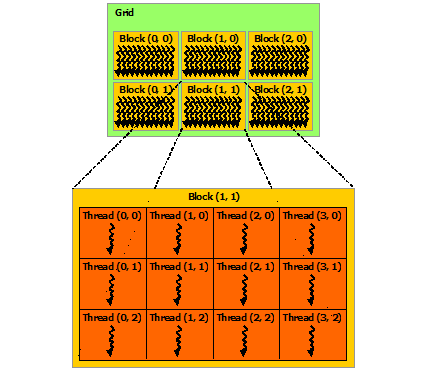
\includegraphics[width=0.5\textwidth]{images/grid-of-thread-blocks.png}
\end{center}

The documentation isn't super great about how grids and blocks work, unfortunately, and a lot of the guidance on the internet says is ``experiment and try'' (so helpful). The initial approach that I wrote had each work-item be its own block. That's inefficient, because we're not taking advantage of all the hardware that's available (the warp hardware). The advice that I can find says the number of threads per block should always be a multiple of 32 with a maximum of 512 (or perhaps 1024 with more modern devices). The second guidance I can find is that numbers like 256 and 128 are good ones to start with, and you can tweak it as you need. Then you have to adjust the grid size: divide the number of points by the threads per block to give the number of blocks. Here's the improved call:

\begin{lstlisting}[language=Rust]
        let result = launch!(module.calculate_forces<<<(NUM_POINTS/256) + 1, 256, 0, stream>>>(
            points.as_device_ptr(),
            accel.as_device_ptr(),
            points.len()
        ));
        result?;
\end{lstlisting}

I did have to add a +1 to the number of blocks, because 100~000 does not divide evenly by 256, and if you forget that then the last few of the accelerations are all zeros. But just running it as-is didn't work (and led to the kernel crashing). Why? Because the indexing strategy that I used contained only the reference to the block index \texttt{blockIdx.x}. That's fine in the scenario where every work-item gets its own block, but that's no longer the case now: 256 work-items (points) now share each block. Here's the adjusted kernel the calculates the correct index. 

\begin{lstlisting}[language=C++]
extern "C" __global__ void calculate_forces(const float4* positions, float3* accelerations, int num_points) {
    int idx = threadIdx.x + blockIdx.x * blockDim.x;
    if (idx >= num_points) {
        return;
    }
    float4 current = positions[idx];
    float3 acc = accelerations[idx];

    for (int i = 0; i < num_points; i++) {
        body_body_interaction(current, positions[i], &acc);
    }
    accelerations[idx] = acc;
}
\end{lstlisting}

The full version of the improved code is in the course repository as \texttt{nbody-cuda-grid}. But what you want to know is, did these changes work? Yes! It sped up the calculation to about 1.65 seconds (still with 100~000 points, still on the same server). Now that's a lot better! We are finally putting the parallel compute power of the GPU to good use and it results in an excellent speedup.









\chapter*{24 --- Password Cracking, Bitcoin Mining}

\addcontentsline{toc}{chapter}{24 --- Password Cracking, Bitcoin Mining}

\section*{GPU Application: Password Cracking}

GPUs are good---too good, even---at password cracking. We'll discuss a paper
that proposes a technique to make it harder to crack passwords. This technique
is scrypt, the algorithm behind DogeCoin~\cite{scrypt}. See also \url{http://www.tarsnap.com/scrypt.html}

First, let's talk about acceptable practices for password storage. It is \emph{not}
acceptable engineering practice to store passwords in plaintext. The inevitable security
breach will end with your company sending a ``sorry'' disclosure email to its clients,
and you will be responsible for the ensuing bad publicity. Acceptable practices: {\bf not} plaintext; hashed and salted (we won't discuss salting here but hopefully you remember it from previous courses or other experience.)

\paragraph{Cryptographic hashing.} Instead of storing the plaintext password, you
store a hash of the password, under a cryptographic hash function. One important
property of a cryptographic hash function is that it must be (believed to be a) one-way
function; that is: $x \mapsto f(x)$, the forward direction, must be easy to compute, but
$f(x) \mapsto x$, the inverse mapping, must be hard to compute. Examples of such functions
include SHA-3 and scrypt. 

Some known cryptographic algorithms are already pretty well broken (DES, SHA1) and if you choose one of those then it's like no security at all. Other systems have a broken implementation of the algorithm that is vulnerable to some attack. And even if you chose a good algorithm with no known vulnerabilities in the implementation, you need to choose enough bits (e.g., 512 and not 32), otherwise it's too easy to break...

\paragraph{Not Secret.}
In real life, you can get around the idea of cryptographic hashing by looking on the internet to see if someone's password has already been leaked. Many services are terrible about their password storage policies so if you used the same username and password combination of mycrappywebsite.com and your online banking, then if the mycrappywebsite database gets hacked then the attacker has your user and password already without having to break anything.

\paragraph{First, Check if the Door Is Locked}
As you might imagine, the first thing to try is super common passwords: ``password'', ``system'', et cetera. Users frequently choose common words as passwords and if you just try them all you might get a hit. Choose stronger passwords!

\paragraph{Breaking the hash.} Even if there is no known short computation for the
inverse function, it's always possible to brute-force the password
computation by trying all possible passwords. Think about how GPUs
work. Each potential password is a point in the computation space, and
we compute the hash over all of them simultaneously.  That's a lot of
speedup.

Any website with even slightly decent design will start locking accounts after too many bad login attempts, if not outright banning the caller. But if you get a copy of the database, or at least of some cryptographically-hashed passwords, then a brute force approach is possible.

\paragraph{Arms race: making cracking difficult.} The idea has always been
to make it more difficult to compute the hash function. This does make it longer for the user when they want to log in, but the amount of time to compute a single password is reasonable. However, it's intractable to try all possible passwords, at least with current hardware. 

Even way back,
UNIX passwords forced repeated applications of the hash function to increase the difficulty. The computational power available to us today is of course dramatically more than it was 20 or 30 years ago, and we can reasonably imagine that the computational power in 20 years will vastly exceed what we currently have, making it plausible to crack a password that's effectively uncrackable today. That's okay, just make sure to change your encryption algorithm (and your password!) as needed to stay ahead of the crackers.

Aside: quantum computing won't basically wreck everything we're talking about in virtually zero time. Those are really good for solving problems like asymmetric key encryption (e.g., RSA), but not as good at hashing problems. Fortunately for our banking details.

The main idea behind scrypt is to make hashing expensive in both time and space,
increasing both the number of operations and the cost of brute-forcing. This is how we increase the difficulty to make it implausible to crack in a reasonable amount of time. The only choice that they have to try to break it is, well, to use more circuitry to break passwords (and it will take more time).

Of course, there's always this form of cracking:
\begin{center}
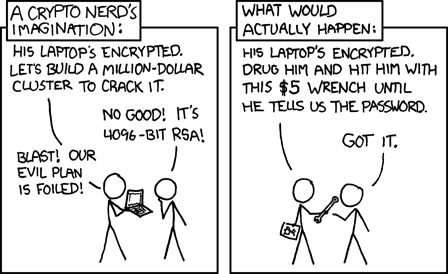
\includegraphics[width=0.5\textwidth]{images/xkcd-538}\\
\hfill (Source: xkcd 538)
\end{center}

\newtheorem{defn}{Definition}

\paragraph{Formalization.} Let's make the notion of ``expensive'' a bit more formal.
The idea is to force the use of the ``most memory possible'' for a given number of
operations. More memory implies more circuitry required to implement.

    \begin{defn}
      A \emph{memory-hard} algorithm on a Random Access Machine is an
      algorithm which uses $S(n)$ space and $T(n)$ operations, where
      $S(n) \in \Omega(T(n)^{1-\varepsilon})$.
    \end{defn}

Memory-hard algorithms are expensive to implement in either hardware or software.

Now, we want to move from particular algorithms to the underlying
functions (that is, we would like to quantify over all possible
algorithms). Intuitively, a \emph{sequential memory-hard function} is
one where (1) the fastest sequential algorithm is memory-hard; and (2)
it is impossible for a parallel algorithm to asymptotically achieve
lower cost.

\paragraph{Existence proof.} Of course anyone can define anything.
It's much better if the thing being defined actually exists. The
scrypt paper then goes on to exhibit ReMix, which is a concrete
example of a sequential memory hard function.

Finally, the paper concludes with an example of a more realistic
(cache-aware) model and a hard function in that context, BlockMix.

\paragraph{Rainbow Tables} So, the brute force approach is the simplest to describe but is computationally intensive, and if a sufficiently-well-designed cryptographic hash function is used it's really tough to actually crack a password. But maybe if we want to crack a password we don't have to always start from zero; maybe we could remember some previous computations so that we could use those answers later. If we calculated the hash of password ``12345'' and we knew what that looked like, if we encountered that hash in the future we could already jump immediately to the answer in our lookup table. This is the basic idea behind \textit{rainbow tables}.

There is a technical paper describing how rainbow tables work, but we'll instead use a much less cryptograhic-expert-level explanation~\cite{rainbowtables}. 

Part of the difficulty with this approach is that it isn't practical, or even really possible, to store the hashes for every possible plaintext (unless the plaintext is very small). So the rainbow table is a compromise between speed and space. The ``reduction'' function maps hashes to plaintext:

\begin{center}
	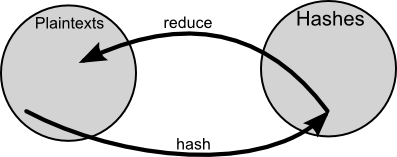
\includegraphics[width=0.4\textwidth]{images/rainbow-tables-reduce.png}\\
	Showing the reduce and hash functions~\cite{rainbowtables}.
\end{center}

This mapping function isn't the inverse of the hash function; it's just some sort of categorization. If the set of passwords to be cracked is, say, six digit numeric, then we compute the hash for a given input (``123456'') and we get some output (``d41d8cd98f00b204e9800998ecf8427e'') which is then reduced (mapped) to some other value (e.g., we'll take the first 6 numbers, 418980). We have another plaintext now, 418980. So we hash this new one, and reduce it, and so on and so on, until some end point ($n$ times, where you choose $n$). 

\begin{center}
	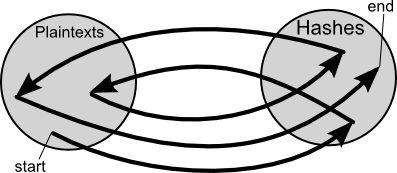
\includegraphics[width=0.4\textwidth]{images/rainbow-tables-chain.png}\\
	And now we have a chain~\cite{rainbowtables}.
\end{center}

We should do this to develop some number of chains. This is the sort of task you could do with a GPU, because they can do a reduction relatively efficiently. 

Once we have those developed for a specific input set and hash function, they can be re-used forever. You do not even need to make them yourself anymore (if you don't want) because you can download them on the internet... they are not hard to find. They are large, yes, but in the 25 - 900 GB range, which is large  but not ridiculous. I mean, Fallout 76 had a day one patch of 52 GB, and it was a disaster of a game.

Alright, so, you've got them (or made them), but how do we use rainbow tables? Well, for a given hash with an unknown plaintext~\cite{rainbowtables}:
\begin{enumerate}
	\item Look for the hash in the list of final hashes; if there, break out of the loop
	\item If it's not there, reduce the hash into another plaintext and hash the new plaintext
	\item Go back to step 1
	\item If the hash matches a final hash, the chain with the match contains the original hash
	\item Having identified the correct chain, we can start at the beginning of the chain with the starting plaintext and hash, check to see if we are successful (if so, we are done); if not, reduce and try the next plaintext. 
\end{enumerate} 

Like generation, checking the tables for a hit can also be done efficiently by the GPU. Some numbers from \url{http://www.cryptohaze.com/gpurainbowcracker.php.html}: 
\begin{itemize}
	\item Table generation on a GTX295 core for MD5 proceeds at around 430M links/sec.
	\item Cracking a password 'K\#n\&r4Z': real: 1m51.962s, user: 1m4.740s. sys: 0m15.320s
\end{itemize}

Yikes. There is obviously a little bit more complexity to how the rainbow tables work (such as dealing with collisions and loops), but it is clear just how devastatingly effective GPU computations are on breaking passwords.

\section*{The World is Not Enough}
GPUs are great at this, but there are some problems where even the GPU isn't quite the right choice. You have probably guessed it; we're going to talk about Bitcoin. Let's get it out there: I don't think you should mine Bitcoin. This tweet sums up how I would explain Bitcoin to my parents: \url{https://twitter.com/theophite/status/1030225104234373121?lang=en}... and in any case it's pretty uneconomic to mine it and it's terrible for the environment. At the time of writing, the Bitcoin network's carbon footprint is comparable to that of the entire country of Denmark and it uses electricity comparable to the entire power consumption of the country of Austria (source, and for updated figures, see: \url{https://digiconomist.net/bitcoin-energy-consumption}). Alright, enough of that: if you want to know more about why you shouldn't mine Bitcoin, talk to me after class. 

Our guide in this section is~\cite{bitcoin}, a paper that roughly overviews the history of Bitcoin, how it works, and the trend of mining rigs. 

Anyway---Bitcoin is ``mined'' by doing hash computations, specifically SHA-256. In the beginning, CPUs could be used to mine Bitcoin by performing the calculations. The difficulty of completing the next unit of work increases periodically, so it did not take long for CPU to be inefficient for this purpose. GPUs were the logical step but the quest for more is always ongoing and what do people do when GPU is exhausted?

That's right---they start looking at hardware. Specifically, custom hardware. This works well because the calculations needed are just cryptographic hashing and nothing else. So it's possible to design a system that is optimized to do the few operations in the hash computation (and, xor, rotate, add [modulo], or, right shift) which always happen in a specific order. There's no need for a general purpose CPU or GPU with lots of unnecessary functionality, which just wastes power...

 The first hardware miners were built using FPGAs, but they were quickly replaced by ASIC miners. ASIC miners are much more efficient, both in terms of hashes computed per second but also in terms of power consumption. And the more of these that go online, the harder the computation is and the difficulty of mining Bitcoin (in terms of time) increases. These advances make it basically impossible to mine with the hardware you already have.

So now we've uncovered why you shouldn't mine Bitcoin. If you want to do so in a cost-effective manner (otherwise what's the point), you have to spend money on a mining rig of some sort (which is a significant investment), and pay for the power consumption of it (which is also not zero), and some maintenance is required. And because the difficulty is high and new technology is constantly being released to mine more efficiently, it is quite likely that before long your mining setup costs more to run than is earned in Bitcoin. At which point: don't bother.

This isn't a hardware course so we're not going to invest a lot of time in talking about how one might cleverly design hardware. There are other courses for that, but it's the logical extension of using the GPU, so I thought it might be worth a mention.










\chapter*{25 --- Profiling: Observing Operations}

\addcontentsline{toc}{chapter}{25 --- Profiling: Observing Operations}

\section*{Observations Precede Conclusions}

Think back to the beginning of the course when we did a quiz on what operations are fast and what operations are not. The important takeaway was not that we needed to focus on how to micro-optimize this abstraction or that hash function, but that our intuition about what is fast and what is slow is often wrong. Not just at a macro level, but at a micro level. You may be able to narrow down that this computation of $x$ is slow, but if you examine it carefully\ldots what parts of it are slow?

If you don't use tools, then you end up guessing. You just make some assumptions about what you think is likely to be slow and try to change it. You've probably heard the famous quotation before, but here it is in its full form:

\begin{quote}
\textit{Programmers waste enormous amounts of time thinking about, or worrying about, the speed of noncritical parts of their programs, and these attempts at efficiency actually have a strong negative impact when debugging and maintenance are considered. We should forget about small efficiencies, say about 97\% of the time: premature optimization is the root of all evil. Yet we should not pass up our opportunities in that critical 3\%.}
\end{quote}
	\hfill -- Donald Knuth

So going about this blindly is probably a waste of time. You might be fortunate and optimize a slow part, but we should really follow one of my favourite rules: ``don't guess, measure!'' So, to make your programs or systems fast, you need to find out what is currently slow and improve it (duh!). Up until now in the course it's mostly been about ``let's speed this up'', but we did not take much time to decide what we should speed up (though you maybe did this on an assignment\ldots?).

The general idea is, collect some data on what parts of the code are taking up the majority of the time. This can be broken down into looking at what functions get called, or how long functions take, or what's using memory\ldots

\paragraph{Why Observation?} We're talking here about the idea of observation of our program, which is a little bit more inclusive than just measuring things, because we may observe things that are hard or impossible to quantify. Observing the behaviour of the program will obviously be super helpful in terms of figuring out what -- if anything -- to change. We have several different ways of looking at the situation, including logs, counters, profiling, and traces. Differences between them, briefly~\cite{usd}:

\begin{itemize}
	\item \textbf{Counters} are, well, a stored count of the occurrences of something: how many times we had a cache miss, how many times we called \texttt{foo()}, how many times a user logged in...
	\item \textbf{Profiles} are higher-level overviews of what the program is doing, where time is going in aggregate, and how long certain operations take.
	\item \textbf{Traces} are recordings that show the sequence of events that the program is doing, so we can understand the runtime behaviour and how we got to the state we are in.
\end{itemize}

We'll return to profilers later, because it's a big topic, but for now we'll start with traces and counters.

\subsection*{Tracing: Logging}
We'll start with the idea of logging. It's an effective way of finding out what's going on in your program as it executes, and probably all of us have use print statements as a form of debugging, but also as a form of tracing. When we're running a small program, we don't always make the log messages very nice, but in a production system, logs typically have a timestamp, a message, and some attributes. The timestamp is helpful for organizing and searching the logs. 

In~\cite{usd} it's recommended that if there can be only one tool for observing your program's execution, it is logging. This is because logging can tell you things about how much work the software did in a time period, when things are busy, which transactions are slow, when the service is down, etc. This probably matches well with our intuition that printf debugging or tracing is a good first option to figure out what's going on.

Given that we want to log, we do have to consider how often to log, and what should be in the content of it. If we don't log the information, there may not be any good way to recover that information again. But we could also drown out useful information if we log too many (irrelevant) things. Logs typically have levels, like error, warning, info, debug... These can make it easier to spot just the information that is relevant.

A typical approach is to log an incoming request (input) and the outgoing response (output), and maybe some steps in between. We want to link the different things together (perhaps with attributes) so that we can see what happened. Here's a made-up example that doesn't show the time stamps or attributes:

\begin{verbatim}
Received request: update plan of company 12345 to ULTIMATE
Retrieving company 12345
Verifying eligibility for upgrade of company 12345 from BASIC to ULTIMATE
Company 12345 is not eligible for upgrade due to: unpaid invoices > 0
Returning response: update of company 12345 to ULTIMATE is DECLINED
\end{verbatim}

We can see the various steps of the process and quickly understand what happened, because the logs show us the request, the stages of handling the request, and the response. In this example I intentionally added a decision and logged the reason for the decision. That's preferable to making someone guess why the answer was no when looking at the logs.

Choosing the timestamps strategy is also interesting; the level of precision you need in the logging depends on the timescales of your execution. When running processes that take tens of seconds, you could probably be satisfied with down to the thousandth of a second; if things run super fast then we might need microsecond or nanosecond resolution~\cite{usd}. Time zones also matter, but I'm going to recommend using UTC because it doesn't have weird things like Daylight Savings Time where you can get a jump in the time forward or back. And back is worse because it means a certain minute appears to happen more than once (defeating our normal expectation of linear time). It also avoids issues where the California team thinks it's Monday and the Singapore team thinks it's Tuesday. UTC might be weird, though, if your application is running on a Mars Rover; at that point you might as well use Stardates (Captain's Log, Stardate 46119.1...).

As I already said, logging every request might be too noisy to actually find anything in the resulting data. The ability to search and sort helps, but it can still be going by too fast to realistically assess in real-time. Log aggregation services exist and they can help, especially when trying to do a retrospective.

Typically, adding any relevant attributes is very helpful to identify what has happened or to correlate knowledge. If we can see in the attributes that updates for plans of companies always take ten times longer if the company's address is in Portugal, that's actually a useful observation. We can take that information and put it in the bug ticket and ideally help the developer -- even if it's our future selves -- to find the issue and resolve it.

With that said: there's such a thing as too much detail in logging. Logs should always redact personally-identifiable information such as people's names, contact information, medical records, etc. Unless the logs are really kept in secure storage with appropriate access controls, they can be seen by people who shouldn't have that information. Why should, for example, a developer on the website team have access to the banking details of a customer? My opinion: they shouldn't. And it's not just my opinion, but also the opinion of people like the Privacy Commissioner of Canada, whom you probably do not want to anger.

One way that we get into the situation of over-logging is if it's difficult or impossible to use other tools on the program or to have (read-)access to the database. If someone is trying to debug the behaviour of the program it might seem sensible to log just about everything because it's frustrating to try to debug a problem with incomplete information. 

So we are aiming for a balance: include the relevant information that would let us spot patterns or correlate with other data sources, but not so much that the important information is lost or that PII is exposed.

There is a third way that a program logging too much, beyond drowning out key info or logging PII, and that's if the overhead of tracing is significant. Normally we're happy to accept some small slowdown in our program to have traceability, but let's try to put some numbers to tracing overhead. 

Some quick, off-the-cuff figures from~\cite{usd}:
\begin{itemize}
	\item If we ask the CPU trace tool to track every conditional branch taken, that would be about a $20\times$ slowdown. This amount of overhead would be acceptable if we're debugging the program on a development machine (own laptop or testing deployment), but certainly not in a production environment.
	\item If we ask for a timestamp at every function call and return in our program the slowdown is around $1.2-1.5\times$. This may (emphasis on may) be acceptable in a production environment if the task is not time-critical, but only temporarily while experimenting or observing.
	\item If we ask for a timestamp of every system call entry and exit (user-space to kernel transition and back), that might be much less than $1\%$ overhead. This would likely be acceptable in a production environment for all but the most time-critical of operations and could remain in place at all times.
\end{itemize}

That covers tracing the CPU. What about memory? If you've used Valgrind\footnote{So, we used to cover Valgrind in this course. That made sense when it was C and \CPP~but we used to discuss it in Rust too. While the Helgrind part might help you find lock acquisition issues, for the most part students found that there were too many false positives around memcheck and it was just causing students to stress about losing marks. So... away with it.} before, you know it. If you haven't, as I say to the ECE~252 students: The target program then runs under the ``supervision'' of the tool. This results in running dramatically slower than normal, but you get additional checks and monitoring of the program. Why? Valgrind checks every memory read and write for validity (is the variable initialized? Is it off the end of an array? All those fun things that we, fortunately, no longer think about in Rust), but also records information about where memory is allocated to help the programmer in tracking down the genesis of a memory leak. When execution of the program ends, Valgrind shows the stack trace of the path that led to the allocation that was leaked. That's pretty neat!

A disk trace tool would most likely have extremely tiny overhead because the speed of the disk as compared to the CPU is very slow. Something similar goes for the network; the latency is high and speed of the network are slow compared to what the CPU can do~\cite{usd}. 

Tracing also can play a role in identifying deadlocks and delays in threads caused by waiting for locks: simply log every lock and unlock. But we might really be only interested in the locks where there is contention, i.e., threads are sometimes or often failing to acquire the lock because it's held by another thread~\cite{usd}. After all, if our intention is to observe the behaviour of the program with the intention of improving performance, the part where a thread isn't getting what it wants immediately and must wait is much more interesting than the part where everything is fine and there are no delays.

\paragraph{Space, the Final Frontier.} Whatever trace strategy we choose, the trace itself takes up space. If we are producing a very large amount of data, it won't all fit in memory and has to go on disk. It's possible that the amount of data that we produce will fill up the disk very quickly, or arrive so fast that the disk cannot keep up. In~\cite{usd} there's a quick calculation that says a main memory system with 20 GB/s bandwidth and 64-byte cache lines that records up to 8 bytes of data per trace entry could result in producing data at a rate of 2.4 GB per second! That's a rather overwhelming amount of data -- even if you could write it all out to disk fast enough, it would fill up an 8 TB hard drive in just under an hour. Either we need to capture less data by recording fewer things or by recording for a shorter time. Just add this to the reasons why we need to be judicious about how much trace data to capture.

\subsection*{Aggregate Measures (Counters)}
Many profiling tools rely heavily on counters. Counters, as the name suggests, keep a count of events: interrupts, cache misses, data bytes written, calls to function \texttt{do\_magic()}. Keeping track of these numbers is relatively inexpensive (specially when compared to other approaches so counting every occurrence of an event is actually plausible. Counters are a form of aggregation, because we're summing the number of occurrences and at the end of the program we have a total number. The counter any any data derived from it certainly takes much less space than a trace.

The sum is the simplest kind, but other aggregate measures are exactly what they sound like: summaries of data. Calculating the average response time of a request is an aggregate measure: we've summed up the total time per request and divided it by the number of requests in the given period and hopefully the resulting value is a useful one. Asking the computer to calculate the summary is sensible, of course, because it's not realistic to ask a human to look at 50~000 requests and calculate their average time. Some obvious aggregate measures are things like: number of requests, requests broken down by type, average time to respond to a request, percentage of error responses...  

Whatever aggregate measures we use, they are useful only with context.  Suppose that after my pull request is merged, the average login time for a user is 0.75 seconds; is that a problem? Without a baseline to compare against, I'm not sure. If before my PR it was 0.5 seconds, I made performance much worse and that doesn't sound good; should I revert it and re-work it? Maybe, unless I am intentionally making login slower to make a brute-force password attack more expensive for an attacker. Context is key: the summary tells you some data, but not the reasons.

Another example: if I tell you that a request takes, on average, 1.27 seconds to get a response, is that good or bad? There's, again, no way to say anything about it without a point of reference. Are we being asked to approve or deny a transaction and there's a time limit of 1 second to give our answer (or else a default answer is assumed)? We're missing the target and that's a problem. If instead I said the time limit is 10 seconds, then we have plenty of room. Or do we?

Average time isn't quite enough to know if we're doing well when it comes to time limits. If the average time is 1.27 seconds it does not preclude the possibility that the maximum time is outside the 10 second time limit and that means for some percentage of requests, possibly a large percentage, we're not making the deadline. How hard of a deadline are we talking about? To address this we can look at maximum and 95th percentile kind of aggregate measures as well.

The other way that averages can be misleading is that they misrepresent the bursty nature of the data. If your service receives, on average, 7 requests per second, does that mean it looks like the first, second, or third row below (all from~\cite{usd})?

\begin{center}
	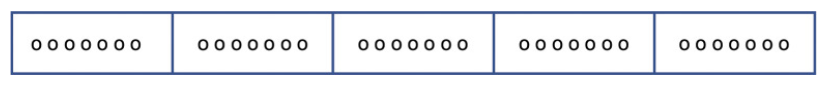
\includegraphics{images/burst1}\\
	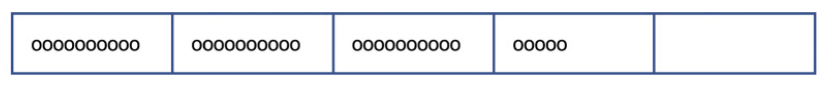
\includegraphics{images/burst2}\\
	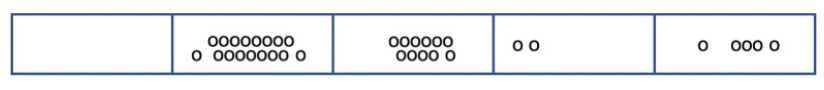
\includegraphics{images/burst3}\\
\end{center}

While the first scenario is really nice and very predictable, is that realistic? Later on in the course we'll talk more about queueing theory and we'll learn that random arrivals and what it means for things to arrive.

When we choose to aggregate our data in some way, we must make a decision about the period of time in question. If our program is going to, say encode a video, the period of time is probably the whole execution time of the task: it took 3h 21 minutes to encode the video and that results in a processing rate of 210.9 frames per second. For services that run indefinitely or when we're impatient, we might want to look at a shorter period of time and consider that. But if we choose the wrong period we'll miss important things: if we look at purchases per hour, if we look at Sunday night that might be misleading as compared to Monday at noon.

\paragraph{Look at the pretty pictures.} 
Often, we want to not just see the raw data, but also the trend in the data; choosing the right visualization is really helpful. Digital speedometers in cars are more accurate than a sweep one in terms of showing you the speed of your vehicle, but the sweeping analog speedometer makes it easier for a person to understand the acceleration (rate of change of that speed). Representing changes in data over time in a graph makes it easier to identify trends or alarming things, and as a bonus, managers and non-technical people love them and love to rely on them. 

Consider just a simple example of the CPU usage graph from my laptop when I compile and run the nbody-parallel code; the blue represents user-space execution and red represents kernel execution:

\begin{center}
	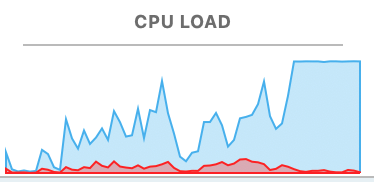
\includegraphics[width=0.3\textwidth]{images/cpu-load.png}
\end{center}

It is obvious in this picture at what point the simulation starts running for real. If we see this and we can identify an operation that starts around the time the CPU is maxed out, we have found something useful.

\paragraph{Dashboards.} If we put together enough pretty pictures, we get a... dashboard! Dashboards are (ideally) more than just pretty pictures of LINE GOES UP. It is instead intended to be a collection of useful graphs (time trends, histograms, etc) that present an easily-digestible summary of the situation. Good dashboards make it clear what's happening and what things need attention. Of course, dashboards tend to make more sense when we have many things to measure; not so much if we're just trying to optimize one specific thing.

\subsection*{Drill-down}
All of this introduction to profiling has really been focused around the higher level ideas for identifying what's happening and what operations, if any, are slow (or slower than expected). Once we know that, for example, importing CSV files with tax rates is slow, we can start to use some profiling tools to identify what is slow inside that functionality.  In the next topic, we'll start by narrowing down what area is the bottleneck. 










\chapter*{26 --- Profiling and Scalability}

\addcontentsline{toc}{chapter}{26 --- Profiling and Scalability}

\section*{Profiling and Scalability}

We've had a long look at the subject of observation -- identifying areas in the execution of our program that are a potential issue. Most of our upcoming discussion will be around the idea of CPU profiling, which is to say, examining where CPU time is going. That's generally predicated on the idea that CPU time is limiting factor. But maybe it isn't, and before we go about focusing on how to improve this aspect, let's check that assumption and consider what else it could be.

While we're discussing this, we will also take some time to relate performance to scalability. Very early on in the course we mentioned the idea that what we want in scalability is to take our software from 1 user to 100 to 10 million. To scale up, we probably need to do some profiling to find out what's slow and make a decision about what to change. It's also useful in terms of making an estimate of our maximum number of users or transactions could be. That's not a hypothetical scenario either; I [JZ] was asked by a C-Level (company executive) whether a particular system could handle 10$\times$ as many users -- and that answer had to be supported with some numbers.

With that said, if you identify a problem in a production system and we want to experiment on it with a dev machine, or if we have an application developed and we want to estimate what its performance and limiting factors would be, there are a few things we need to worry about.  So we should respect the following principles, as outlined in~\cite{swps}.

\paragraph{Hardware Principle.} 
Scalability testing is very different from  QA testing (you test your code, right?) in that you will do development and QA on your local computer and all you really care about is whether the program produces the correct output ``fast enough''. That's fine, but it's no way to test if it scales. If you actually want to test for scalability and real world performance, you should be doing it on the machines that are going to run the program in the live/production environment. Why? Well, low-end systems have very different limiting factors. You might be limited by the 16GB of RAM in your laptop and that would go away in the 64GB of RAM server you're using. So you might spend a great deal of time worrying about RAM usage when it turns out it doesn't matter.

\paragraph{Reality Principle.}
It would be a good idea to use a ``real'' workload, as much as one can possibly simulate. Legal reasons might prevent you from using actual customer data, but you should be trying to use the best approximation of it that you have. 

If you only generate some test data, it might not be representative of the actual data: you might say 1\% of your customers are on the annual subscription but if it's really 10\% that might make a difference in how long it takes to run an analysis. On the other hand, your test data might be much larger than in production because your tests create (and don't delete) entities in the test system database every time you run.

This isn't theoretical: I [JZ] have been the incident responder on an incident where an app doesn't start up because the database migration takes too long and gets killed. This issue wasn't caught in the test environment because the size of data there was much smaller than the live database. So of course the migration was finished well under the time limit during testing... and failed when going live. Oops.

Related to that, user behaviour is hard to simulate, too. If you are making threads that pretend to be users to simulate concurrent usage of the system, the scripts those threads run may not accurately represent the way the users really behave.  Your test example scenario may assume that company managers want to run the report once a month... your users might run them every hour. That one really happened to me [JZ] as well. The manager was using the report to keep an eye on what his team members were doing all day!

\paragraph{Volume Principle.}
``More is the new more.'' It's okay to use lighter workloads for regression testing and things like that, but if you actually want to see how your system performs under pressure, you actually need to put it under pressure! You can simulate pressure by limiting RAM or running something very CPU-intensive concurrently, but it's not quite the same as having an actually-high workload. 

Why not? The issue isn't so much the test as it is what you're not seeing. If I want to test the app on my laptop under CPU pressure I can just run the app while I repeatedly convert a lecture video just to consume CPU cycles. That does have the effect of limited CPU time available and we can see how the app performs when CPU time is maxed out. But that's not the same as what happens if you have 500 users concurrently, because you might not get to full CPU usage with 500 users due to other reasons, such as lock contention. 

These tests, incidentally, are of great interest to the customers and C-Levels, who would like to know that you can deliver promised levels of performance or throughput, or what the current maximum is.

\paragraph{Reproducibility and Regression Testing.}
Your results will need to be reproducible. Remember that good programming practice says that tests should be run, and re-run to make sure it all works. The same is true in your performance tests. Just as we don't want to see old bugs cropping up again, old (solved) performance issues are not nice to see either. Or a new change that slows the whole program down is not a success either. So please, have regression testing and performance regression testing. Real-life example: \url{https://arewefastyet.com} tracks regressions/improvements in Firefox performance.

\section*{Characterizing Performance \& Scalability Problems}

\begin{quote}
\textit{It is a capital mistake to theorize before one has data. Insensibly one begins to twist facts to suit theories, instead of theories to suit facts.}
\end{quote}
\hfill - Sherlock Holmes (\textit{A Scandal in Bohemia}; Sir Arthur Conan Doyle)

Keeping the wisdom of Mr. Holmes in mind, we need to collect evidence before reaching conclusions. At a high level we probably have five potential culprits to start with:
\begin{enumerate}
	\item CPU
	\item Memory
	\item Disk
	\item Network
	\item Locks
\end{enumerate}

These are, obviously, more categories than specific causes, but they are starting points for further investigation. They are listed in some numerical order, but there is no reason why one would have to investigate them in the order defined there.

\paragraph{CPU.} CPU is probably the easiest of these to diagnose. Something like \texttt{top} or Task Manager will tell you pretty quickly if the CPU is busy. You can look at the \%CPU columns and see where all your CPU is going. Still, that tells you about right now; what about the long term average? Checking with my machine ``Loki'', that used to donate its free CPU cycles to world community grid (I'm singlehandedly saving the world, you see.):

\begin{verbatim}
top - 07:28:19 up 151 days, 23:38,  8 users,  load average: 0.87, 0.92, 0.91
\end{verbatim}

Those last three numbers are the one, five, and fifteen minute averages of CPU load, respectively. Lower numbers mean less CPU usage and a less busy machine. A small guide on how to interpret this, from~\cite{scout}.

Picture a single core of a CPU as a lane of traffic. You are a bridge operator and so you need to monitor how many cars are waiting to cross that bridge. If no cars are waiting, traffic is good and drivers are happy. If there is a backup of cars, then there will be delays. Our numbering scheme corresponds to this:

\begin{enumerate}
	\item 0.00 means no traffic (and in fact anything between 0.00 and 0.99) means we're under capacity and there will be no delay.
	\item 1.00 means we are exactly at capacity. Everything is okay, but if one more car shows up, there will be a delay.
	\item Anything above 1.00 means there's a backup (delay). If we have 2.00 load, then the bridge is full and there's an equal number of cars waiting to get on the bridge. 
\end{enumerate}

Or, visually, also from~\cite{scout}:

\begin{center}
	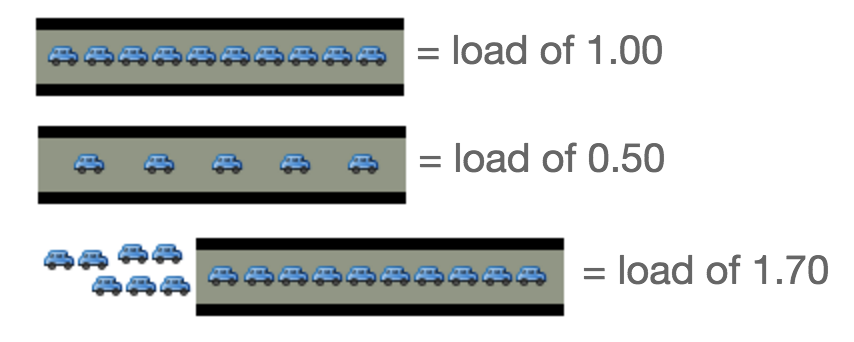
\includegraphics[width=0.55\textwidth]{images/car-analogy.png}
\end{center}

Being at or above 1.00 isn't necessarily bad, but you should be concerned if there is consistent load of 1.00 or above. And if you are below 1.00 but getting close to it, you know how much room you have to scale things up -- if load is 0.4 you can increase handily. If load is 0.9 you're pushing the limit already. If load is above 0.70 then it's probably time to investigate. If it's at 1.00 consistently we have a serious problem. If it's up to 5.00 then this is a red alert situation.

Now this is for a single CPU -- if you have a load of 3.00 and a quad core CPU, this is okay. You have, in the traffic analogy, four lanes of traffic, of which 3 are being used to capacity. So we have a fourth lane free and it's as if we're at 75\% utilization on a single CPU.


\paragraph{Memory and Disk.} Next on the list is memory. One way to tell if memory is the limiting factor is actually to look at disk utilization. If there is not enough RAM in the box, there will be swapping and then performance goes out the window and scalability goes with. That is of course, the worst case. You can ask via \texttt{top} about how much swap is being used, but that's probably not the interesting value. 

\begin{verbatim}
KiB Mem:   8167736 total,  6754408 used,  1413328 free,   172256 buffers
KiB Swap:  8378364 total,  1313972 used,  7064392 free.  2084336 cached Mem
\end{verbatim}

This can be misleading though, because memory being ``full'' does not necessarily mean anything bad. It means the resource is being used to its maximum potential, yes, but there is no benefit to keeping a block of memory open for no reason. Things will move into and out of memory as they need to, and nobody hands out medals to indicate that you did an awesome job of keeping free memory. It's not like going under budget in your department for the year.  Also, memory is not like the CPU; if there's nothing for the CPU to do, it will just idle (or go to a low power state, which is nice for saving the planet). But memory won't ``forget'' data if it doesn't happen to be needed right now - data will hang around in memory until there is a reason to move or change it. So freaking out about memory appearing as full is kind of like getting all in a knot about how ``System Idle Process'' is hammering the CPU\footnote{Yes, a tech journalist named John Dvorak really wrote an article about this, and I will never, ever forgive him for it.}.

You can also ask about page faults, with the command \texttt{ps -eo min\_flt,maj\_flt,cmd} which will give you the major page faults (had to fetch from disk) and minor page faults (had to copy a page from another process). The output of this is too big even for the notes, but try it yourself (or I might be able to do a demo of it in class). But this is lifetime and you could have a trillion page faults at the beginning of your program and then after that everything is fine. What you really want is to ask Linux for a report on swapping:

\begin{verbatim}
jz@Loki:~$ vmstat 5
procs -----------memory---------- ---swap-- -----io---- -system-- ------cpu-----
 r  b   swpd   free   buff  cache   si   so    bi    bo   in   cs us sy id wa st
 1  0 1313972 1414600 172232 2084296    0    0     3    39    1    1 27  1 72  0  0
 0  0 1313972 1414476 172232 2084296    0    0     0    21  359  735 19  0 80  0  0
 0  0 1313972 1414656 172236 2084228    0    0     0   102  388  758 22  0 78  0  0
 4  0 1313972 1414592 172240 2084292    0    0     0    16  501  847 33  0 67  0  0
 0  0 1313972 1412028 172240 2084296    0    0     0     0  459  814 29  0 71  0  0
\end{verbatim}

In particular, the columns ``si'' (swap in) and ``so'' (swap out) are the ones to pay attention to. In the above example, they are all zero. That is excellent and tends to indicate that we are not swapping to disk and that's not the performance limiting factor. Sometimes we don't get that situation. A little bit of swapping may be inevitable, but if we have lots of swapping, we have a very big problem. Here's a not-so-nice example, from~\cite{vmstat}:

\begin{verbatim}
  procs                      memory    swap          io     system cpu
r  b  w   swpd   free  buff cache  si  so   bi   bo   in    cs us  sy  id
. . .
1  0  0  13344   1444  1308 19692   0 168  129   42 1505   713 20  11  69
1  0  0  13856   1640  1308 18524  64 516  379  129 4341   646 24  34  42
3  0  0  13856   1084  1308 18316  56  64   14    0  320  1022 84   9   8
\end{verbatim}

If we're not doing significant swapping, then memory isn't holding us back, so we can conclude it is not the limiting factor in scaling the application up. On to disk.

Looking at disk might seem slightly redundant if memory is not the limiting factor. After all, if the data were in memory it would be unnecessary to go to disk in the first place. Still, sometimes we can take a look at the disk and see if that is our bottleneck.

{\scriptsize
\begin{verbatim}
jz@Loki:~$ iostat -dx /dev/sda 5 
Linux 3.13.0-24-generic (Loki) 	16-02-13 	_x86_64_	(4 CPU)

Device:         rrqm/s   wrqm/s     r/s     w/s    rkB/s    wkB/s avgrq-sz avgqu-sz   await r_await w_await  svctm  %util
sda               0.24     2.78    0.45    2.40    11.60   154.98   116.91     0.17   61.07   11.57   70.27   4.70   1.34
\end{verbatim}
}

It's that last column, \%util that tells us what we want to know. The device bandwidth here is barely being used at all. If you saw it up at 100\% then you would know that the disk was being maxed out and that would be a pretty obvious indicator that it is the limiting factor. This does not tell you much about what is using the CPU, of course, and you can look at what processes are using the I/O subsystems with \texttt{iotop} which requires root privileges\footnote{https://xkcd.com/149/}.

\paragraph{Network.} That leaves us with networks. We can ask about the network with \texttt{nload}: which gives the current, average, min, max, and total values. And you get a nice little graph if there is anything to see. It's not so much fun if nothing is happening. But you'll get the summary, at least:

\begin{verbatim}
Curr: 3.32 kBit/s
Avg: 2.95 kBit/s
Min: 1.02 kBit/s
Max: 12.60 kBit/s
Ttl: 39.76 GByte                                                                                       \end{verbatim}

\paragraph{Locks.}
The last possibility we'll consider is that your code is slow because we're waiting for locks, either frequently or for lengthy periods of time. We've already discussed appropriate use of locks, so we won't repeat that. The discussion here is about how to tell if there is a locking problem in the first place.

We'll exclude the discussion of detecting deadlock, because we'll say that deadlock is a correctness problem more than a performance problem. In any case, a previous course (ECE 252, SE 350, MTE 241) very likely covered the idea of deadlock and how to avoid it. The Helgrind tool (Valgrind suite) is a good way to identify things like lock ordering problems that cause a deadlock. Onwards then. 

Unexpectedly low CPU usage, that's not explained by I/O-waits, may be a good indicator of lock contention. If that's the case, when CPU usage is low we would see many threads are blocked. 

Unlike some of the other things we've discussed, there's no magical \texttt{locktrace} tool that would tell us about critical section locks, and the POSIX pthread library does not have any locks tracing in its specification~\cite{usd}. One possibility is to introduce some logging or tracing ourselves, e.g., recording in the log that we want to enter a critical section $A$ and then another entry once we're in it and a third entry when we leave $A$. That's not great, but it is something! 

I did some reading about \texttt{perf lock} but the problem is, as above, that it doesn't really find user-space lock contention. You can ask tools to tell you about thread switches but that's not quite the same. Other commercial tools like the Intel VTune claim that they can find these sorts of problems. But those cost money and may be CPU-vendor-specific.


\subsection*{But it's probably CPU...}
Most profiling tools, and most of our discussion, will be about CPU profiling. It's the most likely problem we'll face and something that we are hopefully able to do something about. 









\chapter*{27 --- Program Profiling and POGO}

\addcontentsline{toc}{chapter}{27 --- Program Profiling and POGO}

\section*{Profiling}
We've spent some time talking about observing programs at a higher level, but now we should consider zooming in a little bit to using specific profiling tools to figure out where CPU time is going and how to make use of that.

I've used the logging-only approach myself to figure out what blocks of a single large function are taking a long time (such as a time when I found out that updating exchange rates was slow.). But this approach is not necessarily a good one.  It's an example of ``invasive'' profiling---we are going in and changing the source code of the program in question---to add (slow!) instrumentation (log/debug statements). Plus we have to do a lot of manual accounting. Assuming your program is fast and goes through functions quickly and often, trying to put the pieces together manually is hopeless. It worked in that one example because the single function itself was running in the half-hour range and I could see that the save operation was taking twelve minutes. Not kidding.

I also mentioned earlier that I used the profiling tool for CUDA to find out what was wrong with my N-Body program. I ran the command \texttt{nvprof target/release/nbody-cuda}, and in addition to the regular program output I got the following, which showed that the time was going to the kernel and I wasn't losing a lot in overhead:

{\scriptsize
\begin{verbatim}
==20734== Profiling application: target/release/nbody-cuda
==20734== Profiling result:
            Type  Time(%)      Time     Calls       Avg       Min       Max  Name
 GPU activities:  100.00%  10.7599s         1  10.7599s  10.7599s  10.7599s  calculate_forces
                    0.00%  234.72us         2  117.36us  100.80us  133.92us  [CUDA memcpy HtoD]
                    0.00%  94.241us         1  94.241us  94.241us  94.241us  [CUDA memcpy DtoH]
      API calls:   97.48%  10.7599s         1  10.7599s  10.7599s  10.7599s  cuStreamSynchronize
                    1.92%  211.87ms         1  211.87ms  211.87ms  211.87ms  cuCtxCreate
                    0.54%  59.648ms         1  59.648ms  59.648ms  59.648ms  cuCtxDestroy
                    0.04%  4.8704ms         1  4.8704ms  4.8704ms  4.8704ms  cuModuleLoadData
                    0.00%  404.72us         2  202.36us  194.51us  210.21us  cuMemAlloc
                    0.00%  400.58us         2  200.29us  158.08us  242.50us  cuMemcpyHtoD
                    0.00%  299.30us         2  149.65us  121.42us  177.88us  cuMemFree
                    0.00%  243.86us         1  243.86us  243.86us  243.86us  cuMemcpyDtoH
                    0.00%  85.000us         1  85.000us  85.000us  85.000us  cuModuleUnload
                    0.00%  41.356us         1  41.356us  41.356us  41.356us  cuLaunchKernel
                    0.00%  18.483us         1  18.483us  18.483us  18.483us  cuStreamCreateWithPriority
                    0.00%  9.0780us         1  9.0780us  9.0780us  9.0780us  cuStreamDestroy
                    0.00%  2.2080us         2  1.1040us     215ns  1.9930us  cuDeviceGetCount
                    0.00%  1.4600us         1  1.4600us  1.4600us  1.4600us  cuModuleGetFunction
                    0.00%  1.1810us         2     590ns     214ns     967ns  cuDeviceGet
                    0.00%     929ns         3     309ns     230ns     469ns  cuDeviceGetAttribute
\end{verbatim}
}

Oh, and for comparison, here's the one where I make much better use of the GPU's capabilities (with better grid and block settings):

{\scriptsize
\begin{verbatim}
=22619== Profiling result:
            Type  Time(%)      Time     Calls       Avg       Min       Max  Name
 GPU activities:   99.92%  417.53ms         1  417.53ms  417.53ms  417.53ms  calculate_forces
                    0.06%  236.03us         2  118.02us  101.44us  134.59us  [CUDA memcpy HtoD]
                    0.02%  93.057us         1  93.057us  93.057us  93.057us  [CUDA memcpy DtoH]
      API calls:   52.09%  417.54ms         1  417.54ms  417.54ms  417.54ms  cuStreamSynchronize
                   26.70%  214.00ms         1  214.00ms  214.00ms  214.00ms  cuCtxCreate
                   13.63%  109.26ms         1  109.26ms  109.26ms  109.26ms  cuModuleLoadData
                    7.42%  59.502ms         1  59.502ms  59.502ms  59.502ms  cuCtxDestroy
                    0.05%  364.08us         2  182.04us  147.65us  216.42us  cuMemcpyHtoD
                    0.04%  306.48us         2  153.24us  134.10us  172.37us  cuMemAlloc
                    0.04%  285.73us         2  142.86us  122.90us  162.83us  cuMemFree
                    0.03%  246.37us         1  246.37us  246.37us  246.37us  cuMemcpyDtoH
                    0.01%  61.916us         1  61.916us  61.916us  61.916us  cuModuleUnload
                    0.00%  26.218us         1  26.218us  26.218us  26.218us  cuLaunchKernel
                    0.00%  15.902us         1  15.902us  15.902us  15.902us  cuStreamCreateWithPriority
                    0.00%  9.0760us         1  9.0760us  9.0760us  9.0760us  cuStreamDestroy
                    0.00%  1.6720us         2     836ns     203ns  1.4690us  cuDeviceGetCount
                    0.00%  1.0950us         1  1.0950us  1.0950us  1.0950us  cuModuleGetFunction
                    0.00%     888ns         3     296ns     222ns     442ns  cuDeviceGetAttribute
                    0.00%     712ns         2     356ns     212ns     500ns  cuDeviceGet
\end{verbatim}
}


Nicholas Nethercote wrote the ``counts'' tool\footnote{\url{https://github.com/nnethercote/counts}} to process ad-hoc debug output and shows an example of using it to profile the size of heap allocations in Firefox. In the example in the README, he reports that while most allocations are small, most memory is allocated as part of a large allocation. He provides a number of other examples where ad-hoc profiling is useful: how often are certain paths executed? how many times does a loop iterate? how many elements are in a hash table at a given location? And more! It's hard to write a general-purpose tool for these ad-hoc queries.

(Also like debugging, if you get to be a wizard you can maybe do it by code inspection, but that technique of speculative execution inside your head is a lot harder to apply to performance problems than it is to debugging. Trained professionals like Nicholas Nethercote use profilers, so you can too.)

So we should all agree, we want to use tools and do this in a methodical way.

Now that we agree on that, let's think about how profiling tools work\:

\begin{itemize}[noitemsep]
\item sampling-based (traditional): every so often (e.g. 100ms for gprof), stop the system and ask it what it's doing (query the system state); or,
\item instrumentation-based, or probe-based/predicate-based
  (sometimes, too expensive): query system state under certain
  conditions; like conditional breakpoints.
\end{itemize}
We'll talk about both per-process profiling and system-wide profiling. You can read more about profiling in Chapter 5 (Profiling) of The Rust Performance Book~\cite{nethercote20:_rust_perfor_book}; it discusses heap profiling in much more detail than we do (or don't,
more accurately).

If you need your system to run fast, you need to start profiling
and benchmarking as soon as you can run the system. Benefits:
\begin{itemize}[noitemsep]
\item establishes a baseline performance for the system;
\item allows you to measure impacts of changes and further system development;
\item allows you to re-design the system before it's too late;
\item avoids the need for ``perf spray'' to make the system faster, since
that spray is often made of ``unobtainium''\footnote{\url{http://en.wikipedia.org/wiki/Unobtainium}}.
\end{itemize}

\paragraph{Tips for Leveraging Profiling.}
When writing large software projects:
  \begin{itemize}[noitemsep]
    \item First, write clear and concise code. Don't do any premature optimizations---focus on correctness. Still, there are choices you can make that support performance at this stage, like using an efficient search or sort algorithm, if you know it's better and won't take additional effort.
    \item Once it's working, profile to get a baseline of your performance: it allows you to easily track any performance changes and to re-design your program before it's too late.
  \end{itemize}
Focus your optimization efforts on the code that matters.

Look for abnormalities; in particular, you're looking for
deviations from the following rules:
\begin{itemize}[noitemsep]
\item time is spent in the right part of the system/program;
\item time is not spent in error-handling, noncritical code, or exceptional cases; and
\item time is not unnecessarily spent in the operating system.
\end{itemize}
For instance, ``why is {\tt ps} taking up all my cycles?'';
see page 34 of ~\cite{300ps}.

\paragraph{Development vs. production.}
You can always profile your systems in development, but that might not
help with complexities in production. (You want separate dev and
production systems, of course!) We'll talk a bit about DTrace, which
is one way of profiling a production system. The constraints on profiling 
production systems are that the profiling must not affect the system's
performance or reliability.

\section*{Userspace per-process profiling}
Sometimes---or, in this course, often---you can get away with
investigating just one process and get useful results about that
process's behaviour.  We'll first talk about {\tt perf}, the profiler 
recommended for use with Rust. This is Linux-specific, though.

The \texttt{perf} tool is an interface to the Linux kernel's built-in
sample-based profiling using CPU counters. It works per-process, per-CPU, or system-wide. It can report the cost of each line of code.

Webpage: \url{https://perf.wiki.kernel.org/index.php/Tutorial}

\noindent
Here's a usage example on some old assignment code from a previous offering of the course:
\begin{lstlisting}[basicstyle=\scriptsize]
[plam@lynch nm-morph]$ perf stat ./test_harness

 Performance counter stats for './test_harness':

       6562.501429 task-clock                #    0.997 CPUs utilized          
               666 context-switches          #    0.101 K/sec                  
                 0 cpu-migrations            #    0.000 K/sec                  
             3,791 page-faults               #    0.578 K/sec                  
    24,874,267,078 cycles                    #    3.790 GHz                     [83.32%]
    12,565,457,337 stalled-cycles-frontend   #   50.52% frontend cycles idle    [83.31%]
     5,874,853,028 stalled-cycles-backend    #   23.62% backend  cycles idle    [66.63%]
    33,787,408,650 instructions              #    1.36  insns per cycle        
                                             #    0.37  stalled cycles per insn [83.32%]
     5,271,501,213 branches                  #  803.276 M/sec                   [83.38%]
       155,568,356 branch-misses             #    2.95% of all branches         [83.36%]

       6.580225847 seconds time elapsed
\end{lstlisting} %$

Right, let's get started. We're going to use the blog post~\cite{rustflamegraph} as a guide; that source tells a more complete story of an example of using the profiler to optimize, but for now we are just interested in the steps.

The first thing to do is to compile with debugging info, go to your \texttt{Cargo.toml} file and add:
\begin{verbatim}
[profile.release]
debug = true
\end{verbatim}

This means that \texttt{cargo build --release} will now compile the version with debug info (you can tell because it will say \texttt{Finished release [optimized + debuginfo] target(s) in 0.55s}; without this, we wouldn't get the part that says debug info so we can tell if it's correct. And we want it to be the release version that we're instrumenting, because we want the compiler optimizations to be applied. Without those, we might be trying to optimize things where the compiler would do it for us anyway.

The basic plan is to run the program using \texttt{perf record}, which will sample the execution of the program to produce a data set. Then there are three ways we can look at the code: \texttt{perf report}, \texttt{perf annotate}, and a flamegraph. We'll look at all of those, but in a live demo.


\paragraph{CLion.} While we've seen how to use \texttt{perf}, it's not the only way. During development of some of the code exercises, I used the CLion built-in profiler for this purpose. It generates a flamegraph for you too, and I'll show that for how to create the flamegraph as well.

\section*{Profiler Guided Optimization (POGO)}

In 2015 we were fortunate enough to have a guest lecture from someone at Microsoft actually in the room to give the guest lecture on the subject of Profile Guided Optimization (or POGO). In subsequent years, I was not able to convince him to fly in just for the lecture. Anyway, let's talk about the subject, which is by no means restricted to Rust.

The compiler does static analysis of the code you've written and makes its best guesses about what is likely to happen. The canonical example for this is branch prediction: there is an if-else block and the compiler will then guess about which is more likely and optimize for that version. Consider three examples, originally from~\cite{pogo} but replaced with some Rust equivalents:

\begin{lstlisting}[language=Rust]
fn which_branch(a: i32, b: i32) {
    if a < b {
        println!("Case one.");
    } else {
        println!("Case two.");
    }
}
\end{lstlisting}

Just looking at this, which is more likely, \texttt{a < b} or \texttt{a >= b}? Assuming there's no other information in the system the compiler can believe that one is more likely than the other, or having no real information, use a fallback rule. This works, but what if we are wrong? Suppose the compiler decides it is likely that \texttt{a} is the larger value and it optimizes for that version. However, it is only the case 5\% of the time, so most of the time the prediction is wrong. That's unpleasant. But the only way to know is to actually run the program.

\begin{multicols}{2}
\begin{lstlisting}[language=Rust]
trait Polite {
    fn greet(&self) -> String;
}

struct Kenobi {
    /* Stuff */
}
impl Polite for Kenobi {
    fn greet(&self) -> String {
        return String::from("Hello there!");
    }
}
\end{lstlisting}
\columnbreak
\begin{lstlisting}[language=Rust]
struct Grievous {
    /* Things */
}
impl Polite for Grievous {
    fn greet(&self) -> String {
        return String::from("General Kenobi.");
    }
}

fn devirtualization(thing: &Polite) {
    println!("{}", thing.greet());
}

\end{lstlisting}
\end{multicols}



There are similar questions raised for the other two examples. What is the ``normal'' type for some reference \texttt{thing}? It could be of either type \texttt{Kenobi} or \texttt{Grievous}. If we do not know, the compiler cannot do devirtualization (replace this virtual call with a real one). If there was exactly one type that implements the \texttt{Polite} trait we wouldn't have to guess. But are we much more likely to see \texttt{Kenobi} than \texttt{Grievous}?

\begin{lstlisting}[language=Rust]
fn match_thing(x: i32) -> i32 {
    match x {
        0..10 => 1,
        11..100 => 2,
        _ => 0
    }
}
\end{lstlisting}

 Same thing with \texttt{x}: what is its typical value? If we know that, it is our prediction. Actually, in a match block with many options, could we rank them in descending order of likelihood?

There exists a solution to this, and it is that we can give hints to the compiler, but that's a manual process. Automation is a good thing and this lecture is about that. These sorts of things already exist for Java! The Java HotSpot virtual machine will update its predictions on the fly. There are some initial predictions and if they turn out to be wrong, the Just In Time compiler will replace it with the other version. That's neat! I don't know for certain but I suspect the .NET runtime will do the same for something like C\#. But this is Rust and we don't have the runtime to reduce the overhead: the compiler runs and it does its job and that's it; the program is never updated with newer predictions if more data becomes known.

Solving this problem is the goal of POGO. It is taking the data from some actual runs of the program and using that to inform the predictions. This necessitates a multi-step compile: first compile the code, run it to collect data, then recompile the code using the data we collected. Let's expand on all three steps.

Step one is to generate an executable with instrumentation. Ask to compile with instrumentation enabled, which also says what directory to put it in: \texttt{-Cprofile-generate=/tmp/pgo-data}. The compiler inserts a bunch of probes into the generated code that are used to record data. Three types of probe are inserted: function entry probes, edge probes, and value probes.  A function entry probe, obviously, counts how many times a particular function is called. An edge probe is used to count the transitions (which tells us whether an if branch is taken or the else condition). Value probes are interesting; they are used to collect a histogram of values. Thus, we can have a small table that tells us the frequency of what is given in to a \texttt{match} statement. When this phase is complete, there is an instrumented executable and an empty database file where the training data goes~\cite{pogo}. 

Step two is training day: run the instrumented executable through real-world scenarios. Ideally you will spend the training time on the performance-critical sections. It does not have to be a single training run, of course, data can be collected from as many runs as desired. Keep in mind that the program will run a lot slower when there's the instrumentation present. 

Still, it is important to note that you are not trying to exercise every part of the program (this is not unit testing); instead it should be as close to real-world-usage as can be accomplished. In fact, trying to use every bell and whistle of the program is counterproductive; if the usage data does not match real world scenarios then  the compiler has been given the wrong information about what is important. Or you might end up teaching it that almost nothing is important... 

According to the docs about it\footnote{\url{https://doc.rust-lang.org/rustc/profile-guided-optimization.html}}, the output \texttt{.profraw} files require a little bit of processing before they're ready to go. When the program is running, the recording of data is done as quickly as possible with little regard for making it neat. Think of it like taking notes furiously during a lecture and then later revisiting them to organize them a bit. The tool for doing this is \texttt{llvm-profdata} and it will organize the data into a \texttt{.profdata} file. We can merge multiple runs as needed into a single file that will be used for input. 

Step three is a recompile. This time, in addition to the source files, the (merged) training data is fed into the compiler for a second compile, and this data is applied to (hypothetically) produce a better output executable than could be achieved by static analysis alone.


It is not necessary to do all three steps for every build. Old training data can be re-used until the code base has diverged significantly enough from the instrumented version. According to~\cite{pogo}, the recommended workflow is for one developer to perform these steps and check the training data into source control so that other developers can make use of it in their builds.

The Intel Developer Zone explains the process in a handy infographic\footnote{Source: \url{https://software.intel.com/en-us/node/522721}} :

\begin{center}
	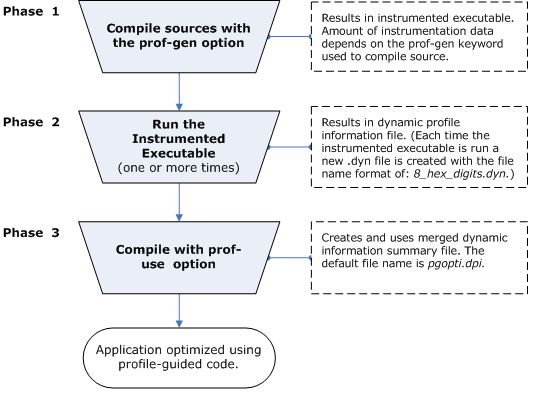
\includegraphics[width=0.5\textwidth]{images/pogo-workflow.jpg}
\end{center}



Or, here, a complete set of steps for actually running it if our program is all in \texttt{main.rs}, from the docs\footnote{\url{https://doc.rust-lang.org/rustc/profile-guided-optimization.html}}:

{\scriptsize
\begin{verbatim}
# STEP 1: Compile the binary with instrumentation
rustc -Cprofile-generate=/tmp/pgo-data -O ./main.rs

# STEP 2: Run the binary a few times, maybe with common sets of args.
#         Each run will create or update `.profraw` files in /tmp/pgo-data
./main mydata1.csv
./main mydata2.csv
./main mydata3.csv

# STEP 3: Merge and post-process all the `.profraw` files in /tmp/pgo-data
llvm-profdata merge -o ./merged.profdata /tmp/pgo-data

# STEP 4: Use the merged `.profdata` file during optimization. All `rustc`
#         flags have to be the same.
rustc -Cprofile-use=./merged.profdata -O ./main.rs
\end{verbatim}
}
(NB: Debian/Ubuntu's rustc doesn't seem to support PGO; I had to rustup it myself on my computer; I also used the Complete Cargo Workflow listed later.)

What does it mean for the executable to be better? We have already looked at an example about how to predict branches. Predicting it correctly will be faster than predicting it incorrectly, but this is not the only thing.  The algorithms will aim for speed in the areas that are ``hot'' (performance critical and/or common scenarios). The algorithms will alternatively aim to minimize the size of code of areas that are ``cold'' (not heavily used). It is recommended in~\cite{pogo} that less than 5\% of methods should be compiled for speed.

It is possible that we can combine multiple training runs and we can manually give some suggestions of what scenarios are important. Obviously the more a scenario runs in the training data, the more important it will be, as far as the POGO optimization routine is concerned, but multiple runs can be merged with user assigned weightings.

\subsection*{Behind the Scenes}

In the optimize phase, the training data is used to do the following optimizations( which I will point out are based on C and \CPP~ programs and not necessarily Rust, but the principles should work because the Rust compiler's approach to this is based on that of LLVM/Clang)~\cite{pogo2}:

\begin{multicols}{2}
\begin{enumerate}
\item Full and partial inlining
\item Function layout
\item Speed and size decision
\item Basic block layout 
\item Code separation
\item Virtual call speculation
\item Switch expansion
\item Data separation
\item Loop unrolling
\end{enumerate}
\end{multicols}

For the most part we should be familiar with the techniques that are listed as being other compiler optimizations we have previously discussed. The new ones are (3) speed and size decision, which we have just covered; and items (4) and (5) which relate to how to pack the generated code in the binary.

According to~\cite{pogo2} the majority of the performance gains relate to the inlining decisions. These decisions are based on the call graph path profiling: the behaviour of function \texttt{foo} may be very different when calling it from \texttt{bar} than it is when calling it from function \texttt{baz}. Let's look at this call graph from~\cite{pogo2}:

\begin{center}
	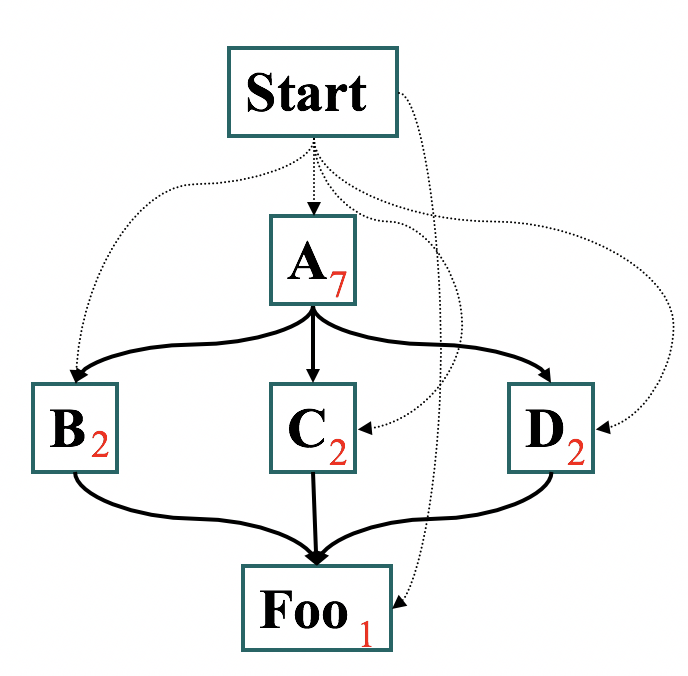
\includegraphics[width=0.25\textwidth]{images/callpaths.png}
\end{center}

Quick analysis of this code would have us find all the ways in which the functions might call each other. In total, there are 14 paths in this code, seven of which get us to function \texttt{Foo}. Consider another diagram showing the relationships between functions, in which the numbers on the edges represent the number of invocations~\cite{pogo2}:

\begin{center}
	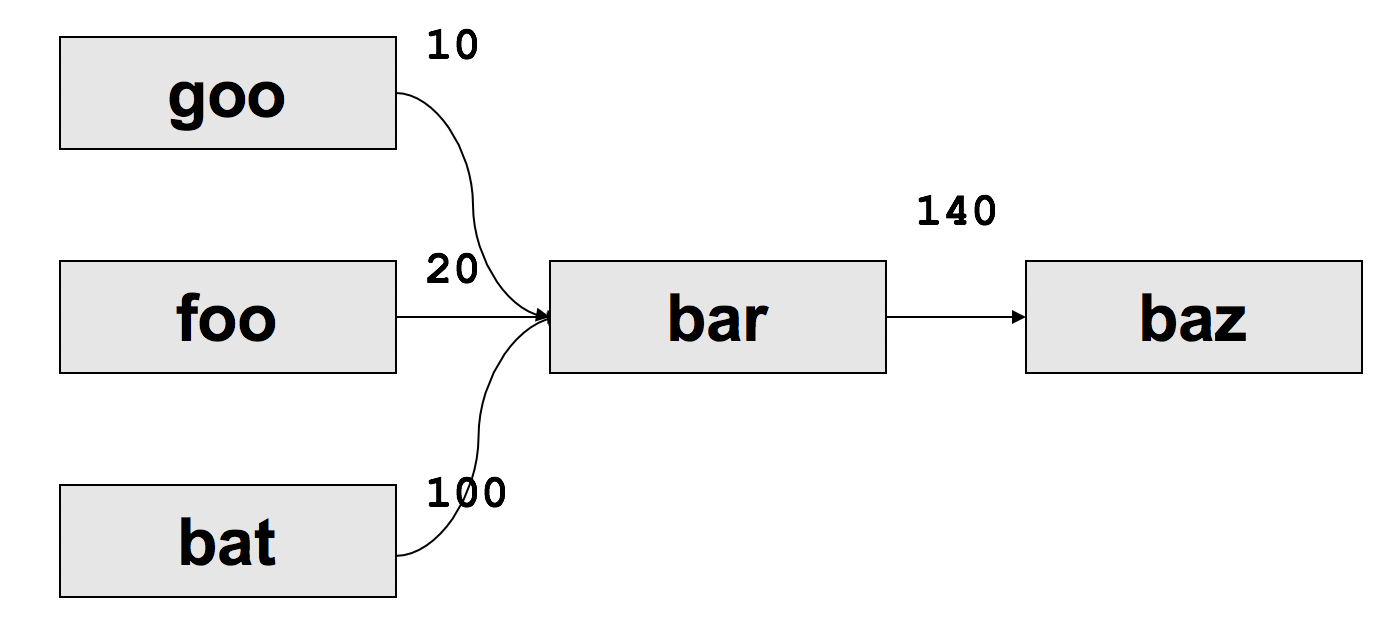
\includegraphics[width=0.4\textwidth]{images/callpaths2.png}
\end{center}

When considering what to do here, POGO takes the view like this~\cite{pogo2}:

\begin{center}
	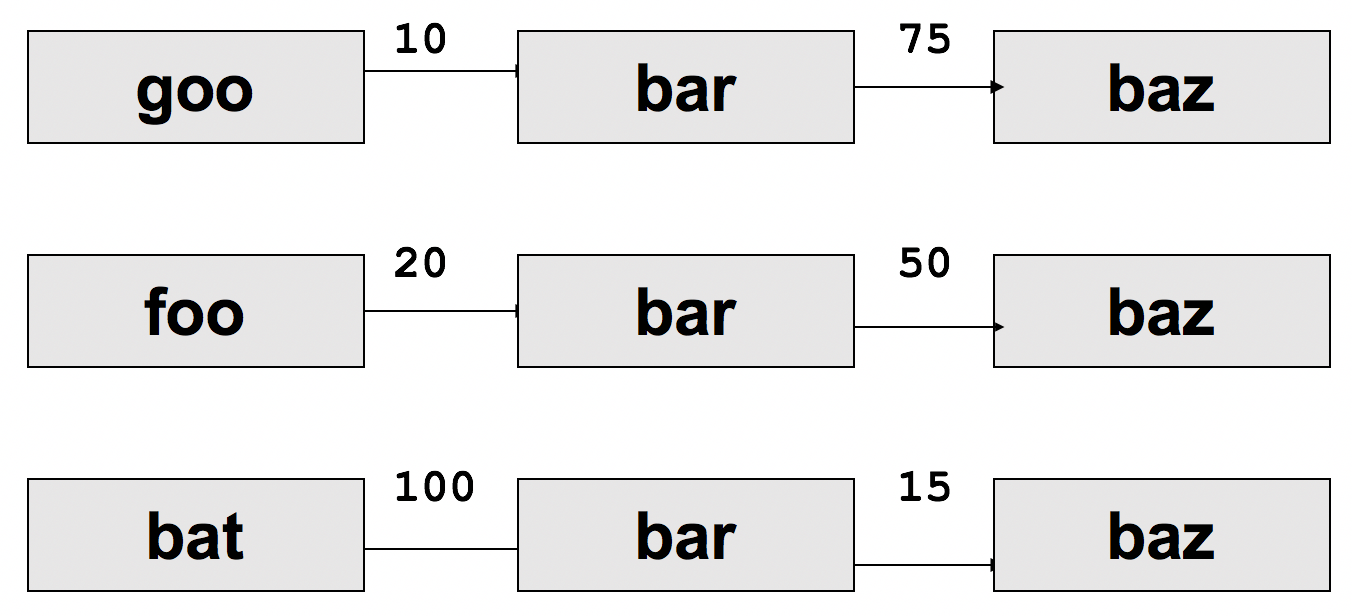
\includegraphics[width=0.4\textwidth]{images/callpaths3.png}
\end{center}

Each part of the call path is considered separately, remembering that we want to inline where it makes sense for speed, but otherwise leave it alone because of code size increases. Inlining \texttt{bar} into \texttt{bat} makes sense, but not inlining \texttt{bar} into \texttt{goo} (because that increases the code size without significant performance benefits). It also makes sense for \texttt{baz} to get inlined into \texttt{bar}. This is illustrated below~\cite{pogo2}:

\begin{center}
	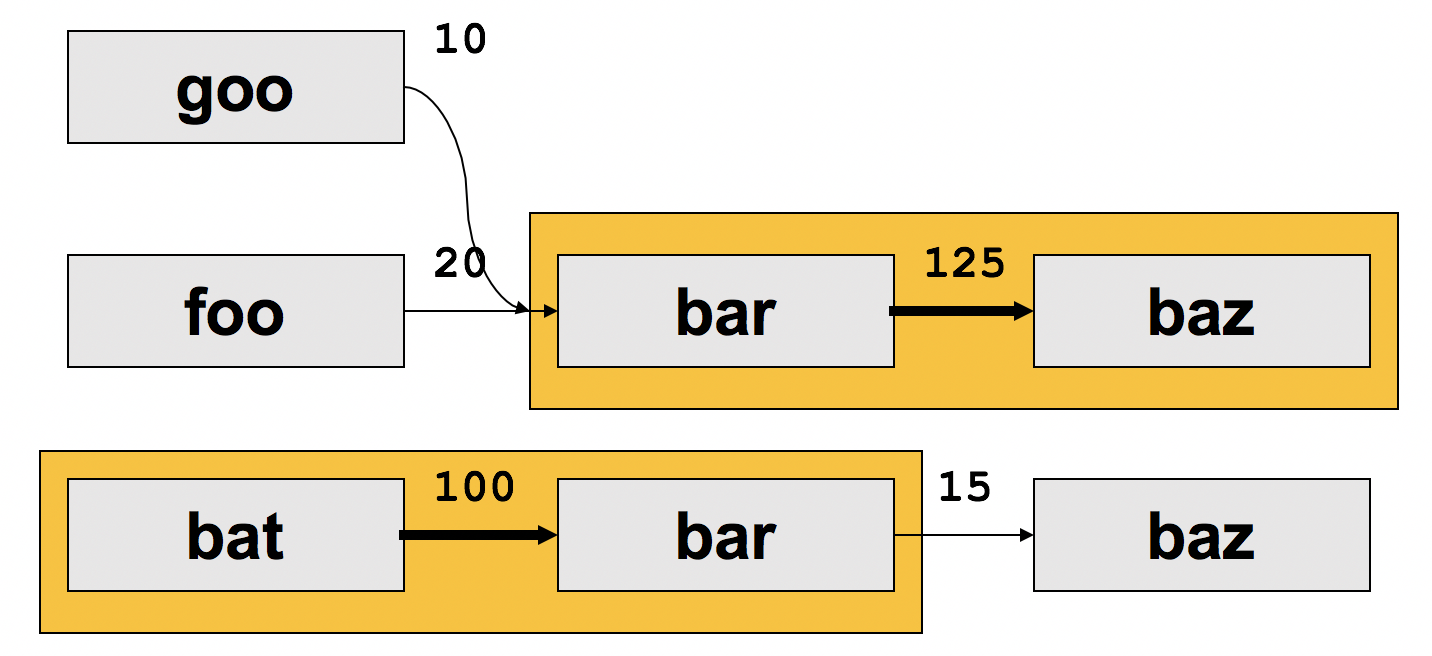
\includegraphics[width=0.4\textwidth]{images/callpaths4.png}
\end{center}

Packing the blocks is also done based on this call graph profiling. The most common cases will be put next to each other, and, where possible, subsequent steps are put next to each other. The more we can pack related code together, the fewer page faults we get by jumping to some other section, causing a cache miss... If the function being called is in the same page as the call, it has achieved ``page locality'' (and that is the goal!). This is represented visually~\cite{pogo2}:

\begin{center}
	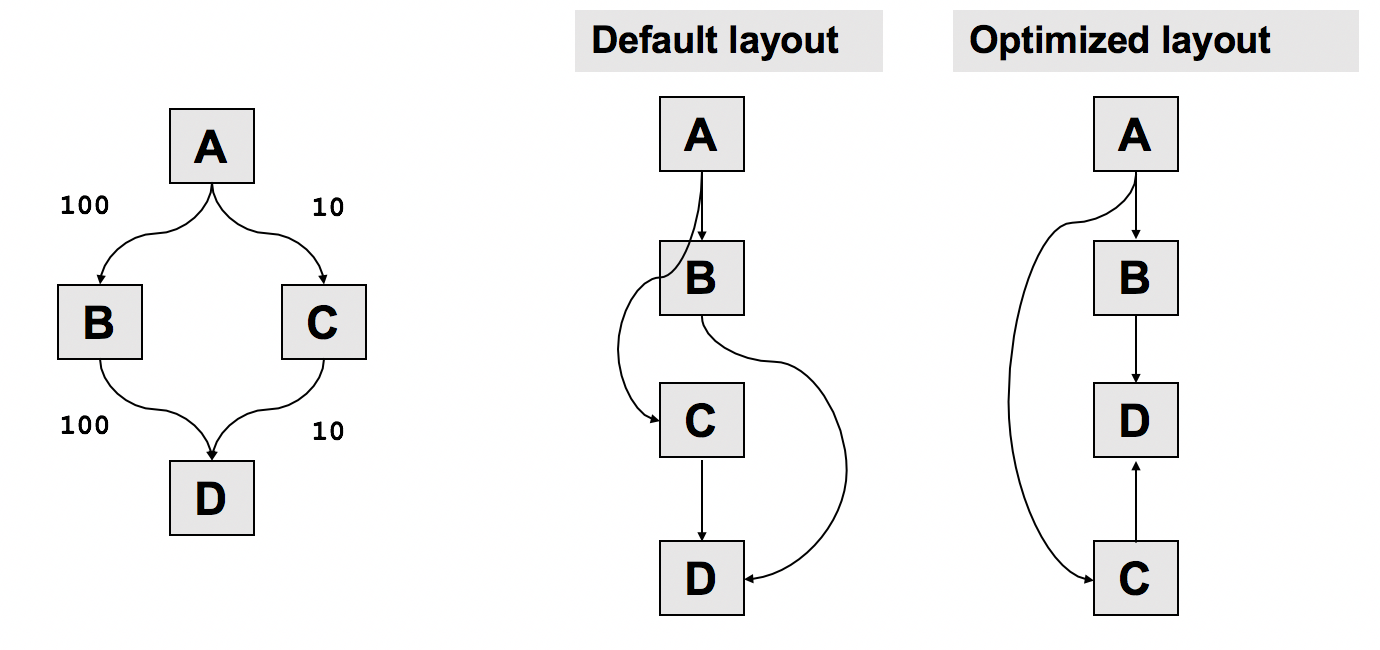
\includegraphics[width=0.6\textwidth]{images/blocklayout.png}
\end{center}

According to the author, the ``dead'' code goes in its own special block. I don't think they actually mean truly dead code, the kind that is compile-time determined to be unreachable, but instead they mean code that never gets invoked in any of the training runs.

So, to sum up, the training data is used to identify what branches are likely to be taken, inlines code where that is a performance increase, and tries to pack the binary code in such a way as to reduce cache misses/page faults. How well does it work?

\subsection*{Benchmark Results}

This table, condensed from~\cite{pogo2} summarizes the gains to be made. The application under test is a standard benchmark suite (Spec2K) (admittedly, C rather than Rust, but the goal is to see if the principle of POGO works and not just a specific implementation):

\begin{center}
\begin{tabular}{l|l|l|l|l|l}
	\textbf{Spec2k:} & \textbf{sjeng} & \textbf{gobmk} & \textbf{perl} & \textbf{povray} & \textbf{gcc}\\ \hline
	\textbf{App Size:} &  {Small} & {Medium} & {Medium} & {Medium} & {Large} \\ \hline
	\textbf{Inlined Edge Count} & 50\% & 53\% & 25\% & 79\% & 65\% \\ \hline
	\textbf{Page Locality} & 97\% & 75\% & 85\% & 98\% & 80\% \\ \hline
	\textbf{Speed Gain} & 8.5\% & 6.6\% & 14.9\% & 36.9\% & 7.9\% \\ 
\end{tabular}
\end{center}

There are more details in the source as to how many functions are used in a typical run and how many things were inlined and so on. But we get enough of an idea from the last row of how much we are speeding up the program, plus some information about why. We can speculate about how well the results in a synthetic benchmark translate to real-world application performance, but at least from this view it does seem to be a net gain.











\chapter*{28 --- Causal and Memory Profiling}

\addcontentsline{toc}{chapter}{28 --- Causal and Memory Profiling}

\section*{Causal Profiling}
At this point we've got some experience in identifying areas of the program that we think are slow or are limiting the maximum performance of our program. If we are presented with more than one thing, how do we know which of those would yield the most benefit? Is it possible that optimizing something would actually have no or a negative effect? The scientific approach would be to do an experiment and find out. That is, change the code, see the impact, re-evaluate. What causal profiling offers us is a way to run those experiments without changing any code. That could be a significant savings of time and effort. 

One such causal profiler is called Coz (pronounced like ``cause'')~\cite{coz}. It does a what-if analysis that says: what would be the impact of speeding up this particular part of the code? 

A very simple approach would just look at the time of the program and just calculate what happens if the runtime of function \texttt{work()} is reduced by, say, 10\%. But that isn't a realistic approach, because speeding up that function might have no overall impact or change the execution time by increasing lock contention or some other mechanism. No, we actually need a simulation. 

The key observation of the Coz profiler authors is the idea that speeding up some area of code is fundamentally the same as slowing down every other part of the code. It's all relative! This is what we would call a virtual speedup. How is the other code slowed down? Adding some pauses to (stopping the execution of) the other threads. That certainly makes them run slower. Maybe you're not convinced that slowing down everything else is equivalent?


Shown below is the argument from~\cite{coz} in visual form. The original runtime is shown as (a). Hypothetically, if we make function \texttt{f} faster by some factor $d = 40\%$ that gives us (b). And if instead of actually making function \texttt{f} faster we instead paused other threads for $0.4 \times t(f)$ where $t(f)$ is the original execution time of \texttt{f}, we get an equivalent effect to that of of optimizing \texttt{f} by $d$.
\begin{center}
	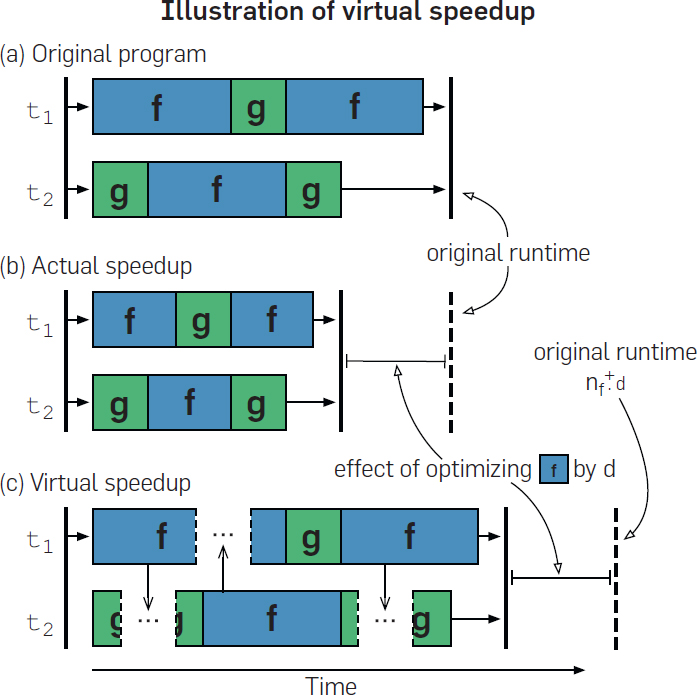
\includegraphics[width=0.4\textwidth]{images/virtual-speedup.jpg}
\end{center}

The tool provides some graphs of potential program speedup. From the recorded presentation, it might look something like the diagram below, where the boxes on the right correspond to different theoretical actions in the application being examined:

\begin{center}
	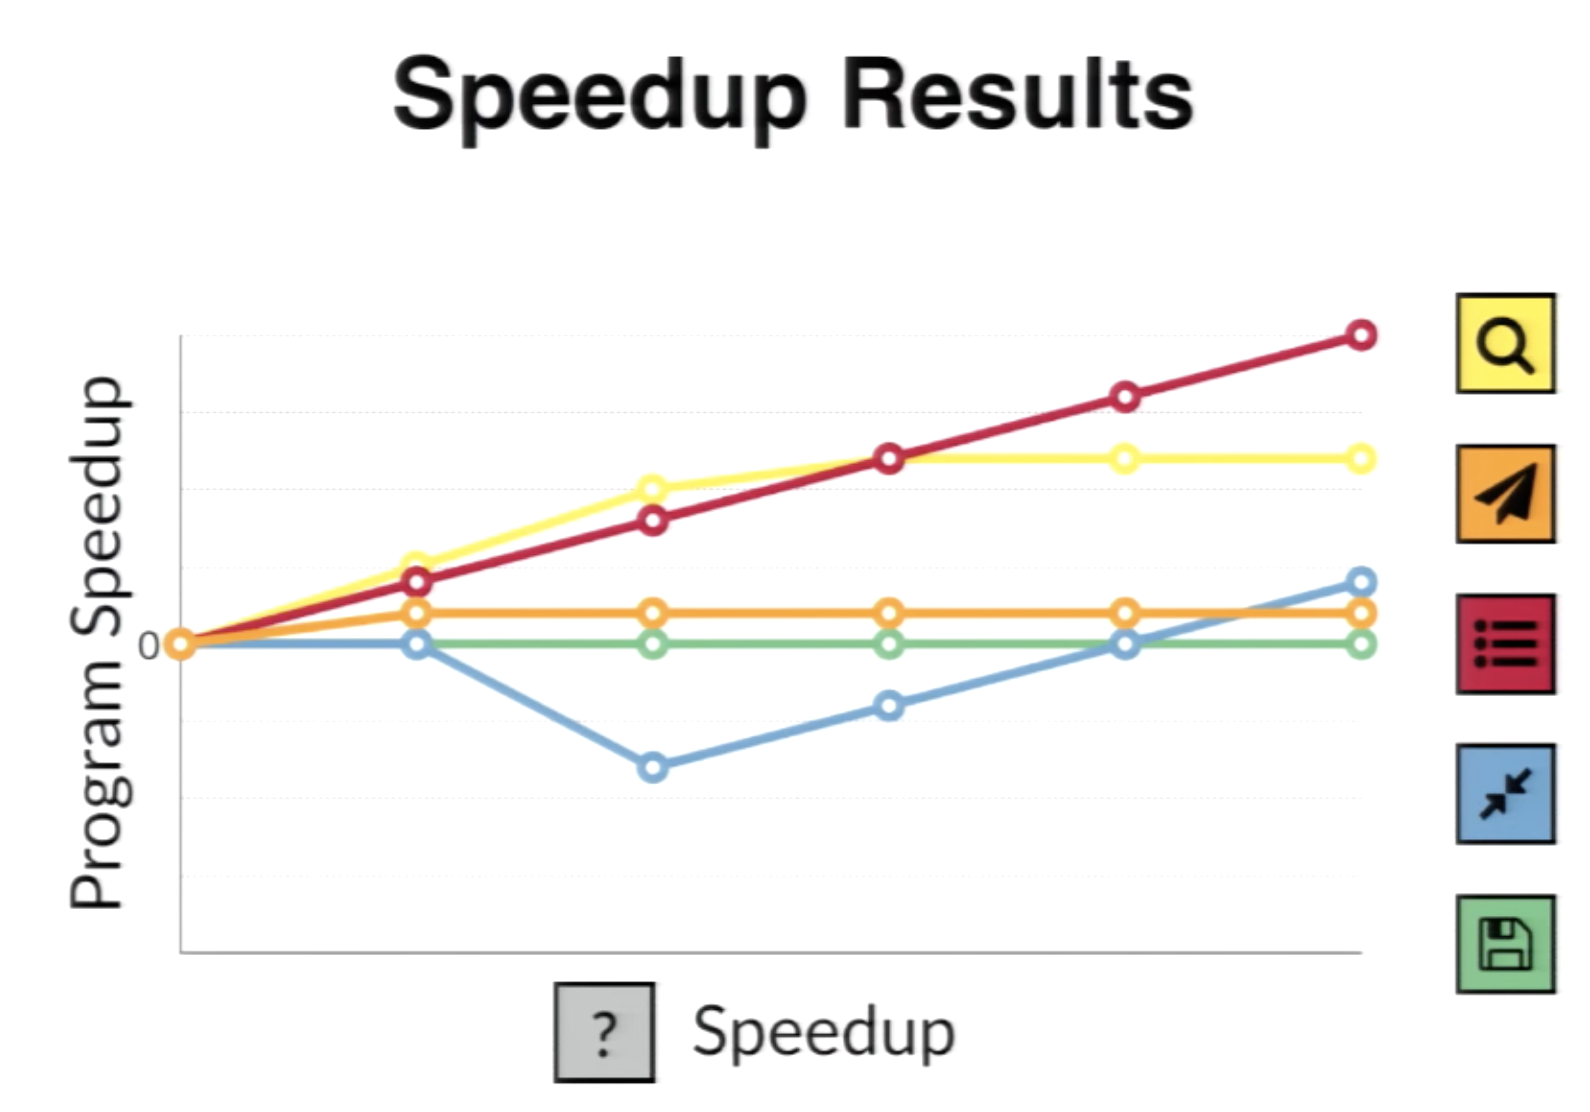
\includegraphics[width=0.4\textwidth]{images/coz-speedup-graph.png}
\end{center}

This pretend application shows all the possible outcomes, from continuous linear speedup, to speedup capped at some point, to no effect, and finally to where optimizing something makes the overall program runtime worse. 

It's easy to imagine scenarios corresponding to each of those. If we're computing the n-body problem, anything that improves the calculation of forces will certainly make things better. And it's easy to imagine that sometimes optimizing a part of the program does not improve anything because that code is not on the critical path. We can also easily imagine that improving something works up to a point where it ceases to be the limiting factor. But making things worse? We already covered that idea: speeding up a thread may increase lock contention or add something to the critical path. At some point, things may recover and be a net benefit.

It is important to remember that just because hypothetically speeding up a particular part of the program would be beneficial, doesn't mean that it's possible to speed up that part. And almost certainly not possible to do so to an arbitrary degree. We still have to make an assessment of what optimizations we can make and how difficult it would be to actually realize those improvements.

Once we've made a change to the program, then it's time to run an experiment again with the new baseline to see what else we can do.

The paper has a table summarizing the optimizations they applied to a few different programs, which seems to support the idea that the tool can be used effectively to get a meaningful speedup with relatively few lines of code~\cite{coz}:
\begin{center}
	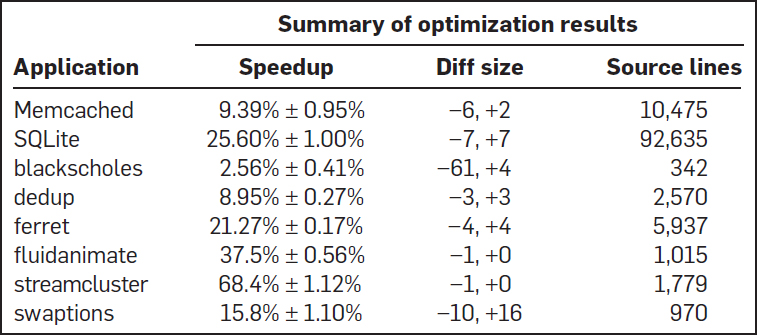
\includegraphics[width=0.6\textwidth]{images/coz-speedup.jpg}
\end{center}

There are potentially some limitations to this, of course. Putting pauses in the execution of the code can work when the execution of the program is all on the same machine and we have control over all the threads; it would need some meaningful extension to work for a distributed system where coordinating things across many servers would be needed.

Using some benchmarking workload, the authors estimate a 17.6\% overhead for this tool, which is broken down into 2.6\% for startup debug information collection, sampling at 4.8\%, and 10.2\% is the delay that's caused by slowing down other threads to create a virtual speedup~\cite{coz}.

If you'd like to see some more details of the tool, you can see the author presentation at the ACM symposium here: \url{https://www.youtube.com/watch?v=jE0V-p1odPg}

\section*{Memory Profiling}

Thus far we have focused on CPU profiling. Other kinds of profiling got some mention, but they're not the only kind of profiling we can do. Memory profiling is also a thing, and specifically we're going to focus on heap profiling.

During Rustification, we dropped a bunch of valgrind content. Valgrind is a memory error and leak detection toolset that is invaluable when programming in \CPP. (In brief: valgrind is a just-in-time engine that reinterprets machine code and instruments it to find sketchy things.) In particular, the memory leaks that valgrind's memcheck tool detects are, for the most part, not possible in Rust unless you try pretty hard\footnote{You can still create cycles in refcounted objects or call \texttt{std::mem::forget} or etc.}---the friendly compiler protects you against them by automatically dropping things.

We're going to look at two kinds of memory profiling here, both part of valgrind. They can both occur in Rust, but it looks like the more common kind is when a lot of memory is allocated and then freed. More completely: ``places that cause excessive numbers of allocations; leaks; unused and under-used allocations; short-lived allocations; and allocations with inefficient data layouts''. valgrind's DHAT tool~\cite[Chapter~10]{valgrind} detects these.

The second kind of memory profiling addresses memory that memcheck reports as ``Still Reachable''. That is, things that remained allocated and still had pointers to them, but were not properly deallocated. Right, we care about them too, and for that we also want to do heap profiling. If we don't look after those things, we're just using more and more memory over time. That likely means more paging and the potential for running out of heap space altogether. Again, the memory isn't really lost, because we could free it.

\subsection*{DHAT}
DHAT tracks allocation points and what happens to them over a program's execution. An allocation point is a point in the program which allocates memory; in C that would be \texttt{malloc}. In Rust there are a bunch of ways to allocate memory, one being \texttt{Box::new}. It aggregates allocation points according to the program stack. Let's first look at a leaf node from the documentation.

\begin{verbatim}
AP 1.1.1.1/2 {
  Total:     31,460,928 bytes (2.32%, 1,565.9/Minstr) in 262,171 blocks (4.41%, 13.05/Minstr), 
     avg size 120 bytes, avg lifetime 986,406,885.05 instrs (4.91% of program duration)
  Max:       16,779,136 bytes in 65,543 blocks, avg size 256 bytes
  At t-gmax: 0 bytes (0%) in 0 blocks (0%), avg size 0 bytes
  At t-end:  0 bytes (0%) in 0 blocks (0%), avg size 0 bytes
  Reads:     5,964,704 bytes (0.11%, 296.88/Minstr), 0.19/byte
  Writes:    10,487,200 bytes (0.51%, 521.98/Minstr), 0.33/byte
  Allocated at {
    ^1: 0x95CACC9: alloc (alloc.rs:72)
      [omitted]
    ^7: 0x95CACC9: parse_token_trees_until_close_delim (tokentrees.rs:27)
    ^8: 0x95CACC9: syntax::parse::lexer::tokentrees::<impl syntax::parse::lexer::
                          StringReader<'a>>::parse_token_tree (tokentrees.rs:81)
    ^9: 0x95CAC39: parse_token_trees_until_close_delim (tokentrees.rs:26)
    ^10: 0x95CAC39: syntax::parse::lexer::tokentrees::<impl syntax::parse::lexer::
                          StringReader<'a>>::parse_token_tree (tokentrees.rs:81)
    #11: 0x95CAC39: parse_token_trees_until_close_delim (tokentrees.rs:26)
    #12: 0x95CAC39: syntax::parse::lexer::tokentrees::<impl syntax::parse::lexer::
                          StringReader<'a>>::parse_token_tree (tokentrees.rs:81)
  }
}
\end{verbatim}

We can see the program point corresponding to this allocation: line 81 of \texttt{tokentrees.rs}.
Furthermore, the most bytes alive at once from this site was 16,779,136: that was 65,543 instances of the
memory allocated here, almost all 256-byte blocks. In total, this allocation site was executed
262,171 times, accounting for 31,460,928 bytes. This information can tell us how important this
allocation site is compared to the entire execution we're inspecting. We can also see how long-lived
the blocks are: on average, a block allocated here lives 4.91\% of the program duration. If instead of
4.91\% we had 0.004\% and a large total, then the allocation point would be excessively transient and perhaps
a good candidate for pooling allocations.

The Reads and Writes lines tell us how often the allocated memory is actually used. In this case,
19\% of the bytes allocated here are ever read, and 33\% are written to. That seems like not many, but if it's something
like a vector that grows, you may not be able to do anything about that. This, however, doesn't look like a vector---you
could check it by looking at the code.

You might also get a super-useful Accesses line if all of the blocks allocated at a site are the same size.
That line tells you how many times each byte in the block was accessed. Zeros, written as dashes (-), are
parts of the block that are never accessed, useful for finding data alignment holes (and hence potential
inefficiencies).

\paragraph{Parents.} Going up the tree, DHAT tells you about all of the allocation points that share a call-stack
prefix. (The \verb+^+ before the number indicates that the line is copied from the parent; a \# indicates that the line is unique to
that node.)

A sibling of the example above would diverge at the call on line 10, not calling
\texttt{parse\_token\_trees\_until\_close\_delim} from line 81 of \texttt{tokentrees.rs}. At the parent, DHAT
reports results for that node and all of its children.

\subsection*{\st{Memory Profiling} Return to Asgard}
JZ generally found a way to talk about Valgrind in previous courses. But now, we're going to use its Massif tool. This is, obviously, a joke on ``massive'', combined with the name Sif, a Norse goddess associated with the earth (and in the Marvel movies, Shieldmaiden to Thor).

So what does Massif do? It will tell you about how much heap memory your program is using, and also how the situation got to be that way. So let's start with the example program from the documentation, badly translated by yours truly to non-idiomatic Rust~\cite{massif}:


\begin{lstlisting}[language=Rust]
fn g() {
    let a = Vec::<u8>::with_capacity(4000);
    std::mem::forget(a)
}

fn f() {
    let a = Vec::<u8>::with_capacity(2000);
    std::mem::forget(a);
    g()
}

fn main() {

    let mut a = Vec::with_capacity(10);
    for _i in 0..10 {
	a.push(Box::new([0;1000]))
    }
    f();
    g();
}
\end{lstlisting}


After we compile, run the command:
{\scriptsize
\begin{verbatim}
plam@amqui ~/c/p/l/l/L/alloc> valgrind --tool=massif target/debug/alloc
==406569== Massif, a heap profiler
==406569== Copyright (C) 2003-2017, and GNU GPL'd, by Nicholas Nethercote
==406569== Using Valgrind-3.16.1 and LibVEX; rerun with -h for copyright info
==406569== Command: target/debug/alloc
==406569== 
==406569== 
\end{verbatim}
}

Doesn't that look useful?! What happened? Your program executed slowly, as is always the case with any of the Valgrind toolset, but you don't get summary data on the console like we did with Valgrind or helgrind or cachegrind. Weird. What we got instead was the file \texttt{massif.out.406569} (matches the PID of whatever we ran). This file, which you can open up in your favourite text editor, is not especially human readable, but it's not incomprehensible like the output from cachegrind (``Aha, a 1 in column 4 of line 2857. That's what's killing our performance!''). There is an associated tool for summarizing and interpreting this data in a much nicer way: \texttt{ms\_print}, which has nothing whatsoever to do with Microsoft. Promise.

If we look at the output there (hint: pipe the output to \texttt{less} or something, otherwise you get a huge amount of data thrown at the console), it looks much more user friendly.

{\scriptsize
\begin{verbatim}
    KB
78.57^                                                                       #
     |                                                                       #
     |                                                                       #
     |                                                                       #
     |                                                                       #
     |                                                                       #
     |                                                                       #
     |                                                                       #
     |                                                                       #
     |                                                                       #
     |                                                                       #
     |                                                                      :#
     |                                                                     @:#
     |                                                                    :@:#
     |                                                                    :@:#
     |                                                                   ::@:#
     |                                                                  :::@:#
     |                                                                  :::@:#
     |                                                                 ::::@:#
     |                                                                :::::@:#
   0 +----------------------------------------------------------------------->ki
     0                                                                   474.1
\end{verbatim}
}

Now wait a minute. This bar graph might be user friendly but it's not exactly what I'd call\ldots useful, is it? For a long time, nothing happens, then\ldots kaboom! According to the docs, what actually happened here is, we gave in a trivial program where most of the CPU time was spent doing the setup and loading and everything, and the trivial program ran for only a short period of time, right at the end. So for a relatively short program we should tell Massif to care more about the bytes than the CPU cycles, with the \verb+--time-unit=B+ option. Let's try that.

{\scriptsize
\begin{verbatim}
    KB
78.57^                                                ##                      
     |                                                # :::                   
     |                                                # :  ::                 
     |                                                # :  : ::               
     |                                       :::::::::# :  : : :::            
     |                                       :        # :  : : :  ::          
     |                                       :        # :  : : :  : ::        
     |                                       :        # :  : : :  : : :::     
     |                              ::::::::::        # :  : : :  : : :  ::   
     |                              :        :        # :  : : :  : : :  : :: 
     |                         ::::::        :        # :  : : :  : : :  : : @
     |                       :::    :        :        # :  : : :  : : :  : : @
     |                    @@@: :    :        :        # :  : : :  : : :  : : @
     |                  ::@  : :    :        :        # :  : : :  : : :  : : @
     |                ::: @  : :    :        :        # :  : : :  : : :  : : @
     |             :::: : @  : :    :        :        # :  : : :  : : :  : : @
     |           :::  : : @  : :    :        :        # :  : : :  : : :  : : @
     |         ::: :  : : @  : :    :        :        # :  : : :  : : :  : : @
     |      :::: : :  : : @  : :    :        :        # :  : : :  : : :  : : @
     |    :::  : : :  : : @  : :    :        :        # :  : : :  : : :  : : @
   0 +----------------------------------------------------------------------->KB
     0                                                                   121.6
\end{verbatim}
}

Neat. Now we're getting somewhere. We can see (from the text below the graph) that 48 snapshots were taken. It will take snapshots whenever there are appropriate allocation and deallocation statements, up to a configurable maximum, and for a long running program, toss some old data if necessary. Let's look in the documentation to see what the symbols mean (they're not just to look pretty). So, from the docs~\cite{massif}:

\begin{itemize}
\item Most snapshots are normal (they have just basic information) They use the `:' characters.

\item Detailed snapshots are shown with `@' characters.  By default, every 10th snapshot is detailed.

\item There is at most one peak snapshot. The peak snapshot is a detailed snapshot, and records the point where memory consumption was greatest. The peak snapshot is represented in the graph by a bar consisting of `\#' characters.
\end{itemize}

As a caveat, the peak can be a bit inaccurate. Peaks are only recorded when a deallocation happens. This just avoids wasting time recording a peak and then overwriting it; if you are allocating a bunch of blocks in succession (e.g. a bunch of structs that have a buffer) then you would constantly be overwriting the peak over and over again. Also, there's some loss of accuracy to speed things up. Well, okay.

So let's look at the snapshots. We'll start with the normal ones. Here are the first 5, numbers 0 through 4:

{\scriptsize
\begin{verbatim}
--------------------------------------------------------------------------------
  n        time(B)         total(B)   useful-heap(B) extra-heap(B)    stacks(B)
--------------------------------------------------------------------------------
  0              0                0                0             0            0
  1            488              488              472            16            0
  2            624              624              592            32            0
  3          1,656            1,656            1,616            40            0
  4          1,768            1,768            1,736            32            0
\end{verbatim}
}

The columns are pretty much self explanatory, with a couple exceptions. The time(B) column corresponds to time measured in allocations thanks to our choice of the time unit at the command line. The extra-heap(B) represents internal fragmentation\footnote{Remember from operating systems: if the user asked for some $n$ bytes where $n$ is not a nice multiple the returned block may be ``rounded up''. So a request for 1000 bytes is bumped up to 1016 bytes in this example. The extra space is ``wasted'' but it's nicer than having a whole bunch of little tiny useless fragments of the heap to be managed.} in the blocks we received. The stacks column shows as zero because by default, Massif doesn't look at the stack. It's a heap profiler, remember?

Number 5 is a ``detailed'' snapshot, so I've separated it out, and reproduced the headers there to make this a little easier to remember what they are.

{
\begin{verbatim}
--------------------------------------------------------------------------------
  n        time(B)         total(B)   useful-heap(B) extra-heap(B)    stacks(B)
--------------------------------------------------------------------------------
  5          1,768            1,768            1,736            32            0
98.19% (1,736B) (heap allocation functions) malloc/new/new[], --alloc-fns, etc.
->57.92% (1,024B) 0x492509B: _IO_file_doallocate (filedoalloc.c:101)
... etc
\end{verbatim}
}

So the additional information we got here is a reflection of where our heap allocations took place. Thus far, all the allocations are associated with the runtime library and {\tt lang\_start}, so not that useful to us.

Then let's look at the peak snapshot (again, trimmed significantly to call out the first thing we need to see here):

{
\begin{verbatim}
--------------------------------------------------------------------------------
  n        time(B)         total(B)   useful-heap(B) extra-heap(B)    stacks(B)
--------------------------------------------------------------------------------
 31         84,072           80,456           80,285           171            0
99.79% (80,285B) (heap allocation functions) malloc/new/new[], --alloc-fns, etc.
->99.53% (80,080B) 0x10F97B: alloc::alloc::alloc (alloc.rs:81)
| ->49.82% (40,080B) 0x10F771: <alloc::alloc::Global as core::alloc::Alloc>::alloc (alloc.rs:169)
| | ->49.72% (40,000B) 0x10D90D: alloc::raw_vec::RawVec<T,A>::allocate_in (raw_vec.rs:88)
| | | ->49.72% (40,000B) 0x10D744: alloc::raw_vec::RawVec<T>::with_capacity (raw_vec.rs:140)
| | |   ->49.72% (40,000B) 0x10C412: alloc::vec::Vec<T>::with_capacity (vec.rs:355)
| | |     ->39.77% (32,000B) 0x10FCF2: alloc::g (main.rs:2)
| | |     | ->19.89% (16,000B) 0x10FD5F: alloc::f (main.rs:9)
\end{verbatim}
}

Massif has found all the allocations in this program and distilled them down to a tree structure that traces the path through which all of these various memory allocations occurred. So not just where the \texttt{malloc} call happened, but also how we got there. With lots of Rust helper functions as well.

If I ask valgrind what it thinks of this program, it says:

{\scriptsize
\begin{verbatim}
plam@amqui ~/c/p/l/l/L/alloc> valgrind target/debug/alloc
==406822== Memcheck, a memory error detector
==406822== Copyright (C) 2002-2017, and GNU GPL'd, by Julian Seward et al.
==406822== Using Valgrind-3.16.1 and LibVEX; rerun with -h for copyright info
==406822== Command: target/debug/alloc
==406822== 
==406822== 
==406822== HEAP SUMMARY:
==406822==     in use at exit: 40,000 bytes in 3 blocks
==406822==   total heap usage: 25 allocs, 22 frees, 82,177 bytes allocated
==406822== 
==406822== LEAK SUMMARY:
==406822==    definitely lost: 40,000 bytes in 3 blocks
==406822==    indirectly lost: 0 bytes in 0 blocks
==406822==      possibly lost: 0 bytes in 0 blocks
==406822==    still reachable: 0 bytes in 0 blocks
==406822==         suppressed: 0 bytes in 0 blocks
==406822== Rerun with --leak-check=full to see details of leaked memory
==406822== 
==406822== For lists of detected and suppressed errors, rerun with: -s
==406822== ERROR SUMMARY: 0 errors from 0 contexts (suppressed: 0 from 0)
\end{verbatim}
}

We used to say: ``So probably a good idea to run valgrind first and make it happy before we go into figuring out where heap blocks are going with Massif.'' Now, well, just use Rust and then DHAT. But Massif is still another tool at your disposal. Okay, what to do with the information from Massif, anyway? It should be pretty easy to act upon this information. Start with the peak snapshot (worst case scenario) and see where that takes you (if anywhere). You can probably identify some cases where memory is hanging around unnecessarily. 

Things to watch out for:
\begin{itemize}
\item memory usage climbing over a long period of time, perhaps slowly, but never really decreasing---memory is filling up somehow with some junk? 
\item large spikes in the graph---why so much allocation and deallocation in a short period?
\end{itemize}

Other cool things we can do with Massif~\cite{massif}:

\begin{itemize}
	\item Look into stack allocation (\verb+--stacks=yes+) option. This slows stuff down a lot, and not really necessary since we want to look at heap.
	\item Look at the children of a process (anything split off with \texttt{fork}) if desired.
	\item Check low level stuff: if we're doing something other than \texttt{malloc}, \texttt{calloc}, \texttt{new}, etc. and doing low level stuff like \texttt{mmap} or \texttt{brk} that is usually missed, but we can do profiling at page level (\verb+--pages-as-heap=yes+).
\end{itemize}

% which programs to live demo?
As is often the case, we have examined how the tool works on a trivial program. As a live demo, well, tune in and be surprised!
%let's see what happens when we take the program complexity up a little bit by (1) looking at the search program we saw in the earlier talk about valgrind; and (2) looking at the original (unmodified) paster.c file from assignment 1 (and then perhaps fixing it and going on). Depending on time available, we may look at some more complex programs.









\chapter*{29 --- Liar, Liar}

\addcontentsline{toc}{chapter}{29 --- Liar, Liar}

I was thinking today about how humans are quite adept at building and
using tools (though not
unique\footnote{https://www.rnz.co.nz/news/national/366747/clever-kea-using-tools-to-raid-traps}). Profilers
are useful tools, but they can mislead you.  If you understand how
profilers work, you can avoid being misled.

As we've been saying this week, there are sampling-based and instrumentation-based profilers.
The tl;dr is that a sampling-based profiler can miss things, while an instrumentation-based
profiler distorts the system under observation.

Visually, sampling-based profiling can do this:
\begin{center}
	\url{https://www.youtube.com/watch?v=jQDjJRYmeWg}
\end{center}

The video's not fake; it's a real helicopter and it's really flying. What's happening, however, is that the camera is taking images at some multiple of the frequency of the blade rotation speed so it gives the illusion that the blades are not spinning at all. This is a sampling problem, and you see the same problem in car commercials on TV where it looks like the wheels are spinning backwards. They're not, but the sampling effect of the camera can make it look that way.

The main assumptions underlying sampling are that samples are ``random'' and that the sample distribution approximates the actual time-spent distribution\footnote{Lifted from ``Profilers are Lying Hobbitses'', \url{https://www.infoq.com/presentations/profilers-hotspots-bottlenecks/}, which talks about profiling for JVMs.}.

\section*{Lies from Metrics}
While app-specific metrics can lie too, mostly we'll talk about CPU
perf counters today.
In particular, we're going to look at two types of sampling-based lies.

The reference for the first type of lie is a blog post by Paul Khuong~\cite{metrics}.

This goes back to {\tt mfence}, which we've seen before. It is used, for instance, in
spinlock implementations. Khuong found that his profiles said that spinlocking didn't take much time.
But empirically: eliminating spinlocks = better than expected! Hmm.

The next step is (as we do in this course) to create microbenchmarks to better understand what's
going on. The microbenchmark contained memory accesses to uncached locations, or computations,
surrounded by store pairs/mfence/locks. He used perf to evaluate the impact of mfence vs lock.
You'll recall that perf is sampling-based and records how often the CPU is found executing each
instruction.

{\scriptsize
\begin{lstlisting}
# for locks:
$ perf annotate -s cache_misses
[...]
    0.06 :        4006b0:       and    %rdx,%r10
    0.00 :        4006b3:       add    $0x1,%r9
    ;; random (out of last level cache) read
    0.00 :        4006b7:       mov    (%rsi,%r10,8),%rbp
   30.37 :        4006bb:       mov    %rcx,%r10
    ;; foo is cached, to simulate our internal lock
    0.12 :        4006be:       mov    %r9,0x200fbb(%rip)
    0.00 :        4006c5:       shl    $0x17,%r10
    [... Skipping arithmetic with < 1% weight in the profile]
    ;; locked increment of an in-cache "lock" byte
    1.00 :        4006e7:       lock incb 0x200d92(%rip)
   21.57 :        4006ee:       add    $0x1,%rax
    [...]
    ;; random out of cache read
    0.00 :        400704:       xor    (%rsi,%r10,8),%rbp
   21.99 :        400708:       xor    %r9,%r8
    [...]
    ;; locked in-cache decrement
    0.00 :        400729:       lock decb 0x200d50(%rip)
   18.61 :        400730:       add    $0x1,%rax
    [...]
    0.92 :        400755:       jne    4006b0 <cache_misses+0x30>
\end{lstlisting}
}

We can see that in the lock situation, reads take 30 + 22 = 52\% of runtime,
while locks take 19 + 21 = 40\% of runtime.

{\scriptsize
\begin{lstlisting}
# for mfence:
$ perf annotate -s cache_misses
[...]
    0.00 :        4006b0:       and    %rdx,%r10
    0.00 :        4006b3:       add    $0x1,%r9
    ;; random read
    0.00 :        4006b7:       mov    (%rsi,%r10,8),%rbp
   42.04 :        4006bb:       mov    %rcx,%r10
    ;; store to cached memory (lock word)
    0.00 :        4006be:       mov    %r9,0x200fbb(%rip)
    [...]
    0.20 :        4006e7:       mfence 
    5.26 :        4006ea:       add    $0x1,%rax
    [...]
    ;; random read
    0.19 :        400700:       xor    (%rsi,%r10,8),%rbp
   43.13 :        400704:       xor    %r9,%r8
    [...]
    0.00 :        400725:       mfence 
    4.96 :        400728:       add    $0x1,%rax
    0.92 :        40072c:       add    $0x1,%rax
    [...]
    0.36 :        40074d:       jne    4006b0 <cache_misses+0x30>
\end{lstlisting}
}
Looks like the reads take 85\% of runtime,
while the mfence takes 15\% of runtime.

Metrics lie, though, and when you focus on the metrics as opposed to what you
actually care about, it's easy to be led astray.

In this case, what we actually care about is the total \# of cycles.

    \begin{tabular}{lr}
    No atomic/fence:& 2.81e9 cycles\\
    lock inc/dec: & 3.66e9 cycles\\
    mfence: & 19.60e9 cycles
    \end{tabular}

That 15\% number is a total lie.
Profilers, even using CPU expense counts, drastically underestimate the impact of mfence,
and overestimate the impact of locks.

This is because mfence causes a pipeline flush, and the resulting 
costs get attributed to instructions being flushed, not to the mfence itself. In other
words, mfence makes other instructions run more slowly, which camouflages its own effect
on the overall performance.


\section*{The Long Tail}

The other type of lie that sampling can hide is the one where infrequent long tails are hidden in averages.
Our source here is the blog post by Dan Luu~\cite{perf-tracing}. Suppose we have a task that's going to get distributed over multiple computers (like a search). If we look at the latency distribution, the problem is mostly that we see a long tail of events and when we are doing a computation or search where we need all the results, we can only go as the slowest step. Let's take a look at a histogram of disk read latencies, where we are performing a 64 kB read, also from that source:

\begin{center}
	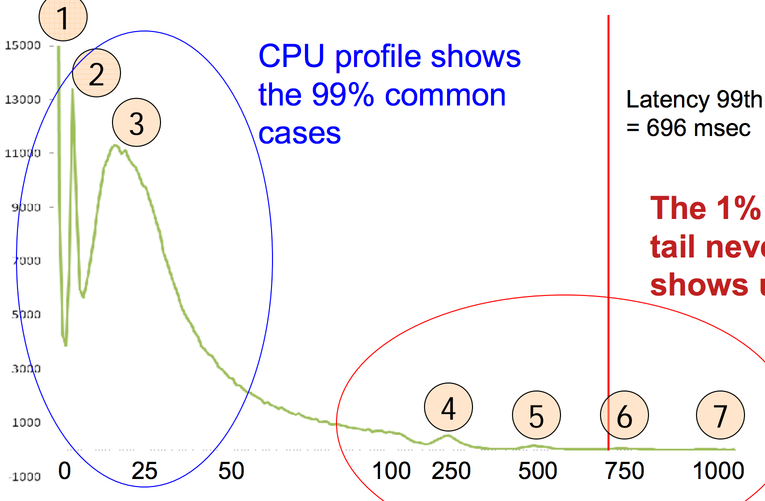
\includegraphics[width=0.5\textwidth]{images/disk_tail.png}
\end{center}

Let's break it down. Peak 1 corresponds to something cached in RAM---best case scenario. Peak 2 is at around 3ms, which is too fast for spinning and seeking magnetic hard disks, but it's fast enough for reading something from the disk cache via the PCI-Express interface. Peak 3 is obviously disk seek and read times, around 25ms. 

These numbers don't look terrible, except for the fact that we have peaks at 250, 500, 750, and 1000 ms and the 99th percentile is some 696ms which is a very, very long time. Sampling profilers are not very good at finding these things, because they throw everything into various buckets and therefore we get averages. The averages are misleading, though, because we have these weird outliers that take dramatically longer. Averages are nice as long as our data is also reasonably ``nice''.

So what actually happened? Well, from~\cite{perf-tracing}: The investigator found out that the cause was kernel throttling of the CPU for processes that went beyond their usage quota. To enforce the quota, the kernel puts all of the relevant threads to sleep until the next multiple of a quarter second. When the quarter-second hand of the clock rolls around, it wakes up all the threads, and if those threads are still using too much CPU, the threads get put back to sleep for another quarter second. The phase change out of this mode happens when, by happenstance, there aren't too many requests in a quarter second interval and the kernel stops throttling the threads. After finding the cause, an engineer found that this was happening on 25\% of disk servers at Google, for an average of half an hour a day, with periods of high latency as long as 23 hours. This had been happening for three years.

Further limitations of sampling profilers emerge, as demonstrated in this graph, also from~\cite{perf-tracing}, showing the data we get out of our sampling profiler if we take a look at Lucene (a search indexer):

\begin{center}
	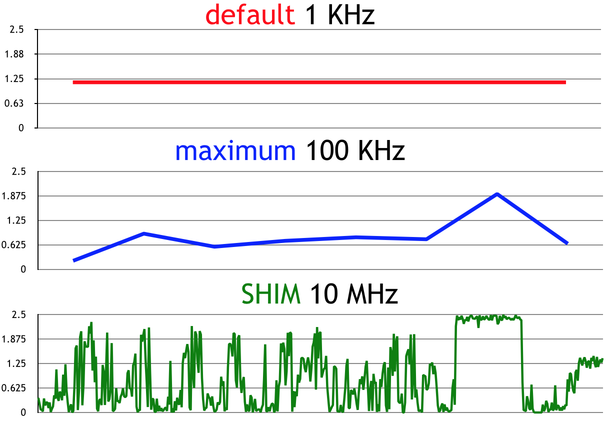
\includegraphics[width=0.3\textwidth]{images/perf-sample.png}
\end{center}

So at the default sampling interval for perf we see\ldots nothing interesting whatsoever. If we bump up to the max sampling frequency of perf, we get a moderately more interesting graph, but not much. If we use a different tool and can sample at a dramatically higher rate, then we end up with something way more useful. So we're left to wonder why does perf sample so infrequently, and how does SHIM get around this?

Well, for one thing, perf samples are done with interrupts. Processing interrupts takes a fair amount of time and if you crank up the rate of interrupts, before long, you are spending all your time handling the interrupts rather than doing useful work. So sampling tools usually don't interrupt the program too often. SHIM gets around this by being more invasive---it instruments the program, adding some periodically executed code that puts information out whenever there is an appropriate event (e.g., function return). This produces a bunch of data which can be dealt with later to produce something useful.

This instrumentation-based approach is more expensive in general, but note that DTrace\footnote{Note also the comment in the blog post: ``Yes, that includes dtrace, which I'm calling out in particular because any time you have one of these discussions, a dtrace troll will come along to say that dtrace has supported that for years. It's like the common lisp of trace tools, in terms of community trolling.''} and Nethercote's counts tool (discussed in L25) also enable custom instrumentation of select events. 

\section*{Lies from Counters}
This is fairly niche, but Rust compiler hackers were trying to include
support for hardware performance counters (what perf reports) because
{\tt -Z self-profile} data was too noisy\footnote{Full story, in gory
detail,
at \url{https://hackmd.io/sH315lO2RuicY-SEt7ynGA?view}.}. Counters
are, for instance, faster than measuring time and way (i.e. 5 orders of magnitude) more deterministic.

To make counters as deterministic as possible:
\begin{itemize}[noitemsep]
\item disable Address Space Layout Randomization (randomized pointer addresses affect hash layouts);
\item subtract time spent processing interrupts (IRQs);
\item profile one thread only (if you can, in your context).
\end{itemize}
Fun fact. We talked about Spectre back in Lecture 7. Speculative execution comes up here too in terms of
counters being wrong. AMD speculates past atomics and then rolls back, but doesn't roll back perf counters.
Post-Spectre, there's a hidden model-specific register (``SpecLockMap'') that disables speculating past atomics, the kind of thing you would
want around to protect you against future things in that vein that someone might discover. Or, in better words than mine\footnote{\url{https://twitter.com/eddyb_r/status/1323587371703668742}}:

\begin{center}
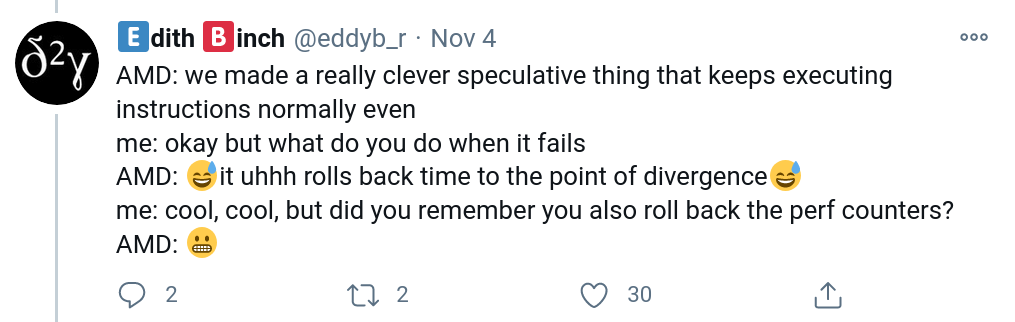
\includegraphics{images/L27-eb-tweet.png}
\end{center}

\section*{Lies about Calling Context}
This part is somewhat outdated now, as it's a pretty specific technical problem that especially arises under the {\tt gprof} tool. It's still a good example of lying tools, though,
so I'll include a condensed version. Yossi Kreinin~\cite{lies} writes about it in more detail.

gprof uses two C standard-library functions: {\bf profil()} and {\bf mcount()}.

\vspace*{-1em}
\begin{itemize}[noitemsep]
\item {\bf profil()}: asks glibc to record which instruction 
  is currently executing (100$\times$/second).
\item {\bf mcount()}: records call graph edges; called by {\tt -pg} instrumentation.
\end{itemize}
\vspace*{-1em}

Hence, {\bf profil} information is statistical, while {\bf mcount}
information is exact.  gprof can draw unreliable inferences. If you have a method \texttt{easy} and a method \texttt{hard}, each of which is called once, and \texttt{hard} takes up almost all the CPU time,
gprof might divide total time by 2 and report bogus results.

The following results from gprof are suspect (among others):
\vspace*{-1em}
\begin{itemize}[noitemsep]
  \item contribution of children to parents;
  \item total runtime spent in self+children;
\end{itemize}
\vspace*{-1em}

\paragraph{When are call graph edges right?}
Two cases:
\vspace*{-1em}
    \begin{itemize}[noitemsep]
    \item functions with only one caller
      (e.g. {\tt f()} only called by {\tt g()}); or,
    \item functions which always take the same time to complete
      (e.g. {\tt rand()}).
    \end{itemize}
\vspace*{-1em}

On the other hand, results for any function whose running time depends on its inputs,
and which is called from multiple contexts, are sketchy.


Next, we'll talk about callgrind/KCacheGrind. Like our old friends memcheck, helgrind, and cachegrind, callgrind is part of valgrind, and runs the program under an x86 JIT.  KCacheGrind is a frontend to callgrind. callgrind gives better information, but imposes
more overhead.
KCacheGrind works properly on the earlier running example, but we can still deceive it with more complicated examples.

%% \paragraph{Summary.} We've seen that some profiler results are exact;
%% some results are sampled; and some results are interpolated. If you understand the tool, you understand where it can go
%% wrong. 

%% Understand your tools!


\paragraph{Overall summary.} We saw a bunch of lies today: calling-context lies and perf attribution
lies. To avoid being bitten by lies, remember to focus on the metric you actually care about,
and understand how your tools work.










\chapter*{30 --- Clusters \& Cloud Computing}

\addcontentsline{toc}{chapter}{30 --- Clusters \& Cloud Computing}

\section*{Clusters and Cloud Computing}
Almost everything we've seen so far has improved performance on a single
computer. Sometimes, you need more performance than you can get on a
single computer, or you have reached a point where it's a lot better value for
your money to buy two cheap computers than one very expensive computer.
For the most part, if you could split your problem into
multiple threads or multiple processes, you can do the same with multiple
computers. We'll survey techniques for programming for
performance using multiple computers; although there's overlap with
distributed systems, we're looking more at calculations here.

\paragraph*{Message Passing.} Rust encourages message-passing, but
a lot of your previous experience when working with C may have centred around
shared memory systems and you may have done that in Rust too (\texttt{Mutex}, 
anyone?). In some circumstances that we've seen, you don't have a choice!
The model of GPU programming meant we had to explicitly
manage copying of data. When we have multiple computers, shared memory is not
an option, so we have to use message passing. Fortunately, we know how to do
that. The only thing to note now is that communication over the network is
much more expensive than communicating within the same system, so we will
need to think carefully about how much to communicate.

There was a time when we would talk about MPI, the \emph{Message Passing 
Interface}, a de facto standard for programming message-passing multi-
computer systems. This is, unfortunately, no longer the way. 
MPI sounds good, but in practice people tend to use other things. 
Here's a detailed piece about the relevance of MPI today:~\cite{hpcmpi}, if 
you are curious. 

\paragraph{REST}
We've already seen asynchronous I/O using HTTP (curl) which we could use to
consume a REST API as one mechanism for multi-computer communication. You
may have also learned about sockets and know how to use those, which would
underlie a lot of the mechanisms we're discussing. The socket approach is too
low-level for what we want to discuss, while the REST API approach is at a
reasonable level of abstraction. 

REST APIs are often completely synchronous, but don't have to be: 
you can set up  callbacks to be notified when a computation is done, or
the caller can check back later to see if the request is finished. But these
aren't truly asynchronous, because the remote machine has to be available at
the time of each call. Perhaps we'd like to decouple services even more than
that and use something else...

\paragraph{Kafka.} 
Let's talk about Apache Kafka, a self-described ``distributed streaming platform'' that's got significant adoption in industry as a mechanism of communication between different services running over a network. We're using~\cite{kafka} as a guide and it provides a breakdown on how Kafka works.

Communication is based around the idea of producers writing a record (some data element, like an invoice) into a topic (categorizing messages) and consumers taking the item from the topic and doing something useful with it. A message remains available for a fixed period of time and can be replayed if needed. I think at this point you have enough familiarity with the concept of the producer-consumer problem and channels/topics/subscriptions that we don't need to spend a lot of time on it. 


Kafka's basic strategy is to write things into an immutable log. The log is split into different partitions; you choose how many when creating the topic, where more partitions equals higher parallelism. The producer writes something and it goes into one of the partitions. Consumers read from each one of the partitions and writes down its progress (``commit its offset'') to keep track of how much of the topic it has consumed.  See this image from \url{kafka.apache.org}:

\begin{center}
	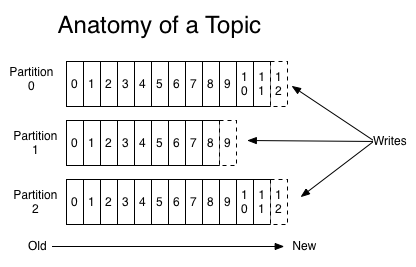
\includegraphics[width=0.4\textwidth]{images/kafka-partition.png}
\end{center}

The nice part about such an architecture is that we can provision the parallelism that we want, and the logic for the broker (the system between the producer and the consumer, that is, Kafka) is simple. Also, consumers can take items and deal with them at their own speed and there's no need for consumers to coordinate; they manage their own offsets. Messages are removed from the topic based on their expiry, so it's not important for consumers to get them out of the queue as quickly as possible.

You can see a visualization of Kafka at \href{https://softwaremill.com/kafka-visualisation/}{https://softwaremill.com/kafka-visualisation/}.

Quick aside on that: under normal circumstances, in something like a standard queue, there's a little bit of pressure to get items out of the queue quickly. If the queue is growing, it might mean the queue is full and new items can't be produced or are thrown away... or perhaps you get charged money for the storage space the queue is using. 

You might think that it's a solution to take the item out of the queue in one transaction and then process it later. That's okay only if you've successfully saved it to a database or other persistent storage. Otherwise, you could take the item out and a crash or called shutdown means that the item doesn't actually get processed. Oops!

\paragraph{Alternatives.} There's also some popular AWS (Amazon Web Services)-based solutions for this kind of multiple computer communication: SNS (Simple Notification Service) and SQS (Simple Queueing Service). They are, broadly speaking, just other ways to decouple the communication of your programs.

SNS is good for sending lots of messages to multiple receivers, maybe push notifications or making sure all systems update their records or that you send pager alerts to people about things that have gone wrong. SNS messages are not persistent, so if you miss it, you miss it. 

SQS is more for batches of work where it's not particularly time-sensitive and the item will be consumed by a worker. SQS data is deleted after being taken out of the queue and may or may not have ordering guarantees. SQS does have limits on how long a message can be stored, though. 

\subsection*{Cloud Computing}
We'll start with a little bit of history.
In the old days, if you wanted a cluster, you had to find a bunch of
money to buy and maintain a pile of expensive machines. Not anymore.
Cloud computing is perhaps way overhyped, but we can talk about 
one particular aspect of it, as exemplified by Amazon's Elastic
Compute Cloud (EC2).

Consider the following evolution:
\begin{itemize}
\item Once upon a time, if you wanted a dedicated server on the
  Internet, you had to get a physical machine hosted, usually in a
  rack somewhere. Or you could live with inferior shared hosting.
\item Virtualization meant that you could instead pay for part of a
  machine on that rack, e.g. as provided by {\tt slicehost.com}.  This
  is a win because you're usually not maxing out a computer, and you'd
  be perfectly happy to share it with others, as long as there are
  good security guarantees. All of the users can get root access to their virtual part computer.
  (Unfortunately, Spectre and Meltdown allow you to see parts of the machine that are not yours.)
\item Clouds enable you to add more machines on-demand. Instead of
  having just one virtual server, you can spin up dozens (or
  thousands) of server images when you need more compute
  capacity. These servers typically share persistent storage, also in
  the cloud. 
\end{itemize}

In cloud computing, you pay according to the number of machines, or
instances, that you've started up. Providers offer different instance
sizes, where the sizes vary according to the number of cores, local
storage, and memory. Some instances even have GPUs, but it seemed 
uneconomic to use this for Assignment 3, at least in previous years (I
have not done the calculation this year). 
Instead we have the {\tt ecetesla} machines.

\paragraph{Launching Instances.} When you need more compute power,
you launch an instance. The input is a virtual machine image.  You use
a command-line or web-based tool to launch the instance.  After you've
launched the instance, it gets an IP address and is
network-accessible. You have full root access to that instance.

Amazon provides public images which run a variety of operating
systems, including different Linux distributions, Windows Server, and
OpenSolaris. You can build an image which contains the software you
want, including Hadoop and OpenMPI.

\paragraph{Terminating Instances.} A key part of cloud computing is
that, once you no longer need an instance, you can just shut it down
and stop paying for it. All of the data on that instance goes away.

\paragraph{Continuous Deployment.} The combination of launching and terminating instances can mean that updates don't require downtime: you start up the new instances and then shut down the old ones so there's no gap where the service is down.

Sometimes this causes slight headaches, like if you make a database change that's incompatible: the old nodes will have a problem, so you need to be a little careful with this.

\paragraph{Storing Data.} You probably want to keep some persistent results
from your instances. Basically, you can either mount a storage device,
also on the cloud (e.g. Amazon Elastic Block Storage); or, you can
connect to a database on a persistent server (e.g. Amazon SimpleDB or
Relational Database Service); or, you can store files on the Web
(e.g. Amazon S3). 


\section*{Clusters versus Laptops}
There is a paper about this: Frank McSherry, Michael Isard, Derek G. Murray. ``Scalability! But at what COST?'' HotOS XV. This part of the lecture is based on the companion blog post~\cite{scalecost}.

The key idea: scaling to big data systems introduces substantial overhead. Let's just see how, say, a laptop compares, in absolute times, to 128-core big data systems.

\paragraph{Summary.} Big data systems haven't yet been shown to be obviously good; current evaluation is lacking.
The important metric is not just scalability; absolute
performance matters a lot too. We don't want a situation where we are just scaling up to $n$ systems to deal with the complexity of scaling up to $n$ systems. Or, as Oscar Wilde put it: ``The bureaucracy is expanding to meet the needs of the expanding bureaucracy.''

\paragraph{Methodology.} We'll compare a competent single-threaded implementation to top
big data systems, as described in an OSDI 2014 (top OS conference) paper on GraphX~\cite{graphx}. The domain: graph processing
algorithms, namely PageRank and graph connectivity (for which the bottleneck is label propagation). The subjects: graphs with billions of edges, amounting to a few
GB of data.

\paragraph{Results.} 128 cores don't consistently beat a laptop at PageRank: e.g. 249--857s on the twitter\_rv dataset for the big data system vs 300s for the laptop, and they are 2$\times$ slower for label
propagation, at 251--1784s for the big data system vs 153s on
twitter\_rv. From the blogpost:

\begin{center}
	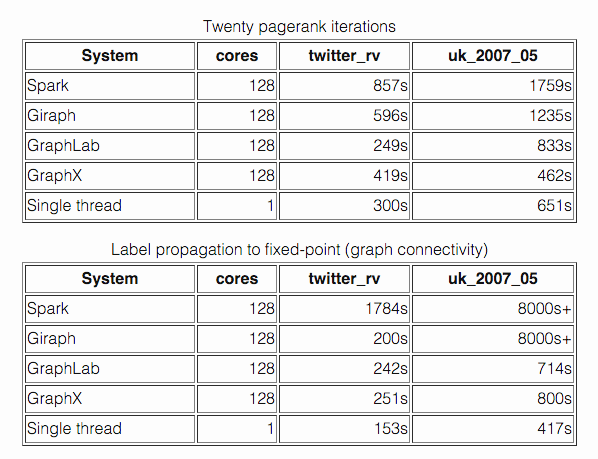
\includegraphics[width=0.60\textwidth]{images/pagerank.png}
\end{center}

\paragraph{Wait, there's more.} I keep on saying that we can improve algorithms for additional performance boosts too.
But that doesn't generalize, so it's hard to teach. In this case, two improvements are: using Hilbert curves
for data layout, improving memory locality, which helps a lot for PageRank; and using a union-find algorithm 
(which is also parallelizable). ``10$\times$ faster, 100$\times$ less embarrassing''.  We observe an overall
$2\times$ speedup for PageRank and $10\times$ speedup for label propagation.

\paragraph{Takeaways.} Some thoughts to keep in mind, from the authors:
\begin{itemize}
\item    ``If you are going to use a big data system for yourself, see if it is faster than your laptop.''
\item    ``If you are going to build a big data system for others, see that it is faster than my laptop.''
\end{itemize}



\section*{Movie Hour}
Let's take a humorous look at cloud computing: James Mickens' session from Monitorama PDX 2014. 

\begin{center}
\url{https://vimeo.com/95066828}
\end{center}









\chapter*{31 --- Introduction to Queueing Theory}

\addcontentsline{toc}{chapter}{31 --- Introduction to Queueing Theory}

\section*{A Short Introduction to Queueing Theory}

Queueing theory is literally the theory of queues---what makes queues appear, how will they behave, and how do we make them go away? Queueing theory has played a role in your life whether you know it or not: this is how tech support at Rogers or Bell or Telus or whomever decides just how many customer service agents to have available at any given time. Of course, your local telecom chooses to minimize the number of employees at the cost of making you wait (``Your call is important to us; please hold while we ignore it.'') but they study carefully how much waiting is too much waiting and how much is too little. Queueing theory is applicable to lots of fields, including industrial design, call centres, telecom systems, and computers executing transactions. 

To scale up a system, we have a lot of choices to make, and these will work best if they are supported by data. Queueing theory helps us decide what's best. Here are a few possible examples, from~\cite{pmd}:

\begin{itemize}
 \item Given a choice between a single machine with speed $s$ or $n$ machines, each with speed $s/n$, which should we choose?
 \item If the arrival rate and service rate double, how does the mean response time change?
 \item Should we try to balance load or is that a waste of time/effort?
 \item Can we give priority to certain operations without harming another category of job?
 \item How do job size variability and heavy-tailed workloads affect our choices of scheduling policy?
 \item If 12 servers is enough to handle 9 jobs per second, do we need 12~000 servers if we have an arrival rate if 9~000 jobs per second?
\end{itemize}

I tend to tell stories about banks that imply I hate them. Not really, they're just a place where there's likely to be a queue and I'm likely to be annoyed and thinking about how to optimize this situation. So let's define some terms formally, to make sure we're all on the same page when it comes to terminology and language. Some of these will seem obvious, but let's be complete (like the book~\cite{swps}):

\begin{itemize}
	\item Server - The banking centre fulfilling customer requests.
	\item Customer - Initiator of service requests.
	\item Wait time - The time a customer spends waiting in line.
	\item Service time - The time from when a teller starts to serve a customer up to the time when the next customer is called forward.
	\item Arrival rate - The rate at which customers arrive.
	\item Service rate - the rate at which customer requests are serviced.
	\item Utilization - The fraction of the teller's time used actually handling customer requests (not idling).
	\item Queue length - The total number of customers waiting, or currently with a teller, or both.
	\item Response time - The sum of wait and service time for a single visit.
	\item Residence time - The total response time if a customer visits several tellers (or the same one multiple times).
	\item Throughput - The rate at which customers get their requests serviced and dealt with.
\end{itemize}

The mathematical symbols for this are represented in the following table~\cite{swps}:


\begin{center}
	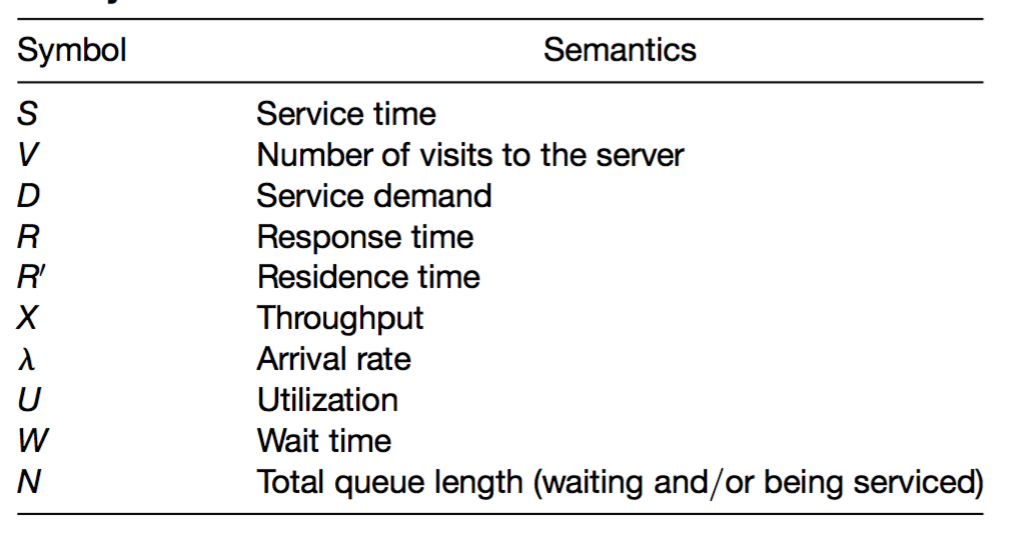
\includegraphics[width=0.65\textwidth]{images/math-symbols.png}
\end{center}

If you're cynical like me, you will think the bank works very hard to not have tellers in the bank to maximize your wait time and minimize their staffing costs. It's actually (allegedly) a trade-off: if I have to wait too long to do my banking, I could always take my business elsewhere (but is that likely to happen?). Minimizing customer wait time makes customers happy, so that's something the bank should want. It would also be nice if the bank trains its tellers well, so they can complete all operations, even unusual ones, quickly and efficiently, reducing the service time. The bank is not a charity operation so they will of course want to minimize staffing, but it knows that overstaffed is bad and understaffed is also bad. 

Back to the realm of computers: you have lots of queues in your computer. The CPU uses a time-sharing scheduler to run as many concurrent programs as possible. A router has a queue for packets (data) that has a maximum size, and if this is exceeded, packets will be simply dropped. 

Queueing theory gives us a formal framework with which to grapple with our problems instead of just guessing. Remember how bad we are at guessing. 


\paragraph{Example.} Let's look at a simple example from~\cite{pmd}. Imagine we have a system with one CPU that serves a queue of jobs in First-Come-First-Served (FCFS) order with an arrival rate $\lambda$ of 3 jobs per second. Each job takes some amount of time and resources, but we can ignore the particulars for right now. Suppose the average service rate $\mu$ is 5 jobs per second (or stated another way, the average job requires $0.2s$ to service). The system is not overloaded: 3 jobs per second arriving is less than 5 jobs per second being serviced. Our terminology for describing the mean response time will be $E[T]$. 


Suppose now that your boss says that tomorrow the arrival rate will double. If you do nothing, you can imagine, there will be a problem: we would have 6 jobs arriving per second, on average, to a system that can service, on average, 5 jobs per second. You have been allocated some budget to replace the CPU with a faster one, and you should choose one so that the jobs still have a mean response time of $E[T]$. This situation is depicted below~\cite{pmd}:


\begin{center}
	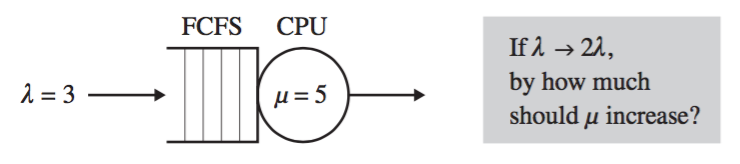
\includegraphics[width=0.5\textwidth]{images/qt-example1.png}
\end{center}

That is, customers should not notice the increase in arrival rate. So, should we (1) double the CPU speed; (2) more than double the CPU speed; or (3) less than double the CPU speed?

The answer is (3): we don't need to double the CPU speed. We can see later in formal terms why this is the case, but think for a minute about why it is? If we double the service rate and double the arrival rate, we actually get half the mean response time...

\paragraph{Example 2.} Okay, how about another example from~\cite{pmd}. There are always $N=6$ jobs running at a time. As soon as a job completes, a new one is started (this is called a \textit{closed system}). Each job goes through to be processed on one of two servers (and it is 50-50 where the job ends up), each of which has a service time $\mu$ of 1 job per 3 seconds. Again, depicted below~\cite{pmd}:


\begin{center}
	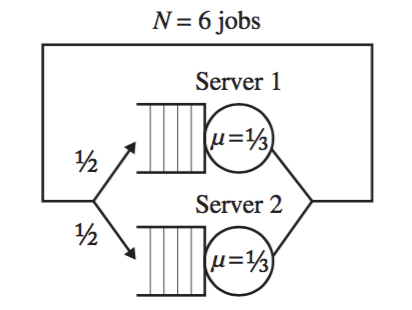
\includegraphics[width=0.3\textwidth]{images/qt-example2.png}
\end{center}

Bad news: sometimes, improvements do nothing. If we replace server 1 with one which is twice as fast (so 2 jobs per 3 seconds), does that help? Nope. Not really. Does raising $N$ help? Nope, negligible effect. The bottleneck device is the limiting factor. Strangely, dropping $N$ to 1 means the server replacement makes a difference, if you can call that improvement. 

What if it's an \textit{open system} where arrival times are independent of completion, as below~\cite{pmd}?


\begin{center}
	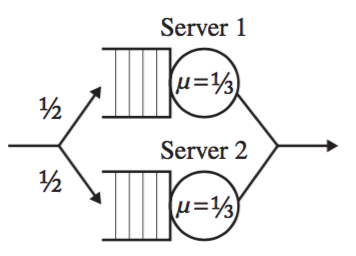
\includegraphics[width=0.3\textwidth]{images/qt-example2-2.png}
\end{center}

In this case, yes, replacing server 1 makes a huge difference!

\paragraph{Example 3.} A third example, this time addressing directly the question of do we want one fast server or $n$ slower ones? Horse-sized duck and duck-sized horses jokes aside, what is better if we want to minimize the mean response time when we have non-preemptable jobs (i.e., once started, a job has to run to completion and cannot be interrupted)~\cite{pmd}:


\begin{center}
	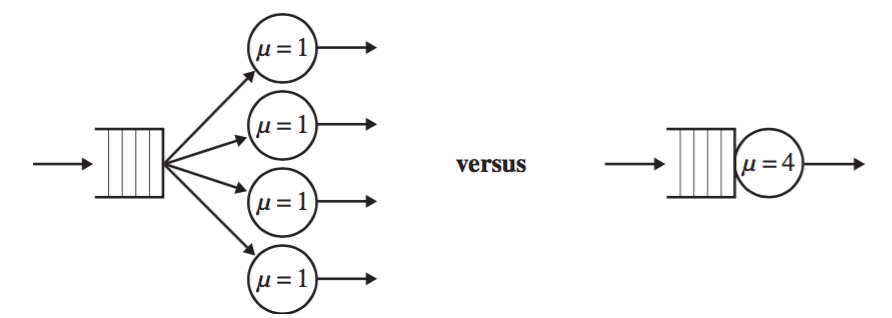
\includegraphics[width=0.6\textwidth]{images/qt-example3.png}
\end{center}

The answer is ``it depends''. That's frustrating, but this is Sparta. Or at least, real life. One big factor is the variability of the job sizes. Imagine you are at the grocery store and most people have 12 items or fewer\footnote{Not less. Fewer. It is countable; therefore fewer. Yes, I am obsessive about this.} and there's one guy who's buying 85 items. You don't want to be standing in line with milk and eggs behind someone who is trying to buy six of everything, do you? So if there's high variability, you probably want multiple servers---the guy buying the whole store can hold up line \#1 and you can go to line \#4 and you're out and done before he is finished.

What if the load is low? Chances are you would prefer the one fast server instead of having some number of servers doing nothing.

What if jobs are interruptible (preemptible)? You could always use a single fast machine to simulate $n$ slow machines, so a single fast machine is at least as good as the alternative. 

\subsection*{A Digression on Load Balancing}

Imagine your typical ``server farm''---you have $n$ servers that are all responsible for handling incoming requests. Let's imagine all servers are the same (or close enough). What we typically see in load balancing is assignment of tasks to servers via some dispatcher~\cite{pmd}:

\begin{center}
	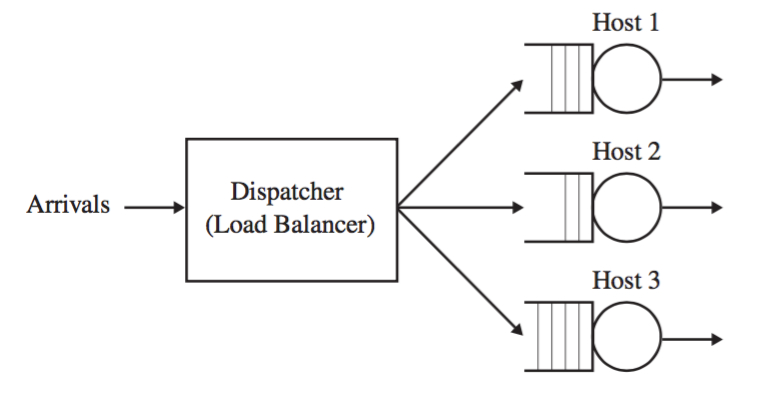
\includegraphics[width=0.6\textwidth]{images/central-dispatcher.png}
\end{center}

This isn't the only kind of load balancing we can do; there is also the ability to do after-the-fact assignment (or work-stealing), which consists of monitoring the various queues and reassigning work if it's piling up somewhere.

There are a few different task assignment policies---ways in which we can assign work to servers~\cite{pmd}:

\begin{itemize}
	\item Random: Exactly what it sounds like.
	\item Round-Robin: The $i$th job goes to host $i$ modulo $n$.
	\item Shortest-Queue: The job goes to the server with the shortest queue.
	\item Size-Interval-Task-Assignment: Short jobs go to one server, medium to another, long to another...
	\item Least-Work-Left: A job goes to the server that has the least total remaining work, where work is the sum of the size of the jobs.
	\item Central-Queue: Rather than being assigned to a host directly, when a server needs work to do, it gets the first job in the central queue.
\end{itemize}

Which of these policies yields the lowest mean response time? Answer: truthfully, nobody knows. It depends, of course, on your job variability and and that sort of thing, but it hasn't been well studied. PhD, anyone?

\subsection*{Red Line Overload\footnote{You've seen ``Top Gun'', right? \url{https://www.youtube.com/watch?v=siwpn14IE7E}}}

Earlier I mentioned it would probably be bad to see 6 jobs arriving per second to a system that can handle 5 per second. This doesn't seem like rocket science, but it bears repeating. In our discussion we require that $\lambda \leq \mu$ and assume that $\lambda < \mu$. That is to say, we are not overloaded (as engineering students you may be amused by the idea that you might one day NOT be overloaded). Remember now that the values for $\lambda$ and $\mu$ are averages, so it could happen that temporarily we ``fall behind'' a bit, but then make up for it a little later on, or we temporarily get ahead before a bunch more work gets piled on. Think about the long term, though -- if we are not at least keeping up then this will eventually get out of hand. How badly? Well, in the limit, the queue length goes to infinity.

The justification comes from~\cite{pmd}: Let's represent time with $t$, its usual symbol and define $N(t)$ as the number of jobs in the system at time $t$. $A(t)$ represents arrivals by time $t$ and $D(t)$ represents departures by time $t$. So:

\begin{center}
	$E[N(t)] = E[A(t)] - E[D(t)] \geq \lambda t - \mu t = t (\lambda - \mu) $
\end{center}

The tiniest bit of calculus says that if arrivals exceed departures, taking the limit as $t$ goes to infinity means $t (\lambda - \mu) $ also goes to infinity. Whoops. So to prevent this terrible situation we just happily assume that this doesn't happen\footnote{I'm reminded of a funny engineering saying that says if you encounter a system that is nonlinear, you can decide that nonlinear systems are too difficult to reason about, assume the system is linear, and proceed.}. 

Raising $\mu$ is generally desirable. This is, after all, programming for performance -- the faster we complete work, the more work we can get done in the same amount of time. Improving the service rate, however, does not necessarily improve the throughput. 

Wait, what? We've assumed that the arrival rate is less than the service rate. So we have enough capacity to handle all incoming work. So the limiting factor on completed work is actually arriving work. We have the capacity to do at least what is arriving and possibly a bit more. Adding more work capacity doesn't mean more work gets done if there isn't any more work to do. You might be capable of completing six assignments for this class in a term, but if you're (mercifully) only assigned four, then you will only complete four. So raising $\mu$ increases the maximum possible throughput, but does not necessarily increase the actual throughput.

But just to make you suffer, things are very different in a closed system: one in which there is always more work to do and as soon as one item is finished the next one enters the queue. This is the case in batch systems. You know, the old mainframe kind of processing where you submit your job to be run overnight and in the morning you get a result. Hopefully the one you wanted. In that case, we are running at capacity all the time, so actually $\mu$ is the controlling factor -- the throughput is exactly the service rate. 

Not that open networks are particularly intuitive, but closed networks can kind of mess with our intuition in general. Imagine we have a closed system with Multiprogramming Level (MPL) of $N$ as below~\cite{pmd}:

\begin{center}
	\includegraphics[width=0.4\textwidth]{images/tandem-closed.png}
\end{center}

What is the throughput here? Intuition suggests min($\mu_{1}, \mu_{2}$), right? Sometimes. This is okay if the slower server is always busy, but that's not always the case. What if $N$ is 1? Okay, that's a bit of an exception case though. What about $N$ being 2? Then the slower server has some work to do at all times right? Nope, sadly not. Sometimes the slow server is faster than the fast server, because $\mu_{1}$ and $\mu_{2}$ are just averages. And averages can be misleading! The average family might have 2.3 children (or whatever the figure is), but you can't exactly have 0.3 of a child...

\subsection*{Don't Guess...}
One final anecdote from~\cite{pmd} on the subject of measuring $\mu$. Some smart folks at IBM wanted to know, given the arrival rate $\lambda$, what the mean job size, $E[S]$ (which is $1/\mu$) was. Well, $E[S]$ is the mean time required for a job in isolation, so our experiment should be a hundred runs of sending a single job into the system and averaging the values. This is okay, but does not reflect reality where we have things like caching of data and multiple concurrent jobs. There are two basic strategies we can follow for getting a value for $\mu$ (depending on whether it is an open or closed system), allowing simple computation of $E[S]$.

The open system strategy is: ramp up $\lambda$. Keep piling more jobs on the system. At some point the system will not be able to keep up. Once the completion rate levels off, we hit the limit and we have a value for $\mu$.

The closed system strategy: set it up so there is always work to do. In closed systems, there's often consideration given to \textit{think time}---this is what happens when the user is on the command line and dispatching work to do. The user sends a command and awaits a result. After the result, some time passes while the user decides what to do next (or does code editing before running the compiler again). To keep the system totally busy in the stress test, we need think time to be zero---so additional work is always available. And then we can simply measure the jobs completing per second, giving us $\mu$ directly.




practical queueing theory:  https://www.youtube.com/watch?v=IPxBKxU8GIQ





\chapter*{32 --- Convergence, Ergodicity, Applications}

\addcontentsline{toc}{chapter}{32 --- Convergence, Ergodicity, Applications}

\section*{Convergence}

Think back to calculus class. Remember when we talk about limits: $\lim_{x\to\infty} f(x)$. There is an answer for this if the function does (somehow) converge on some value, such as the function $f(x) = 1/x^{2}$ converging to 0.

We would like to see that our random variables converge. You might flip a coin four times and all four times it comes up heads. That doesn't match our expectation that we should have about half heads and half tails. We have convergence if, given enough samples and enough sample paths, it will converge to the 0.5 we expect. There may be some sample paths that don't converge (e.g., continually coming up heads), but they have a ``probability mass'' of zero (i.e., they are incredibly unlikely).  There are in fact uncountably many ``bad paths'', each with probability zero (but that's okay). Zero probability doesn't mean it can't happen, mind you.

An image of what convergence looks like~\cite{pmd}:

\begin{center}
	\includegraphics[width=0.6\textwidth]{images/convergence.png}
\end{center}

We won't concern ourselves with systems where there is no convergence. We'll just deal with situations where there is a convergence. Almost every sample path (series of experiments) will eventually behave well if we take enough samples. That is, get past the initial conditions. But sampling is important in our discussion about scalability...

\section*{Tim and Enzo}
A small but important digression on the subject of sampling, measurement, and testing, from~\cite{pmd}. You have an idea of what an average is, but there are two different relevant types of average here---the time average and ensemble average. 

Let us just focus on having a single First-Come-First-Serve queue. Every second, a new job arrives with probability $p$ and if there is any work to do, the job being worked on is completed with probability $q$ (and $q > p$). As a definition, let $N(v)$ equal the number of jobs in the system at a time $v$. In the story, Tim and Enzo are trying to simulate the FCFS system to determine what is the average number of jobs in the system. 

Tim decides he's going to run it as one really long simulation. He simulates the queue over a very long period, logging as he goes, taking a million samples. Then he takes the average value over those samples to get the average number of jobs.

Enzo does something slightly different: instead of having one super long simulation, he does 1000 shorter simulations. He waits until the simulation has run for 1000 seconds and then samples the queue at exactly that point, obtaining one value. This experiment is restarted with a new random seed. So after obtaining a thousand samples, he averages these, and Enzo produces another average number of jobs.

A little illustration of Tim and Enzo from~\cite{pmd}:

\begin{center}
	\includegraphics[width=0.5\textwidth]{images/timenzo.png}
\end{center}

So -- who has done this correctly, Tim or Enzo?

The time average has potential problems because we are only looking at a single sequence and maybe something very unusual has happened here in this single run. The ensemble average is more likely what we talk about when we talk about the system being at ``steady state'' (i.e., past the initial conditions). So we kind of like the Enzo approach. Plus, this is programming for performance (or as a student said, programming for parallelism) -- we can do 1000 simulations concurrently if we have enough CPU cores! Tim's approach still has some merit though.

A note about initial conditions: both the Tim and Enzo approaches here require caring about the initial conditions. Enzo needs to make sure that the initial conditions (startup costs etc) have attenuated before the measurement point. Tim needs to ensure that the initial conditions impact a sufficiently small portion of all his measurements.

But! If we have a nicely behaved system, the time average and the ensemble average are the same (so both Tim and Enzo can be correct). What is a nicely behaved system? The word for this is \textit{ergodic}. That probably did not help, so what is an ergodic system? It is a system that is positive recurrent, aperiodic, and irreducible.

\textit{Irreducibility} means a process should be able to get from one state to any other state (where state is the number of jobs in the system). This means the initial state of the system does not matter. So if we started at 0 jobs or 10 we could still get to any state in the system (jobs at 2 or 27)\ldots

\textit{Positive recurrence} means that given an irreducible system, any state $i$ is revisited infinitely often, and the time between visits to that state are finite. So we can define a certain state as being a ``restart''. The logical choice in the case of a queue or similar is the idea of the queue being empty. Every time the queue gets down to zero jobs, it's a ``restart'' of sorts. 

This is what makes Tim's view and Enzo's view potentially the same. A single long run (Tim's view) is just like a number of independent runs (Enzo's view). Every time we get down to zero jobs in the queue, it's a restart. 

The \textit{aperiodicity} condition is required for the ensemble average to make sense or exist. That is to say, the state of the system should not be related to the time; i.e., it is not the case that the system is in state 0 when $t$ is even and state 1 when $t$ is odd. Otherwise the way Enzo chooses to sample, i.e., $t = 1000$, is potentially going to skew the result.

A graphical illustration, also from~\cite{pmd}, that shows how the time average over a single long run can be considered a chain of restarts or ``renewals''.

\begin{center}
	\includegraphics[width=0.5\textwidth]{images/systemrestart.png}
\end{center}

Both Tim and Enzo are correct for ergodic systems. Either method works to determine measurements and queueing theory values. Enzo's method has some advantages, e.g. parallelism and the ability to produce confidence intervals.

We've talked about the average number of jobs, but perhaps what we also care about is how long a job spends in the system, on average. We could compute either the time or ensemble average. 

\begin{center}
	Time Average = $\lim_{t\to\infty}\dfrac{\sum_{i=1}^{A(t)} T_{i}}{A(t)},$
\end{center}

where $A(t)$ is the number of arrivals by time $t$ and $T_{i}$ is the time in the system of arrival $i$. The average is taken over one sample path.

\begin{center}
	Ensemble Average = $\lim_{t\to\infty}E[T_{i}],$
\end{center}

where $E[T_{i}]$ is the average time in the system of job $i$, average being taken over all sample paths.

\section*{Little's Law}
Little's Law is a famous result, saying that the average number of jobs in the system equals the product of the average arrival rate into the system and the average time spent in the system. The source on this section is~\cite{pmd}.

\paragraph{Open Systems.} Let's start with an open system. Here is Little's Law, written more formally:

\[
	E[N] = \lambda E[T],
\]

where $E[N]$ is the expected value of the number of jobs in the system, $\lambda$ is the average arrival rate into the system, and $E[T]$ is the mean time jobs spend in the system. For example, if a University intakes an average of 5,000 students per year and each student spends an average of 4 years in school, then there are $4 \times 5000=20000$ students on average in the University~\cite{sigman-little-law}. The basic setup of Little's Law looks something like this~\cite{pmd}:

\begin{center}
	\includegraphics[width=0.5\textwidth]{images/littleslaw.png}
\end{center}

We don't need to know anything about the arrival process (Bernoulli, Poisson, etc\ldots), the service time distribution, network topology, etc. It seems intuitive that this is the case (or it should). Imagine a fast food restaurant: they make money by quick turnaround, so they get people out of the place quickly (low $E[T]$) and accordingly they don't require a lot of seating (low $E[N]$). A sit down restaurant is the opposite though; people leave slowly (high $E[T]$) and therefore the restaurant needs lots of seating (more $E[N]$). This example might seem weird from the perspective of the customer though---from your perspective, you may want to enjoy your evening---but the restaurant is eager to turn your table over, and get you out of there so a new set of guests can be seated. (Another way of looking at this is that restaurants are in the business of renting seats. It's not about food costs.)

If you prefer to think of this in a single FCFS queue version, imagine a customer arrives and sees $E[N]$ jobs ahead of her in the queue. The expected time for each customer to complete is $1/\lambda$, because the average rate of completions is $\lambda $. So we can approximate $E[T]$ as being roughly $\dfrac{1}{\lambda}E[N]$.

\paragraph{Closed Systems.} Remember that for closed systems, we have a rule that says there are $N$ jobs in process at any given time (the multiprocessing level of the system). If the system is ergodic, then $N = X \cdot E[T]$ where $N$ is the multiprogramming level, $X$ is the throughput rate, and $E[T]$ is the mean time jobs spend in the system. This assumes that there is zero think time, i.e., that jobs are always ready at once and don't have to wait for silly users.

If we do have to deal with the vagaries of users and think time, then we care more about the response time $E[R]$. So for a terminal-driven system, the expected response time is $E[R] = \dfrac{N}{X} - E[Z]$ where $N$ is the multiprogramming level, $X$ is the throughput, and $E[Z]$ is the mean time spent thinking. 

\section*{M/M/1}

Probabilistic processes are described according to their models, which will probably be one of the three~\cite{swps}:

\begin{enumerate}
	\item Deterministic (D) -- The process is predictable and characterized by constant factors. For example, the inter arrival times are constant (e.g., a task arrives every minute.)
	\item Markov (M) -- A memoryless process; the future states of the process are independent of the past history. The future state depends on only the present state.
	\item General (G) -- Completely arbitrary.
\end{enumerate}

We're going to focus on Markov processes, because they are nicer (and we have only limited time). It means that the number of arrivals follow the Poisson distribution; the inter-arrival times follow the exponential distribution, and service times follow the exponential distribution too. 

Those letters we saw are part of Kendall notation. It has six symbols, written in a specific order, separated by slashes. The order is $\alpha / \sigma / m / \beta / N / Q$. See the table below for the full explanation:

\begin{center}
\begin{tabular}{l|l} 
	\textbf{Symbol} & \textbf{Meaning} \\ \hline
	$\alpha$ & The type of distribution (Markov, General, Deterministic) \\ \hline
	$\sigma$ & The type of probability distribution for service time \\ \hline
	$m$ & Number of servers \\ \hline
	$\beta$ & Buffer size \\ \hline
	$N$ & Allowed population size (finite or infinite) \\ \hline
	$Q$ & Queueing policy \\ 
\end{tabular}
\end{center}

We often leave off the last three, assuming that there is an infinite buffer, infinite population, and a FIFO queueing policy. If that is the case, then we have only three values. Those three then produce the ``M/M/1'' and ``M/M/k'' symbols. ``M/M/1'' means a Markov arrival process, exponential queueing system, and a single server. When there are $k$ servers, of course the 1 is replaced with the $k$. These are the systems that we are going to examine.

We should also think about utilization, denoted $\rho$. It is a fraction between 0 and 1 and it is simply the amount of time that the server is busy. We talked about this earlier in an informal way, but now we can actually calculate it: $\rho = \lambda \times s$ (the arrival rate and service time). 

For M/M/1 systems, the completion time average $T_{q}$ is $\dfrac{s}{(1-\rho)}$ and the average length of the queue $W$ is $\dfrac{\rho^{2}}{1-\rho}$.

An example from~\cite{williams-q}: we have a server that completes a request, on average, in 10~ms. The time to complete a request is exponentially distributed. Over a period of 30 minutes, 117~000 jobs arrive. So this is a M/M/1 situation. How long did it take to complete the average request? What is the average length of the queue?

The service time $s$ is given as $0.01s$ and the arrival rate is 65 requests per second. So we can calculate $\rho = 0.01 \times 65 = 0.65$. So we have what we need to plug and chug using the formul\ae\ from above to find the time to complete the average request is 28.6~ms and the average length of the queue is 1.21.

What about the number of jobs in the system? The value $\rho/(1 ? \rho)$ gives the average number of jobs, including the waiting jobs and the ones being served. It is an average, of course. The probability that there are exactly $x$ jobs in the system at any time is given by the formula: $(1-\rho)\rho^{x}$. The probability that the number of jobs is less than or equal to $n$ is then given by: $\sum\limits_{i=0}^{n}(1-\rho)\rho^{i}$ (the sum of the probabilities of each of the numbers from 0 up to $n$). If you want to know the probability that there are more then $n$ at a time, then you can compute the sum from $n+1$ up to infinity. That might be unpleasant to calculate, but remember that probabilities sum to 1, so you can say that the probability of more than $n$ requests at once is simply $1 - \sum\limits_{i=0}^{n}(1-\rho)\rho^{i}$.

\section*{M/M/k}

Now let us take it to multiple servers ($k$ of them, in fact). We will say jobs arrive at a single queue and then when a server is ready it will take the first job from the front of the queue. The servers are identical and jobs can be served by any server. So far, so simple.

Sadly, the math just got harder. Let's turn again to~\cite{williams-q} as the source for this section. The server utilization for the server farm is now $\rho = \lambda s / N$ (the average utilization for all $N$ servers). To make our calculations a little easier, we want an intermediate value $K$ which looks scary, but is not so bad:

\[ K = \cfrac{\sum_{i=0}^{N-1}\dfrac{(\lambda s)^{i}}{i!}}{{\sum_{i=0}^{N}\dfrac{(\lambda s)^{i}}{i!}}}.
\]

The first term, $i = 0$, is always 1. The denominator is always larger than the numerator, so $K$ is always less than 1. $K$ has no intrinsic meaning, it is just a a computational shorthand so the other formul\ae\  are not so messy.

What is the probability that all servers are busy? We represent this as $C$, the probability a new job will have to wait in the queue.

\[C = \cfrac{1 - K}{1 - \dfrac{\lambda s K}{N}}.\]

The M/M/k formul\ae, then, for the average completion time and average length of the queue are:

\[
  T_{q} = \dfrac{C s}{k(1 - \rho)} + s \mbox{ \qquad\qquad and \qquad\qquad } W = C \dfrac{\rho}{1 - \rho}.
\]

Let's do an example. Suppose we have a printer that can complete an average print job in two minutes. Every 2.5 minutes, a user submits a job to the printer. How long does it take to get the print job on average? We're starting with a single printer, so the system is M/M/1. Service time $s$ is 2 minutes; the arrival rate $\lambda$ is $1/2.5 = 0.4$. So $\rho = \lambda \times s = 0.4 \times 2 = 0.8$. So $T_{q} = s / (1 - \rho ) = 2 / (1 -0.8 ) = 10$. Ten minutes to get the print job. Ouch.

Here we have an opportunity to use the predictive power of queueing theory. Management is convinced that ten minute waits for print jobs is unreasonable, so we have been asked to decide what to do: should we buy a second printer of the same speed, or should we sell the old one and buy a printer that is double the speed?

The faster printer calculation is easy enough. Now $s = 1.0$ and $\lambda$ remains $0.4$, making $\rho = 0.4$. So rerunning the calculation: $T_{q} = s / (1 - \rho ) = 1 / (1 - 0.4 ) = 1.67$. 1:40 is a lot less time than 10:00! 

The two printer solution is more complicated. So let us calculate $K$ as the intermediate value. 

\[K = \cfrac{\sum_{i=0}^{N-1}\dfrac{(\lambda s)^{i}}{i!}}{{\sum_{i=0}^{N}\dfrac{(\lambda s)^{i}}{i!}}} = \cfrac{\dfrac{(\lambda s)^{0}}{0!} + \dfrac{(\lambda s)^{1}}{1!}}{\dfrac{(\lambda s)^{0}}{0!} + \dfrac{(\lambda s)^{1}}{1!} + \dfrac{(\lambda s)^{2}}{2!}} = 0.849057.\]

Now we can calculate $C$ as 0.22857 and $T_{q}$ as 2.38 minutes (by simple plug and chug calculations given the formul\ae\  above). Two observations jump out at us: (1) we doubled the number of printers, but now jobs are completed almost four times faster; and (2) the single fast printer is better, if utilization is low.

That is an important condition: if utilization is low. At some point will the two printers be a better choice than the single fast one? What if both printers are used to the max (100\% load)\ldots?

\section*{Queuing for Performance}

The plan is to take queueing theory and apply it in a performance model. The guide to this section is~\cite{williams-perf}. The basic process is:

\begin{enumerate}[noitemsep]
	\item Convert to common time units.
	\item Calculate the visitation ratios $V_{i}$.
	\item Calculate the device utilization $\rho_{i}$.
	\item Calculate the CPU service time.
	\item Calculate the device time.
	\item Find the bottleneck device.
	\item Calculate the maximum transaction rate.
	\item Calculate the average transaction time.
\end{enumerate}

Let us execute this process on a web server system that serves 9~000 pages per hour. Here are the known values:

\begin{center}
\begin{tabular}{l|r|r|r|r|r|r} 
	\textbf{Device} & \textbf{Data/Hour} & \textbf{$\lambda$} & \textbf{$S$} & \textbf{$V$} & \textbf{$\rho$} & \textbf{$V \times S$} \\ \hline
	Webpages & 9~000 & & & & & \\ \hline
	CPU & & & & &  42\% & \\ \hline
	Disk 1 & 108~000 & & 11ms & & &\\ \hline
	Disk 2 & 72~000 & & 16ms & & &\\ \hline
	Network & 18~000 & & 23ms & & &
\end{tabular}
\end{center}

Step one is to convert to common time units; in this case, seconds. That would be a simple and common time unit. Let's also look at the $\lambda$ values - reported counts divided by seconds in the reporting period.

\begin{center}
\begin{tabular}{l|r|r|r|r|r|r} 
	\textbf{Device} & \textbf{Data/Hour} & \textbf{$\lambda$} & \textbf{$S$} & \textbf{$V$} & \textbf{$\rho$} & \textbf{$V \times S$} \\ \hline
	Webpages & 9~000 & 2.5 & & & & \\ \hline
	CPU & & & & & 42\% & \\ \hline
	Disk 1 & 108~000 & 30 & 0.011s  & & &\\ \hline
	Disk 2 & 72~000 & 20 & 0.016s & & &\\ \hline
	Network & 18~000 & 5 & 0.023s & & &
\end{tabular}
\end{center}

The visitation ratio is the number of times a device is used in each transaction; divide use by number of transactions to get $V_{i}$ (you could also log this sort of thing). The visitation ratio of the CPU is the sum of all other visitation ratios. Why? Suppose we do a disk read: the disk is visited, and when the disk read completes, we go back to the CPU and it picks up the data that's just been shuttled in from the impossibly slow disk.

\begin{center}
\begin{tabular}{l|r|r|r|r|r|r} 
	\textbf{Device} & \textbf{Data/Hour} & \textbf{$\lambda$} & \textbf{$S$} & \textbf{$V$} & \textbf{$\rho$} & \textbf{$V \times S$} \\ \hline
	Webpages & 9~000 & 2.5 & & 1 & & \\ \hline
	CPU & 207~000 & 57.5 &  & 23 & 42\% & \\ \hline
	Disk 1 & 108~000 & 30 & 0.011s  & 12& &\\ \hline
	Disk 2 & 72~000 & 20 & 0.016s & 8 & &\\ \hline
	Network & 18~000 & 5 & 0.023s & 2 & &
\end{tabular}
\end{center}

Next, calculate device utilization: $\rho = \lambda \times s$. That is, arrival rate times service time.

\begin{center}
\begin{tabular}{l|r|r|r|r|r|r} 
	\textbf{Device} & \textbf{Data/Hour} & \textbf{$\lambda$} & \textbf{$S$} & \textbf{$V$} & \textbf{$\rho$} & \textbf{$V \times S$} \\ \hline
	Webpages & 9~000 & 2.5 & & 1 & & \\ \hline
	CPU & 207~000 & 57.5 &  & 23 & 0.42 & \\ \hline
	Disk 1 & 108~000 & 30 & 0.011s  & 12& 0.33 &\\ \hline
	Disk 2 & 72~000 & 20 & 0.016s & 8 & 0.32 &\\ \hline
	Network & 18~000 & 5 & 0.023s & 2 & 0.115 &
\end{tabular}
\end{center}

A small oddity: in the CPU we have a percentage for utilization rather than a decimal number. Just convert it to 0.42. And we can also get the service time of the CPU by rearrangement of the utilization formula to $s = \rho / \lambda$.

\begin{center}
\begin{tabular}{l|r|r|r|r|r|r} 
	\textbf{Device} & \textbf{Data/Hour} & \textbf{$\lambda$} & \textbf{$S$} & \textbf{$V$} & \textbf{$\rho$} & \textbf{$V \times S$} \\ \hline
	Webpages & 9~000 & 2.5 & & 1 & & \\ \hline
	CPU & 207~000 & 57.5 & 0.0073s & 23 & 0.42 & \\ \hline
	Disk 1 & 108~000 & 30 & 0.011s  & 12& 0.33 &\\ \hline
	Disk 2 & 72~000 & 20 & 0.016s & 8 & 0.32 &\\ \hline
	Network & 18~000 & 5 & 0.023s & 2 & 0.115 &
\end{tabular}
\end{center}

And the device time is the final thing we can fill in for this table: $V_{i} \times S_{i}$ (just like the column header says!).

\begin{center}
\begin{tabular}{l|r|r|r|r|r|r}
	\textbf{Device} & \textbf{Data/Hour} & \textbf{$\lambda$} & \textbf{$S$} & \textbf{$V$} & \textbf{$\rho$} & \textbf{$V \times S$} \\ \hline
	Webpages & 9~000 & 2.5 & & 1 & & \\ \hline
	CPU & 207~000 & 57.5 & 0.0073s & 23 & 0.42 & 0.168\\ \hline
	Disk 1 & 108~000 & 30 & 0.011s  & 12& 0.33 & 0.132\\ \hline
	Disk 2 & 72~000 & 20 & 0.016s & 8 & 0.32 & 0.128\\ \hline
	Network & 18~000 & 5 & 0.023s & 2 & 0.115 & 0.046
\end{tabular}
\end{center}

Did we need to complete the whole table? Probably not. In a practical sense what we cared about the most was the $\rho$ column -- utilization. The bottleneck device, i.e., the one that limits our maximum throughput, is the one that is the busiest. Thus, the one with the largest utilization. This application appears to be CPU bound; it has the highest utilization at 42\%, well ahead of disk 1 and disk 2. 

Having identified the bottleneck device as the CPU, we can make a prediction about the maximum rate of transactions (web page requests) we can serve: $\dfrac{1}{S_{i}V_{i}}$ or in this example, 5.95. This is also called saturation. If $\lambda$ exceeds this saturation point, we will not be able to keep up with incoming requests.

With this table we can also calculate the average transaction time: it is the sum of the $S_{i}V_{i}$ columns. In this example, it is 0.474 seconds. 

\paragraph*{It Gets Worse}

The typical assumption is that we know the service times for each device. Unfortunately this is not true; usually performance monitoring gives us the average size of a device queue. So we had better apply queuing theory here, once again credit to~\cite{williams-calc} for the section. 

The average size of a device's queue is $W$, and for a queue with characteristics M/M/1 then $W = \dfrac{\rho^{2}}{1-\rho}$. Combining the known $W$ with the average arrival rate $\lambda$, we can work out the service time. $W = \dfrac{(\lambda s)^{2}}{1 - \lambda s}$, so:

\[ s = \cfrac{-w \pm \sqrt{w^{2}+4w}}{2\lambda}.\]

Yup. The quadratic formula strikes back. 








\newcommand{\FPP}{FastPass\nolinebreak\hspace{-.05em}\raisebox{.4ex}{\tiny\bf +}\nolinebreak\hspace{-.10em}\raisebox{.4ex}{\tiny\bf +}}
\def\FPP{{FastPass\nolinebreak[4]\hspace{-.05em}\raisebox{.4ex}{\tiny\bf ++}}}



\chapter*{33 --- More Advanced Queueing Theory}

\addcontentsline{toc}{chapter}{33 --- More Advanced Queueing Theory}

\section*{New Considerations}

There are a few new considerations, or, if you prefer, complications to queueing theory that we haven't yet covered in the fairly simple discussion of queueing theory we have had so far. But real life is considerably more complicated than a simple model. We'll talk about two settings, one that I love and one that I hate: food halls and Service Ontario. No points for guessing which is which.

If you're not familiar with them, a quick refresher. A food hall, or food court, is a place where there are a number of counter-service restaurants that frequently offer different cuisines. Service Ontario is a place of interaction with the administrative state, specifically the services administered by the provincial government of Ontario.

\paragraph{Multiple Services.} The way we have discussed the idea of services is that all the offered services are the same, or at the very least, every server can deliver every kind of service. That's sometimes reasonable -- at Service Ontario, there are many different services available (drivers license renewal, health card renewal, vehicle registration update, etc) and any one of the staff members there can help you with any one of those services.

There are, of course, other situations where an individual member of staff cannot provide all services and therefore you must queue for the specific thing that you want, even if the other queues are shorter or empty. A food hall works like this. The Mexican restaurant may be very popular because they have excellent tacos, resulting in a long queue for that particular place. There may be no queue at the Gelato stand, but that doesn't help; the Gelato place cannot provide tacos. And while both of these are food, you will probably agree that they're not (always) interchangeable. If you really want tacos, gelato won't do.

\paragraph{Maintenance, Planned and Otherwise.}
In real life, services will potentially have downtime, planned or otherwise, which can throw a wrench in things unexpectedly and sometimes that means closing the queue and sending requesters elsewhere. If the pizza place's oven breaks, they can't make any more pizza, and everyone in line for the pizza needs to go somewhere else if they want to eat today. We don't usually account for this directly when planning and designing our systems, possibly because we expect things to always be available and for people to be paged to fix it if it's not (see our next topic for more about this). But we might account for regular maintenance or planned downtime in our estimates of how many customers we can serve in a given period.

In principle, new services can also come online also. I don't mean more workers at Service Ontario, but more like what happens if a new restaurant opens. If new a Banh Mi place opens then people who are currently in line for a different food might prefer to switch because they like that cuisine better. In reality, like a restaurant opening, the presence of a new kind of service is rarely a true surprise: people have worked hard to build, test, and deploy it and it's not as though we just wake up one day and suddenly a new thing is just... there.

\paragraph{Interchangeability.} We already hit on the idea of interchangeability when talking about the food hall example. It's a spectrum: sometimes things are totally interchangeable, sometimes partly, and sometimes not at all. In the food hall example, total interchangeability is what happens if you're just extremely hungry and you would be completely happy whether you had tacos, pizza, or shawarma.  Partial interchangeability can happen when you have preferences but would accept something else: you want tacos but would choose shawarma under certain circumstances. And no interchangeability happens when you have your heart truly set on pizza and will accept nothing else.

Whether things are interchangeable depends on the nature of the services and the needs of the people requesting them. Just as there are different services in this more complicated world, requesters also behave differently.

All of the above food hall examples are about food, so there's at least a possibility of interchangeability because every option will have some nutritional value (in the sense of, it's edible food with calories in it; a nutritionist might say the gelato has no nutritional value because it's not a ``healthy'' choice). If you went to Service Ontario to renew your drivers' license, there are really no alternatives that get you the same result: a new health card just isn't the same thing.

Then there are the needs of the person requesting the thing:  If someone is a vegetarian, they might be okay with tacos or pizza, but not shawarma. If they are a vegan, maybe the only option for them is the taco stand, no matter how good the pizza place is or how long the line for tacos is.

\paragraph{Too Long.} 
While we're on the subject, when you're in the food hall and the length of a particular queue is too long, we may experience one of three behaviours: balking, reneging, or ``loss''. 

Balking is what happens when you look at the line and you decide it's too long and there's no point in even getting into the line. That's very common: if I want to go to Service Ontario and it's so busy that there is a long line out the door, I'm not going to bother. I'll come back another time (if I can -- sometimes it's important to do something before a deadline). In the food hall, if the queue for tacos is really long, I'll line up for the shawarma. 

Reneging is what happens if I enter the queue for tacos, but before I get to the front of the queue, I give up (leave the queue). If it's taking too long and I'm really hungry (or just impatient), this could happen. It could also happen if I'm at Service Ontario in between things (e.g., on a lunch break) and if time runs out I need to go back to work.

Loss is what happens when service is refused because of capacity limits. This comes from the idea of the early telephone systems, where there were $k$ circuits and if none of the $k$ circuits was free at the time a person wanted to make a call, that call was just dropped (that is, the call fails)~\cite{pmd}. That makes it a M/M/k/k system, in queueing theory notation. In the food hall or Service Ontario example, this is what happens if there's a capacity limit to the building and I'll be turned away by security if the building is full. I'm not allowed to queue up, no matter how badly I'd like to.

In both cases where I choose to leave, there's an implicit or explicit estimation of the waiting time provided. When I choose not to enter the queue at all, it's because I've looked at the queue length, and maybe done some assessment of the service time, and calculated that the wait time exceeds my willingness to wait. It's also possible that the establishment is kind enough to put out signs that say that the expected waiting time from this point is $X$ minutes. Not very common in a food hall or Service Ontario, but maybe the case in other places.

Obviously, my initial estimate can be wrong if I guessed incorrectly about the service time, or if the line is so long I can't see all of it and I don't get a good estimate. But another reason why my estimate might be wrong is if people can join the line ahead of me. Wait, what?

\paragraph{Priority.}
When I was last at Service Ontario, an elderly person with mobility restrictions showed up while I was waiting in line and that person was permitted to go to the front of the queue. It's sensible that priority would be given to this person -- asking them to stand in line a very long time is not nice. But of course, when they go into the line ahead of me, it increases my wait time. This increase may result in my decision to leave the line as the time has increased to the point that I can no longer, or at least no longer wish to, wait. 

Priorities for some groups over others are actually really interesting, because they have interesting effects and open up questions:

\begin{itemize}
	\item How much, if any, does giving priority to one group over another help the group being given priority?
	\item How much, if any, does giving priority to one group disadvantage the group not being given priority?
	\item Can the priority system incentivize people to choose things that are less popular?
	\item Recognizing that if everyone has priority, nobody has priority, how many requests can have priority before all benefit is lost?
\end{itemize}


\section*{Laboratory Study with a Mouse}

This section relies on a rather informative video by the channel Defunctland, about the history of the Disney Fastpass system~\cite{dldisney}. The actual video contains a lot of discussion about the history of Walt Disney World and other things that are not relevant here. But there are a few interesting things we can learn from it. In the video, there's a lot of background info but also some explanation of the simulation that was used to evaluate the situation.

Simulation? Yes -- at some point the queuing theory problem becomes so complex that our ability to reason about it and do the math with spreadsheets or Wolfram Alpha or hand calculations is a limiting factor. And a simulation allows us to validate our theories. But why is this system so complex that it requires a simulation?

If we abstract away some of the details of the Mouse and his friends, we're left with a system has many details that we need to concern ourselves with:

\begin{itemize}
	\item Every customer (requester) is an independent agent, which implies:
		\begin{itemize}
			\item They have different times of arrival at and departure from the park. With that said, most arrive early in the day and relatively few arrive later in the day
			\item They have different preferences of what they want to do while there
			\item They have different willingness to wait for the things they want to do
			\item They may or may not be willing to come back another day
		\end{itemize}
	\item The park has opening and closing times which implies:
		\begin{itemize}
		\item Requests cannot be submitted before opening time
		\item Requests cannot be submitted after closing time
		\item Requests submitted too close to closing time may not be served before closing
		\end{itemize}
	\item The park has different services that each have their own service rate and any of them could be down for maintenance (indepedently of any others)
	\item The services have a fixed maximum capacity: you cannot make more seats on the rides or run them faster to get more people through quicker
\end{itemize}

\paragraph{Relevance?}
An important observation here is that this model is fairly different from what we are used to talking about when thinking of servicing requests. When I go to Service Ontario, I want to renew my license as fast as possible and leave as fast as possible and hope not to return any time soon. If I am at the food hall, I may want to sample some number of different cuisines, but I'll eventually be full (or at least be unable to eat any more food) and then I'll leave. But in this model, the tourist goes to the Mouse Park and stays for some period of time, trying to do as much as you want to do. That doesn't sound like most of our software service scenarios. Is anything we're learning in this model applicable?

I'll argue yes. If I'm a person waiting in line for a specific ride, it's entirely irrelevant to me whether the 400 people in front of me have just arrived at the park, or if they've been here for hours and this is their tenth ride. Rides don't have to be completed in a specific order (in the sense that nothing bad happens if someone does them out of order).

You could just imagine that this model is functionally equivalent to one in which each person who goes on a ride immediately leaves the park, never to return, and is instantly replaced by another guest who has the same preferences about what to do. With more and more complex priority systems, this way of thinking about it might not hold up, but hopefully this argument is convincing.

\paragraph{User types.}
The simulation has a few different archetypes for the users that represent their different ``personalities'' based on the expected type of person who would attend the park. Some of them come frequently because they have an annual pass, so they can always come back another time if they prefer. Others are here today and today only and don't want to miss out. But without getting bogged down in the archetypes, the type of user decides (1) how long they will stay at the park, (2) when they will balk (what is their willingness to wait for a particular ride), and (3) what they want to do while they're here. The third point covers both their preferences of what rides they want to go on (in what priority sequence)  and if they want to do other things in the park (things that aren't rides).

\paragraph{Priority Systems.}
To establish a baseline, the simulation has an option where there's no priority system: everyone is equal. Then there are two different kinds of priority systems which the Mouse calls `FastPass'' and ``FastPass+'' (I'm sure the developers wanted to call it \FPP).

In the no-priority system, everyone is equal. Wait times are just based on how popular things are and nobody gets to cut in line. It helps wait times to be predictable, because the line a person in will advance at a fairly steady rate. No priority may seem fair at a glance, but is it optimal? Let's see. 

In the Fastpass system, instead of waiting in line, a person could get a little ticket that specifies a return time, and when they return they can get to the front of the line. This allows the people waiting to do something useful or fun in the meantime (and maybe profitable if you buy some food). That just makes it a virtual queue system, as far as we're concerned and not really a priority lane. You're waiting in the queue just as long as you would otherwise, but you're not having to stand in the physical one doing nothing while you wait. This does allow you to potentially get some other stuff done (imagine you can get some gelato while waiting your turn for pizza). The Fastpass system is applied only to the (few) most popular things, so for all other attractions there is no fast lane. 

In the \FPP~system, in advance of going to the park (or on arrival), you get three priority passes to some specific attractions well in advance. The passes can be ``sold out'' if there is sufficient demand. This resembles making reservations more so than waiting in a virtual queue. As you can imagine, people try really hard to get the priority passes for the most popular things.

Regardless of whether FastPass or \FPP~there are two queues for any individual service: the priority queue (or fast lane) and the standby queue (that's the one for everyone else). If a ride can seat $n$ people at a time, the ratio of priority to standby is important. Under typical circumstances the ratio of priority to standby is something like 4 priority to every 1 standby guest. In times of big backlog in the express line, it can be 20:1 or even 100:1.

\subsection*{Results}
So let's recap the results from the simulation~\cite{dldisney}. We're looking at the results in the video, but... did you want to play around with the simulation yourself? \url{https://github.com/TouringPlans/shapeland} -- it's python, but it's not super complicated code. The results are broken down into (1) standby waits, (2) overall waits, and (3) average number of rides experienced. 

\paragraph{Standby Waits.}
Standby waits increase using Fastpass, but that's not super surprising: if some people can cut to the front of the line, it delays everyone else. The \FPP~approach increases the wait times on every ride except the most popular one (even though it's a small amount), often by a significant amount. Okay, so we know that it makes stuff worse in standby, but not everyone is in the standby line. So what's the overall impact?

\paragraph{Overall Waits.}

With no priority system, if a guest tried to do everything once, the average wait time would be about 41 minutes, but because people prefer to do the most popular things so the wait is about 58 minutes on average in reality. That's the baseline.

With the Fastpass system, the average wait in standby if doing every ride is 48 minutes, but the actual wait time is more like 40 minutes, which is about 2/3 of the wait of the no-priority system. That sounds pretty good! But keep in mind here that the benefit here is coming from pushing people to less popular attractions because they can do those while they're waiting in the queue for a more popular thing. 

The \FPP~solution raises the average standby wait for doing everything to 67 minutes but the typical wait per attraction is 42 minutes. Again, this is because the wait times are longer on standby but average times are reduced because people are encouraged to go to less popular things to make use of those.

\paragraph{Average Rides}
Ah, you've probably figured out at this point that one of the real goals of these priority systems are to incentivize people to use the under-utilized attractions. The average number of rides without any priority system is 3.31; with Fastpass it's 3.77; and with \FPP~it's 4.23. 

The distribution with \FPP~is quite uneven though: it increases the number of people who go on many rides, and also the number of people who go on very few. So now we have winners and losers in the system, whereas FastPass does not seem to have this same effect of increasing inequality: some people do many rides in the day, but a lot more people get zero or one. 

\subsection*{Lessons and Limitations}
So the bottom line is: giving priority passes doesn't have a big impact on the wait times for the most popular attractions, but it does encourage better utilization of the less-popular things. And more usage overall.

If we didn't speed up wait times for people on rides generally, only encouraged people to do other things too, is that improvement? The Mouse is in the business of entertainment. The megacorporation wants you to spend money with them (consume, obey) and most likely a guest will return and spend more money if they have enjoyed their visit. Is going on more rides more enjoyable than more time in queues? 

Maybe! That's at least what I think. It probably make some intuitive sense that at one extreme end of the spectrum where I never have to wait at all, I'm extremely happy; at the other extreme end where I wait in line all day and never ride anything, I'm very unhappy. I'm also pretty unhappy if I don't get to do my favourite things even if other things are more available. Still, it seems like getting to do more rides is good for increasing guest happiness if most guests follow a similar evaluation process. 

To my knowledge, the simulations didn't account for downtime during the day. There may be some maintenance baked into the estimates of the capacity, but I mean the kind of downtime where a particular ride just goes offline and won't be back that day. In a simple model of that scenario we could just send everyone in the queue back to making a decision about what to do (go to next attraction, go home, etc). But in reality people who has a FastPass for the ride that went down might get another FastPass as compensation, which may have weird downstream effects. Also, people who were in the standby queue for a long time may get a compensatory FastPass for another attraction too, which would cause some chaos by increasing the number of passes in circulation. That might be a fun extension of the simulation.

Inequality is increased even more in real life than in the simulation by the knowledge factor. People have learned the nuances of the system and those who know the secrets (or at least learn about enough of them) get to do more things. If you have mastered the system, you get to do a lot more rides (8-9!) than someone completely unaware of it who might only get 1-2 rides in. There are countless videos out there about how to take advantage of it.

A final lesson based on the nuances of the system is that the more complex your system is, the more opportunities there may be for people with expert knowledge to exploit it and benefit themselves at the expense of others. Unexpected user behaviour like that can really mess up your capacity planning and make the user experience for everyone else worse. 









\chapter*{34 --- DevOps: Configuration}

\addcontentsline{toc}{chapter}{34 --- DevOps: Configuration}

\section*{DevOps for P4P}
So far, we've talked almost exclusively about one-off computations:
you want to figure out the answer to a question, and you write code to
do that and when it's finished, you are done. 
The course assignments have been like that, for instance. There are lots
of programs in the world that are solely executed on-demand. Still, a lot
of the time we want to keep systems running over time. That is, a service
that is available (if not always then close to it) and responds to requests
whenever they may happen to arrive. That gets us
into the notion of operations. Your service or product is more likely than 
ever to have at least some component that's server side (whether hosted
in a cloud service or not) that's under your control. And that server side
component is something you want to keep running as it's supposed to be 
``generally available''.

The theme in this topic will be using software development skills in
operations (e.g., system administration, database management, etc). This
does have some relevance, because the operations (or IT, if you prefer)
processes and procedures, while different from development, have some
similarities. 

Even when we've talked about multi-computer tools like cloud
computing, it still has not been in the context of keeping your
systems operational over longer timescales. The trend today is away
from strict separation between a development team, which writes the
software, and an operations team, which runs the software and infrastructure.

\begin{center}
	\includegraphics[width=0.45\textwidth]{images/devops.jpg}
\end{center}

The separation is totally nonexistent at the typical startup company. There isn't the money to pay for separate developers and operations teams. And in the beginning there's probably not that many servers, just a few demo systems, test systems, etc... but it spirals out from there. You're not really going to ask the sales team to manage these servers, are you? So, there's DevOps, also sometimes called Software Reliability Engineering.

Is DevOps a good idea? Like most ideas it can be used for both good and evil. There's a lot to be said for letting the developers be involved in all the parts of the software from development to deployment to management to training the customers. Developers can learn a lot by having to do these kinds of things, and be motivated to make proper management and maintenance tools and procedures. If we make the pain of operations felt by developers, they might do something about it. If it's the problem of another team, somehow those tickets just never make it to the top of the backlog.

As the company grows, you might think about whether a dedicated operations team is preferable. That may be sensible, but shifting all workload to the operations team probably isn't ideal for the reasons above. And it is probably not scalable, either. If the operations team has to be involved in everything they can quickly become a bottleneck and everyone is happier if the development teams are able to solve their own problems instead of opening tickets and then hassling people to please just do the thing.

\paragraph{Continuous Integration.} 
This is now a best practice -- each change (or related group of changes) is built and tested to evaluate it. Once upon a time, putting the code changes together didn't happen on every build, but nightly or otherwise. That was a weird time when builds were slow and expensive. I think we're past that now, especially given that we have use of version control, good tests, and scripted deployments.
It works like this:
\begin{itemize}
\item pull code from version control;
\item build;
\item run tests;
\item report results.
\end{itemize}
What's also key is a social convention to not break the build. These things get done automatically on every commit and the results are sent to people by e-mail, Slack, Teams, or whatever you use. 

Thanks to Chris Jones and Niall Murphy for some inputs for following points.

\subsection*{Configuration as Code}
Systems have long come with complicated configuration options. 
Sendmail is particularly notorious, but apache and nginx aren't super
easy to configure either. But the environment that you're running your code in is also a kind of configuration. Furthermore, it's an excellent idea to have tools for configuration. It's not enough to just have a wiki page or github document titled ``How to Install AwesomeApp'' (fill in name of program here). Complicated means mistakes and people will forget steps. Don't let them make mistakes: make it automatic. The first principle is to treat \emph{configuration as code}. 
Therefore:
\begin{itemize}
\item use version control on your configuration.
\item implement code reviews on changes to the configuration.
\item test your configurations: that means that you check that they
  generate expected files, or that they spawn expected
  services. (Behaviours, or outcomes.) Also, configurations should
  ``converge''. Unlike code, they might not terminate; we're talking
  indefinitely-running services, after all. But the CPU usage should
  go down after a while, for instance.
\item aim for a suite of modular services that integrate together smoothly.
\item refactor configuration files (Puppet manifests, Chef recipes, etc);
\item use continuous builds
\end{itemize}

One particular example of applying all those principles to infrastructure
is Terraform. Its whole purpose is to manage your config as codes
situation where you want to run your code using a cloud provider (e.g., AWS), 
then you can control the infrastructure using Terraform: you write the
configuration files that say you want this service with these permissions
(and any other details) and then you can apply that configuration easily. 
Even beyond that, you can ask Terraform to manage things like who has access
to your GitHub repositories and who is in what groups (e.g., reviewers).

Terraform does support a ``plan'' operation so it can tell you what it will
do, so you can verify that, before anything is actually changed. The plan can also tell you expected changes in terms of cost, which both helps verify that we aren't about to give all our money to Jeff Bezos but also that a small change is actually small. If you are happy with the change, apply it! 

The plan operation isn't perfect as things can change between the plan and apply steps, and some things like unique identifiers are really only known if they are created. Non-destructive changes are generally easy to deal with; just make another PR that corrects it. Destructive changes, however...

It's easy for very bad things to happen with Terraform as well: you could accidentally tell it you want to destroy all GitHub groups and it will gladly carry it out. This has the side effect of causing some people to message you on Slack in a panic, thinking that the removal of their GitHub access is actually a sign they are being fired. They were not. But I see why they were worried, honestly. Restoring some information in destructive changes might not be as easy as just reverting the change: if you told your tool to destroy a database, reverting the change will re-create the database, but not its contents. You took backups, right?

\subsection*{Common Infrastructure}
Using tools to manage the infrastructure is a good start, but it also matters how services use it. You should view different parts of your infrastructure as having an interface and communication is done exclusively via the interface or API. This reduces the coupling between different components, and, as we've discussed, allows you to scale the parts that need scaling. 

Try to avoid not-invented-here syndrome: it is usually better to use an existing tool -- whether open-source, commercial, or provided by your cloud platform -- than to roll your own. Some examples might be:
\begin{itemize}
\item Storage: some sort of access layer (e.g., MongoDB or S3);
\item Naming and discovery (e.g., Consul)
\item Monitoring (e.g., Prometheus)
\end{itemize}

However, be prepared to build your own tools if needed. Sometimes what you want, or need, doesn't exist (yet). Think carefully about whether this service that is needed is really part of your core competence and whether creating it adds sufficient value to the business. It's fun to make your own system and all, but are you doing what you're best at? 

Think extra carefully if you plan to do roll your own anything that is security or encryption related. I'm just going to say that unless you have experts on staff who know the subject really well and you're willing to pay for external audits and the like, you're more likely to end up with a terrible security breach than a terrific secure system. 

As a second followup soapbox point to that: if what you are looking for doesn't exist, there might be a reason, Maybe the reason is that you are the first to think of it, but consider the possibility that it's not that good of an idea (either due to inefficiency or just not being great in principle). 

With that said, big platforms like AWS are constantly launching new tools that might do what you want and the best strategy may be just wait until the managed service is provided for you. Patience can be rewarded, in this regard, and you can easily feel very frustrated by investing a lot of effort into planning, building, and launching a feature only to find that your provider has rendered it redundant immediately thereafter.

\subsection*{Naming}
Naming is one of the hard problems in computing. There is a saying that there are only two hard things in computers: cache invalidation, naming things, and off by one errors.  There are a
lot of ways to name things. Naming is necessary for resources of all kinds. There's the Java package approach of infinite dots for your server: live.application.customer.webdomain.com or however you want to call it. Whatever we pick, though, names need to be consistent or at least close to it.

Debates often rage in companies about whether teams, services, or anything else can or should have names that are ``meaningful'' or not. There's arguments for both sides: if the service is called \texttt{billing} it may be helpful in determining what it does, more so than if it were called \texttt{potato}. But there's the possibility of confusion around whether when you say the word billing you mean the service or the team. And what if we want to replace the billing service with a new one? Is it \texttt{billing2}? All of this presupposes, also, that your service does exactly one thing. What if the service is ``billing and accounting''; do you rename it? Is accounting just folded into billing? How do we even decide such things? 

Allegedly-descriptive names aren't always the easiest to figure out either. I've seen examples where the teams are called (anonymized a bit) ``X infrastructure'' and ``X operations'' and I'd estimate that 35\% of queries to each team result in a reply that says that the question should go to the other team. It gets worse when a team is responsible for a common or shared component (e.g., library). 

The \textit{real} solution to this kind of problem at least in my opinion, is similar to the idea of service discovery: we need a tool that provides directory information: if I want to know about \texttt{potato} I need to be able to look it up and have it send me to the right place. Tools for this, like OpsLevel, exist (even if they do much more than this). Such tools can also give some information about service maturity -- are you using deprecated things, do you have unpatched security vulnerabilities, is there enough test coverage...?

There are potential morale implications for insisting on boring names for teams and services. A team that has named itself after some mythological name or fictional organization can have some feeling of identity in it -- Avengers, Assemble -- and that can be valuable. 

\subsection*{Servers as cattle, not pets}
By servers, I mean servers, or virtual machines, or containers. It's much better to have a reproducible process for deployment of a server than doing it manually every single time. The amount of manual intervention should be minimized and ideally zero. If this is done you can save a lot of hours of time, reduce errors, and allow for automatic scaling (starting and stopping servers depending on demand).

The title references the idea that cattle are dealt with as a herd: you try to get the whole group to move along and do what they need. Pets are individuals, though, and you'll treat them all differently. This amount of individual attention quickly becomes unmanageable and there's no reason why you should worry about these differences in a world with virtualization (containers) or similar. 

As with managing infrastructure, I'll give a specific example: Kubernetes. This is used to automate deploying and scaling of applications. This means you don't have to manually manage them; if you want to deploy a new version of a container, just tell Kubernetes to do it. The part about how it does so is that it provides a framework for your environment. It can do load balancing, automatic rollouts and reverts (if something went wrong), will figure out what instances run on what hardware, check the health of instances, replace them if they die, and more.

\paragraph{Canarying.} Rather than just deploying all at once, one thing we could do to test a deployment is referred to as canarying. There are two ways this can happen. One is to deploy new software alongside the existing software and redirect a small fraction of traffic  to the new service and evaluate it. If it's good, keep or increase the fraction of traffic; otherwise, take it out of service. The other way of canarying is upgrading some, but not all, instances of the service and checking if they are working as expected.

This is also called ``test in prod''. Sometimes you just don't know how code is really going to work until you try it. After, of course, you use your best
efforts to make sure the code is good. But real life is rarely like the test system. I've seen many operations that work beautifully in the development environment where there are 100~000 records... and time out in production where there are 10~000~000. But for canarying deployments of the second kind, the basic steps:
\begin{itemize}
\item stage for deployment;
\item remove canary servers from service;
\item upgrade canary servers;
\item run automatic tests on upgraded canaries;
\item reintroduce canary servers into service;
\item see how it goes!
\end{itemize}

Of course, you should implement your system so that rollback is possible. If the canary deployment results in changes to the database table structure and this database is shared amongst all servers, trying to deploy the change can break the old servers and leave a rollback implausible because we'd have to write a reverse database migration to undo it... if that's even possible. Because sometimes a migration is destructive!



\paragraph{Containers.} What about containers? Well, let's see how we got there first. In the beginning, you had services where you installed the binaries and config files by hand. That sucked. So there were packages; a package includes everything the program needs (including a list of dependencies) and a script to install it and set it up. Great! But if you just install multiple services on the same machine you don't get isolation and you might have incompatible versions of dependencies and you're in RPM hell (see also: JAR hell, classloader hell, and DLL hell).

Right, so instead you say you should have virtual machines: you configure the VM parameters and install the guest OS and set it up (and you can copy-paste the initial image, which helps) but for every application you have a guest operating system running underneath. Maybe we don't need every app to have its own guest OS; why do we have to install the same security patch ten times...?

Containerization gives many of the advantages of this separation, but without nearly so much overhead of the guest operating systems (both its maintenance and runtime costs). Containers are run by a container engine so there is some abstraction of the underlying hardware, and the container is assembled from a specification that says what libraries, tools, etc. are needed. And thus when the container is built and deployed it is sufficiently isolated but shares (in read only mode) where it can. So a container is a very lightweight VM, in some sense. See this diagram from~\cite{netappcontainer}:

\begin{center}
	\includegraphics[width=0.55\textwidth]{images/cvm.png}
\end{center}

So the goal of your build process should be to produce a container that is ready to be deployed and managed by the other parts of your infrastructure (e.g., Kubernetes). 

Containers do potentially come with a downside of letting you just not upgrade things. Whereas before if you installed the OS patches you might get updates in your shared libraries, the container allows you to keep an old insecure version of a library around forever. So, don't do that. Keeping on top of security updates is important. Let's talk about that, actually, in the next course topic.









\chapter*{35 --- DevOps: Operations}

\addcontentsline{toc}{chapter}{35 --- DevOps: Operations}

\section*{DevOps, but Operations}

Let's imagine that we've got our services up and running and doing The Thing that they are supposed to do. A good start, but we need to keep it running. How do we know if there's a problem? Monitoring, of course. And if we see a problem? Alerting.

\subsection*{Monitoring and Alerting}

Monitoring is surprisingly difficult. There are a lot of recommendations about what to monitor and what to do about it. Applications should have health checks, though these are often basic: is the app running and able to respond to incoming requests? A more realistic health check should probably see that the system can actually do useful work, such as reach its database. You can even expand on this by automated testing of basic workflows, like users can log in and see their data.

A simple health check that verifies that the app can respond or reach its database won't show us performance problems. Yes, the app might be able to reach the database and the automated test user may be able to log in, but what if these are ten times slower than usual? Here are some things we could look at:

\begin{multicols}{2}
\begin{itemize}
	\item CPU Load
	\item Memory Utilization
	\item Disk Space
	\item Disk I/O
	\item Network Traffic
	\item Clock Skew
	\item Queue lengths
	\item Application Response Times
\end{itemize}
\end{multicols}

We've already covered a number of ideas about profiling (and queueing theory!) that help us understand what and how to measure in many of these areas, so we won't repeat it here.

With multiple systems, you will want some sort of dashboard that gives an overview of all the systems in a summary. The summary needs to be sufficiently detailed that you can detect if anything is wrong, but not an overwhelming wall of data. Information dashboard design is a complicated topic and the subject of some systems design engineering courses. It's a little bit late for me to recommend you take one of those as we're at the end of the course, but maybe for graduate studies or continuing education?

Realistically, you do not want to pay someone to stare at the dashboard and press the  ``Red Alert!'' button if anything goes out of some preset range of what is okay. No, for that we need some automatic monitoring. Monitoring tools allow us to set up alerting based on certain conditions or thresholds. Some immediate examples:
\begin{itemize}
	\item CPU usage exceeding threshold for a certain period of time
	\item Increased rate of error logs over a period of time
	\item A service has restarted many times recently
	\item Queue length very long
	\item Taking too long to complete a workflow
\end{itemize}



There is a spectrum here of what these mean... CPU usage being high may not be a problem on its own. If the system is at 80\% CPU usage consistently, it may be keeping up with the workload and it's just an indication that we're close to the maximum here. If it's at 100\% then we should be worried that our performance is limited by CPU availability. If queue lengths are long, it might only be a problem if a certain response time is expected -- merely having a big backlog of work to do isn't a problem unless it means missing deadlines or being unable to do other things. Other measures are more outcomes-focused: if logging in takes too long, users are going to struggle or be frustrated, so we should consider it a problem.

Remember also the lesson from Sherlock Holmes in ``The Adventure of Silver Blaze'' -- the dog that did \textit{not} bark was a clue as to who did the crime. Setting minimum thresholds for workflows may identify problems as well; if nobody has logged in to your application for an unusually long time, that might be a sign that something is wrong with the login process. On the other hand, it might be New Years Day on a Sunday, so maybe nobody's logging in because they're not working today.

The final option for detecting a problem is customer support: if users are complaining to the support team that something is broken or slow, well, that's one way to discover the problem. Automated monitoring maybe can't find everything every time, but we shouldn't be relying on this as the primary mechanism.

Suppose that we've detected a situation that we think needs some attention. Niall Murphy says there are three ways to respond:

% track down the source here: Niall Murphy interview.
\begin{itemize}
\item {\bf Alerts}: a human must take action now;
\item {\bf Tickets}: a human must take action soon (hours or days);
\item {\bf Logging}: no need to look at this except for forensic/diagnostic purposes.
\end{itemize}

A common bad situation is logs-as-tickets: you should never be in the
situation where you routinely have to look through logs to find
errors. Write code to scan logs.

\paragraph{Alerting.}
Alerting is pretty much exactly what it sounds like: a person is notified about a problem. We usually talk about it in the metaphor of pagers, as in the small rectangular box that wakes up doctors when patients need them. Except now we're the ``doctors'' and the patients are software. So as the person who is on-call (or on-duty, or on-shift), when one of the conditions for alerting is fulfilled, you get notified, usually with some beeping. 

The alert may contain some information about the event that has caused it, such as telling you that Service A CPU usage is high, but there's rarely enough in there to diagnose the problem. It's off to the dashboard, then.

It is very important to be judicious about the use of alerts. If your alerts are too common, they get ignored. When you hear the fire alarm in a building, chances are your thought is not ``the building is on fire; I should leave it immediately in an orderly fashion.''. More likely your reaction is ``great, some jerk has pulled the fire alarm for a stupid prank or to get out of failing a midterm.'' This is because we have experienced too many false alarms, so we likely think that any alarm is a false one. It's a good heuristic; you'll be correct most of the time. But if there is an actual fire, you will not only be wrong, you might also be dead.

Still, alerts and tickets are a great way to make user pain into developer pain. Being woken up in the middle of the night (... day? A lot of programmers are nocturnal, now that I think of it) because of some SUPER CRITICAL notification that says OMG KITTENS ARE ENDANGERED is an excellent way to learn the lesson that production code needs to be written carefully, reviewed, QA'd, and perhaps run by a customer or two before it gets deployed to everyone. Developers, being human, will probably take steps to avoid their pain\footnote{There is a great quotation to this effect by Fr\'ed\'eric Bastiat about how men will avoid pain and work is pain.}. and they will take steps that keep these things from happening in the future: good processes and monitoring and all that goes with it.

\paragraph{Incident Reports.} 
Another important aspect of responding to an incident is an incident report, or post-mortem. This is an opportunity to try to identify the root causes of the issue and anything that we could learn from the situation.  If we don't find the root cause, it could happen again. And if we don't learn anything, it's bad for the company (the same or similar problems will recur), and also bad for your own career growth. Therefore a report is worth doing, even if it's not fun.

The first thing that an incident report should contain is a breakdown of what happened, preferably with a clear timeline of events. The purpose of this is to understand when the problem started, when it was noticed, what actions were taken, and when the incident was resolved. Strictly the facts here, please.

The most important part is analysis of why the incident happened. There are two kinds of causes, root causes and proximate causes. Proximate causes are the things that happen just before the problem or are the trigger that makes it happen. If you remember talking about deadlock, a deadlock can occur because thread A acquires lock X then waits for lock Y, while thread B locks Y and then waits for X. The proximate cause is the lock acquisitions of threads A and B, such as because User 1 tried to update a record while User 2 was trying to run a report. That's not the root cause, though, the root cause is actually we don't always acquire locks in a consistent order.

It's key to focus on finding the root cause rather than stop at a superficial level. If we say the root cause is just ``I wrote a bug'' the solutions to that are just... don't do that, or write more tests. Those are part of the solution but they aren't going far enough, because we also need to think about the root causes like the test environment is unrepresentative of the production environment, so it's hard to assess the actual impact of a change before it goes live. Or the root cause could be a lack of knowledge about a particular subject (e.g., concurrency). 

Toyota (yes, the car company) uses a model of ``Five Whys'', which is to say you should ask ``why?'' five times to get to the actual root cause. I don't think it's necessary to always use exactly five, but it's a guide to making sure we're looking at the right level. If we don't ask the question enough then our answers are too superficial, but if we ask it too much then we end up with a root cause of ``writing code is hard`` and we end up debating whether computers were a mistake.

Then there are action items: what will we do in the short and long term to solve the problem and keep it from happening again? Things might be as simple as fixing the bug, but maybe monitoring/alerting need to be improved? Ideally we can even think of something that would prevent this kind of problem from happening again in the first place, such as introducing a testbench deployment stage that would catch performance problems before they go to production. 

Action items, obviously, only help if you do them, so they have to be realistic. While you could say that you could prevent the race condition problem by rewriting all the company code in Rust at once, and that might even be factually correct, but it's also unlikely to happen.

And the final things are about what lessons we learned. This can be relatively straightforward -- not every incident report results in head-exploding revelations -- but there should be at least a few takeaways. Things we learned don't have to be bad: perhaps we make a conclusion that the monitoring system is effective and catches the problem quickly. 

Lastly, there are some things that should not be in a report. Irrelevant detail is the easiest to explain: long reports that contain things that distract from the point make it less likely that people read it or take action on it. Speculation should also be avoided because it's often wrong; now sometimes we may be forced to proceed without being totally certain about why or what happened. Educated guessing and theorizing are okay, but speculation is just guessing without any basis. Finally, the report should not contain blaming or shaming; these are counterproductive for learning and changes. 

Why is blaming bad? If you know you're going to get in trouble for an incident, it incentivizes covering up incidents or denying the problem. It also incentivizes people to spend time shifting blame to others or arguing about who is really at fault. There are lots of articles out there about how blaming results in worse patient outcomes in the medical field as compared to a learning culture.

But performance problems or downtime are not the only things you need to be looking out for... There's also making sure that attackers aren't abusing your platform and systems...

\subsection*{Security, Report to the Bridge}
Having an always-available service accessible over the internet makes security a very big concern. You can run some program with tons of security vulnerabilities offline and feel that the security problems can be managed, but when it's online the risk is enormous. All kinds of vulnerabilities are a problem, but I'll call out two of them as being especially bad: code execution/injection and data leakage (information exposure). 

Code execution is exactly what it sounds like: attackers run their code using your platform. They can mess with your data, send spam or harrassing e-mails to your customers, take services without paying for them, mine bitcoin at your expense, and many other things. Sometimes these are company-ending events. Actually, let's go on a quick digression about monitoring, with a real life example about detecting the very bad behaviour of crypto mining.

\paragraph{Abusing Free Services for Fun and Profit.}
Our source here is an article about how some security researchers found some malicious actors using build and deployment and other systems to mine cryptocurrency~\cite{sysdig}.

The attack in question is about abusing the free (as in, no charge) CPU time and other resources that cloud providers offer. This is nice of them, and most use these resources for non-nefarious purposes, such as how the course notes for this course are auto-compiled using Github actions. No longer offering free resources like this would make it a little harder for attackers to abuse, but we also need to worry about a scenario where the attacker gets inside your network and can use the resources you are paying for to mine cryptocurrency for them. This costs money, yes, but also may slow down or hurt your actual operations since resources are limited, after all.

Part of the attack also involves bypassing normal signup limitations, including defeating CAPTCHAs and scripting the use of a web browser to make it look as though a human is browsing the page and clicking on the buttons. This suggests that malicious actors could swamp your services in fake/bot signups. Typically, there are some resources related to creating a new account, and if the malicious actor is creating accounts at a very fast pace, we might not be able to keep up, or at the very least every database will be full of extra data, so each insertion or retrieval becomes more expensive.

Once accounts are in hand, mining cryptocurrency in the way that's outlined in~\cite{sysdig} is not necessarily the most efficient route: given the number of accounts needed and the limitations of free tier resources, it's estimated that the attackers would need a few thousand free accounts to mine one coin. The return on investment is miserable from one point of view: using about \$103~000 of resources produces one coin worth about \$137, which is like a 0.13\% return. Except, of course, it's Github who is paying the \$103~000, so the return on paying nothing to get \$137 is basically infinite. It's free money.

Of course, if someone looked at running jobs and saw a container called \texttt{mine-crypto-lol} deployed then it would certainly look suspicious, so the mining images and apps are given names to make them look much less conspicuous, e.g., \texttt{linux88884474} and \texttt{linuxapp84744474447444744474}. They also generate random GitHub action names to reduce the chance of detection there also. This makes it hard to detect, at a glance, rogue containers or processes. 

Something like crypto mining may be easier to spot than other malicious activity, because it is CPU-intensive, so if we see some containers using a lot of CPU without an explanation or without knowing what the service does, we will likely feel compelled to investigate. But a container that's just sitting there quietly, observing things and sending your company's secrets to the competition or extortion rings? That's harder to find and could also be very costly.

\paragraph{Information Exposure.}
Information exposure is not only terrible for your company's reputation, but also against privacy laws and data protection regulations. A breach of the EU GDPR can get very expensive. See \url{https://www.enforcementtracker.com/} to find out which companies have recently gotten their wrists slapped or a huge fine. At the time of writing, the record holder is Amazon Europe (based in Luxembourg) with a fine of 	746,000,000 EUR which is just over a billion CAD (using exchange rates from October 2022). Not exactly pocket change. Other big offenders are whom you might expect: Facebook (Meta), Google, but H\&M -- yes, the clothing store -- is a top 10 in this category.

You will notice that a lot of companies get fined for things like insufficient technical measures. That is to say, they don't do enough to avoid the data getting into the hands of the wrong people.

One situation I've seen that is potential nightmare in the making is when personally-identifiable-information (PII) is put into the logs. As long as the logs themselves remain secure, then there's no problem... but if an attacker can view the logs, they've got a one-stop-shop for everything they should not be able to see.

Why log these things in the first place?  The security policies forbade the developers from accessing -- even in read-only mode -- the databases, so to debug and trace the code, excessive data was being put into the logs. So developers could see what they needed then. That's actually a fun example of what happens when security policies backfire, like when password policies are so restrictive that it just leads to users writing the password on sticky notes.


\paragraph{Defending against Vulnerabilities}
There are some companies out there that will check your code for libraries with versions having known security vulnerabilities. This is transitive, so if your app depends on some library that depends on a parsing library with a vulnerability, the vulnerability is noticed and reported. Each vulnerability is usually assigned a severity and the service may even suggest that updating from version X to Y will solve the problem. They can say this because they observe that a vulnerability reported in version X of a library is reported as fixed in version Y. 

Sadly, when there is an updated version of a library, there may be breaking changes in it, so an upgrade might be more painful than just changing a version number and rebuilding. It may also take time for libraries to correct and release a fixed version of the library. In the meantime, you may need to implement some mitigation of your own, or just keep an eye open for when the patch is released. To support your wait for upstream, the vulnerability checks give you the ability to ignore or snooze the alert. Tempting as it is to do that and get on with other work, it's leaving the vulnerability in your code. Good practice would be for reviewers to discourage ignoring if it can be avoided.

As with the other parts of managing your application, like build and deployment, checking for vulnerabilities should be an automatic process as part of your build and release procedures. 









\bibliographystyle{alphaurl}
\bibliography{459}


\end{document}